%-------------------------------------------------------------------------------
% yoshimi-user-manual
%-------------------------------------------------------------------------------
%
% \file        yoshimi-user-manual.tex
% \library     Documents
% \author      Chris Ahlstrom
% \date        2015-04-20
% \update      2015-07-10
% \version     $Revision$
% \license     $XPC_GPL_LICENSE$
%
%     This document provides LaTeX documentation for yoshimi.
%
%-------------------------------------------------------------------------------

\documentclass[
 11pt,
 twoside,
 a4paper,
 headinclude,
 footinclude,
 final                                 % versus draft
]{article}

%-------------------------------------------------------------------------------
% docs-structure
%-------------------------------------------------------------------------------
%
% \file        yoshimi-docs-structure.tex
% \library     Documents
% \author      Chris Ahlstrom
% \date        2015-04-20
% \update      2015-07-16
% \version     $Revision$
% \license     $XPC_GPL_LICENSE$
%
%     This "include file" provides LaTeX options for a document.
%
%     Note that enumitem is an extension of enumerate, and comes from
%     Debian's texlive-latex-recommended package.
%
%-------------------------------------------------------------------------------

\usepackage{enumitem}         % setting the whitespace between and within lists
\setlistdepth{9}
% \setlist{nosep}             % spacing around the list
\setlist{noitemsep}           % spacing within the list

% \usepackage[dvipsnames]{xcolor} % provide more colors?

\usepackage{color}            % provide colors?

% \usepackage[usenames,dvipsnames,svgnames,table]{xcolor}

\usepackage{nameref}          % Provide references by name instead of number
\usepackage[colorlinks=true,linkcolor=webgreen,filecolor=webbrown,citecolor=webgreen]{hyperref}
\definecolor{webgreen}{rgb}{0,.5,0}
\definecolor{webbrown}{rgb}{.6,0,0}

\usepackage{url}              % Required for including URLs
\usepackage{hyperref}         % Required for including hyperlinks
\usepackage{amsthm}           % Helps avoid "destination with same
% \usepackage{cleveref}       % identifier" warnings?
\usepackage[hypcap]{caption}  % make labels point to figure, not the caption
% \usepackage{hypcap}         % make labels point to figure, not the caption
\usepackage[pdftex]{graphicx} % Required for including images
\graphicspath{{../images/}}   % Set the default folder for images
\usepackage{float}            % For more control of location of Figures
\usepackage{geometry}         % Page & text layout
\geometry{
  letterpaper,
  top=2.5cm,
  bottom=2.5cm,
  left=2cm,
  right=2cm
}

\usepackage{longtable}        % For making multi-page tables
\usepackage{makeidx}          % For making an index

% This package isn't available easily on CentOS:
%
% \usepackage[subtle]{savetrees} % For tightening document vertical spacing

\hypersetup{                  % HYPERLINKS
% draft,                      % Uncomment removes links (e.g. for B&W printing)
 colorlinks=true,
 breaklinks=true,
% bookmarks=true,
 bookmarksnumbered,
 urlcolor=webbrown,
 linkcolor=blue,              % RoyalBlue
 citecolor=webgreen,
 pdftitle={},
 pdfauthor={\textcopyright},
 pdfsubject={},
 pdfkeywords={},
 pdfcreator={pdfLaTeX},
 pdfproducer={LaTeX with hyperref and ClassicThesis}
}

% Make an "enumber" style that makes all levels of enumerated lists show
% arabic numerals.

\newlist{enumber}{enumerate}{10}
\setlist[enumber]{nolistsep,label=\arabic*.}

% Make "paragraph" a fourth level, and make it shown in the table of
% contents.

\makeatletter
\renewcommand\paragraph{\@startsection{paragraph}{4}{\z@}%
   {-2.5ex\@plus -1ex \@minus -.25ex}%
   {1.25ex \@plus .25ex}%
   {\normalfont\normalsize\bfseries}}
\makeatother
\setcounter{secnumdepth}{4} % how many sectioning levels to assign numbers to
\setcounter{tocdepth}{4}    % how many sectioning levels to show in ToC

% Provide a way of counting user interface items without putting them in an
% enumberation.

\newcounter{ItemCounter}

% Makes a numbered paragraph out of an item, and allows two index entries
% for it.

\newcommand{\itempar}[2] {
   \stepcounter{ItemCounter}
   \textbf{\arabic{ItemCounter}. #1.}
   \index{#1}
   \index{#2}
}

% Provides for two forms of an option, as might be shown in a man page.

\newcommand{\optionpar}[2] {
   \textbf{\texttt{#1}} \textbf{\texttt{#2}} \\
   \index{#1}
   \index{#2}
}

% Now deprecated in preference to \itempar

\newcommand{\settingdesc}[2] {
   \textbf{#1}
   \index{#1}
   \index{#2}
}

% Make a full reference to a figure using its number, its name, and its page
% number.  Very useful if you have a hard-copy of the document to deal with.

\newcommand{\figureref}[1] {
   figure~\ref{#1}
   ("\nameref{#1}")
   on page~\pageref{#1}\ignorespaces
}

% Make a full reference to a section using its number, its name, and its page
% number.  Very useful if you have a hard-copy of the document to deal with.

\newcommand{\sectionref}[1] {%
   section~\ref{#1}
   ("\nameref{#1}")
   on page~\pageref{#1}\ignorespaces
}

% Make a full reference to a table using its number, its name, and its page
% number.  Very useful if you have a hard-copy of the document to deal with.

\newcommand{\tableref}[1] {%
   table~\ref{#1}
   ("\nameref{#1}")
   on page~\pageref{#1}\ignorespaces
}

% An attempt to reduce excess vertical space.  Does not work.  See the
% top of yoshimi-user-manual.tex instead.
%
% \setlength{\parindent}{0pt}
% \setlength{\parskip}{0pt}

% Space between floats. \dblfloatsep for 2 column format.
% \setlength{\floatsep}{8pt}

% Space above and below in-line text floats
% \setlength{\intextsep}{8pt}

% Space above float caption
% \setlength{\abovecaptionskip}{8pt}

% Space below float caption
% \setlength{\belowcaptionskip}{8pt}

% Change the fragction of the page that can be filled with graphics from 0.7
% to 0.9.

\renewcommand\floatpagefraction{.9}
\renewcommand\dblfloatpagefraction{.9}
\renewcommand\topfraction{.9}
\renewcommand\dbltopfraction{.9}
\renewcommand\bottomfraction{.9}

%-------------------------------------------------------------------------------
% vim: ts=3 sw=3 et ft=tex
%-------------------------------------------------------------------------------
         % specifies document structure and layout

\makeindex

\begin{document}

\title{A Yoshimi User Manual}
\author{Chris Ahlstrom\\
   (\texttt{ahlstromcj@gmail.com})}
\date{\today}
\maketitle
% \setcounter{tocdepth}{3}             % sections, subsections, and subsubs
\tableofcontents
\listoffigures                         % print the list of figures
\listoftables                          % print the list of tables

% Change the paragraph style to remove indenting and put a line between each
% paragraph.  This could be moved up into the preamble, but then would
% affect the spacing of the TOC and LOF, LOT noted above.

\setlength{\parindent}{0pt}
\setlength{\parskip}{1ex plus 0.5ex minus 0.2ex}

\section{Introduction}
\label{sec:introduction}

   This document describes how to use \textsl{Yoshimi} \cite{yoshimi},
   the software synthesizer derived from the great
   \textsl{ZynAddSubFx} \cite{zynaddsubfx} software
   synthesizer.  Because of their similarities, much of this document also
   applies to \textsl{ZynAddSubFx} and depends upon \textsl{ZynAddSubFX}
   documentation and diagrams.

   Yoshimi is a MIDI software synthesizer for Linux. It synthesizes in real
   time, can run polyphonic and/or monophonic in multiple simultaneous
   patches in one or more MIDI channels, has broad microtonal capability,
   and much more. It includes extensive addititive, subtractive, and PAD
   synth capabilities which can be run simultaneously within the same patch.
   It also has comprehensive effects capabilities.

   Originally based on the 2.4.0 version of \textsl{ZynAddSubFX} (Copyright
   2002-2009 Nasca Octavian Paul), development of \textsl{Yoshimi} has
   continued for quite a while now in its own directions. These include
   major optimizations for audio and MIDI performance, and more recently
   progressive development of user-level access to all controls. At the same
   time refinement continues, both visually and within the code.

   What are the advantages of
   \textsl{Yoshimi} versus \textsl{ZynAddSubFX}?
   Well, this information may be outdated by now, but 
   \textsl{Yoshimi} is supposed to have better JACK support
   than does \textsl{ZynAddSubFX}.
   \textsl{Yoshimi} also has a cleaner and neater graphical user interface.
   On the other hand, \textsl{ZynAddSubFX} has a few features that
   \textsl{Yoshimi} does not, such as being able to easily record
   the output waveforms.

   The structure of this document is a struggle.  No matter which route is
   taken, there's no way to avoid jumping all over this document to
   adequately cover a topic.  Therefore, the section are basically provided
   in the order their contents appear in the user interface of
   \textsl{Yoshimi}.  To help the reader jump around this document, multiple
   links and references are supplied.

   Usage tips
   \index{tips!in document}
   for each of the functions provided in
   \textsl{Yoshimi} are sprinkled throughout this document.
   Each tip occurs in a section beginning with "Tip:".
   Each tip is provided with an entry in the Index, under the
   main topic "tips".

   Bug notes
   \index{bugs!in document}
   for some of the oddities found in \textsl{Yoshimi} are
   sprinkled throughout this document.
   Each bug occurs in a sentence beginning with "Bug:".
   Each bug is provided with an entry in the Index, under the
   main topic "bugs".

   TODO items
   \index{todo!in document}
   are also present, in the same vein.
   This document currently has a lot of them!

   Run \textsl{Yoshimi}, but run it without using \textsl{JACK}, which
   complicates the discussion of \textsl{Yoshimi}.  The first
   thing to do is make sure one has no other sound application running
   (unless one wants to risk blocking \textsl{Yoshimi} or hearing two sounds
   simultaneously, depending on one's sound card and ALSA setup).

   Then run \textsl{Yoshimi} so that it uses ALSA for audio and ALSA for
   MIDI.  Also use the "\&" character so that we get back to the
   command-line prompt.

\begin{verbatim}
   $ yoshimi -a -A &
\end{verbatim}

\begin{figure}[H]
   \centering 
   
\includegraphics[scale=0.75]{Yosh-splash-OTW-1.png}
   \caption{Yoshimi Splash Screen!}
   \label{fig:yoshimi_splash_screen}
\end{figure}

   One sees a brief message, and then the splash screen.
   We show the splash screen, figure~\ref{fig:yoshimi_splash_screen},
   here because it goes away too
   fast when one runs \textsl{Yoshimi}!
   What fun is that?

\begin{figure}[H]
   \centering 
   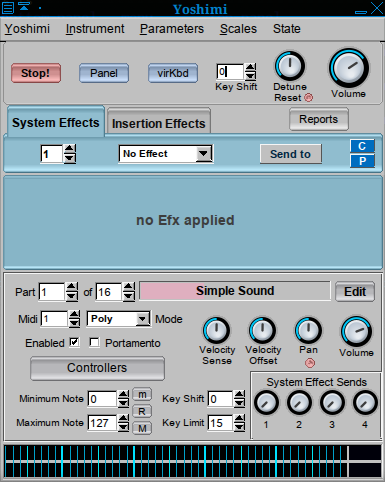
\includegraphics[scale=1.0]{1.3.5/yoshimi-first-screen.png}
   \caption{Yoshimi Main Screen, 1.3.5}
   \label{fig:yoshimi_main_screen}
\end{figure}

%  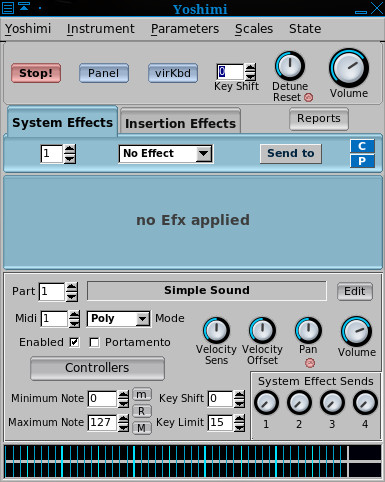
\includegraphics[scale=1.0]{yoshimi-first-screen.jpg}
%  This figure a bit out-of-date (it does not show the new "Part of"
%  feature)
   
   Then the \textsl{Yoshimi} main window appears, as shown in
   \figureref{fig:yoshimi_main_screen}.

   For this manual, we describe the main window as being composed of
   the following sections:

\begin{enumber}
   \item \textbf{Menu}.
   \item \textbf{Top Panel}.
   \item \textbf{Effects Panel}.
   \item \textbf{Bottom Panel}.  Includes the VU-meter at the bottom.
\end{enumber}

There's a lot going on with \textsl{Yoshimi}, and there's no way
to describe it in linear order.  This manual will describe how to do useful
things in each of the sections noted above, while leaving some of the
details to be described in later sections, to which reference can be made
for these details.  This document will depend heavily on index entries and
references.

% Important Concepts

%-------------------------------------------------------------------------------
% yum_concepts
%-------------------------------------------------------------------------------
%
% \file        yum_concepts.tex
% \library     Documents
% \author      Chris Ahlstrom
% \date        2015-06-15
% \update      2015-10-25
% \version     $Revision$
% \license     $XPC_GPL_LICENSE$
%
%     Provides the concepts.
%
%-------------------------------------------------------------------------------

\section{Concepts}
\label{sec:concepts}

   Before we start with the user-interface, let's cover some concepts.
   \textsl{Yoshimi} requires the user to understand many concepts.
   Understanding these concepts makes it easier to configure \textsl{Yoshimi}
   and to drive it from a sequencer application.
   
   Significant portions of this section are shamelessly copied (and tweaked)
   from Paul Nasca's original \textsl{ZynAddSubFX}
   manual \cite{zynodt} or \cite{zynpdf}.
   One can discern such sections by the usage of the term
   \textsl{ZynAddSubFX} instead of \textsl{Yoshimi}.
   However, even the \textsl{Yoshimi} developers sometimes
   refer to \textsl{ZynAddSubFX} or \textsl{Zyn}.

   Note that there are some audio/electrical concepts discussed in greater
   detail in
   \sectionref{sec:stock_settings_elements}.
   Perhaps they belong in this "concepts" section, but
   they are directly tied to user-interface items.

\subsection{Concepts / Terms}
\label{subsec:concepts_terms}

   This section doesn't provide comprehensive coverage of terms.  It
   covers mainly terms that puzzled the author at first.

\subsubsection{Concepts / Terms / cent}
\label{subsubsec:concepts_terms_cent}

   The \textbf{cent}
   \index{cent}
   is a logarithmic unit of measure used for musical
   intervals.  Twelve-tone equal temperament divides the octave into 12
   semitones of 100 cents each. Typically, cents are used to measure
   extremely small finite intervals, or to compare the sizes of comparable
   intervals in different tuning systems.
   The interval of one cent is much too small to be heard between
   successive notes.

\subsubsection{Concepts / Terms / frame}
\label{subsubsec:concepts_terms_frame}

   The \textbf{frame}
   \index{frame}
   is a single sample of however many channels an application is handling.
   If one is using JACK, a mono signal will have frames of 1 float, 2 floats
   for stereo, etc.

\subsubsection{Concepts / Terms / instrument}
\label{subsubsec:concepts_terms_instrument}

   \index{instrument}
   In \textsl{Yoshimi}, an \textsl{instrument} is a complex sound that can
   be constructed using ADDsynth, SUBsynth, PADsynth, and kits.
   Each instrument is loaded into a \textsl{part}
   (see section~\ref{subsubsec:concepts_terms_part}).

   In our documentation, we will sometimes use the terms "instrument",
   "patch", and even "program" interchangeably and loosely.
   However, "part" now has a different meaning, as seen in the next term.

\subsubsection{Concepts / Terms / part}
\label{subsubsec:concepts_terms_part}

   \index{part}
   In \textsl{Yoshimi}, a \textsl{part} is one of 64 slots into which one
   can load an instrument (see
   section~\ref{subsubsec:concepts_terms_instrument}).  Each part can be
   enabled or disabled, and assigned to a particular MIDI channel, one of 16
   channels.

   Note that the previous \textsl{Yoshimi} limit on parts was 16.
   Since around version 1.3.5, this limit has been raised.

\subsubsection{Concepts / Terms / patch}
\label{subsubsec:concepts_terms_patch}

   \index{patch}
   In MIDI jargon, a \textsl{patch} is a
   one of 16 channels in a MIDI device. Many synthesizers
   can handle several waveforms per patch, mixing different
   instruments together to create synthetic sounds. Each waveform counts as
   a MIDI voice. Some sound cards can support two or more waveforms per
   patch.  \textsl{Yoshimi} has some ability to combine waveforms ("voices")
   into one instrument (section~\ref{subsubsec:concepts_terms_instrument}),
   which can then be loaded into a
   \textsl{Yoshimi} part (section~\ref{subsubsec:concepts_terms_part}).

   Before General MIDI, which standardized patches, MIDI vendors assigned
   patch numbers to their synthesizer products in an arbitrary manner.

\subsubsection{Concepts / Terms / preset}
\label{subsubsec:concepts_terms_preset}

   \index{preset}
   In MIDI jargon, a \textsl{preset} is an instrument that can be easily
   loaded.
   It is also called a \textsl{program}
   (\ref{subsubsec:concepts_terms_program}).
   A program is selection via a "program-change" message.

   In \textsl{Yoshimi}, a \textsl{preset} is any collection of settings that
   can be saved to the clipboard or to a file, for later loading elsewhere.

\subsubsection{Concepts / Terms / program}
\label{subsubsec:concepts_terms_program}

   \index{program}
   In MIDI jargon, a \textsl{program} is the same as a \textsl{preset}
   (\ref{subsubsec:concepts_terms_preset}).

\subsubsection{Concepts / Terms / voice}
\label{subsubsec:concepts_terms_voice}

   \index{voice}
   In MIDI jargon, a \textsl{voice} is the same as
   a \textsl{preset} or a a \textsl{program}.

   In \textsl{Yoshimi}, a \textsl{voice} is a single configurable waveform
   that is just one of up to eight waveforms in an ADDsynth setting.
   Such voices can also be used as modulators for other voices.

\subsection{Concepts / ALSA Versus JACK}
\label{subsec:concepts_alsa_versus_jack}

   Some discusson from the \textsl{Yoshimi} wiki.  Here for eventual
   clarification.

   A bit of a question mark was raised over ALSA MIDI support. A lot of
   people seem to be giving this up and relying on bridges like
   \textsl{a2jmidi} for legacy software and hardware inputs. JACK MIDI is
   already synchronous so should be jitter-free whereas ALSA MIDI runs on a
   'best effort' basis. Added to which JACK is available for OS X and
   Windows so concentrating on this could make a possible port to other
   platforms more attractive -- not to me I (Will J. Godfrey) hasten to add!

   \textsl{Seq24} (a nice, if old, sequencer) uses ALSA MIDI. To connect
   applications that exclusively support JACK MIDI, \textsl{a2jmidid} will
   do the translation.  (Jack v. 1 has this integrated in recent versions,
   apparently).

   A frame is a single sample of however many channels one is handling, so if
   one is using JACK, a mono signal will have frames of 1 float, 2 for stereo,
   etc.

   ALSA is more complex as it handles the sound card's format, commonly integers
   (16 bit), 24 bit integers (low byte ignored), and short integers. Less
   commonly it may be floats or the weird 24 L ints. We're still not sure if
   these are packed or low-aligned (top byte ignored). We've assumed they are
   low aligned, but we don't know anyone who has such a card, in order to prove
   it.  As a matter of interest the only ALSA format \textsl{Yoshimi} doesn't
   support is float.

   Something that's not obvious is the way that ALSA audio is controlled and who
   takes command.  If one sets a specific destination, then \textsl{Yoshimi}
   says what it wants. It's often a negotiation on bit depth and channel count,
   but \textsl{Yoshimi} nearly always gets to decide the buffer size (it will be
   set to the internal buffer size).  However, if the destination is 'default'
   then ALSA decides on the sound card, bit depth, number of channels and the
   buffer size, and \textsl{Yoshimi} will set it's internal buffer size to
   match.  On most machines this always seems to be 1024.

\subsection{Concepts / Banks and Roots}
\label{subsec:concepts_banks_and_roots}

   In \textsl{Yoshimi}, a \textsl{root} is a location in which banks can be
   stored.  It is basically a directory, though it ultimately is assigned a
   number by \textsl{Yoshimi}, presumably to be able to access it in an
   automated way.  By choosing a root, one can hone in on a smaller
   collection of banks.
   
   Another important concept in \textsl{Yoshimi} is \textsl{banks}.
   Instruments can be stored in banks. These are loaded and saved
   automatically by the program.  On program start, the last used bank is
   loaded.
   \index{extended program}
   A single bank can store up to 128 instruments normally, and 160
   using extended programs.

   These concepts are discussed in great detail
   in \sectionref{sec:banks_and_roots}.

\subsection{Concepts / Sessions}
\label{subsec:concepts_sessions}

   As with most applications, \textsl{Yoshimi} and \textsl{ZynAddSubFX}
   allow for one to save one's work and reload it.
   Here are the file extensions used for saving the data:

   \begin{itemize}
      \item \texttt{.xmz}
         A Session. Everything.  It's format is either XML
         or compressed XML, as explained below.
         The \textbf{Parameters / Save} menu entry saves files with this
         extension.
         See \sectionref{paragraph:menu_yoshimi_settings_main_settings}.
      \item \texttt{.config}
         Sometimes one will see the extension \texttt{.config} used in the
         \texttt{\$HOME/.config/yoshimi} directory.
         These files contain information to translate between bank directory
         names and bank ID values.
      \item \texttt{.state}
         Sometimes one will see the extension \texttt{.state} used in the
         \texttt{\$HOME/.config/yoshimi} directory.
         These files contain a lot more information, that needed to
         duplicate a \textsl{Yoshimi} session that was saved.  Seems to be a
         superset of an \texttt{.xmz} file, saving everything.
      \item \texttt{.xiz}
         An Instrument.  These files can have two formats, compressed and
         uncompressed.
      \item \texttt{.xsz}
         Scale Settings.
         These files stored microtonal settings that \textsl{Yoshimi}
         can use to produce non-standard musical scales.
      \item \texttt{.xpz}
         Presets.
         A preset is canned version of a \textsl{Yoshimi} sub-setting.
         Presets can be copied and pasted using the
         \textbf{C} and \textbf{P} user-interface dialogs associated with many
         of the \textsl{Yoshimi} dialog windows.
         They make it easy to save portions of the current settings for later
         use.  For example, resonance settings can be saved.
   \end{itemize}

   The Unix \texttt{file} command indicates that these files are one of
   two types:

   \begin{itemize}
      \item \textsl{exported SGML document, ASCII text}.
         These files are unindented XML data with an encoding of UTF-8 and
         a DOCTYPE of "ZynAddSubFX-data".
      \item \textsl{gzip compressed data, from Unix}.
         These files can be renamed to end in ".gz", and then run through
         the \texttt{gunzip} program to yield the XML file (but without an
         \texttt{.xml} extension).
   \end{itemize}

   The format probably depends on the "XML compression level" option
   discussed in
   \sectionref{paragraph:menu_yoshimi_settings_main_settings}.

   \index{saving settings}
   Saving settings or not:
   If one changes settings and closes without saving, that means the settings
   remain in place only for the current session. If one has changed anything,
   when one closes \textsl{Yoshimi}, one will be given a second chance to
   save them. If one responds 'No',  the next time \textsl{Yoshimi} starts,
   the old settings will be restored.  An 'undo' feature would get pretty
   crazy very quickly.

   At some point in the future we may add a discussion of the contents of
   these files.  In general, the contents are structured a lot like the
   user-interface elements that are used to set them.

\subsubsection{Concepts / Sessions / All}
\label{subsec:concepts_sessions_all}

   One of the simplest ways to save one's work is to save the entire session.
   This can be done through the \textbf{Yoshimi} menu
   (the \textbf{File} menu in \textsl{ZynAddSubFX})
   and will result in the creation of
   an \texttt{.xmz} file. Once created, this file will hold the settings for
   all settings within that session, such as microtonal tunings, all
   patches, system effects, insertion effects, etc.

\subsubsection{Concepts / Sessions / Parts}
\label{subsec:concepts_sessions_parts}

   In \textsl{Yoshimi}, a \textsl{part} is one of 16 slots into which one
   can load an instrument (a patch or program).

   In many cases saving everything is not what is desired. Saving a patch
   later on in an editing session is one such example.
   In order to save a patch, one can either save it from the
   \textbf{Instruments} menu
   in \sectionref{subsubsec:menu_instrument_save},
   or through the \textbf{Bank} window in
   \sectionref{subsubsec:menu_instrument_show_banks}.

   With the \textbf{Instrument} menu, one can just save the file to any
   given location with the \texttt{.xiz} extension.

   With the \textbf{Banks} menu, one can assign a patch to a given slot with
   a bank.  This instrument will remain in that slot for future use until it is
   deleted. To see the physical location of the \texttt{.xiz} file, one
   should check the
   "Yoshimi / Settings / Banks / Root Dirs"
   (\textsl{File→Settings→Bank\_Root\_Dirs}) window to see the paths for
   banks.

   Note that one needs to have write permissions to add instruments to the
   bank.  Banks are more thoroughly described in
   \sectionref{subsec:concepts_banks_and_roots}.

\subsubsection{Concepts / Sessions / Presets}
\label{subsec:concepts_sessions_presets}

   Have a favorite setting for an envelope, or a difficult-to-reproduce
   oscillator? Then presets are for you! Presets allow for one to save the
   settings for any of the components which support copy/paste operations.
   This is done with preset files (\texttt{.xpz}), which get stored in the
   folders indicated by \textsl{File→Settings→Preset\_Root\_Dirs}.

\subsection{Concepts / Basic Synthesis}
\label{subsec:concepts_basics}

   This section describes some of the basic principles of synthesis,
   and contains suggestions on
   how to make instruments that sound like they have been made with
   professional equipment. This applies to \textsl{Yoshimi} or to any
   synthesizer (even if one wrote it oneself with a few lines of code). All
   the ideas from \textsl{Yoshimi} are derived from from the principles
   outlined below.

\begin{figure}[H]
   \centering 
   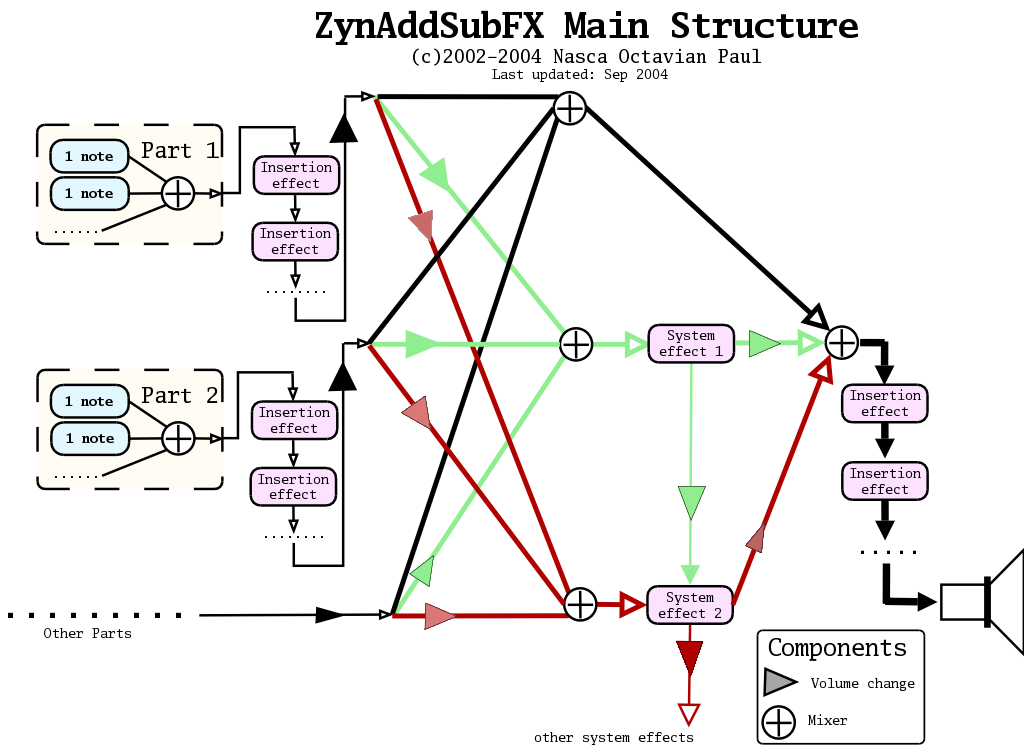
\includegraphics[scale=0.65]{zyn/zyn-diagram1.png}
   \caption{ZynAddSubFX/Yoshimi Main Structure}
   \label{fig:zynaddsubfx_main_structure}
\end{figure}

   For a given part, the synthesizer first creates a note.  Each note's
   waveform (for example, in a chord) is summed (mixed).  This complex
   waveform is then send to the series of Insertion effects (if any) that
   are defined.  Each part is then sent to a System effect and (depending on
   the wetness of the mix) directly to a mixer.  Additional Insertion
   effects (if any) are then applied.  The result is the final output of the
   synthesizer.

   The synthesizer has three major types of parameters: 

   \begin{enumber}
      \item \textbf{Master settings/parameters}.
         Contains all parameters (including effects and instruments).
      \item \textbf{Instrument parameters}.
         Contains ADDnote/SUBnote/PADnote parameters for a part.
      \item \textbf{Scale settings}.
         Contains the settings of scales (\textsl{Yoshimi}
         is a micro-tonal synth) and few other parameters related to
         tunings.
   \end{enumber}

\subsubsection{Concepts / Basic Synthesis / Panning}
\label{subsubsec:concepts_basics_panning}

   Pan lets one apply panning, which means that the sound source can move to
   the right or left. Set it to 0.0 to only hear output on the right side, or
   to the maximum value to only hear output on the left side.

\subsubsection{Concepts / Basic Synthesis / Wetness}
\label{subsubsec:concepts_basics_wetness}

   Wetness determines the mix of the results of the effect and its input.
   This mix is made the effects output. If an effect is wet, it means that
   none of the input signal is bypassing the effect. If it is dry, then
   the effect is bypassed completely, and has no effect.

\subsubsection{Concepts / Basic Synthesis / Single Note}
\label{subsubsec:concepts_basics_single_note}

   The idea of this synthesis model is from another synthesizer Paul Nasca
   wrote years ago, released on the Internet as "Paul's Sound
   Designer".  The new model is more advanced than that project
   (adding SUBsynth, more LFO's/Envelopes, etc.), but the idea is
   the same.

\begin{figure}[H]
   \centering 
   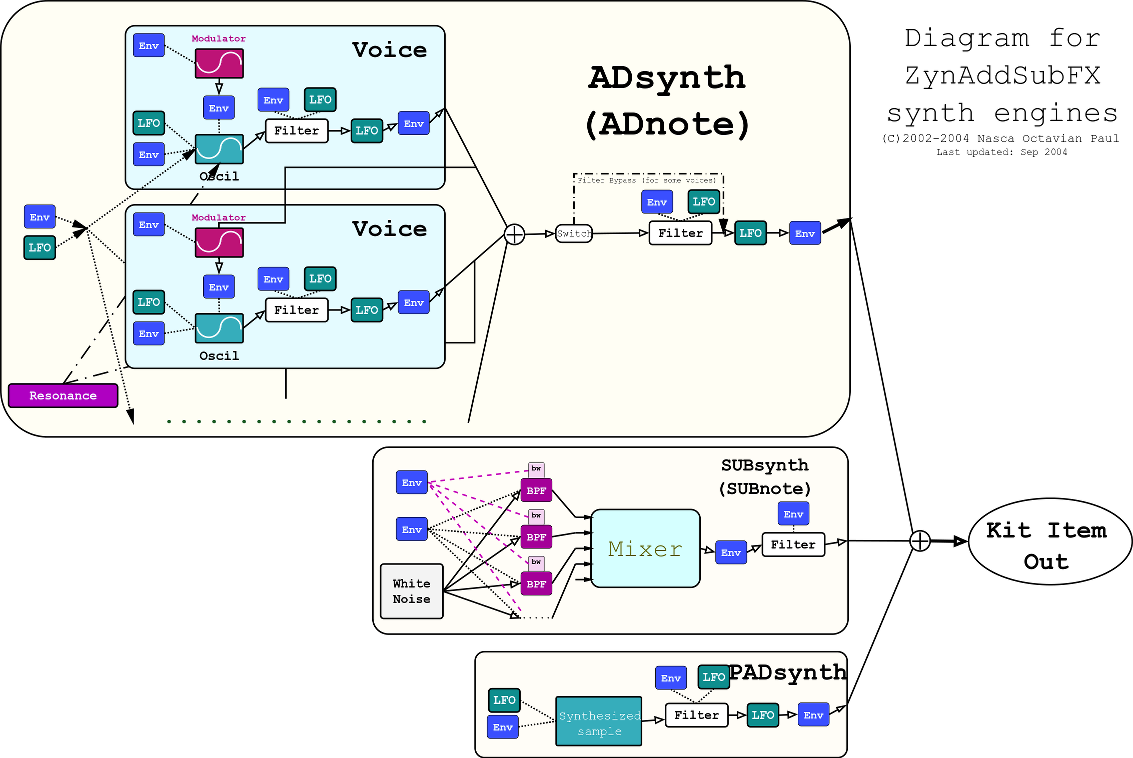
\includegraphics[scale=0.4]{zyn/zyn-adnote-diagram2.png}
   \caption{ZynAddSubFX/Yoshimi Note Generation}
   \label{fig:zynaddsubfx_note_generation}
\end{figure}
   
   The figure represents the synthesizer module components. The continuous
   lines are the signal routing, and the dotted lines are frequency
   controlling signals (they controls the frequency of something).  The
   dashed lines controls the bandwidths of bandpass filters. "Env" are the
   envelopes, "LFO" the Low Frequency Oscillators, "BPF" are band pass
   filters, "bw" are the bandwidth of the BPF's.  If one uses instrument kits,
   the "note out" represents the output of the kit item.

\subsubsection{Concepts / Basic Synthesis / Harmonics}
\label{subsubsec:concepts_basics_harmonics}

   Harmonics are sine waves that are multiple of the base frequency of a
   note.  \textsl{Yoshimi} and \textsl{ZynAddSUbFX} introduce the concept of
   increasing the bandwidth of a harmonic so that it is not quite a sine
   wave.

\paragraph{Harmonic Bandwidth}
\label{paragraph:concepts_basics_harmonic_bandwidth}

   "Harmonic bandwidth" does not refer to sample-rate, it refers to the
   frequency "spread" of each harmonic. This is the most important principle
   of making instruments that sound good. Unfortunately there is very little
   documentation about it.
    
   Often it is believed that the pitched sounds (like piano, organ, choir,
   etc.) for a single note have a frequency, but it's actually
   harmonics and nothing more. Many people try to synthesize a sound using an
   exact frequency plus the harmonics, and observe that the result sounds too
   "artificial".  They might try to modify the harmonic content, add a
   vibrato, tremolo, but even that doesn't sound "warm" enough. The reason is
   that the natural sounds don't produce an exact periodic; their sounds are
   quasi-periodic.  Please notice that not all quasi-periodic sounds are
   "warm" or pleasant.
   (Nasca's discussion of periodic vs. quasi-periodic,
   and the figures he shows, are not included here.)
   Basically, by slightly increasing the bandwidth of a periodic sound, it
   is possible to make it quasi-periodic.

   A very important thing about bandwidth and natural sounds is that the
   bandwidth has to be increased if one increases the frequency of the
   harmonic.  If the fundamental frequency is 440 Hz and the bandwidth is 10
   Hz (that means that the frequencies are spread from 435 to 445 Hz), the
   bandwidth of the second harmonics (880Hz) must be 20 Hz. A simple formula
   to compute the bandwidth of each harmonic if one knows the bandwidth of the
   fundamental frequency is \(BWn = n⋅bw1\), where \texttt{n} is the
   order of the harmonic, \texttt{bw1} is the bandwidth of fundamental
   frequency and \texttt{BWn} is the bandwidth of the n'th harmonic. If one
   does not increase the bandwidth according the frequency, the resulting
   instrument will (usually) sound too 'artificial' or 'ugly'.  There
   are at least three methods of making good sounds with the above
   considerations: 

   \begin{enumber}
      \item \textbf{Detuning}.
      By adding slightly detuned sounds (in \textsl{Yoshimi}
      it is called "ADDsynth"). The idea is not new: it has been used
      for thousands of years in choirs and ensembles. That's why choirs
      sound so beautiful.
      \item \textbf{Noise sculpting}.
      By generating white noise, subtracting all harmonics with band-pass
      filters and adding the results (in \textsl{Yoshimi}
      it is called "SUBsynth").
      \item \textbf{Generation by spectrum}.
      By "drawing" the above graph that represents the frequency
      amplitudes on a large array, put random phases and do a single
      IFFT for the whole sample.
   \end{enumber}

\paragraph{Harmonic Amplitude}
\label{paragraph:concepts_basics_harmonic_amplitude}

   An important principle of natural harmonics is to decrease the amplitude
   of higher harmonics on low-velocity notes.

   All natural notes have this property, because on low-velocity notes there
   is not enough energy to spread to higher harmonics. On artificial
   synthesis one can do this by using a low-pass filter that lowers the
   cutoff frequency on notes with low velocities or, if one uses FM
   (frequency modulation), by lowering the modulator index. 
   The spectrum of the sound should be almost the same according to
   the frequencies and not the harmonics.

   This means that, for example, the higher the pitch is, the smaller the
   number of harmonics it will contain. This happens in a natural instrument
   because of the resonance. 
   In this case there are many instruments that don't obey this, but sound
   quite good (example: synth organ). 
   If one records the C-2 note from a piano and one plays it at a very high
   speed (8 times), the result will not sound like the C-5 key from the
   piano. The pitch is C-5, but the timbre is very different. This is because
   the harmonic content is preserved (the n-th harmonic will have the
   same amplitude in both cases) and not the spectrum (eg. the
   amplitudes of the harmonics around 1000 Hz are too different from
   one case to another). 

   In artificial synthesis one can use filters to add resonance or FM
   synthesis that varies the index according to the frequency.  In
   \textsl{Yoshimi} one can add the resonance:

   \begin{enumber}
      \item \textbf{ADDsynth}:
      Use the Resonance, a high harmonics sound content, and filters or FM.
      \item \textbf{SUBsynth}:
      Add some harmonics and use the Global Filter.
   \end{enumber}

\subsubsection{Concepts / Basic Synthesis / Randomness}
\label{subsubsec:concepts_basics_randomness}

   The main reason why the digital synthesis sounds too "cold" is because the
   same recorded sample is played over and over on each key-press.  There is
   no difference between a note played the first time and second time.
   Exceptions may be the filtering and some effects, but these are not
   enough. In natural or analogue instruments this doesn't happen because
   it is impossible to reproduce exactly the same conditions for each
   note. To make a warm instrument one must make sure that it sounds
   slightly different each time. In \textsl{Yoshimi}
   one can do this:

   \begin{enumber}
      \item \textbf{ADDsynth}:
      Set the "Randomness" function from Oscillator Editor
      to a value different than 0, or change the start phase of the LFO to
      the leftmost value.
      \item \textbf{SUBsynth}:
      All notes already have randomness because the
      starting sound is white noise.
      \item \textbf{PADSynth}:
      The engine starts the sample from random positions
      on each keystroke.
   \end{enumber}

   In setting the randomness of the oscillator output, there are two types of
   randomness. The first is \textsl{group randomness}, where the oscillator
   starts at a random position. The second is \textsl{phase randomness}:
   from -64 (max) to -1 (min) and each harmonic (the oscillator is phase
   distorted) is from 1 (min) to 63 (max). 0 is no randomness. One
   could use this parameter for making warm sounds like analogue
   synthesizers.

   See the ADDSynth oscillator editor for this kind of
   control, named \textbf{Ph.rnd} or \textbf{rnd}.

   There is now the possibility to add a 'naturalising' random pitch element
   to a part. This is found in the part-edit window. The settings are not
   currently saved, but will be once the control values are settled, and
   there has been enough experience to decide whether it should be a part or
   voice setting.

\subsubsection{Concepts / Basic Synthesis / Components}
\label{subsubsec:concepts_basics_components}

   \textsl{Important}:
   All indexes of MIDI Channels, Parts, Effects starts from 0, so, for
   example, the first Part is 0.

   \textsl{Yoshimi} components:

   \begin{enumber}
      \item \textbf{Parts}.
         They receive the note messages from MIDI
         Channels. One may assign a part to any channel. A part can store
         only one instrument.  "Add.S" represents ADDsynth and "Sub.S" is
         SUBsynth.  In recent versions of \textsl{Yoshimi}, the number of
         parts available has been increased from 16 to 64.
      \item \textbf{Insertion Effect}.
         This effect applies only to one part; one can have any number of
         insertion effects for one part, but the number of these cannot be
         bigger than NUM.INS.EFX.
      \item \textbf{Part Mixer}.
         Mixes all parts.
      \item \textbf{System Effects}.
         Applied to all parts, one can set how much signal
         is routed through a system effect.
      \item \textbf{Master mixer}.
         Mixes all outputs of Parts Mixers and System Effects.
   \end{enumber}

\subsubsection{Concepts / Basic Synthesis / Filters}
\label{subsubsec:concepts_basics_filters}

   \textsl{Yoshimi}
   offers several different types of filters, which can be used
   to shape the spectrum of a signal. The primary parameters that affect the
   characteristics of the filter are the cutoff, resonance, filter stages,
   and the filter type.

   \textbf{Cutoff}:
   This value determines which frequency marks the changing point for
   the filter. In a low pass filter, this value marks the point where higher
   frequencies are attenuated.

   \textbf{Resonance}:
   The resonance of a filter determines how much excess energy is
   present at the cutoff frequency. In \textsl{Yoshimi},
   this is represented by the Q-factor, which is defined to be the cutoff
   frequency divided by the bandwidth. In other words higher Q values result
   in a much more narrow resonant spike.

   \textbf{Stages}:
   The number of stages in a given filter describes how sharply it is
   able to make changes in the frequency response.
   The affect of the order of the filter is roughly synonymous with the
   number of stages of the filter. For more complex patches it is important
   to realize that the extra sharpness in the filter does not come for free
   as it requires many more calculations being performed. This phenomena is
   the most visible in SUBsynth, where it is easy to need several hundred
   filter stages to produce a given note.

   The \textbf{Q}:
   value of a filter affects how concentrated the signal’s energy is at
   the cutoff frequency.
   For many classical analog sounds, high Q values were used on sweeping
   filters. A simple high Q low pass filter modulated by a strong envelope is
   usually sufficient to get a good sound.

   \textbf{Filter Type}:
   There are different types of filters. The number of poles define what will
   happen at a given frequency. Mathematically, the filters are functions
   which have poles that correspond to that frequency. Usually, two poles
   mean that the function has more "steepness", and that one can set the
   exact value of the function at the poles by defining the "resonance
   value". Filters with two poles are also often referenced as Butterworth
   filters.

   For the interested reader, functions having \textsl{poles}
   means that we are given a quotient of polynomials. The denominator has
   degree 1 or 2, depending on the filter having one or two poles. In the
   file \texttt{DSP/AnalogFilter.cpp},
   \texttt{AnalogFilter::computefiltercoefs()} sets the coefficients
   (depending on the filter type), and
   \texttt{AnalogFilter::singlefilterout()} shows the whole polynomial (in a
   formula where no quotient is needed).

   Filters are thoroughly described in
   \sectionref{subsec:filter_settings}.

\subsubsection{Concepts / Basic Synthesis / Envelopes}
\label{subsubsec:concepts_basics_envelopes}

   Envelopes are long-period wave forms that are applied to frequency,
   amplitude, or filters.  Envelopes generate effects such as tremolo and
   vibrato, as well as effects that occur when a sound-generating physical
   component changes shape.
   Envelopes are thoroughly described in
   \sectionref{subsec:envelope_settings}.

\subsection{Concepts / MIDI}
\label{subsec:concepts_midi}

   It is useful to discuss some of the details of MIDI in order
   to understand \textsl{Yoshimi}.  Obviously, we assume
   some knowledge already, or one wouldn't be running
   \textsl{Yoshimi}.

\subsubsection{Concepts / MIDI / Messages}
\label{subsubsec:concepts_midi_messages}

   \textsl{Yoshimi} responds to the following MIDI messages.

   \begin{table}
      \centering
      \caption{ZynAddSubFX/Yoshimi MIDI Messages}
      \label{table:zynaddsubfx_midi_messages}
      \begin{tabular}{r l}
         \textbf{0} or \textbf{32} &
            Bank Change (user selectable, does \textsl{not} force a program
            change) \\
         \textbf{1} & Modulation Wheel \\
         \textbf{7} & Volume \\
         \textbf{10} & Panning \\
         \textbf{11} & Expression \\
         \textbf{64} & Sustain pedal \\
         \textbf{65} & Portamento On/Off \\
         \textbf{71} & Filter Q (Sound Timbre) \\
         \textbf{74} & Filter Cutoff (Brightness) \\
         \textbf{75} & BandWidth (different from GM spec) \\
         \textbf{76} & FM amplitude (different from GM spec) \\
         \textbf{77} & Resonance Center Frequency (different from GM spec) \\
         \textbf{78} & Resonance Bandwith (different from GM spec) \\
         \textbf{120} & All Sounds OFF \\
         \textbf{121} & Reset All Controllers \\
         \textbf{123} & All Notes OFF \\
         \textbf{192} & Program Change (voices 1-128) \\
         \textbf{224} & Pitch Bend \\
      \end{tabular}
   \end{table}

   For the controllers that are not defined in GM:

   \begin{itemize}
      \item \textbf{Bandwidth} control (75) increases or decreases the bandwidth
      of instruments. The default value of this parameter is 64. 
      \item \textbf{Modulation amplitude} (76) decreases the amplitude of
      modulators on ADDsynth. The default value of this parameter is 127. 
      \item \textbf{Resonance Center Frequency} control (77) changes the center
      frequency of the resonance. 
      \item \textbf{Resonance Bandwidth} control (78) changes the bandwidth of the
      resonance. 
   \end{itemize}

   The Program Change (192) also provides user selectable CC for voices
   128-160.  There is now an option to make Program Change enable a part if
   it's currently disabled.

   User selectable CC for Bank Root Path change.
   For more details of bank changes see
   \sectionref{subsec:concepts_banks_and_roots}.

   Instruments inside banks should \textsl{always} have file-names that
   begin with four digits,  followed
   by a hyphen. Otherwise the results can be rather unpredictable.

\subsubsection{Concepts / MIDI / NRPN}
\label{subsubsec:concepts_midi_nrpn}

   NRPN stands for "Non Registered Parameters Number".
   NRPNs can control all System and Insertion effect parameters.
   Using NRPNs, \textsl{Yoshimi} can now directly set some part values
   regardless of what channel that part is connected to.  For example, one
   may change the reverb time when playing to keyboard, or
   change the flanger's LFO frequency.

   NRPNs are described in greater detail in section
   \sectionref{sec:nrpns}.

\paragraph{Concepts / MIDI / NRPN / Vector Control}
\label{paragraph:concepts_midi_nrpn_vector_control}

   Vector control is a way to control more than one part with the
   controllers.
   Vector control is only possible if one has 32 or 64 parts active 
   in \textsl{Yoshimi}.
   In vector mode, parts will still play together but the vector controls can
   change their volume, pan, filter cutoff in pairs, controlled by user
   defined CCs set up with NRPNs.

   Vector control is described in greater detail in section
   \sectionref{subsection:vector_control}.

\paragraph{Concepts / MIDI / NRPN / Effects Control}
\label{paragraph:concepts_midi_nrpn_effects_control}

   NRPNs are very useful in modifying the parameters of the
   \textsl{Yoshimi} effects.

   Effects control is described in greater detail in section
   \sectionref{subsection:nrpns_midi_nrpn_effects_control}.

\subsection{Concepts / LV2 Plugin}
\label{subsec:concepts_lv2_plugin}

   \textsl{Yoshimi} now runs as an LV2 plugin.

   TODO: Describe LV2 at a high-level.

%-------------------------------------------------------------------------------
% vim: ts=3 sw=3 et ft=tex
%-------------------------------------------------------------------------------


% Menu

%-------------------------------------------------------------------------------
% yum_menu
%-------------------------------------------------------------------------------
%
% \file        yum_menu.tex
% \library     Documents
% \author      Chris Ahlstrom
% \date        2015-05-11
% \update      2016-06-05
% \version     $Revision$
% \license     $XPC_GPL_LICENSE$
%
%     Provides the Menu section of yoshimi-user-manual.tex.
%
%-------------------------------------------------------------------------------

\section{Menu}
\label{sec:menu}

   At last, we're now ready to describe the user-interface of \textsl{Yoshimi}!
   The \textsl{Yoshimi} menu, as seen at the top of
   \figureref{fig:yoshimi_main_screen},
   is fairly simple, but it is important to understand the
   structure of the menu entries.

\subsection{Menu / Yoshimi}
\label{subsec:menu_yoshimi}

   The \textsl{Yoshimi}
   menu entry contains the sub-items shown in
   \figureref{fig:yoshimi_menu_items}.
   The next few sub-sections discuss the sub-items in the 
   \textsl{Yoshimi} sub-menu.
   (Note that, in \textsl{ZynAddSubFX}, this menu is called the
   \textsl{File} menu.)

\begin{figure}[H]
   \centering 
%  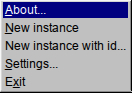
\includegraphics[scale=0.75]{menu/yoshimi-menu-yoshimi.jpg}
   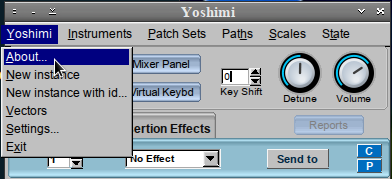
\includegraphics[scale=1.0]{1.4.0/yoshimi-menu-yoshimi.png}
   \caption{Yoshimi Menu Items}
   \label{fig:yoshimi_menu_items}
\end{figure}

   \textbf{New:}
   \index{new!Vector menu entry}
   New with version 1.4.0 of \textsl{Yoshimi} is the \textbf{Vectors} menu
   entry.
   See \sectionref{subsubsec:menu_yoshimi_vectors}, which presents this dialog
   and briefly describes it.

   \textbf{Bug:}
   \index{bugs!menu hot keys don't work}
   There seems to be a bug in that the expected menu hot-keys
   (Alt-Y, Alt-I, Alt-P, and Alt-S) do not work (Yoshimi 1.3.5).

\subsubsection{Menu / Yoshimi / About...}
\label{subsubsec:menu_yoshimi_about}

   There is no \textbf{Help} menu in \textsl{Yoshimi}.  Therefore, the
   \textbf{About} dialog appears in the \textbf{Yoshimi} menu, as shown in
   \figureref{fig:yoshimi_about_dialog}.
   These guys need some acknowledgment for their hard work!
   And they acknowledge the massive groundwork laid by the
   \textsl{ZynAddSubFX} project.

\begin{figure}[H]
   \centering 
%  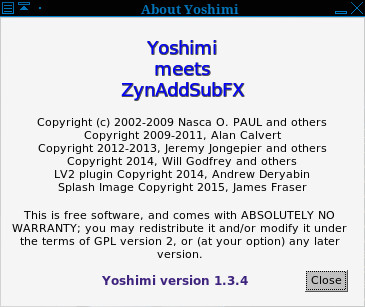
\includegraphics[scale=1.0]{menu/Yoshimi/yoshimi-about.jpg}
   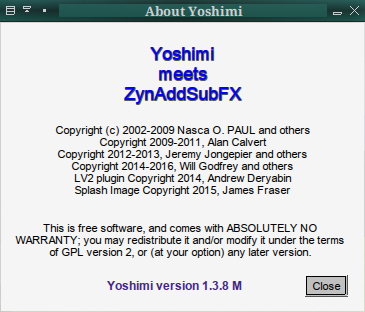
\includegraphics[scale=1.0]{1.3.8/yoshimi-about.jpg}
   \caption{Yoshimi Menu, About Dialog}
   \label{fig:yoshimi_about_dialog}
\end{figure}

\subsubsection{Menu / Yoshimi / New instance}
\label{subsubsec:menu_yoshimi_new_instance}

   Creates a new instance of \textsl{Yoshimi}.
   If JACK is running,
   start a normal (JACK-using) instance of \textsl{Yoshimi}.
   Then use this menu entry.  \textsl{Yoshimi} will start another instance
   of itself, with an ID of 1.
   This instance can be verified by running a JACK session manager such as
   QJackCtl.

   It is important to note that each instance of \textsl{Yoshimi} has its
   own configuration file.  Each also has its own MIDI and audio ports.
   Thus, these instances are partly independent of each other.

   Opening a new instance creates a copy that has it's own dynamic memory for
   running storage. In the future, some data (such as recent history) will be
   shared between instances. This will be done only where instances actually
   need to be in sync.

   Each instance has it's own file-store in \textsl{Yoshimi}'s configuration
   directory. The means that if one opens a numbered instance, one will get
   back all the settings that were previously used for that instance.

   Instances no longer fight for access to JACK/ALSA audio; they will simply
   try to find another route to a soundcard. Failing to find one,
   they will revert to null audio, but will nonetheless start cleanly.

\subsubsection{Menu / Yoshimi / New instance with id...}
\label{subsubsec:menu_yoshimi_new_instance_with_id}

   Creates a new instance of \textsl{Yoshimi}
   with an ID that is a number.
   See \figureref{fig:yoshimi_instance_dialog}.
   It tries to open a \textsl{Yoshimi} instance based on the configuration
   found in the file
   \texttt{\textasciitilde/.config/\-yoshimi/\-yoshimi.configXX}, where
   \textsl{XX} is the ID one supplied.

\begin{figure}[H]
   \centering 
   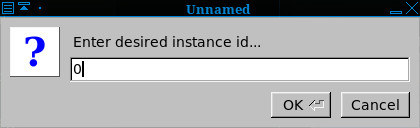
\includegraphics[scale=0.75]{menu/Yoshimi/yoshimi-instance-id.jpg}
   \caption{Yoshimi Menu, Instance Dialog}
   \label{fig:yoshimi_instance_dialog}
\end{figure}

   Useful when connecting devices with JACK.
   Start a normal (JACK-using) instance of \textsl{Yoshimi}.
   Then use this menu entry, supply a number as an ID.
   \textsl{Yoshimi} will start another instance
   of itself, with an ID of whatever number one specified.
   This instance can be verified by running a JACK session manager such as
   \textsl{QJackCtl}.

   In a non-JACK setup it won't fail, but in the absence of any specific
   setting, it will have null audio, but (probably) will still connect to ALSA
   MIDI.  Not too useful, but we should test that sometime.

\subsubsection{Menu / Yoshimi / Vectors}
\label{subsubsec:menu_yoshimi_vectors}

   Vectors provide a way of mixing up to four parts in a manner that can be
   automatec, saved, and loaded.  The features of vector control are presented
   in \sectionref{sec:vector}.
   Vector setup and control from the \textsl{Yoshimi} command-line are
   discussed in
   \sectionref{subsec:command_line_command_level}.
   Here, we discuss the vector configuration dialog.
   (As an exercise, one can compare the various functions of the vector dialog
   to the command-line commands one can use to set up the vector
   functionality.)
   The new \textbf{Yoshimi / Vectors} menu entry brings up the following
   dialog:

\begin{figure}[H]
   \centering 
   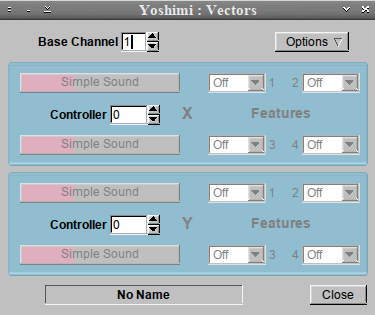
\includegraphics[scale=0.75]{1.4.0/yoshimi-vectors-dialog.png}
   \caption{Yoshimi Vectors Dialog}
   \label{fig:yoshimi_vectors_dialog}
\end{figure}

   The user-interface items in the vector dialog are:

   \begin{enumber}
      \item \textbf{Top Line}
      \begin{enumber}
         \item \textbf{Base Channel}
         \item \textbf{Options}
      \end{enumber}
      \item \textbf{X Vector}
      \begin{enumber}
         \item \textbf{Controller} (CC Event)
         \item \textbf{Part 1}
         \item \textbf{Part 2}
         \item \textbf{Features}
         \begin{enumber}
            \item \textbf{Feature 1} (Volume)
            \item \textbf{Feature 2} (Pan)
            \item \textbf{Feature 3} (Brightness)
            \item \textbf{Feature 4} (Modulation)
         \end{enumber}
      \end{enumber}
      \item \textbf{Y Vector}
      \begin{enumber}
         \item \textbf{Controller} (CC Event)
         \item \textbf{Part 1}
         \item \textbf{Part 2}
         \item \textbf{Features}
         \begin{enumber}
            \item \textbf{Feature 1} (Volume)
            \item \textbf{Feature 2} (Pan)
            \item \textbf{Feature 3} (Brightness)
            \item \textbf{Feature 4} (Modulation)
         \end{enumber}
      \end{enumber}
      \item \textbf{Bottom Line}
      \begin{enumber}
         \item \textbf{Vector Name}
         \item \textbf{Close}
      \end{enumber}
   \end{enumber}

   Although they are nested, for simplicity we will discuss the unique items
   serially.

   \setcounter{ItemCounter}{0}      % Reset the ItemCounter for this list.

   \itempar{Base Channel}{Vectors!base channel}
   Vector Base Channel.
   This item specifies the MIDI channel on which the vector (of parts) will be
   based.  This channel is the incoming MIDI channel to which the vector setup
   will respond to on all parts.

   Values: \texttt{1 to 16, 1*}

   \itempar{Options}{Vectors!options}
   Vector Options.

   Values: \texttt{1 to 127, 64*}

\begin{figure}[H]
   \centering 
   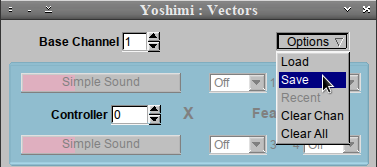
\includegraphics[scale=0.75]{1.4.0/yoshimi-vectors-options.png}
   \caption{Yoshimi Vectors Options}
   \label{fig:yoshimi_vectors_options}
\end{figure}

   The menu entries provide the actions described in this list:

   \begin{enumber}
      \item \textbf{Load}.
         Brings up a file dialog that let's one pick an arbitary vector file
         (extension \texttt{.xvy}) in an arbitrary directory, or select a
         "Favorites" directory in which to look for vector files.
         The base name of the file is then shown in the \textbf{Vector Name}
         field.
      \item \textbf{Save}.
         Brings up a file dialog that let's one save an arbitary vector file
         (extension \texttt{.xvy}) in an arbitrary directory, or select a
         "Favorites" directory in which to save a vector file.
         The base name of the file is then shown in the \textbf{Vector Name}
         field.
      \item \textbf{Recent}.
         Brings up a short list of the previous vector files dealt with.
      \item \textbf{Clear Chan}.
         Clears the base channel number????
      \item \textbf{Clear All}.
         Clears out the full vector setup, rendering it an "empty" vector setup
         that cannot be saved.
   \end{enumber}

   \itempar{X Vector}{Vectors!x}
   The X Vector.
   This vector provides the minimal setup for a vector.  This setup requires
   \textsl{Yoshimi} to be configured for 32 parts, to be able to fully support
   a two-part vector for every MIDI channel.  This section is disabled until
   selects a \textbf{Controller} event value for it.

   \itempar{Controller}{Vectors!controller}
   Vector Controller CC Event.
   If 0, the section (\textbf{X} or \textbf{Y}) that this value is in is
   disabled.  Otherwise, the number is the MIDI continuous controller (CC)
   event value that is to be used to control the mix of the two parts involved
   in this vector.

   Values: \texttt{1 to 119, 0*}

   \itempar{Part 1}{Vectors!part 1}
   Part 1.
   The top button in the section (\textbf{X} or \textbf{Y}) selects the first
   part to use in the two-part vector.  Clicking this button brings up the
   default bank dialog.  This dialog allows one to select a part (instrument),
   or to select an different bank from which to choose a part (instrument).

   \itempar{Part 2}{Vectors!part 2}
   Part 2.
   The bottom button in the section (\textbf{X} or \textbf{Y}) selects the
   second part to use in the two-part vector.  Clicking this button brings up
   the default bank dialog, just as for the \textbf{Part 1} button.

   \itempar{Feature 1}{Vectors!volume}
   Vector Feature 1, Volume.
   This feature can be disabled, or enabled.  Feature 1 is always fixed as MIDI
   event 7 (volume), and is not reversible.
   When enabled, the volume is traded off between the first part and second part
   as the selected MIDI CC controller event data value changes.
   While the first part increases in volume, the second part decrease in
   volume, and vice versa.

\begin{figure}[H]
   \centering 
   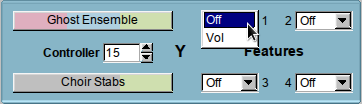
\includegraphics[scale=0.75]{1.4.0/yoshimi-vectors-feature-1.png}
   \caption{Yoshimi Vectors, Feature 1}
   \label{fig:yoshimi_vectors_feature_1}
\end{figure}

   Values: \texttt{Off*, Vol}

   Note that the common theme between all features is that they apply inversely
   to the two parts/instruments that are paired in an \textbf{X}
   or \textbf{Y} vector.

   \itempar{Feature 2}{Vectors!pan}
   Vector Feature 2, Pan.
   This feature can be disabled, enabled, or reversed.
   When enabled, it acts similarly to volume, panning from left to right as the
   data value increases.
   When reversed, it pans from right to left as the data value increases.

\begin{figure}[H]
   \centering 
   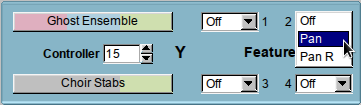
\includegraphics[scale=0.75]{1.4.0/yoshimi-vectors-feature-2.png}
   \caption{Yoshimi Vectors, Feature 2}
   \label{fig:yoshimi_vectors_feature_2}
\end{figure}

   Values: \texttt{Off*, Pan, Pan R}

   \itempar{Feature 3}{Vectors!brightness}
   Vector Feature 3, Brightness.
   Brightness here refers to the application of a (we presume) low-pass filter
   with a varying cutoff frequency.
   This feature can be disabled, enabled, or reversed.
   When enabled, it acts similarly to volume, changing the brightness
   from left to right as the data value increases.
   When reversed, it changes the brightness from right to left as the data
   value increases.

\begin{figure}[H]
   \centering 
   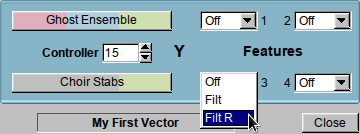
\includegraphics[scale=0.75]{1.4.0/yoshimi-vectors-feature-3.png}
   \caption{Yoshimi Vectors, Feature 3}
   \label{fig:yoshimi_vectors_feature_3}
\end{figure}

   Values: \texttt{Off*, Filt, Filt R}

   \itempar{Feature 4}{Vectors!modulation}
   Vector Feature 4, Modulation.
   Modulation here refers to the application of an (we presume) LFO
   (for amplitude or frequency) with a varying modulation depth.
   This feature can be disabled, enabled, or reversed.
   When enabled, it acts similarly to volume, changing the modulation
   from left to right as the data value increases.
   When reversed, it changes the modulation from right to left as the data
   value increases.

\begin{figure}[H]
   \centering 
   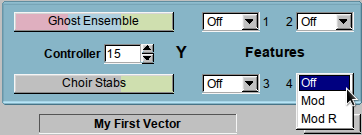
\includegraphics[scale=0.75]{1.4.0/yoshimi-vectors-feature-4.png}
   \caption{Yoshimi Vectors, Feature 4}
   \label{fig:yoshimi_vectors_feature_4}
\end{figure}

   Values: \texttt{Off*, Mod, Mod R}

   \itempar{X Vector}{Vectors!x}
   The X Vector.
   This vector provides the maximal setup for a vector.  This setup requires
   \textsl{Yoshimi} to be configured for 64 parts, to be able to fully support
   an additional two-part vector for every MIDI channel.  This section is
   disabled until selects a \textbf{Controller} event value for it.

   Other than that, the \textbf{Y} vector acts like the \textbf{X} vector, and
   all of the sub-items have the same functionality as in the
   \textbf{X} vector.

\begin{figure}[H]
   \centering 
   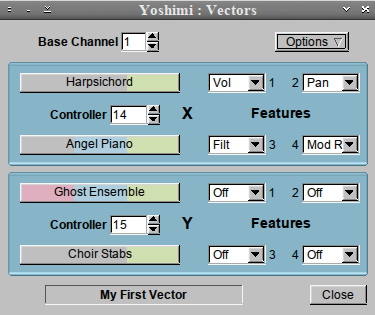
\includegraphics[scale=0.75]{1.4.0/yoshimi-vectors-saved.png}
   \caption{Yoshimi Vectors Saved as "My First Vector"}
   \label{fig:yoshimi_vectors_saved}
\end{figure}

   If starting a new vector setup, first
   select the base channel (1 to 16) to set the vector on. Next,
   use the \textbf{X} and \textbf{Y} \textbf{Controller}
   spin-boxes to select the incoming CC.
   If you set an invalid one strange things may happen, though it won't
   actually do any harm.

   The instrument buttons bring up the instrument list window in exactly the same
   way as the main part one does, but do not currently the right-click
   windows return feature.

   When setting up a completely new vector, if the mixer or the main part are
   visible, they may be slightly out of sync, but will correct themselves as
   soon as one changes an instrument or part.

   When one \textbf{clears} a vector it doesn't delete loaded voices, nor does
   it change the active status of the part, nor the number of parts available.
   This is because these settings may have been made independent of vector
   control. In short, vector setup will add things but not remove them.

\subsubsection{Menu / Yoshimi / Settings...}
\label{subsubsec:menu_yoshimi_settings}

   The \textsl{Yoshimi Settings} dialog contains four tabs that control the
   major and overall settings of \textsl{Yoshimi}.  At the bottom of this
   dialog are two buttons:
   \textbf{Save and Close} and \textbf{Close Unsaved}.
   \index{Save and Close}
   \index{Close Unsaved}

   Please note that the \textbf{Save and Close} and \textbf{Close Unsaved}
   buttons apply to the \textsl{whole}
   \textbf{Settings} window.
   Furthermore, the "saving" does \textsl{not} refer to preserving the changes
   that have been made
   in any of the tabs for the current \textsl{Yoshimi} session.  Any changes
   made in \textbf{Settings} always remain in place for the current
   \textsl{Yoshimi} session.
   However, the changes to the settings are saved to
   the state file \textsl{only} if \textbf{Save and Close} is clicked.

   \setcounter{ItemCounter}{0}      % Reset the ItemCounter for this list.

   \itempar{Save and Close}{Settings!Save and Close}
   This selection saves the settings made in \textbf{all} of the tabs to the
   state file, and closes the \textsl{Yoshimi} settings dialog.

   \itempar{Close Unsaved}{Settings!Close Unsaved}
   Close Unsaved, Main Settings.

   This selection closes the \textsl{Yoshimi} settings dialog.
   However, note that any changes made in the tabs
   \textsl{are preserved}.  They are preserved for the current
   \textsl{Yoshimi} session, but are not saved to the filesystem.
   
\paragraph{Menu / Yoshimi / Settings / Main Settings}
\label{paragraph:menu_yoshimi_settings_main_settings}

   The Main Settings tab controls the main configuration items that
   follow, which apply to all patches/instruments.
   The main settings are shown in
   \figureref{fig:yoshimi_main_settings_dialog}.

   Some settings only take effect after restarting the synthesizer.
   In Main settings, only items marked with an asterisk ('*')
   need a restart. 
   (This in now only the first two. Some of the other ones had
   prevously been wrongly marked.)

   The settings dialogs are quite different between \textsl{ZynAddSubFX} and
   \textsl{Yoshimi}.  There are some differences even between
   \textsl{Yoshimi} versions earlier than 1.3.5, and the current version
   (currently 1.3.9).

\begin{figure}[H]
   \centering 
%  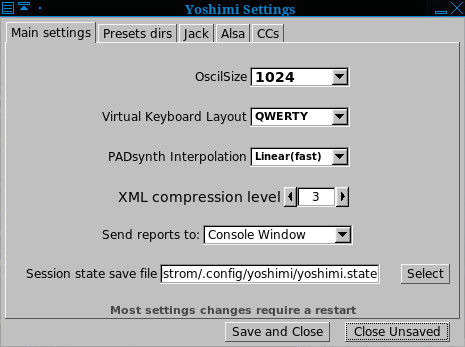
\includegraphics[scale=0.75]{menu/Yoshimi/yoshimi-settings-main.jpg}
   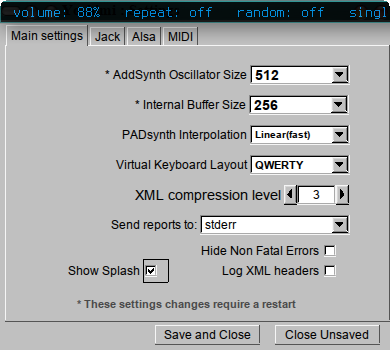
\includegraphics[scale=0.75]{1.3.9/yoshimi-settings-main.png}
   \caption{Yoshimi Main Settings Tab}
   \label{fig:yoshimi_main_settings_dialog}
\end{figure}

   The following settings exist in the \textsl{Main settings} tab:

   \begin{enumber}
      \item \textbf{AddSynth Oscillator Size} (was "OscilSize")
      \item \textbf{Internal Buffer Size} (new)
      \item \textbf{PADsynth interpolation}
      \item \textbf{Virtual Keyboard Layout}
      \item \textbf{XML compression level}
      \item \textbf{Send reports to}
      \item \textbf{Hide Non Fatal Errors}
      \item \textbf{Log XML headers}
      \item \textbf{Show Splash} (new)
      \item \textbf{Save and Close}
      \item \textbf{Close Unsaved}
   \end{enumber}

   \setcounter{ItemCounter}{0}      % Reset the ItemCounter for this list.

   \itempar{AddSynth Oscillator Size}{Main Settings!oscillator size}
   ADDsynth Oscillator Size (in samples).  This item used to be called
   "OscilSize".  Sets the number of the points of the ADDsynth oscillator.
   Bigger is better, but it takes more CPU time on the start of any note, and
   it may add latency to some processes.

   The default value for \textsl{Yoshimi} is shown marked with an asterisk,
   and the default value for \textsl{ZynAddSubFX} is 512.
   \index{asterisk}
   \index{default!asterisk}
   This asterisk/plus-sign convention is used throughout this manual.
   See \figureref{fig:yoshimi_oscilsize_values},
   shown below for the AddSynth Oscillator Size drop-down element.

   Values: \texttt{256, 512*, 1024, 2048, 4096, 8192, 16384}

\begin{figure}[H]
   \centering 
   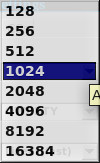
\includegraphics[scale=0.75]{menu/Yoshimi/main-oscilsize.jpg}
   \caption[OscilSize Values]{AddSynth Oscillator Size (samples)}
   \label{fig:yoshimi_oscilsize_values}
\end{figure}

   \itempar{Internal Buffer Size}{Main Settings!buffer size}
   This is a new item for version 1.3.6.  It is actually the old
   \textbf{Period Size} field from the \textbf{Alsa} tab.
   It sets the granularity of the sound generation.
   To find out the internal delay in milliseconds, divide the
   buffer-size value by the sample-rate, then multiply the result by 1000:
   For example, \(256 / 44100 * 1000 = 5.8 ms\).

   The default internal buffer size has been reduced from 1024 to 256.  One
   gets better latency that way.  Almost all modern computers can run
   \textsl{Yoshimi} with the current default (smaller) buffer-size value, and
   many will do so at 64 frames (and even 16 frames!)
   without any special precautions.
   
   Note that, for ALSA, if the audio destination is "default",
   then ALSA decides on the buffer size (among other settings), and
   \textsl{Yoshimi} will set it's internal buffer size to match,
   which always seems to be 1024.

   Values: \texttt{64, 128, 256*, 512, 1024}

\begin{figure}[H]
   \centering 
   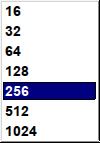
\includegraphics[scale=0.75]{menu/Yoshimi/main-internalsize.jpg}
   \caption[Internal Size Values]{AddSynth Internal Buffer Size (samples)}
   \label{fig:yoshimi_internalsize_values}
\end{figure}

   \itempar{PADsynth interpolation}{Main Settings!PADsynth Interpolation}
   See \figureref{fig:padsynth_interpolation}, shown below,
   for the interpolation values.
   From an email conversation with Paul Nasca, Will notes that
   the sound improvement with cubic interpolation is quite subtle, and requires
   a well designed audio setup, a PADsynth instrument with a fair amount of
   high-frequency content... and good hearing!

\begin{figure}[H]
   \centering 
   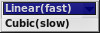
\includegraphics[scale=0.75]{menu/Yoshimi/main-padsynth-interpolation.jpg}
   \caption[PADSynth Interpolation]{PADSynth Interpolation Values}
   \label{fig:padsynth_interpolation}
\end{figure}

   Values: \texttt{Linear(fast)*, Cubic(slow)}

   \itempar{Virtual Keyboard Layout}{Main Settings!Virtual Keyboard Layout}
   The virtual keyboard is useful, but it is difficult to move the mouse
   rapidly to the next key on the virtual keyboard.
   Therefore, \textsl{Yoshimi} supports using the computer keyboard
   to produce notes.

\begin{figure}[H]
   \centering 
   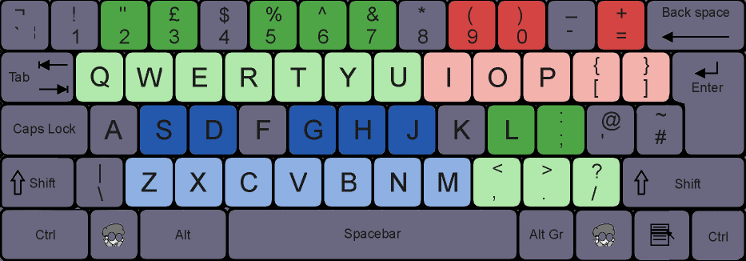
\includegraphics[scale=0.45]{top-panel/ascii-virtual-keyboard.png}
   \caption{QWERTY Virtual Keyboard Layout}
   \label{fig:qwerty_virtual_keyboard}
\end{figure}

   See \figureref{fig:qwerty_virtual_keyboard},
   for the mapping of the computer keyboard to the
   virtual keyboard.
   Three octaves (blue, green, and red) are available, with the dark keys of
   each color representing the "black" keys.
   Note that this is a QWERTY layout.  
   \textsl{Yoshimi} also supports other keyboard layouts.
   See \figureref{fig:virtual_kbd_layout},
   for the virtual keyboard layout settings drop-down.

   Values: \texttt{QWERTY*, Dvorak, QWERTZ, AZERTY}

\begin{figure}[H]
   \centering 
   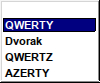
\includegraphics[scale=0.75]{menu/Yoshimi/main-virtual-kbd-layout.jpg}
   \caption[Virtual Keyboard Layout]{Virtual Keyboard Layout Values}
   \label{fig:virtual_kbd_layout} 
\end{figure}

   \itempar{XML compression level}{Main Settings!XML compression level}
   Gzip Compression level of \textsl{Yoshimi} XML files.
   The settings and instruments of
   \textsl{Yoshimi}
   are preserved in XML files.
   The value of 0 indicates that the XML file is uncompressed.

   In general, 0 is probably the best setting for debugging only.  Setting this
   option makes the XML files a bit larger, perhaps larger by a factor of more
   than 10, making a 10K file into a 180K file.  For a little "wasted" space
   and time, one can view the XML file in a text/programmer's editor.  But, if
   one's system is tight on disk space, higher levels of compression can be
   specified.  Using XML compression can also save file access time which may
   be beneficial if one's computer is borderline on latency.  This setting
   should stay at 3 if one is going to save large patchsets that will later be
   loaded while running. Uncompressing is \textsl{much} faster than file
   loading.

   Values: \texttt{0 to 9, 3*}

   \itempar{Send reports to}{Main Settings!Send Reports Destination}
   Notices and error messages can be sent to the standard error log of
   the terminal in which 
   \textsl{Yoshimi} can be run, or, more usefully, to
   an output console window.
   Now these messages are pushed in reverse order, to avoid scrolling
   and to make the most recent statuses easily visible.
   See \figureref{fig:send_reports_to}.
   It provides a depiction of the selection drop-down.

   Values: \texttt{stderr*, Console Window}

\begin{figure}[H]
   \centering 
   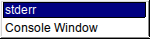
\includegraphics[scale=1.0]{menu/Yoshimi/main-send-reports-to.jpg}
   \caption[Send Reports]{Send Reports To}
   \label{fig:send_reports_to}
\end{figure}

   If the \textbf{Console Window} option is chosen, then the
   \textbf{Reports} button in the effects panel is enabled.
   Pressing the \textbf{Reports} button brings up a small console dialog, as
   shown in \figureref{fig:console_window}.

\begin{figure}[H]
   \centering 
   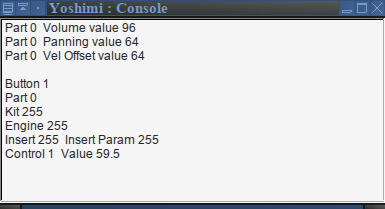
\includegraphics[scale=1.0]{1.3.9/console-window.png}
   \caption[Yoshimi Console Window]{Console Window}
   \label{fig:console_window}
\end{figure}

   \index{reports!middle-click}
   An interesting feature of the console window is that one can identify
   user-interface elements of the \textsl{Yoshimi} configuration in this window
   by a middle-click on the user-interface element.  The console window figure
   shows the results of middle-clicking on the following bottom-panel knobs in
   order:

   \begin{enumerate}
      \item Velocity Sense (left-click)
      \item Velocity Offset
      \item Pan
      \item Volume
   \end{enumerate}

   \index{reports!middle-click}
   Information about each knob middle-clicked is pushed to the top of the
   windows in reverse order.
   \index{reports!left-click}
   \index{reports!right-click}
   Information about an earlier left-click is shown at the bottom of the figure.
   Each left-click ("Button 1") will increase the parameter represented by the
   knob, and each right-click ("Button3") will decrease the parameter
   represented by the knob, and each change is reported in the console window.
   And, of course, each middle-click changes nothing, but reports the current
   value in the console window.
   This powerful feature provides a way to gather the information needed to
   control the parameter from the command-line.
   The output can be selected, copied, and pasted to a script or archive text
   file for safe-keeping.
   \index{MIDI learn}
   Consider it a form of "MIDI learn" that will be developed in the future.
   And note that it applies to output to \texttt{stderr} as well.

   \itempar{Hide Non Fatal Errors}{Main Settings!Hide Non-Fatal Errors}
   Especially when running from the command line (with reports going there
   too), under some circumstances one can get a swamp of low-level error
   messages (such as XRUNs) that is so large that one cannot work out what is
   going on. This feature disables these error messages; it is a work in
   progress to catch the bulk of them, while still reporting top-level messages
   and ones that cause a forced exit (surely not!)

   \itempar{Log XML headers}{Main Settings!Log XML headers}
   This item sends the information to the console window
   (or \texttt{stderr}) so that
   one can then see what \textsl{ynAddSubFX}/\textsl{Yoshimi}
   version created the file.

   \itempar{Show Splash}{Main Settings!Show Splash}
   This item will speed up the start-up of \textsl{Yoshimi} slightly
   if unchecked, by not showing the splash screen while files are being loaded.

\paragraph{Menu / Yoshimi / Settings / Jack}
\label{paragraph:menu_yoshimi_settings_jack}

   JACK is the "Jack Audio Connection Kit", very useful for increasing audio
   performance and configurability.
   When using the JACK audio backend, instruments can be individually routed
   and sent to the main L/R outputs. This is controlled from the
   panel window,
   \sectionref{subsec:mixer_panel_window},
   and the settings are saved with all the other parameters.

   Direct part outputs carry the Part and Insertion effects, but not the
   System ones.

\begin{figure}[H]
   \centering 
%  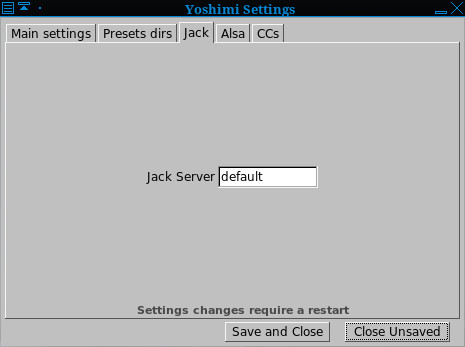
\includegraphics[scale=0.75]{menu/Yoshimi/yoshimi-settings-jack.jpg}
%  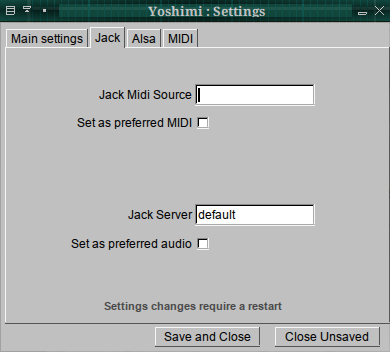
\includegraphics[scale=0.75]{1.3.8/yoshimi-settings-jack.jpg}
   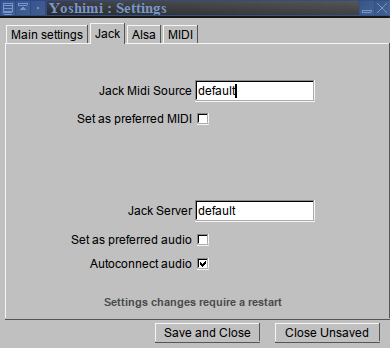
\includegraphics[scale=0.75]{1.3.9/yoshimi-settings-jack.png}
   \caption[JACK Settings]{JACK Settings Dialog}
   \label{fig:yoshimi_settings_jack}
\end{figure}

   The following items are provided by the Jack settings:

   \begin{enumber}
      \item \textbf{Jack Midi Source}
      \item \textbf{Set as preferred MIDI}
      \item \textbf{Jack Server}
      \item \textbf{Set as preferred audio}
      \item \textbf{Autoconnect audio} (new, 1.3.9)
      \item \textbf{Save and Close}
      \item \textbf{Close Unsaved}
   \end{enumber}

   \setcounter{ItemCounter}{0}      % Reset the ItemCounter for this list.

   \itempar{Jack Midi Source}{JACK!MIDI source}
   Jack MIDI Source.
   It is possible to have more than one JACK MIDI source.  This option
   tells this instance of \textsl{Yoshimi} which JACK
   client to try to auto-connect to for MIDI input.
   This option corresponds to the \textsl{Yoshimi} command line option
   \texttt{--jack-midi(=device)}.

   Values: \texttt{default*, name} name, as in "jackd --name"

   \itempar{Set as preferred MIDI}{JACK!set as preferred MIDI}
   Set as preferred MIDI for JACK.
   This setting determines which MIDI connections a particular instance will
   first attempt. The switches are mutually exclusive across JACK and ALSA,
   so if one checks ALSA for MIDI, it automatically unchecks JACK for MIDI.
   As well as from the GUI, this setting can be set (for instance 0) from the
   command line, both at start-up and once running.

   \itempar{Jack Server}{JACK!server name}
   Jack Server Name.
   It is possible to have more than one JACK server running.  This option
   tells this instance of \textsl{Yoshimi} which JACK server to use.
   This option corresponds to the \textsl{Yoshimi} command line option
   \texttt{--jack-audio(=server)}.

   Values: \texttt{default*, name} name, as in
   \texttt{jackd --name}.

   \itempar{Set as preferred audio}{JACK!set as preferred audio}
   Set as preferred audio for JACK.
   This setting determines which audio connections a particular instance will
   first attempt. The switches are mutually exclusive across JACK and ALSA,
   so if one checks ALSA for audio, it automatically unchecks JACK for audio.
   As well as from the GUI, this setting can be set (for instance 0) from the
   command line, both at start-up and once running.
   Note that any of these setting changes require a restart of \textsl{Yoshimi}
   to take effect.

   \itempar{Autoconnect audio}{JACK!autoconnect audio}
   Sets \textsl{Yoshimi} to connect automatically to the JACK server, just like
   the \texttt{-K} command-line option does.  (However, note that the
   command-line has no way to disable this feature it the configuration has been
   saved.)

\paragraph{Menu / Yoshimi / Settings / ALSA}
\label{paragraph:menu_yoshimi_settings_alsa}

   A significant improvement is to the handling of ALSA audio, which is still
   very important for some people. Until now, \textsl{Yoshimi} has insisted
   on a 2-channel, 16-bit format. Tests have shown that virtually all
   motherboard sound chipsets will handle this, but many external ones don't.

   From \textsl{Yoshimi} 1.3.6 onwards, when using ALSA audio,
   \textsl{Yoshimi} first tries to connect 2 channels at 32 bit depth.  If
   that connection does not succeed, then \textsl{Yoshimi} negotiates
   whatever the soundcard will support.  For example, a card might support
   only 24 bits, and 6 channels.  So \textsl{Yoshimi} will fall back to
   24 bit, and, due to its own limits, will use only channels 1 and 2.
   With external sound modules in mind, endian swaps are also implemented.

   To be able to reliably use ALSA audio, one needs to set a card name, not just
   "Default".  In a terminal window enter the following command:

   \begin{verbatim}
      $ cat /proc/asound/card*/id
   \end{verbatim}

   The result of this command should be something like:

   \begin{verbatim}
      PCH
      K6
   \end{verbatim}

   Go to the ALSA settings tab illustrated below, and in 
   \textsl{Alsa Audio Device} enter, for example, "hw:PCH".
   This ensures one will always connect to this card at startup regardless of
   the order this and other ones.  Another benefit of using this hardware name
   is that ALSA will now use \textsl{Yoshimi}'s internal
   buffer size (256), otherwise ALSA will force \textsl{Yoshimi} to accept its
   default size (usually 1024).

   One can also set the sample rate, but bear in mind that not all cards can use
   all of these.  The sample rates 44100 and 48000 are almost always available.
   If one sets a Midi Device as well (such as a keyboard) Yoshimi will try to
   find and connect to this device at startup.

   To find the MIDI devices available, try:

   \begin{verbatim}
      $ grep Client /proc/asound/seq/clients
   \end{verbatim}

   The result of this command should be something like:

   \begin{verbatim}
      Client info
      Client   0 : "System" [Kernel]
      Client  14 : "Midi Through" [Kernel]
      Client 128 : "TiMidity" [User]
   \end{verbatim}

   It is not obvious how ALSA audio is controlled and who takes command.  If
   one sets a specific audio destination, then \textsl{Yoshimi} makes a
   request.  It's often a negotiation on bit depth and channel count, but
   \textsl{Yoshimi} nearly always gets to decide the buffer size, which is the
   internal buffer size.  However, if the destination is 'default' then ALSA
   decides on the sound card, bit depth, number of channels and the buffer
   size, and \textsl{Yoshimi} will set it's internal buffer size to match.  On
   most machines this seems to be 1024.

\begin{figure}[H]
   \centering 
%  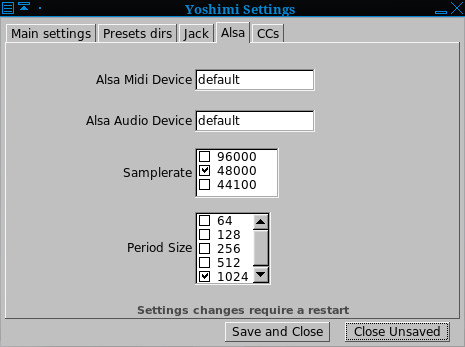
\includegraphics[scale=0.75]{menu/Yoshimi/yoshimi-settings-alsa.jpg}
   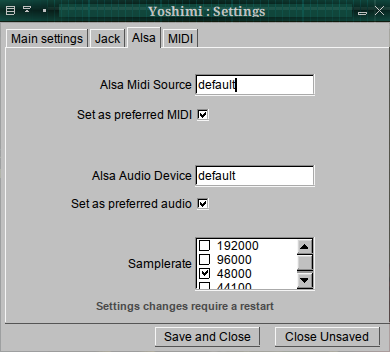
\includegraphics[scale=0.75]{1.3.8/yoshimi-settings-alsa.png}
   \caption[ALSA Settings]{ALSA Settings Dialog}
   \label{fig:yoshimi_settings_alsa}
\end{figure}

   \setcounter{ItemCounter}{0}      % Reset the ItemCounter for this list.

   \itempar{Alsa Midi Source}{ALSA!MIDI Source}
   ALSA MIDI Source.
   The purpose of this setting is the same as the command line option
   \texttt{--alsa-midi="name"}.
   It is used so that \textsl{Yoshimi} can auto connect to a MIDI source
   such as a keyboard.  For example, the one that Will has identifies itself
   as name = "Hua Xing".
   A port name, such as "128:0" (for one of the ports provided by
   \textsl{TiMidity}) should work as well.
   If the destination is "default",
   then ALSA decides on the sound card, bit depth, number of channels and the
   buffer size, and \textsl{Yoshimi} will set it's internal buffer size to
   match.  On most machines this always seems to be 1024.

   Values: \texttt{default*}

   \itempar{Set as preferred MIDI}{ALSA!Set as preferred MIDI}
   Set as preferred MIDI for ALSA.
   This setting determines which MIDI connections a particular instance will
   first attempt. The switches are mutually exclusive across JACK and ALSA,
   so if one checks ALSA for MIDI, it automatically unchecks JACK for MIDI.
   As well as from the GUI, this setting can be set (for instance 0) from the
   command line, both at start-up and once running.

   \itempar{Alsa Audio Device}{ALSA!audio device}
   ALSA Audio Device.
   This specifies the sound card to which \textsl{Yoshimi} can connect.
   Normally, this will be an ALSA hardware specification such as
   "hw:0".
   ALSA audio also lets one connect to a sound card by name. For example,
   with a Komplete Audio KA 6 sound card, the device specification is
   "hw:K6". This feature is particularly useful for USB modules, as one can
   never be sure where they appear numerically.

   Values: \texttt{default*}

   \itempar{Set as preferred audio}{ALSA!Set as preferred audio}
   Set as preferred audio for ALSA.
   This setting determines which audio connections a particular instance will
   first attempt. The switches are mutually exclusive across JACK and ALSA,
   so if one checks ALSA for audio, it automatically unchecks JACK for audio.
   As well as from the GUI, this setting can be set (for instance 0) from the
   command line, both at start-up and once running.

   \itempar{Samplerate}{ALSA!sample rate}
   Sample Rate.
   Sets the quality of the sound, higher is better, but it uses more CPU.  One
   can select from a list.  Note that both ALSA and JACK will support the
   192000 rate, if the sound-card supports it.  To find out the internal delay
   in milliseconds, divide the buffer-size value by the Sample Rate and
   multiply the result by 1000 (256 / 44100 * 1000 = 5.8 ms).

   Note that, as of version 1.3.6, the \textbf{Period Size} field has been
   removed from the \textbf{Alsa} tab, and is replaced by the 
   \textbf{Internal Buffer Size} field in the \textbf{Main Settings} tab.
   Note that any of these setting changes require a restart of \textsl{Yoshimi}
   to take effect.
   
   \textsl{ZynAddSubFX}: if one wants a sample-rate that
   is not in the list, select "Custom" and change the value from the right.
   Default is 44100.

   Values: \texttt{192000, 96000, 48000*, 44100}

\paragraph{Menu / Yoshimi / Settings / MIDI}
\label{paragraph:menu_yoshimi_settings_ccs}

   The CC settings tab has been renamed the "MIDI" tab.
   This tab, shown in
   \figureref{fig:yoshimi_settings_cc},
   presents MIDI bank-root, bank, program change, and extended program
   change settings, plus some new values.

   A new feature as of version 1.3.6 is that some changes to the items in this
   tab cause a red \textbf{Pending} button to appear.  Pressing this
   button saves that particular change.

\begin{figure}[H]
   \centering 
%  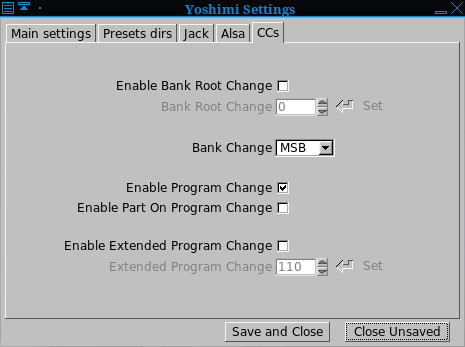
\includegraphics[scale=0.75]{menu/Yoshimi/yoshimi-settings-ccs.jpg}
%  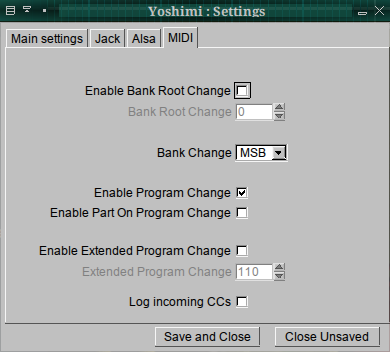
\includegraphics[scale=0.75]{1.3.8/yoshimi-settings-midi.png}
   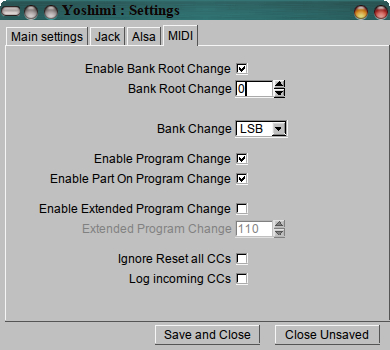
\includegraphics[scale=0.75]{1.3.9/yoshimi-settings-ccs.jpg}
   \caption[MIDI Preferences]{MIDI Preferences}
   \label{fig:yoshimi_settings_cc}
\end{figure}

%  TODO:  Could add a figure showing the red Pending button.

   The following items are provided by the MIDI settings tab:

   \begin{enumber}
      \item \textbf{Enable Bank Root Change}
      \item \textbf{Bank Root Change}
      \item \textbf{Bank Change}
      \item \textbf{Enable Program Change}
      \item \textbf{Enable Part On Program Change}
      \item \textbf{Enable Extended Program Change}
      \item \textbf{Extended Program Change}
      \item \textbf{Ignore Reset all CCs}
      \item \textbf{Log incoming CCs}
      \item \textbf{Save and Close}
      \item \textbf{Close Unsaved}
   \end{enumber}

   \setcounter{ItemCounter}{0}      % Reset the ItemCounter for this list.

   The concepts of banks and roots is very useful.
   See \sectionref{subsec:concepts_banks_and_roots}.
   The settings in this tab affect the usage of banks and root changes
   controlled by MIDI messages, thereby making \textsl{Yoshimi} able to
   implement MIDI automation.

   \itempar{Enable Bank Root Change}{MIDI preferences!enable bank root change}
   Enable Bank Root Change.

   Values: \texttt{Off*, On}

   \itempar{Bank Root Change}{MIDI preferences!bank root change}

   Values: \texttt{0*, to 127}

   If enabled, a new reddish button, \textbf{Pending}, appears.
   Once the change has been made in the scroll list, click this button
   to set the change.
   \textbf{Warning:}
   The \textbf{Save and Close} button will not result in the removal of the
   \textbf{Pending} button.
   This result seems counter-intuitive, but the pending button is not removed
   here because, at that point, it still hasn't actually been either set or
   abandoned. It remains available for when the user actually makes up his/her
   mind.

   \itempar{Bank Change}{MIDI preferences!bank change}
   Bank Change.
   Defines which MIDI preferences one wants to use.
   Note that MIDI Controller 0 = CC0 = Bank Select MSB, and MIDI Controller
   32 = CC32 = Bank Select LSB.
   When combined, these Bank Select messages provide \[128*128 = 16384\]
   banks.

   But note that all a Bank Select does is selects the bank for the next
   Program Change event.  The program doesn't change after changing a bank,
   until a Program Change is sent.

   Bank changes can be completely disabled; some hardware
   synthesizers don't play nice with banks.

   Values: \texttt{LSB, MSB*, Off}

   \itempar{Enable Program Change}{MIDI preferences!enable program change}

   Values: \texttt{Off*, On}

   Enables/disables MIDI program change.
   Program changes can be completely disabled, but some hardware synths don't
   play nice!

   \itempar{Enable Part On Program Change}{MIDI preferences!enable part change}

   Values: \texttt{Off*, On}

   The part is automatically enabled if the MIDI program was changed on this
   part.

   \itempar{Enable Extended Program Change}{MIDI preferences!enable extended program change}

   Values: \texttt{Off*, On}

   \itempar{Extended Program Change}{MIDI preferences!extended change}
   If enabled, a new reddish button, \textbf{Pending}, appears.
   Once the change has been made in the scroll list, click this button
   to set the change.

   Values: \texttt{0-127, 110*}

   \itempar{Ignore Reset all CCs}{MIDI preferences!Ignore Reset all CCs}
   Causes \textsl{Yoshimi} to ignore this message.
   \index{CC monitor}
   For example, using \textsl{Yoshimi}'s fairly new CC monitor (see the next
   item), Will found that \textsl{Rosegarden} was sending CC 121 (reset all
   controllers) at the start of some song segments.  Checking this option
   prevents unwanted resets.

   Values: \texttt{Off*, On}

   \itempar{Log incoming CCs}{MIDI preferences!Log incoming CCs}
   This setting is is about the only setting that is never saved. It is there
   solely as an aid for when \textsl{Yoshimi} appears to ignore MIDI commands,
   as it tells one exactly what \textsl{Yoshimi} thinks it received.

   Values: \texttt{Off*, On}

\subsubsection{Menu / Yoshimi / Exit}
\label{subsubsec:menu_yoshimi_exit}

   Simply exits from \textsl{Yoshimi}.
   The user is prompted if unsaved changes exist, as shown in
   \figureref{fig:yoshimi_change_exit}.

   One can sometimes get a false parameters-changed warning if one
   scrolls through one of the menu type entries without actually changing it.
   Better safe than sorry!

\begin{figure}[H]
   \centering 
   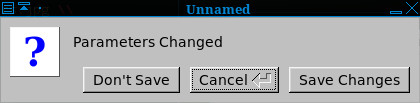
\includegraphics[scale=0.75]{menu/Yoshimi/yoshimi-menu-exit-parameters-changed.jpg}
   \caption[Yoshimi Menu, Exit]{Yoshimi Menu, Exit}
   \label{fig:yoshimi_change_exit}
\end{figure}

% We moved some out-of-date menu entries into the following document, and
% created additional sub-sections to include, with up-to-date information.
%
% %-------------------------------------------------------------------------------
% yum_menu
%-------------------------------------------------------------------------------
%
% \file        yum_menu_instruments.tex
% \library     Documents
% \author      Chris Ahlstrom
% \date        2015-05-11
% \update      2016-02-27
% \version     $Revision$
% \license     $XPC_GPL_LICENSE$
%
%     Provides the Menu section of yoshimi-user-manual.tex.
%
%-------------------------------------------------------------------------------

\subsection{Menu / Instruments}
\label{subsec:menu_instrument}

   The \textsl{Yoshimi} Instruments menu lets one select instruments and work
   with banks of instruments.
   \textsl{Yoshimi} stamps instrument XML files with its own major and minor
   version numbers so it is possible to tell which version created the files,
   or whether they were created by \textsl{ZynAddSubFX}.

   When opening an instrument bank one can now tell exactly which synth engines
   are used by each instrument. This is represented by three pale background
   colours:

   \begin{itemize}
      \item \textcolor{red}{Red}: ADDsynth
      \item \textcolor{blue}{Blue}: SUBsynth
      \item \textcolor{green}{Green}: PADsynth
   \end{itemize}

   These new colored engine backgrounds aren't just pretty. They give real
   information about expected processor load, and time taken to be ready when
   loaded:

   \begin{itemize}
      \item \textsl{Processor Load, low to high}: PAD, SUB, then ADD.
      \item \textsl{Time to initialize, low to high}: SUB, ADD, PAD.
   \end{itemize}

   If the instruments are kits they scanned to find out if 
   \textsl{any} member of the kit contains each engine.
   This scanning is duplicated in the current part, the mixer panel for the
   currently loaded instruments, and in the Instrument Edit window the same
   colors highlight the engine names when they are enabled with the check
   boxes. 

   The following sub-menus are provided, as shown in
   \figureref{fig:yoshimi_instrument_menu}.

\begin{figure}[H]
   \centering 
   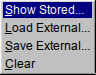
\includegraphics[scale=1.0]{1.3.8/yoshimi-menu-instrument.jpg}
   \caption{Yoshimi Menu, Instrument}
   \label{fig:yoshimi_instrument_menu}
\end{figure}

   TODO:  Document the many differences in 1.3.8 here.

   \begin{enumber}
      \item \textbf{Clear Instrument...}
      \item \textbf{Open Instrument...}
      \item \textbf{Save Instrument...}
      \item \textbf{Show Instruments...}
      \item \textbf{Show Banks...}
      \item \textbf{Show Root Paths...}
   \end{enumber}

   These menu entries don't appear in the order in which they would normally
   be used.  For simplicity, it is better, especially for \textsl{Yoshimi}
   1.3.5 and above, to summarize how to navigate through these menu items,
   before showing each one in detail.

   \setcounter{ItemCounter}{0}      % Reset the ItemCounter for this list.

   \itempar{Set Current Root Path}{root!set current}
   \index{root!current}
   Instruments are stored in banks, and banks are stored in root directories,
   also known as "roots".  In \textsl{Yoshimi}, there can be a number of
   roots that exist in a user's directory structure, but only one root can be
   the current root.  Thus, the first step is to set up the current root
   directory to point to where we have stored all our banks of instruments.

   \begin{enumber}
      \item In \textsl{Yoshimi}, navigate to the \textbf{Instrument / Show
      Root Paths...} entry in the main menu.
      \item In the \textbf{Bank Root Paths} dialog, select the desired
      bank path by clicking on it.
      \item Click the \textbf{Make Current} button.
%     \item Then click the \textbf{Open Current} button.
      \item Then click the \textbf{Save and Close} button.
   \end{enumber}

   For example, one can make the \texttt{/usr/share/yoshimi/banks} directory
   the current root directory.  This directory is the default location for
   banks when \textsl{Yoshimi} is first installed.
   In the following figure, we set it to the author's local directory,
   \texttt{~/Audio/yoshimi/banks}.
   In general, it is recommended that one copies the default installed
   directories to a local directory, in order to be able to work with them,
   making additions and changes without needing root permissions, and
   without risking the corruption of the default installation.

   For figures and details about the \textbf{Show Root Paths...} menu entry,
   see \sectionref{subsubsec:menu_instrument_show_root_paths}.

   \itempar{Show Current Bank Set}{banks!show}
   Once the current root has been set, one can then see all of the banks
   under that root.  Navigate to the \textbf{Instrument / Show Banks...} menu
   entry and click it.  This brings up a dialog such as the one shown in
   \figureref{fig:show_ca_banks}.  That dialog shows all of the banks that
   exist in the current root directory.  Each is auto-numbered by
   \textsl{Yoshimi} the first time that root directory is accessed, and the
   current bank is highlighted in pink.

   Clicking on a bank with both make that bank the current bank, and opens an
   instruments dialog, such as that shown in
   \figureref{fig:show_alex_j_bank}.

   \itempar{Show Instruments in Current Bank}{instruments!show}
   Once the current root and current bank have been set, another way to show
   the instruments is to navigate to the
   \textbf{Instrument / Show Instruments...} menu entry and click on it.
   Again, this action opens an instruments dialog, such as that shown in
   \figureref{fig:show_alex_j_bank}.

   A left-click on a particular instrument sets that instrument into the
   current Part in force in the main \textsl{Yoshimi} window, where it can
   then be edited, if desired.

   \index{anti-auto-clutter}
   Right-clicking on an instrument causes the instruments list dialog
   to disappear, and be replaced by an instrument dialog.  While this
   behavior might be surprising, it is part of the anti-auto-clutter feature
   of \textsl{Yoshimi}.

   Now that we know how to easily navigate through roots, banks, and
   instruments, we can discuss each of the \textbf{Instrument} menu entries
   in detail.

\subsubsection{Menu / Instrument / Clear Instrument...}
\label{subsubsec:menu_instrument_clear}

   This menu entry brings up a prompt to clear the parameters of the
   instrument that is currently loaded in the current part.

\begin{figure}[H]
   \centering 
   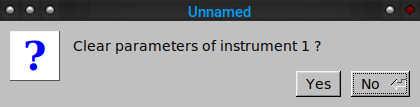
\includegraphics[scale=0.75]{menu/Instrument/clear-instrument.jpg}
   \caption{Clear Instrument Dialog}
   \label{fig:clear_instrument_dialog}
\end{figure}

   \textbf{Bug:}
   \index{bugs!need to clear instrument?}
   Sometime it seems that one needs to clear the instrument if one is
   loading a new instrument to test it out, because some settings seem
   to remain from the previous instrument.

   \textsl{Don't quote us on that.  Maybe Will has fixed that issue by now.}

\subsubsection{Menu / Instrument / Open Instrument...}
\label{subsubsec:menu_instrument_open}

   This menu entry brings up a prompt to open a new instrument.
   This prompt is a file-dialog, and it doesn't depend at all on the settings
   of the current root or the current bank.  It does have a
   \textbf{Favorites} button to help the user get quickly to the desired
   location of instrument files.

\begin{figure}[H]
   \centering 
   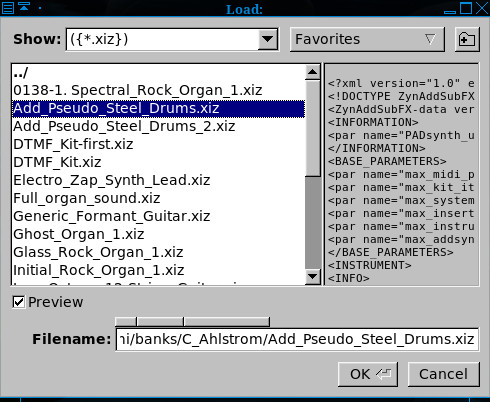
\includegraphics[scale=0.75]{menu/Instrument/open-instrument.jpg}
   \caption{Open Instrument Dialog}
   \label{fig:open_instrument_dialog}
\end{figure}

   This dialog has a number of user-interface elements to discuss.

   \begin{enumber}
      \item \textbf{Show}
      \item \textbf{Favorites}
      \item \textbf{Create a new diretory}
      \item \textbf{Instrument List}
      \item \textbf{XML Preview}
      \item \textbf{Preview}
      \item \textbf{Show hidden files}
      \item \textbf{Directory Bar}
      \item \textbf{Filename}
      \item \textbf{OK}
      \item \textbf{Cancel}
   \end{enumber}

   \setcounter{ItemCounter}{0}      % Reset the ItemCounter for this list.

   \itempar{Show}{Open Instrument!show}
   Show types of files.
   This item shows a file filter for selecting instrument files.
   The types of filters are as follows (screen shot not available):

   \begin{enumber}
      \item \textbf{(\{*.xiz\})} (compressed XML files)
      \item \textbf{All Files (*)}
      \item \textbf{Custom Filter}
   \end{enumber}

   \itempar{Favorites}{Open Instrument!favorites}
   Favorite directories.
   Provides a list of options and favorite directories in which to find 
   instrument files.

\begin{figure}[H]
   \centering 
   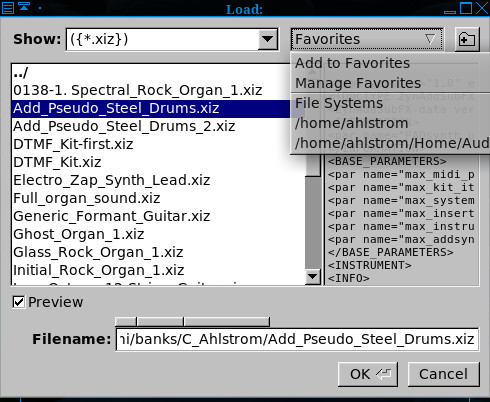
\includegraphics[scale=0.75]{menu/Instrument/favorites-dropdown.jpg}
   \caption{Favorites Drop-down}
   \label{fig:open_instrument_favorites}
\end{figure}

   \begin{enumber}
      \item \textbf{Add to Favorites}
      \item \textbf{Manage Favorites}
      \item \textbf{File Systems}
      \item \textbf{(Additional favorite directories)}
   \end{enumber}

   \index{Add to Favorites}
   \textbf{Add to Favorites}
   simply adds the currently selected directory shown in the instrument list
   to the list of favorites.

   To add Favorites in the file dialog, navigate to the desired directory.
   Then click \textbf{Favorites}, and select \textbf{Add to Favorites}.

   Once one has a number of favorites set up,
   there is a \textbf{Manage Favorites} that can be used.
   For example, if one needs to get rid of a directory, one can use the
   \textbf{Manage Favorites}
   \index{Manage Favorites}
   dialog, shown in
   \figureref{fig:manage_instrument_favorites} below,
   to do that.

\begin{figure}[H]
   \centering 
   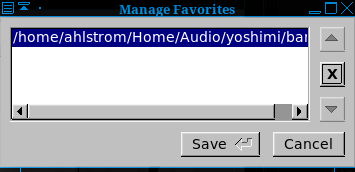
\includegraphics[scale=1.0]{menu/Instrument/manage-favorites.png}
   \caption{Favorites Drop-down}
   \label{fig:manage_instrument_favorites}
\end{figure}

   \textbf{File Systems} \index{File Systems}
   Provides a list of all file systems starting at root ("\texttt{/}").
   This list can be pretty confusing, with a lot of entries.
   But note that one navigates to ("\texttt{/}"), and from there to
   \texttt{/usr/share/yoshimi/banks} to get easy access to all the
   instruments that are preinstalled with
   \textsl{Yoshimi}.
   Generally, one will want to use only
   \textbf{Add to Favorites} and \textbf{Manage Favorites}.

   \itempar{Create Directory}{Open Instrument!create new directory}
   Creates a New Directory.
   This little symbol options a small "New Directory?" dialog (not shown
   here, it is very simple and stock) into which one can type a directory
   name to be added to the current directory of the instrument list.

   \itempar{Instrument List}{Open Instrument!instrument list}
   Provides a list of the instrument files available in the current
   directory.  Also shown are sub-directories (if available)
   that might contain more instruments, and a ("\texttt{../}") entry
   to navigate to the parent directory.

   \itempar{Preview}{Open Instrument!preview checkbox}
   If one thinks the preview feature is not useful, uncheck this check-box.
   so that one doesn't see the preview window.  As a bonus, one can see more
   of the instrument file-name.

   \itempar{Preview pane}{Open Instrument!preview pane}
   XML Preview.
   This box can show the beginning of the XML data of an instrument file.
   \textbf{Bug:}
   \index{bugs!compressed XML preview}
   It seems to show the XML only if the XML is not compressed.

   \itempar{Show hidden files}{Open Instrument!show hidden files}
   Shows file that are hidden.  Not sure how useful this feature is;
   who would hide a \textsl{Yoshimi} instrument file?

   \itempar{Directory Bar}{Open Instrument!directory bar}
   Provides an alternate way to move up through the directory structure.

   \itempar{Filename}{Open Instrument!filename}
   File Name.
   Provides the full path to the instrument file.

   \itempar{OK/Cancel}{Open Instrument!ok/cancel}
   We don't really need to discuss the \textbf{OK} and \textbf{Cancel}
   buttons, do we?

\subsubsection{Menu / Instrument / Save Instrument...}
\label{subsubsec:menu_instrument_save}

   This menu entry brings up a prompt to save a new instrument within the
   user's file system.
   It has all of the user-interface elements of the "Open Instrument"
   dialog shown in
   \figureref{fig:open_instrument_dialog}
   in \sectionref{subsubsec:menu_instrument_open}.
   Like that dialog, it is not dependent on the current root or current bank.
   However, if nothing has changed, then a "Nothing to Save!" prompt (not
   pictured) is shown.

   With \textsl{ZynAddsubFX} and older versions of \textsl{Yoshimi},
   it was possibly to end up with unnamed instruments. Since version
   1.3.4, \textsl{Yoshimi} will trap such an occurrence and name it
   'No Title'; it will not let one save the unedited default sound.

\subsubsection{Menu / Instrument / Show Instruments...}
\label{subsubsec:menu_instrument_show}

   Instruments are stored in banks. The banks (and current bank setting)
   are loaded/saved
   automatically by the program, so one doesn't have to worry about saving the
   banks before the program exits. On program start, the last used bank is
   loaded. A single bank can store up to 128 instruments. 
   However, there is space for a number of additional
   instruments in the bank, the extended-program section, to allow up to 160
   instruments in a bank.

   When the \textbf{Show Instruments...} button is selected, a dialog comes
   up that shows all of the instruments present in the currently-selected
   bank.
   
\begin{figure}[H]
   \centering 
   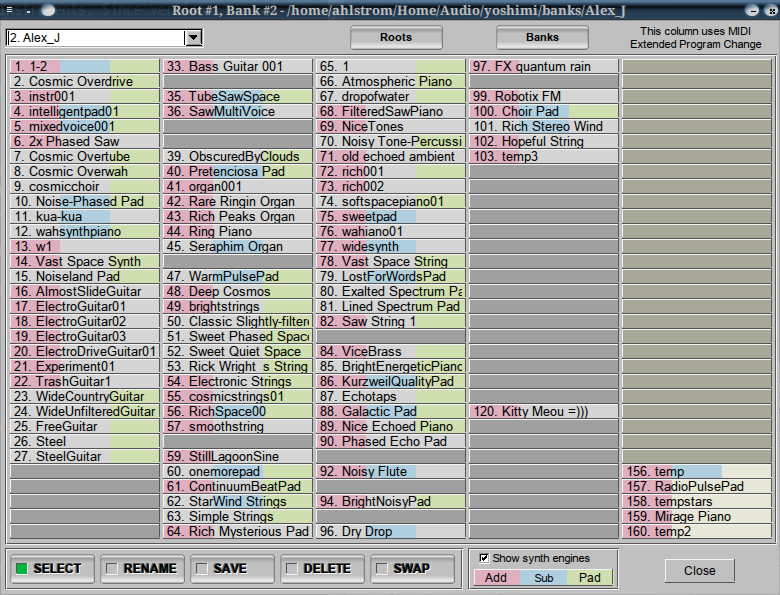
\includegraphics[scale=0.75]{1.3.6/Alex_J_bank_instruments.png}
   \caption[Instruments in Current Bank]{Instruments in Current Bank 1.3.6}
   \label{fig:show_alex_j_bank}
\end{figure}

   As \figureref{fig:show_alex_j_bank}
   shows, this is a very complex dialog with a lot of options.
   Note how \textsl{Yoshimi} now shows the color codings for the
   synth-sections used in each instrument:
   red for ADDsynth, blue for SUBsynth, and
   green for PADsynth.

   Also note how the numbers at the beginning of the filenames are used as
   an "instrument" or "program" number.  These numbers can be used in MIDI
   Program Change commands.
   
   All of the files with filenames starting with 4-digit numbers will be
   shown in the slot corresponding number.  Those without numbers will start
   with numbers at 129 or above ("extended program change").  One should give
   them numbers by renaming them outside of \textsl{Yoshimi}, then reloading
   the bank.

   \index{extended program}
   Note that MIDI CC
   (see \sectionref{paragraph:menu_yoshimi_settings_ccs})
   can be set to access voices from 129 to 160.
   All the Bank controls in the \textbf{MIDI} settings tab take immediate
   effect when set.
   Bank and program changes can be completely disabled in the settings tab;
   some hardware synths don't play nice with it.

   Learning how to use the Instruments dialog is an important way to make
   instruments easier to manage, and so this will be a long discussion.

%  An important pair of concepts in \textsl{Yoshimi} are
%  \textsl{banks} and \textsl{roots}.  These concepts are described in
%  \sectionref{subsec:concepts_banks_and_roots}.

%  A bank has 3 modes in \textsl{ZynAddSubFX}: 

%  \begin{enumber}
%     \item \textbf{READ}.
%        The instrument is loaded from the bank to the current part.
%     \item \textbf{WRITE}.
%        The instrument is written to the bank.
%     \item \textbf{CLEAR}.
%        The instrument from the bank is cleared (removed).
%  \end{enumber}

%  Pressing the left mouse button on a slot reads/writes/clears the
%  instrument from/to it (according to the current mode).
   
%  Pressing the right mouse button on a slot changes its name.

%  The setup in \textsl{Yoshimi} is a bit different than in
%  \textsl{ZynAddSubFX}.
%  Observe \figureref{fig:show_ca_bank}.
%  It shows a bank loaded from a directory containing customs
%  banks from one of the authors of this document.

   Note that this dialog has been modified in recent versions of
   \textsl{Yoshimi}.

   Here is a list of the user-interface items in the instruments/banks dialog.

   \begin{enumber}
      \item \textbf{Bank Names}
      \item \textbf{Roots}
      \item \textbf{Banks}
      \item \textbf{Instrument and Bank Matrix}
      \item \textbf{SELECT}
      \item \textbf{RENAME}
      \item \textbf{SAVE}
      \item \textbf{DELETE}
      \item \textbf{SWAP}
      \item \textbf{Show synth engines}
         (was \textbf{Show PADsynth status})
      \item \textbf{Close}
   \end{enumber}

   \setcounter{ItemCounter}{0}      % Reset the ItemCounter for this list.

   \itempar{Bank Names}{instruments!bank names}
   Instruments Bank Name.
   Basically, each bank is a directory name, with a number prepended.
   The banks are found under the current root, which is a also a directory
   name, and is the name of the parent directory of a set of banks.
   Here is the Bank Names drop-down list for "my" setup, which has the
   default banks plus a lot of banks found around the Internet:

\begin{figure}[H]
   \centering 
   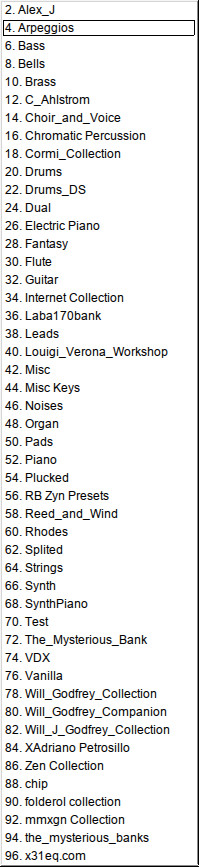
\includegraphics[scale=0.75]{menu/Instrument/bank-list.jpg}
   \caption[A Sample Bank List]{A Sample Bank List}
   \label{fig:bank_list}
\end{figure}

   And here is the directory listing associated with it, in the order
   produced by the UNIX/Linux "ls -1" (list single-column) command (shown in
   two columns to save space):

   \begin{verbatim}
      Alex_J                        Noises
      Arpeggios                     Organ
      Bass                          Pads
   '  Bells                         Piano
      Brass                         Plucked
      C_Ahlstrom                    RB Zyn Presets
      chip                          README
      Choir_and_Voice               Reed_and_Wind
      Chromatic Percussion          Rhodes
      Cormi_Collection              Splited
      Drums                         Strings
      Drums_DS                      Synth
      Dual                          SynthPiano
      Electric Piano                Test
      Fantasy                       The_Mysterious_Bank
      Flute                         the_mysterious_banks
      folderol collection           Vanilla
      Guitar                        VDX
      Internet Collection           Will_Godfrey_Collection
      Laba170bank                   Will_Godfrey_Companion
      Leads                         Will_J_Godfrey_Collection
      Louigi_Verona_Workshop        x31eq.com
      Misc                          XAdriano Petrosillo
      Misc Keys                     Zen Collection
      mmxgn Collection
   \end{verbatim}

   The first thing to note is that there are only 128 \textsl{Yoshimi} banks
   supported in a \textsl{Yoshimi} root.  The list above takes up about half
   of the available slots, so it might be time to move some of those banks
   to a new root directory.

   The numbers in the drop-down list are generated by \textsl{Yoshimi} the
   first time it sees a new root path or a new bank within the root path.
   Once set, these numbers will never change unless one actually moves them
   around (using the \textbf{SWAP} button).

   The bank number is also the MIDI ID for the bank;
   one can be sure that it will always
   be there for bank changes, no matter how many banks are added later.
   \textsl{Yoshimi} always lists the banks in ID order, not alphabetical
   order, so one can group them sensibly and permanently.
   However, at first-time creation \textsl{Yoshimi} sets the IDs in
   alphabetical order and tries to space them evenly over the range to
   provide some wiggle room.                                        

   Selecting one of the items in this drop-down list selects the bank and
   loads it into the Banks dialog.

   \index{anti-auto-clutter}
   Right-clicking on a bank causes the banks list dialog
   to disappear, and be replaced by the bank dialog.  While this
   behavior might be surprising, it is part of the anti-auto-clutter feature
   of \textsl{Yoshimi}.

   \itempar{Roots}{instruments!roots}
   Instruments Roots Button.
   Shows a list of directories that can serve as "root" directories.
   The "Bank Root Paths" dialog shown in
   \figureref{fig:show_banks_roots} shows
   the system root (e.g. \texttt{/usr/share/yoshimi/banks}) and
   a user's home location for his/her banks and roots.

   \itempar{Banks}{instruments!banks}
   Banks Button.
   This item brings up a Banks dialog showing all of the banks present in the
   current root.
   It is an alternative to using the \textbf{Bank Names} dropdown list.

   \itempar{Instrument and Bank Matrix}{instruments!bank matrix}
   Instruments Bank Matrix.
   Shows the instruments that are in the currently selected bank
   (directory).

   \itempar{SELECT}{instruments!SELECT}
   Instruments SELECT.
   When this button is selected, then clicking on an instrument selects that
   instrument as the instrument for the current Part active in the main
   window.

   \itempar{RENAME}{instruments!RENAME}
   Instruments RENAME.
   When this button is selected, then clicking on a bank brings
   up a small dialog to rename the clicked-on bank.
   However, one might also experience the following warning message:

   \begin{verbatim}
      This instrument file cannot be changed
   \end{verbatim}

   \itempar{SAVE}{instruments!SAVE}
   Instruments SAVE.
   When this button is selected, then clicking on a bank saves
   the instruments as currently configured.
   However, one might also experience the following warning message:

   \begin{verbatim}
      This instrument file cannot be changed
   \end{verbatim}

   \itempar{DELETE}{instruments!DELETE}
   Instruments DELETE.
   Selecting this button and clicking an empty bank entry does nothing.
   Selecting this button and clicking an existing bank entry brings up a
   small dialog asking one if this bank is really to be deleted.
   However, one might also experience the following warning message:

   \begin{verbatim}
      This instrument file cannot be changed
   \end{verbatim}

   \itempar{SWAP}{instruments!SWAP}
   Instruments SWAP.
   Selecting this button, then selecting one bank, and then another,
   swaps the numbering and postion of the selected banks.
   However, one might also experience the following warning message:

   \begin{verbatim}
      This instrument file cannot be changed
   \end{verbatim}

   \itempar{Show synth engines}{instruments!show engines}
   If enabled, then the usage of each of the \textsl{Yoshimi} synthesis
   engines is indicated by color coding, as shown in the figure above.

   \itempar{Close}{instruments!Close}
   Closes the window.

   Here is a more conventional view of instruments, supplied with
   \textsl{Yoshimi}, shown in
   \figureref{fig:show_pads_bank}.

\begin{figure}[H]
   \centering 
%  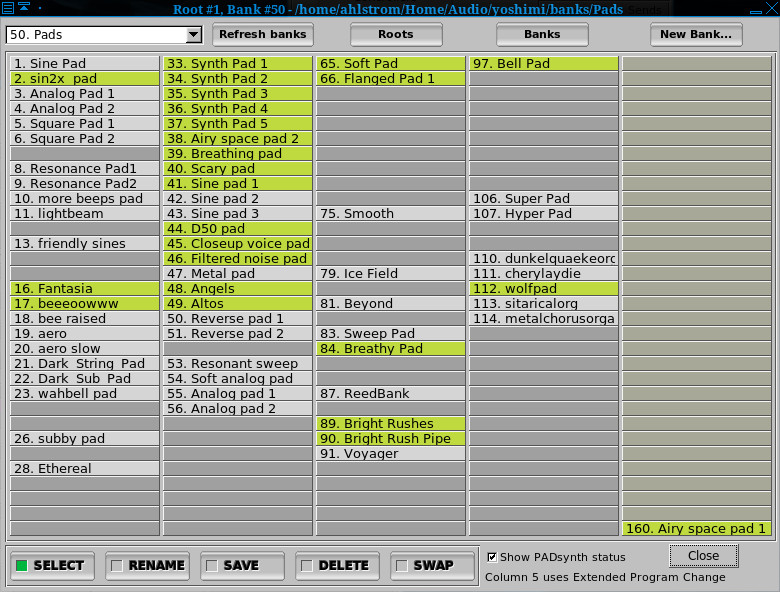
\includegraphics[scale=0.75]{menu/Instrument/show-pads-bank.jpg}
   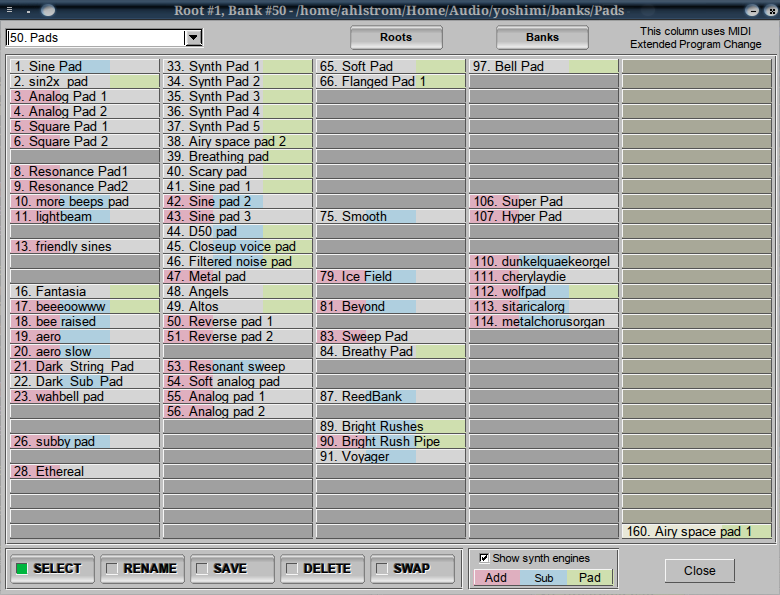
\includegraphics[scale=0.75]{1.3.6/show_pads_bank.png}
   \caption[Show Pads Instruments]{Show Pads Instruments}
   \label{fig:show_pads_bank}
\end{figure}

   Note that many of these Pads instruments also use the Add and Sub
   components as well.

\subsubsection{Menu / Instrument / Show Banks...}
\label{subsubsec:menu_instrument_show_banks}

   This menu entry brings up a dialog that shows all of the banks present in
   the current root.

\begin{figure}[H]
   \centering 
   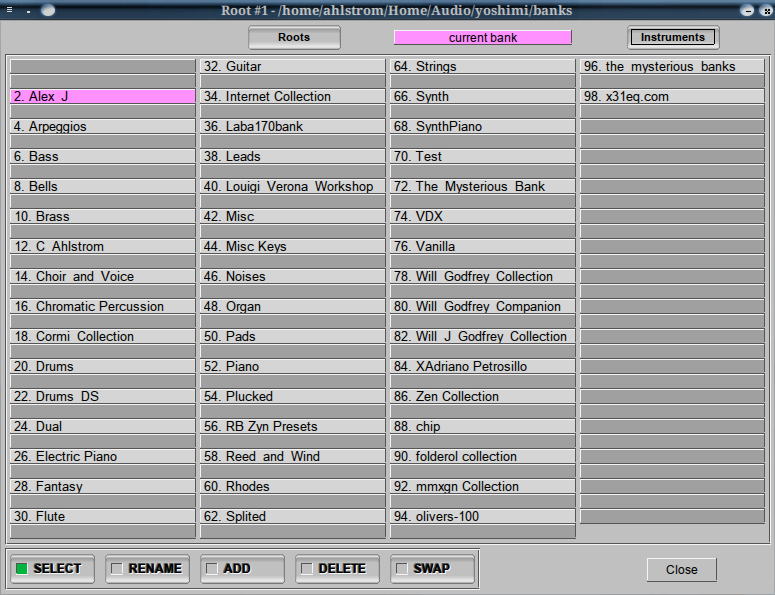
\includegraphics[scale=0.75]{1.3.6/show_CA_banks.png}
   \caption[Show Banks]{Show Banks in Current Root}
   \label{fig:show_ca_banks}
\end{figure}

   This figure illustrates a setup where the installed banks were combined with
   banks downloaded from various web sites.
   The following list shows that the interface elements in the banks dialog
   are slightly different from the instruments dialog.

   \begin{enumber}
      \item \textbf{Roots}
      \item \textbf{Current Bank} (passive display element)
      \item \textbf{Instruments}
      \item \textbf{SELECT}
      \item \textbf{RENAME}
      \item \textbf{ADD}
      \item \textbf{DELETE}
      \item \textbf{SWAP}
      \item \textbf{Close}
   \end{enumber}

   \setcounter{ItemCounter}{0}      % Reset the ItemCounter for this list.

   \itempar{Roots}{banks!roots}
   Banks Roots.
   "Roots" button.
   Shows a list of directories that can serve as "root" directories.

   \itempar{current bank}{banks!current bank}
   \index{current!bank}
   Current Bank.  Simply indicates the current bank via color-highlighting.
   Note that one can left-click on a bank in this dialog to make it the
   current bank.  This setting is saved across \textsl{Yoshimi} restarts.

   \itempar{Instruments}{banks!instruments}
   Banks Instruments.
   \index{current!bank}
   Brings up a banks dialog that shows the instruments in the current bank.

   \itempar{SELECT}{banks!SELECT}
   Banks SELECT.
   When this button is selected, then clicking on a bank makes it the current
   bank.

   (Although we don't show a figure for it, note that some banks provide
   instruments with numbers in the extended program-change range (above
   127) prepended to the file-names.)

   \itempar{RENAME}{banks!RENAME}
   Banks RENAME.
   When this button is selected, then clicking on a bank brings
   up a small dialog to rename the clicked-on bank.
   However, one might also experience the following warning message:

   \begin{verbatim}
      This bank directory cannot be changed
   \end{verbatim}

   \itempar{ADD}{banks!ADD}
   Banks ADD.
   Selecting this button and clicking an empty bank entry brings up a small
   dialog to create a new empty bank name for that entry.
   If one clicks on an existing bank entry, then a small dialog comes up
   stating that the bank number selected is already in use.
   However, one might also experience the following warning message:

   \begin{verbatim}
      This bank directory cannot be changed
   \end{verbatim}

   \itempar{DELETE}{banks!DELETE}
   Banks DELETE.
   Selecting this button and clicking an empty bank entry does nothing.
   Selecting this button and clicking an existing bank entry brings up a
   small dialog asking one if this bank is really to be deleted.
   However, one might also experience the following warning message:

   \begin{verbatim}
      This bank directory cannot be changed
   \end{verbatim}

   \itempar{SWAP}{banks!SWAP}
   Banks SWAP.
   Selecting this button, then selecting one bank, and then another,
   swaps the numbering and postion of the selected banks.
   This button is good for minor reorganization of the bank numbers.

\subsubsection{Menu / Instrument / Show Root Paths...}
\label{subsubsec:menu_instrument_show_root_paths}

\begin{figure}[H]
   \centering 
   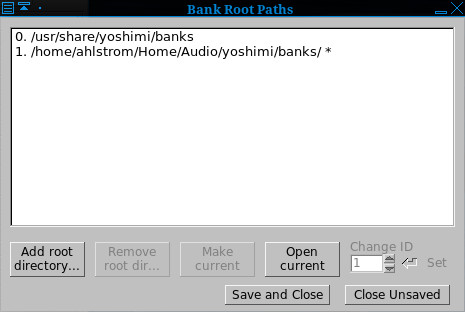
\includegraphics[scale=0.75]{menu/Instrument/show-banks-roots.jpg}
   \caption[Show Root Paths]{Show Root Paths}
   \label{fig:show_banks_roots}
\end{figure}

   \setcounter{ItemCounter}{0}      % Reset the ItemCounter for this list.

   \itempar{Add root directory...}{Root Paths!add directory}
   Show Root Paths Add Root Directory.
   To add a bank root path:

   \textsl{Yoshimi} (as installed by Debian Linux) provides a default bank at
   \texttt{/usr/share/yoshimi/banks}.
   To add one's own directory, navigate to "Yoshimi / Instrument / Show Root
   Paths ...".  Then click on "Add root directory...".

   Once selected, one will see that \texttt{/usr/share/yoshimi/banks}
   is marked with an asterisk.  One can select the new root directory,
   and make it current by clicking the "Make current" button.
   Then the Banks dialog will show all the banks in that directory, one bank
   per subdirectory (each subdirectory "is" a bank).

\begin{figure}[H]
   \centering 
   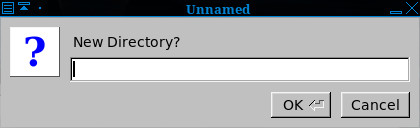
\includegraphics[scale=0.75]{menu/Instrument/new-directory.jpg}
   \caption{Add Root Directory}
   \label{fig:add_root_directory}
\end{figure}

   \itempar{Remove root directory...}{Root Paths!remove directory}
   Show Root Paths Remove Root Directory.
   If a path is selected, then this button is active, and can be used to
   delete the selected path from the "root paths" list.

   \itempar{Make current}{Root Paths!make current}
   Show Root Paths Make Current.
   \index{current!root}
   This button marks the currently-selected path as the "current root" path.

   \itempar{Open current}{Root Paths!open current}
   Show Root Paths Open Current.
   This button opens the current root path.

   \itempar{Change ID}{Root Paths!change ID}
   Show Root Paths Change ID.

   Values: \texttt{0* to 127}

   \textsl{
   We need to know more about how this ID can be used.
   Is it a way to make the path selectable via an extended MIDI control, or
   some other automation method?
   }

%-------------------------------------------------------------------------------
% vim: ts=3 sw=3 et ft=tex
%-------------------------------------------------------------------------------


%-------------------------------------------------------------------------------
% yum_menu_instruments
%-------------------------------------------------------------------------------
%
% \file        yum_menu_instruments.tex
% \library     Documents
% \author      Chris Ahlstrom
% \date        2016-02-27
% \update      2018-12-29
% \version     $Revision$
% \license     $XPC_GPL_LICENSE$
%
%     Provides the Menu / Instruments section of the manual.
%
%-------------------------------------------------------------------------------

\subsection{Menu / Instruments}
\label{subsec:menu_instrument}

   The \textsl{Yoshimi} Instruments menu lets one select instruments and work
   with banks of instruments.

   While the \textbf{Instrument Menu} allows for the management of parts, the
   \textbf{Part Edit} dialog, described in
   \sectionref{subsec:bottom_panel_instrument_edit},
   is where one would start for the the creation of a new part/instrument.

   When opening an instrument bank one can now tell exactly which synth engines
   are used by each instrument. This is represented by three pale background
   colours:

   \begin{itemize}
      \item \textbf{\textcolor{red}{Red}}: ADDsynth
      \item \textbf{\textcolor{blue}{Blue}}: SUBsynth
      \item \textbf{\textcolor{green}{Green}}: PADsynth
   \end{itemize}

   These new coloured engine backgrounds aren't just pretty. They give real
   information about expected processor load, and time taken to be ready when
   loaded:

   \begin{itemize}
      \item Processor Load, low to high:
         \textbf{\textcolor{green}{PAD}},
         \textbf{\textcolor{blue}{SUB}}, then
         \textbf{\textcolor{red}{ADD}}.
      \item Time to initialise, low to high:
         \textbf{\textcolor{blue}{SUB}},
         \textbf{\textcolor{red}{ADD}},
         \textbf{\textcolor{green}{PAD}}.
   \end{itemize}

   If the instruments are kits they are scanned to find out if
   \textsl{any} member of the kit contains each engine.
   This scanning is duplicated in the current part, the mixer panel for the
   currently loaded instruments, and in the Instrument Edit window the same
   colours highlight the engine names when they are enabled with the check
   boxes.

   The following sub-menus are provided, as shown in
   \figureref{fig:yoshimi_instrument_menu}.

\begin{figure}[H]
   \centering
   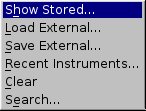
\includegraphics[scale=0.9]{1.6.0/menu_instrument.png}
   \caption{Yoshimi Menu, Instruments}
   \label{fig:yoshimi_instrument_menu}
\end{figure}

   This new version of the \textbf{Instruments}
   menu is somewhat different than
   the old version.  It is actually simpler and easier to use, while still
   offering all of the power of the setting up of instruments in
   \textsl{Yoshimi}.

   \begin{enumber}
      \item \textbf{Show Stored...}
      \item \textbf{Load External...}
      \item \textbf{Save External...}
      \item \textbf{Recent Instruments...}
      \item \textbf{Clear}
      \item \textbf{Search}
   \end{enumber}

%  \setcounter{ItemCounter}{0}      % Reset the ItemCounter for this list.

\subsubsection{Menu / Instrument / Show Stored...}
\label{subsubsec:menu_instrument_show}

   Instruments are stored in banks
   (see \sectionref{subsec:concepts_banks_and_roots}).
   The banks (and current bank setting) are
   loaded/saved automatically by the program, so one doesn't have to worry
   about saving the banks before the program exits. On program start, the last
   used bank is loaded. A single bank can store up to 128 instruments.
   However, there is space for a number of additional instruments in the bank,
   the extended-program section, to allow up to 160 instruments in a bank.

   When the \textbf{Show Stored...} button is selected, a dialog comes
   up that shows all of the instruments present in the currently-selected
   bank.

\begin{figure}[H]
   \centering
   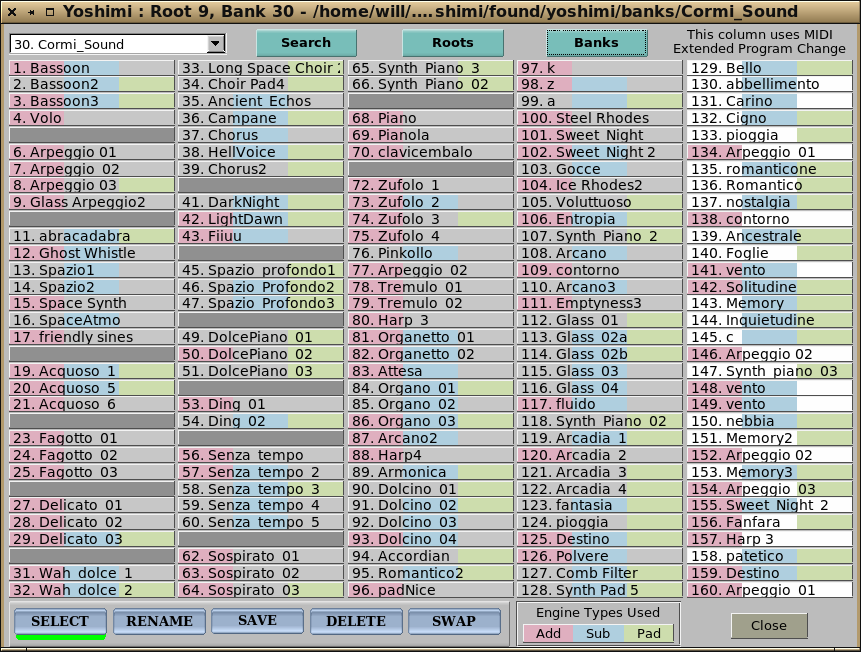
\includegraphics[scale=0.75]{2.3.0/instruments.png}
   \caption[Show Stored Instruments]{Instruments Stored in Current Banks}
   \label{fig:instruments_show_stored}
\end{figure}

   As \figureref{fig:instruments_show_stored},
   shows, this is a very complex dialog with a lot of options.
   The figure shows a default setup, with the bank of instruments at location
   30, \textbf{30. Misc}, listed.
   If one drops this list down (shown later), one also observes that the banks
   are numbered in increments of 5, to make it easier for a user to insert his
   or her own bank(s) of instruments. The default set of banks are spaced 5
   apart for this reason. If we add more than 25 banks in future versions of
   \textsl{Yoshimi}, then a \textsl{clean} install will wrap round starting with
   location 2 and again spaced 5 apart, and so-on until all spaces are filled.
   For an existing setup, new entries will just be slotted in where they
   will fit.

   Also, if one deletes banks or instruments by some external means, the next
   time \textsl{Yoshimi} starts, it will notice their absence and quietly
   remove their entries.

   Note how \textsl{Yoshimi} shows the colour coding for the
   synth-sections used in each instrument:
   red for ADDsynth, blue for SUBsynth, and green for PADsynth.
   This used to be switchable as not fetching the colour information from the
   banks meant startup was sometimes slightly faster. However this then
   interfered with later developments that use this information for other
   purposes so it has now been removed.

   Also note how the numbers at the beginning of the filenames are used as
   an "instrument" or "program" number.  These numbers can be used in MIDI
   Program Change commands.

\index{new!Instrument Highlight}
   A new feature since \textsl{Yoshimi} V 1.7.2 is highlighting the last
   instrument seen. In this case, the third one in the list. This is
   particularly useful for banks where the internal name is different from the
   filename.

   All of the instrument files (such as \texttt{0001-Arpeggio1.xiz})
   with filenames starting with numbers (no matter how many digits)
   will be shown in the corresponding slot number.
   Variations in filename after the number are ignored; the files
   are treated as the same instrument.

   Those instrument files
   without numbers (or larger numbers?) will start
   with numbers at 129 or above ("Extended Program Change") up to 160.
   One could give them numbers by renaming them outside of \textsl{Yoshimi},
   then reloading the bank.
   One can also fix unnumbered ones simply by loading them, then re-saving them
   to the same slot. It's then probably best to swap them into the main set,
   if there is space.

   \index{extended program}
   Note that MIDI CC
   (see \sectionref{paragraph:menu_yoshimi_settings_ccs})
   can be set to access voices from 129 to 160.
   All the Bank controls in the \textbf{MIDI} settings tab take immediate
   effect when set.
   Bank and program changes can be completely disabled in the settings tab;
   some hardware synths don't play nice with it.

   Learning how to use the Instruments dialog is an important way to make
   instruments easier to manage, and so this will be a long discussion.

%  An important pair of concepts in \textsl{Yoshimi} are
%  \textsl{banks} and \textsl{roots}.  These concepts are described in
%  \sectionref{subsec:concepts_banks_and_roots}.

   Here is a list of the user-interface items in the instruments/banks dialog:

   \begin{enumber}
      \item \textbf{Bank Names}
      \item \textbf{Search}
      \item \textbf{Roots}
      \item \textbf{Banks}
      \item \textbf{Instrument and Bank Matrix}
      \item \textbf{SELECT}
      \item \textbf{RENAME}
      \item \textbf{SAVE}
      \item \textbf{DELETE}
      \item \textbf{SWAP}
%      \item \textbf{Show synth engines}
      \item \textbf{Close}
   \end{enumber}

   \setcounter{ItemCounter}{0}      % Reset the ItemCounter for this list.

   \itempar{Bank Names}{instruments!bank names}
   Instruments Bank Name.
   This item is a drop-down list of the available instrument banks in the
   currently-selected \textbf{root} directory.
   Basically, each bank is a directory name, with a number prepended.
   The banks are found under the current root, which is a also a directory
   name, and is the name of the parent directory of a set of banks.
   Here is the Bank Names drop-down list for the default setup, which has the
   default banks provided by the basic \textsl{Yoshimi} installation.

\begin{figure}[H]
   \centering
%  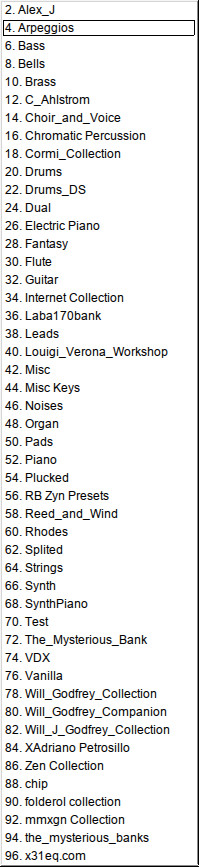
\includegraphics[scale=0.75]{menu/Instrument/bank-list.jpg}
   \includegraphics[scale=0.75]{2.3.0/banks.png}
   \caption[A Sample Bank List]{A Sample Bank List}
   \label{fig:bank_list}
\end{figure}

   And here is the directory listing associated with it, in the order
   produced by the UNIX/Linux \texttt{ls -1}
   (list single-column) command (shown in
   two columns to save space):

   \begin{verbatim}
      Arpeggios          Plucked
      Bass               Reed_and_Wind
      Brass              Rhodes
      Choir_and_Voice    Splited
      Drums              Strings
      Dual               Synth
      Fantasy            SynthPiano
      Guitar             The_Mysterious_Bank
      Misc               Will_Godfrey_Collection
      Noises             Will_Godfrey_Companion
      Organ              chip
      Pads               Cormi_Sound
   \end{verbatim}

   The directories (banks) shown above come from the default \textbf{root}
   when \textsl{Yoshimi} and its data files are installed:

   \begin{verbatim}
      /usr/share/yoshimi/banks
   \end{verbatim}

   If one installed \textsl{Yoshimi} by building the source code, then
   this directory is:

   \begin{verbatim}
      /usr/local/share/yoshimi/banks
   \end{verbatim}

   Note that the directory that holds the banks is shown in the title bar.
   Another good source of banks, if one installs \textsl{ZynAddSubFX}, is:

   \begin{verbatim}
      /usr/share/zynaddsubfx/banks
   \end{verbatim}

   Note that there are only 128 \textsl{Yoshimi} banks
   supported in a \textsl{Yoshimi} root.
   If the list of banks takes up about half of the available slots, it might be
   time to move some of those banks to a new root directory.

   The numbers in the drop-down list are generated by \textsl{Yoshimi} the
   first time it sees a new root path or a new bank within the root path.
   Once set, these numbers will never change unless one actually moves them
   around (using the \textbf{SWAP} button).

   The bank number is also the MIDI ID for the bank;
   one can be sure that it will always
   be there for bank changes, no matter how many banks are added later.
   \textsl{Yoshimi} always lists the banks in ID order, not alphabetical
   order, so one can group them sensibly and permanently.
   However, at first-time creation \textsl{Yoshimi} sets the IDs in
   alphabetical order and tries to space them evenly over the range to
   provide some wiggle room.
   Selecting one of the items in this drop-down list selects the bank and
   loads it into the Banks dialog.

   \index{anti-auto-clutter}
   Right-clicking or left-clicking on a bank in the drop-down list
   causes the instrument list of the previous bank to be replaced by the
   instrument list of the newly-selected bank.

   \index{new!instruments search}
   \itempar{Search}{instruments!search}
   Instruments Search Button.
   This feature arrived with \textsl{Yoshimi} V 1.6.0 and provides a
   way of finding instruments of a given type right across all known banks and
   bank roots.


\begin{figure}[H]
   \centering
%  \includegraphics[scale=0.75]{menu/Instrument/bank-list.jpg}
   \includegraphics[scale=0.5]{2.3.0/search.png}
   \caption[A search list List]{A search list}
   \label{fig:bank_search}
\end{figure}
   The top field is a drop-down menu that gives all the types
   \textsl{Yoshimi} recognises, and below this is the list of those
   most recently found. As well as the names of the instruments
   one sees the bank root ID, bank ID and instrument number. All of these
   are the values that will be recognised by MIDI.

   Clicking on any entry will immediately load the instrument into the
   current part \textbf{without} changing the settings for current bank or
   root.

   \itempar{Roots}{instruments!roots}
   Instruments Roots Button.
   Shows a list of directories that can serve as "root" directories.
   The "Bank Root Paths" dialog discussed in
   \sectionref{subsubsec:menu_patch_sets_patch_bank_roots}\hspace{4pt}in
   \figureref{fig:show_patch_banks}\hspace{4pt}shows
   the system root (e.g. \texttt{/usr/share/yoshimi/banks}) and
   a user's home location for his/her banks and roots.

   \itempar{Banks}{instruments!banks}
   Banks Button.
   This item brings up a Banks dialog showing all of the banks present in the
   current root.
   It is an alternative to using the \textbf{Bank Names} drop-down list to
   select a bank.  It is also a way to reorganise and renumber the
   banks without using the Linux console or a file-explorer application to do
   so.

   \itempar{Instrument and Bank Matrix}{instruments!bank matrix}
   Instruments Bank Matrix.
   Shows the instruments that are in the currently selected bank.

   The next few items are selector buttons that determine what happens when one
   clicks on an instrument name.

   \itempar{SELECT}{instruments!SELECT}
   Instruments SELECT.
   When this button is selected, then clicking on an instrument selects that
   instrument as the instrument for the current Part active in the main
   window.  In the main window of \textsl{Yoshimi}, that instrument name will
   appear in the currently-selected \textbf{Part}.  If \textsl{Yoshimi} is
   writing to a console window then each part, when clicked, will be shown:

   \begin{verbatim}
		yoshimi> Loaded 64 "Hyper Organ1" to Part 1
		Loaded 65 "Hyper Arpeggio" to Part 1
		Loaded 10 "Arpeggio11" to Part 1
		Loaded 41 "Soft Arpeggio4" to Part 1
		Loaded 67 "Glass Arpeggio1" to Part 1
   \end{verbatim}

   \itempar{RENAME}{instruments!RENAME}
   Instruments RENAME.
   When this button is selected, then clicking on a bank brings
   up a small dialog to rename the clicked-on bank.
   However, one will see the following warning message if trying to rename a
   file that is in a directory not modifiable by normal users:

   \begin{verbatim}
      ! Could not rename instrument 39 to Soft Arpeggio5 [Close]
   \end{verbatim}

   Note that, as soon as this operation is done, the auto-selector (green
   check-box) moves back to the \textbf{SELECT} button.

   \itempar{SAVE}{instruments!SAVE}
   Instruments SAVE.
   When this button is selected, then clicking on a bank saves
   the instruments as currently configured.
   A prompt like the following will appear:

   \begin{verbatim}
      ? Overwrite the slot no. 43 ?  [No/Yes]
   \end{verbatim}

   However, if one answers yes, and the instrument is in a non-modifiable
   directory, then one will see the following error message:

   \begin{verbatim}
      ! Could not save to this location [Close]
   \end{verbatim}

   \itempar{DELETE}{instruments!DELETE}
   Instruments DELETE.
   Selecting this button and clicking an empty bank entry does nothing.
   Selecting this button and clicking an existing bank entry brings up a
   small dialog asking one if this bank is really to be deleted.

   \begin{verbatim}
      ? Clear the slot no. 68?  [No/Yes]
   \end{verbatim}

   However, if one answers yes, and the instrument is in a non-modifiable
   directory, then one will see the following error message:

   \begin{verbatim}
      ! Could not clear this location  [Close]
   \end{verbatim}

   \itempar{SWAP}{instruments!SWAP}
   Instruments SWAP.
   Selecting this button, then selecting one instrument, and then another,
   swaps the numbering and position of the selected instruments.
   However, one might also experience the following warning message:

   \begin{verbatim}
      ! Could not swap these locations  [Close]
   \end{verbatim}

   Note that all of the above error messages are also shown in the console, if
   it is where \textsl{Yoshimi} is running.  For example:

   \begin{verbatim}
      40 Failed to remove /usr/local/share/yoshimi/banks/Arpeggios/0041-Soft
      Arpeggio3.xiz Permission denied
   \end{verbatim}

%   \itempar{Show synth engines}{instruments!show engines}
%   If enabled, then the usage of each of the \textsl{Yoshimi} synthesis
%   engines is indicated by color coding, as shown in the figure above.

%   \textbf{Note} This also affects the new search feature, as at startup there
%    is a scan of all banks checking for the instrument engines and type.

   \itempar{Close}{instruments!Close}
   Closes the window.

%  Here is a more conventional view of instruments, supplied with
%  \textsl{Yoshimi}, shown in
%  \figureref{fig:show_pads_bank}.
%
% \begin{figure}[H]
%    \centering
% %  \includegraphics[scale=0.75]{menu/Instrument/show-pads-bank.jpg}
%    \includegraphics[scale=0.75]{1.3.6/show_pads_bank.png}
%    \caption[Show Pads Instruments]{Show Pads Instruments}
%    \label{fig:show_pads_bank}
% \end{figure}
%
%    Note that many of these Pads instruments also use the Add and Sub
%    components as well.

\subsubsection{Menu / Instrument / Load External...}
\label{subsubsec:menu_instrument_load}

   This menu entry simply brings up a file dialog, allowing the user to
   navigate to an arbitrary directory, and then to a solitary instrument file
   (\texttt{*.xiz}), and load it into the current Part.

\begin{figure}[H]
   \centering
   \includegraphics[scale=0.5]{2.3.0/filer.png}
   \caption{Instruments, Load External}
   \label{fig:instruments_load_external}
\end{figure}

   These "xiz" files are normally found in a \texttt{banks} directory, but
   this operation allows access to instruments that are not located in a bank.

   \begin{itemize}
      \item If loading an external instrument file with no internal name,
         the file leafname will be shown.
      \item If loading an external instrument file with the name
         \textsl{Simple Sound}, the name \textsl{No Title} will be given.
      \item If loading a patch set that has unnamed instruments, or ones with
         the name \textsl{Simple Sound}, those will be given the name \textsl{No
         Title}.
   \end{itemize}

   This dialog has a number of user-interface elements to discuss:

   For further details see \sectionref{subsec:interface_filer}.

\iffalse
   \begin{enumber}
      \item \textbf{Show}
      \item \textbf{Favorites}
      \item \textbf{Create a new directory}
      \item \textbf{Instrument List}
      \item \textbf{XML Preview}
      \item \textbf{Preview}
      \item \textbf{Show hidden files}
      \item \textbf{Directory Bar}
      \item \textbf{Filename}
      \item \textbf{OK}
      \item \textbf{Cancel}
   \end{enumber}

   These elements are used in a number of different places in
   \textsl{Yoshimi}.
   Therefore, we will explain them all once, here.

   \setcounter{ItemCounter}{0}      % Reset the ItemCounter for this list.

   \itempar{Show}{Load External!show}
   Show types of files.
   This item shows a file filter for selecting instrument files.
   The types of filters are as follows (screen shot not available):

   \begin{enumber}
      \item \textbf{(\{*.xiz\})} (compressed XML files)
      \item \textbf{All Files (*)}
      \item \textbf{Custom Filter}
   \end{enumber}

   \itempar{Favorites}{Load External!favorites}
   Favourite directories.
   Provides a list of options and favourite directories in which to find
   instrument files.

\begin{figure}[H]
   \centering
   \includegraphics[scale=0.75]{menu/Instrument/favorites-dropdown.jpg}
   \caption{Manage Favorites Drop-Down List}
   \label{fig:open_instrument_favorites}
\end{figure}

   \begin{enumber}
      \item \textbf{Add to Favorites}
      \item \textbf{Manage Favorites}
      \item \textbf{File Systems}
      \item \textbf{\textsl{(current favourite directories)}}
   \end{enumber}

   \index{Add to Favorites}
   \textbf{Add to Favorites}
   simply adds the currently selected directory shown in the instrument list
   to the list of favourites.

   To add favourites in the file dialog, navigate to the desired directory.
   Then click \textbf{Favorites}, and select \textbf{Add to Favorites}.

   Once one has a number of favourites set up,
   there is a \textbf{Manage Favorites} that can be used.
   For example, if one needs to get rid of a directory, one can use the
   \textbf{Manage Favorites}
   \index{Manage Favorites}
   dialog, shown in
   \figureref{fig:manage_instrument_favorites} below,
   to do that.

\begin{figure}[H]
   \centering
   \includegraphics[scale=0.75]{menu/Instrument/manage-favorites.png}
   \caption{Manage Favorites Dialog}
   \label{fig:manage_instrument_favorites}
\end{figure}

   \textbf{File Systems} \index{File Systems}
   Provides a list of all file systems starting at root ("\texttt{/}").
   This list can be pretty confusing, with a lot of entries.
   But note that one navigates to ("\texttt{/}"), and from there to
   \texttt{/usr/share/yoshimi/banks} to get easy access to all the
   instruments that are preinstalled with
   \textsl{Yoshimi}.
   Generally, one will want to use only
   \textbf{Add to Favorites} and \textbf{Manage Favorites}.

   \itempar{Create Directory}{Load External!create new directory}
   Creates a New Directory.
   This little symbol brings up a small "New Directory?" dialog (not shown
   here, it is very simple and stock) into which one can type a directory
   name to be added to the current directory of the instrument list.

   \itempar{Instrument List}{Load External!instrument list}
   Provides a list of the instrument files available in the current
   directory.  Also shown are sub-directories (if available)
   that might contain more instruments, and a ("\texttt{../}") entry
   to navigate to the parent directory.

   \itempar{Preview}{Load External!preview checkbox}
   If one thinks the preview feature is not useful, uncheck this check-box.
   so that one doesn't see the preview window.  As a bonus, one can see more
   of a long instrument file-name.

   \itempar{Preview pane}{Load External!preview pane}
   XML Preview.
   This box can show the beginning of the XML data of an instrument file.
   \textbf{Bug:}
   \index{bugs!compressed XML preview}
   The XML preview feature shows the XML only if the XML is not compressed.

   \itempar{Show hidden files}{Load External!show hidden files}
   Shows file that are hidden.  Not sure how useful this feature is;
   who would hide a \textsl{Yoshimi} instrument file?

   \itempar{Directory Bar}{Load External!directory bar}
   Provides an alternate way to move up through the directory structure.
   Click on each of the small bevelled rectangles to move around in the
   directory hierarchy.

   \itempar{Filename}{Load External!filename}
   File Name.
   Provides the full path specification for the instrument file.

   \itempar{OK/Cancel}{Load External!ok/cancel}
   We don't really need to discuss the \textbf{OK} and \textbf{Cancel}
   buttons, do we?  OK, we'll cancel that discussion.
\fi
\subsubsection{Menu / Instrument / Save External...}
\label{subsubsec:menu_instrument_save}

   This menu entry simply brings up a file dialog, allowing the user to
   navigate to an arbitrary directory, and then save the current Part
   to a solitary instrument file (\texttt{*.xiz}).

\begin{figure}[H]
   \centering
   \includegraphics[scale=0.75]{2.3.0/save_ext_instrument.png}
   \caption{Instruments, Save External}
   \label{fig:instruments_save_external}
\end{figure}

   This dialog is very similar to the \textbf{Load External} dialog.
%   Note the large question mark in the XML preview, indicating a compressed XML
%   file.  If uncompressed, then an XML text preview will be shown.

   The instrument save action saves only what is essential to the instrument,
   and not the part it may be sitting in.  If there have been no changes in the
   instrument, then a \textbf{Nothing to save!} dialog appears.

   From \textsl{Yoshimi} V1.7.4 there is a warning if the 'type' filed has
   not been filled in. One can ignore this and save regardless, but it is
   hoped the gentle reminder will encourage more people to fill it in.

\subsubsection{Menu / Instrument / Recent Instruments...}
\label{subsubsec:menu_instrument_recent}

   This menu brings up a simple window with a list of the most recent
   instruments that have been selected.  A single-click on the desired
   instrument will load it.

\subsubsection{Menu / Instrument / Clear}
\label{subsubsec:menu_instrument_clear}

   Normally this menu entry simply clears the instrument that is loaded into
   the current Part.  This converts the instrument to a
   \textsl{Simple Sound} patch.
   However, if the Ctrl key is held down when clicking on the entry, the entire
   part will be returned to default values, including Controllers etc.

   In either case, the menu entry brings up a prompt with details of exactly what
   will be cleared.

\begin{figure}[H]
   \centering
   \includegraphics[scale=0.75]{2.3.0/clear_instrument.png}
   \caption{Clear Instrument Dialog}
   \label{fig:clear_instrument_dialog}
\end{figure}
\begin{figure}[H]
   \centering
   \includegraphics[scale=0.75]{2.3.0/clear_part.png}
   \caption{Clear Part Dialog}
   \label{fig:clear_part_dialog}
\end{figure}

   \textbf{No} is the default action.

\subsubsection{Menu / Instrument / Search}
\label{subsubsec:menu_instrument_search}

   This entry provides a quicker route to the instrument search feature described
   in \sectionref{subsubsec:menu_instrument_show}
\subsubsection{Menu / Instrument / Misc Notes}
\label{subsubsec:menu_instrument_misc_notes}

   There are still many instruments out there with
   no internal title. This fact applies to both external files and instruments
   in banks, and means that, once loaded, one does not know what instruments
   one has. So now, if the internal name is missing, \textsl{Yoshimi} will use
   the leaf-name of the file.  When one saves an instrument to a bank slot, it
   will get a filename with the internal name as the leaf-name.  When saving
   an instrument to an external file, the first offered will be the internal
   name and in the current directory, but this can be changed if desired.

   The part and mixer name fields will always show the (possibly adjusted)
   internal name regardless of the external filename, which could easily have
   been changed at some time.  The instrument banks will always show the file's
   leaf-name, so it more-or-less matches external files (what one sees from a
   file display).  As soon as one edits an instrument, if it was \textsl{Simple
   Sound}, the name will be changed to \textsl{No Title}.  \textsl{Yoshimi}
   generally won't let one rename an instrument to \textsl{Simple Sound}.

   Default instruments are never saved, not even in patch sets and states, but
   if the parts are activated, that fact \textsl{is} saved; it's a part
   feature, not an instrument one.

   Patch sets will save all other instruments regardless of whether they are
   activated or not.

   While testing all these features, Will created a new multi-part instrument
   kit.  It's now in the \textsl{Companion} set and is called \textsl{Pad Kit}.

%-------------------------------------------------------------------------------
% vim: ts=3 sw=3 et ft=tex
%-------------------------------------------------------------------------------


%-------------------------------------------------------------------------------
% yum_menu_patch_sets
%-------------------------------------------------------------------------------
%
% \file        yum_menu_patch_sets.tex
% \library     Documents
% \author      Chris Ahlstrom
% \date        2016-02-27
% \update      2018-03-11
% \version     $Revision$
% \license     $XPC_GPL_LICENSE$
%
%     Provides the Menu / Instruments section of yoshimi-user-manual.tex,
%     for the 1.3.8 and above versions of Yoshimi.  That menu entry has changed
%     a lot.
%
%-------------------------------------------------------------------------------

\subsection{Menu / Patch Sets}
\label{subsubsec:menu_patch_sets}

   This new menu entry is part of the very nice reorganization and simplification
   of the handling of roots and banks in the new \textsl{Yoshimi}.  The
   \textbf{Patch Sets} menu replaces the old \textbf{Parameters} menu.  Do you
   like the new name?  The patch set saves all of the settings, including effects
   and instruments.  Patch sets will save all other instruments regardless of
   whether they are activated or not.  Default instruments are never saved, not
   even in patch sets, but if the parts are activated that fact \textsl{is}
   saved.  It is a part feature, not an instrument feature.

   \textsl{Yoshimi} stamps its configuration XML files with its own major and
   minor version numbers so it is possible to tell which version created the
   files, or whether they were created by \textsl{ZynAddSubFX}.

   The main dialog is somewhat similar in layout and function to the
   dialog shown in
   \figureref{fig:instruments_show_stored},
   for managing instruments in a selected bank.

\subsubsection{Menu / Patch Sets / Show Patch Banks...}
\label{subsubsec:menu_patch_sets_show_patch_banks}

   The \textbf{Banks} window has had some button shuffling, and one can
   import and export banks as well.

\begin{figure}[H]
   \centering 
%  \includegraphics[scale=0.75]{menu/Instrument/show-banks-roots.jpg}
%  \includegraphics[scale=0.75]{1.3.9/patch_sets_show_patch_banks.png}
   \includegraphics[scale=0.75]{1.5.7/Bank.png}
   \caption[Show Patch Banks]{Show Patch Banks}
   \label{fig:show_patch_banks}
\end{figure}

   Here is a list of the user-interface items in the patch-banks dialog:

   \begin{enumber}
      \item \textbf{Roots}
      \item \textbf{current bank}
      \item \textbf{Instruments}
      \item \textbf{Bank Matrix}
      \item \textbf{SELECT}
      \item \textbf{RENAME}
      \item \textbf{SAVE}
      \item \textbf{DELETE}
      \item \textbf{SWAP}
      \item \textbf{IMPORT}
      \item \textbf{EXPORT}
      \item \textbf{Close}
   \end{enumber}

   \setcounter{ItemCounter}{0}      % Reset the ItemCounter for this list.

   \itempar{Roots}{Roots!root directories}
   Show Patch Banks, Root Directories.
   To add a bank root path, delete a bank root path, or manage bank root path,
   press this button.  The result is somewhat similar to a file dialog,
   and is described in detail in 
   \sectionref{subsubsec:menu_patch_sets_patch_bank_roots}, later in
   this sub-chapter.

   \itempar{current bank}{banks!current bank}
   This item is highlighted in pink, and the bank that is actually the current
   bank is also highlighted in pink.  There is no action associated with this
   user-interface element; it merely indicates the currently-selected bank.

   \itempar{Instrument}{banks!instrument}
   This button brings up an instruments window similar
   to the one shown in
   \figureref{fig:instruments_show_stored}, which shows
   the instruments collected in the currently-selected bank.
   Clicking on a bank in the dialog also brings up the instruments window.

   \itempar{Bank Matrix}{banks!matrix}
   This view shows all of the banks available in the current root.
   Left-clicking on a bank in the dialog brings up the Instruments window for
   that bank.
   Right-clicking on a bank in the dialog brings up the Instruments window for
   that bank, but also closes the banks window, to reduce clutter.

   \itempar{IMPORT}{banks!IMPORT}
   There are a number of benefits to using the IMPORT/EXPORT buttons
   rather than dealing with the directories externally.
   One has far greater control where things go when
   importing, and it's much easier to identify the bank to export.

   When importing or exporting,
   \textsl{Yoshimi} refuses to overwrite exisiting banks or
   directories. That is a flat refusal for exporting, but for importing it will
   add a numeric suffix to the name.

   Importing will copy \textsl{only} in files that
   \textsl{Yoshimi} understands, but will notify
   if there were other unrecognised types in there.
   Exporting just dumps out the entire bank contents.

   There are a number of banks in the wild that contain all sorts of extraneous
   stuff, usually copyright notices; one should use only the instrument
   text fields, provided for exactly that purpose.
   Oh, and one bank Will found had subdirectories with pictures,
   and they weren't small!

   In the main part \textbf{Instrument Edit} window there is a new
   \textbf{Default} button top right.
   See \sectionref{subsec:bottom_panel_instrument_edit}.

   We hope this encourages people
   to fill in the Author and Copyright information.
   To set it up, fill in the text field as normal,
   then, while holding down the Ctrl key, click on the button
   (left or middle mouse click) . This text will now be stored in
   one's
   \textsl{Yoshimi} configurionat directory,
   and whenever one creates a new instrument, just
   click on the \textbf{Default} button, and the saved text will be
   filled in.

   \itempar{EXPORT}{banks!EXPORT}
   Export of banks is described in the previous section.

   The buttons \textbf{SELECT}, \textbf{RENAME}, \textbf{SAVE},
   \textbf{DELETE}, and \textbf{SWAP} behave similarly to the same buttons in
   the Instruments window, as
   described in the discussion at
   \sectionref{subsubsec:menu_instrument_show}.

\subsubsection{Menu / Patch Sets / Load External...}
\label{subsubsec:menu_patch_sets_load}

   This menu entry simply brings up a file dialog, allowing the user to
   navigate to an arbitrary directory, and then to a solitary instrument file
   (\texttt{*.xmz}), and load it into the current set of parts.

\begin{figure}[H]
   \centering 
   \includegraphics[scale=0.75]{menu/Parameters/open-parameters.jpg}
   \caption{Load Patch Set}
   \label{fig:yoshimi_menu_open_parameters}
\end{figure}

   These "xmz" files are normally found in a \texttt{presets} directory, but this
   operation allows access to banks that are not located in a particular root.

   When an "xmz" file is loaded, all of the instruments it contains are
   loaded sequentially into the Parts.  Thus, a number of instruments are loaded
   at once.  So, a patch set is a list of instruments that are related by
   being necessary for a given tune, rather than by being located in a
   particular bank.

%  In patch sets, \textsl{Yoshimi} will save named-but-disabled patches.
%  Currently, \textsl{ZynAddSubFX} does not, so be aware when transferring
%  data between the two synthesizers.

\subsubsection{Menu / Patch Sets / Save External...}
\label{subsubsec:menu_patch_sets_save}

   This menu entry simply brings up a file dialog, allowing the user to
   navigate to an arbitrary directory, and then save the current Part
   to a solitary instrument file (\texttt{*.xiz}).

   In patch sets, \textsl{Yoshimi} will save named-but-disabled patches.
   Currently, \textsl{ZynAddSubFX} does not, so be aware when transferring
   data between the two synthesizers.

\begin{figure}[H]
   \centering 
   \includegraphics[scale=0.75]{menu/Parameters/save-parameters.jpg}
   \caption{Save Patch Set}
   \label{fig:yoshimi_menu_save_parameters}
\end{figure}

   Patch set saves include everything that is not part of the main
   configuration, and so saved patch sets
   includes \textbf{Master Volume} and \textbf{Detune}
   \textbf{Part} destinations, \textbf{Humanise},
   and more.
   If nothing has changed, then the following dialog is shown.

\begin{figure}[H]
   \centering 
   \includegraphics[scale=0.75]{menu/Parameters/nothing-to-save.jpg}
   \caption{Patch Set, Nothing to Save}
   \label{fig:yoshimi_menu_nothing_to_save_parameters}
\end{figure}

\subsubsection{Menu / Patch Sets / Recent Sets}
\label{subsubsec:menu_patch_sets_recent_sets}

   This menu entry brings up a dialog box with a list of the recent patch sets
   that have been loaded.  This item makes it easy to move around one's
   frequently-used banks.

\subsubsection{Menu / Patch Sets / Patch Bank Roots}
\label{subsubsec:menu_patch_sets_patch_bank_roots}

   \textsl{Yoshimi} (as installed by Debian Linux) provides a default bank at
   \texttt{/usr/share/yoshimi/banks}.
   To add one's own directory, click on the \textbf{Roots} button.
   It brings up the following dialog.

\begin{figure}[H]
   \centering 
   \includegraphics[scale=0.75]{1.3.9/patch_sets_bank_root_paths.png}
   \caption{Bank Root Paths}
   \label{fig:bank_root_paths}
\end{figure}

   This dialog has a number of buttons, some of which will be disabled if no
   directory in the list is selected.

   Then click on the "Add root directory..." button.  In the file dialog that
   appear, one can use the \textbf{Create Directory} button to make a new
   directory, if desired:

\begin{figure}[H]
   \centering 
   \includegraphics[scale=0.75]{menu/Instrument/new-directory.jpg}
   \caption{New Root Directory?}
   \label{fig:new_root_directory}
\end{figure}

   Otherwise, once can add an existing directory to the list.

   \setcounter{ItemCounter}{0}      % Reset the ItemCounter for this list.

   \itempar{Add root directory...}{Root Paths!add directory}
   Bank Root Paths, Add Root Directory.

   Once selected, one will see that
   \texttt{/usr/share/yoshimi/banks} or
   \texttt{/usr/local/share/yoshimi/banks}
   is marked with an asterisk.  One can select the new root directory via the
   file dialog that appears, and then make it the current root by clicking the
   \textbf{Make current} button.  Then the Banks dialog will show all the banks
   in that directory, one bank per subdirectory (each subdirectory "is" a
   bank).

   \itempar{Remove root directory...}{Root Paths!remove directory}
   Bank Root Paths, Remove Root Directory.
   If a path is selected, then this button is active, and can be used to
   delete the selected path from the "root paths" list.

   \itempar{Make current}{Root Paths!make current}
   Bank Root Paths, Make Current.
   \index{current!root}
   This button marks the currently-selected path as the "current root" path.

   \itempar{Open current}{Root Paths!open current}
   Bank Root Paths, Open Current.
   This button opens the current root path.
   (Does this work?)

   \itempar{Change ID}{Root Paths!change ID}
   Bank Root Paths, Change ID.
   This ID can be used to make the bank selectable via an extended MIDI
   control.

   Values: \texttt{0* to 127}

%-------------------------------------------------------------------------------
% vim: ts=3 sw=3 et ft=tex
%-------------------------------------------------------------------------------


% Removed.  Basically replaced by the Patch Sets menu.
%
% \subsection{Menu / Parameters}

\subsection{Menu / Paths}
\label{subsec:menu_paths}

   This menu entry provides a more direct way to set up the Bank Root and
   the Presets directories.  It contains the following items:

   \begin{enumber}
      \item \textbf{Bank Root Dirs...}
      \item \textbf{Preset Dirs...}
   \end{enumber}

   \paragraph{Bank Root Dirs...}
   The Paths Bank Root Dirs dialog is described in
   \sectionref{subsubsec:menu_patch_sets_patch_bank_roots},
   which shows
   \figureref{fig:bank_root_paths}, and describes this dialog in full.

   \paragraph{Preset Dirs...}
   The \textsl{Yoshimi} preset directories are the locations where
   presets can be found.  When first installed, the system
   preset directory is one of the following, depending on whether
   \textsl{Yoshimi} was installed via a package manager or via source code:

   \begin{verbatim}
      /usr/share/yoshimi/presets
      /usr/local/share/yoshimi/presets
   \end{verbatim}
   
   The user can provide additional directories for the presets, up to a limit
   of 128 directories (the same limit as for roots and banks).
   These directories are useful for containing copies of the system
   presets that one can modify safely, and for providing custom
   presets designed by the user.

   The following items are provided by the preset directory settings:

   \begin{enumber}
      \item \textbf{Preset list}
      \item \textbf{Add preset directory...}
      \item \textbf{Remove preset directory...}
      \item \textbf{Make default}
      \item \textbf{Save and Close}
      \item \textbf{Close Unsaved}
   \end{enumber}

\begin{figure}[H]
   \centering 
   \includegraphics[scale=0.75]{menu/Yoshimi/yoshimi-settings-presets-dirs.jpg}
   \caption[Preset Dirs Tab]{Yoshimi Preset Dirs Dialog}
   \label{fig:yoshimi_presets_dirs_tab}
\end{figure}

   \setcounter{ItemCounter}{0}      % Reset the ItemCounter for this list.

   \itempar{Preset list}{Yoshimi Presets!Preset List}
   This interface element contains a list of preset directories.
   By default, the only directory present is the installed preset directory.
   For example, \texttt{/usr/share/yoshimi/presets}.
   
   \textbf{Tip:}
   \index{tip!preset directory}
   If there is no directory in this dialog, then one must
   add one, otherwise there is no place to store the presets.
   So make this one of the first items specified when first running
   \textsl{Yoshimi}!

   Another example would be this project; let YOSHIMI-DOC be the directory
   where this project is stored.  Then one can add
   \texttt{YOSHIMI-DOC/config/yoshimi/presets} to this list, using the
   button described next.

   \itempar{Add preset directory...}{Yoshimi Presets!Add Directory}
   Use this button and dialog to add a preset directory to the list, for
   easy access.

   Press the \textbf{Add preset directory...} button, revealing the
   following dialog.

\begin{figure}[H]
   \centering 
   \includegraphics[scale=0.75]{menu/Yoshimi/presets-add-a-preset-directory.jpg}
   \caption[Add Preset Directory]{Add a Preset Directory}
   \label{fig:presets_add_a_preset_directory}
\end{figure}

   Navigate to the desired directory, select it, and press the \textbf{Ok}
   button.  (There is no need to press the \textbf{Save and Close} button;
   the directory is added as soon as \textsl{OK} is clicked.  However, one
   tends to want to click it anyway, to be sure.)
   \textsl{Important}:  Restart \textsl{Yoshimi} to use the preset directory.

   \itempar{Remove preset directory...}{Yoshimi Presets!Remove Directory}
   Select one of the preset directories in the preset list, then press this
   button to remove the preset directory from the list of preset
   directories.  It is removed immediately, with no need to confirm the
   deletion, click an OK button, or click a Save button.

   \itempar{Make default presets}{Yoshimi Presets!Make Default}
   Make Default Presets Directory.
   Select one of the preset directories in the preset list, then press this
   button to make the preset directory the default preset directory.
   It should be a directory for which one has write permissions.
   By default, it is \texttt{\textasciitilde/.config/yoshimi/presets}.

\subsection{Menu / Scales}
\label{subsec:menu_scales}

   \textsl{Yoshimi} is a microtonal synthesizer, and is capable of a wide
   range of microtonal scales.

   At present, we're not too experienced with this feature.

\begin{figure}[H]
   \centering 
   \includegraphics[scale=0.9]{menu/yoshimi-menu-scales.jpg}
   \caption{Yoshimi Menu, Scales}
   \label{fig:yoshimi_menu_scales}
\end{figure}

   \begin{enumber}
      \item \textbf{Show Settings...}
      \item \textbf{Load...}
      \item \textbf{Save...}
      \item \textbf{Recent Scales...}
      \item \textbf{Clear}
   \end{enumber}

\subsubsection{Menu / Scales / Show Settings}
\label{subsec:menu_scales_show}

\begin{figure}[H]
   \centering 
   \includegraphics[scale=0.75]{menu/Scales/scale-settings-microtonal.jpg}
   \caption{Yoshimi Menu, Scales Settings}
   \label{fig:yoshimi_menu_scales_settings}
\end{figure}

\paragraph{Scales Basic Settings}
\label{paragraph:menu_scales_basic_settings}

   This item controls the micro-tonal capabilities of \textsl{Yoshimi} and
   some other settings related to tuning. 
   The last entry in the tunings list represents one octave.
   All other notes are deduced from these settings.

   \setcounter{ItemCounter}{0}      % Reset the ItemCounter for this list.

   \itempar{Microtonal}{Enable Microtonal}
   Enable Microtonal Scales.
   When disabled, the synthesizer will use equal-temperament, 12 notes per
   octave.  Otherwise, one can input any scale one desires.

   Values: \texttt{Off*, On}

   \itempar{"A" Freq}{"A"}
   Frequency of the "A" Note.
   Sets the frequency of the "A" key. The standard is 440.0 Hz.

   Values: \texttt{440*}

   \itempar{"A" Note}{"A" MIDI}
   Sets the MIDI Value of the "A" Note.

   Values: \texttt{0 to 127, 69*}

   \itempar{Invert Keys}{keys}
   Allows the keys to be inverted, so that higher-valued keys play lower
   notes.

   Values: \texttt{Off*, On}

   \itempar{Center}{center}
   Center for Inverted Keys.
   This is the center where the notes frequencies are turned upside-down if
   \textbf{Invert keys} is enabled.
   If the center is 60, the note 59 will become 61, 58 will become 62, 61
   will become 59, and so on.

   Values: \texttt{0 to 127, 60*}

   \itempar{Name}{mapping}
   Name of the Mapping.
   For example, the default mapping is called "12tET".

   \itempar{Shift}{key shift}
   Key Shift.
   Shift the scale. If the scale is tuned to A, one can easily tune it to
   another key.

   Values: \texttt{-63 to 64, 0*}

   \itempar{Comment}{comment}
   Comment for Key Mapping.
   Provides a comment or a description of the scale.
   By default, this is "Equal Temperament 12 notes per octave".

   \itempar{Tunings}{tuning}
   Tunings.
   Here one can input a scale by entering all the tunings for one octave. 
   One can enter the tunings in two ways: 

   \begin{enumber}
      \item As the number of cents (1200 cents=1 octave) as a float number
         like "100.0", "123.234"
      \item As a proportion like "2/1" which represents one octave, "3/2" a
         perfect fifth, "5734/6561".  "2/1" is equal to "1200.0" cents.
   \end{enumber}

   The default is a series of values:
   \texttt{0100.0, 0200.0, ..., 1100.0, 2/1}.

   \itempar{Retune}{retune}
   Retune button.
   This button retunes the synthesizer according to the settings of
   the \textbf{Tunings} and \textbf{Keyboard Mapping} lists.
   All other changes operate immediately.

   \itempar{nts./oct}{Notes per Octave}
   Notes Per Octave.

   Values: \texttt{12*} (range not yet known)

   \itempar{Import .SCL file}{scale file}
   Import Scala files.
   Scala is a powerful application for experimentation with musical tunings
   (intonation scales, micro-tonal,...etc.). From its home page \cite{scala},
   one can download more than 2800 scales which one can import directly into
   \textsl{Yoshimi}.  Note that the zip file \textsl{must} be unzipped with
   the \texttt{-aa} ("autoconvert") option.  However, we have converted it to a
   a much smaller tar file (it crams 18 Mb of files into an sub-500 Kb file),
   which can be untarred directly into
   one's configuration directory to create a
   \texttt{\textasciitilde/.config/yoshimi/scales} directory chock full of
   scales.

    \begin{verbatim}
      $ cd ~/.config/yoshimi/
      $ tar xf yoshimi-scales.tar.xz
    \end{verbatim}

    Note that a Scala file cannot be loaded directly.  It must be imported.

\begin{figure}[H]
   \centering 
   \includegraphics[scale=0.75]{menu/Scales/import-scl-file.jpg}
   \caption{Yoshimi Menu, Scales, Import File}
   \label{fig:yoshimi_menu_scales_import_file}
\end{figure}

   \itempar{Import .scl file}{scl file}
   This item is a standard file dialog for reading
   a \texttt{*.scl} file.

\begin{figure}[H]
   \centering 
   \includegraphics[scale=0.75]{menu/Scales/import-kbm-file.jpg}
   \caption{Yoshimi Menu, Scales, Import Keyboard Map}
   \label{fig:yoshimi_menu_scales_import_keyboard_map}
\end{figure}

   \itempar{Import .kbm file}{kbm file}
   This item is a standard file dialog for reading
   a \texttt{*.kbm} file.

   \itempar{Close, Scales Dialog}{close scales}

   The items related to the \textbf{Keyboard Mapping} are discussed
   separately in the next section.

\paragraph{Keyboard Mapping}
\label{paragraph:menu_scales_keyboard_mapping}

   One can set the MIDI keyboard mapping to scale-degree mapping.
   This is used if the scale has more or less than 12 notes/octave.
   One can enable the mapping by pressing the \textbf{ON} check-box.

   \begin{enumber}
      \item \textbf{ON}
      \item \textbf{First Note}
      \item \textbf{Last Note}
      \item \textbf{Midle Note}
      \item \textbf{Map}
      \item \textbf{Map Size}
   \end{enumber}

   \setcounter{ItemCounter}{0}      % Reset the ItemCounter for this list.

   \itempar{ON}{scales!on}

   Values: \texttt{Off*, On}

   \itempar{First Note}{scales!first note}
   First MIDI Note Number.
   Keys below this value are ignored.

   Values: \texttt{0* to 127}

   \itempar{Last Note}{scales!last note}
   Last MIDI Note Number.
   Keys above this value are ignored.

   Values: \texttt{0 to 127*}

   \itempar{Middle Note}{scales!middle note}
   Middle note where scale-degree 0 is mapped to;
   the middle note represents the note where the formal octave starts.
   Note the misspelling of "middle".

   Values: \texttt{0 to 127*}

   \itempar{Map}{scales!map}
   Scales map.  This is the input field where the mappings are entered.
   The numbers represent the order (degree) entered on
   \textbf{Tunings Input} field, with the first value being 0.
   This number must be less than the number of notes per octave (since
   the values start at 0).
   If one doesn't want a key to be mapped, one enters an "x" instead of a
   number.

   Values: \texttt{0 to 11}

   \itempar{Map Size}{scales!map size}
   Provides the size of the scale-map.

   Values: \texttt{12}

   In the current version of \textsl{Yoshimi}, up to 25 recently used scales are
   now stored in the new history file
   (\texttt{yoshimi.history}), and can be quickly reinstalled with a
   mini-browser in exactly the same way as patch sets.

\subsubsection{Menu / Scales / Load}
\label{subsec:menu_scales_load}

\begin{figure}[H]
   \centering 
   \includegraphics[scale=0.75]{menu/Scales/open-scales.jpg}
   \caption{Yoshimi Menu, Open Scales}
   \label{fig:yoshimi_menu_open_scales}
\end{figure}

   If the format of the scales file is not correct, then the following prompt
   will appear.

\begin{figure}[H]
   \centering 
   \includegraphics[scale=0.75]{menu/Scales/failed-to-load-scl-file-vice-xsz.jpg}
   \caption{Yoshimi Menu, Failed to Load Scales}
   \label{fig:yoshimi_menu_failed_to_load_scales}
\end{figure}

\subsubsection{Menu / Scales / Save}
\label{subsec:menu_scales_save}

   This dialog opens a stock file-dialog to allow the saving of
   \texttt{*.xsz} files.
   If one has imported a scale from an \texttt{*.scl} file, and one
   wants direct access to it from the \textbf{Scales / Recent Scales} menu, one
   must first save the imported file as an \texttt{*.xsz} files.

\subsubsection{Menu / Scales / Recent Scales...}
\label{subsec:menu_scales_recent_scales}

   Once some scale file has been loaded (or imported and saved), then it
   becomes available in this list, for more convenient access to it.

\begin{figure}[H]
   \centering 
   \includegraphics[scale=0.75]{menu/Scales/recent-scales.png}
   \caption{Yoshimi Menu, Recent Scales}
   \label{fig:yoshimi_menu_recent_scales}
\end{figure}

\subsubsection{Menu / Scales / Clear}
\label{subsec:menu_scales_clear}

   This menu entry simply resets the \textsl{Yoshimi} scale back to it default,
   the twelve-tone equally-tempered scale.

\subsection{Menu / State}
\label{subsec:menu_state}

   \textsl{Yoshimi} state is saved in files with the extension
   \texttt{.state}.  These files are also XML files.

   \textsl{Yoshimi} "state" will include the system settings, as well as all
   patches. Some of these settings (such as Oscillator Size) can only be
   realised on a reload if loading via the command line at startup. However,
   the ones that can't be dynamically changed will be set, and if the
   configuration is then saved, will be set on the next load -- this is not
   ideal. We are working on it, but don't expect improvements soon!

   \begin{enumber}
      \item \textbf{Load}
      \item \textbf{Save}
      \item \textbf{Recent States...}
   \end{enumber}

   As the following figures show, state files are normally stored in the
   user's \texttt{.config/yoshimi/yoshimi.state} file.

   \setcounter{ItemCounter}{0}      % Reset the ItemCounter for this list.

   \itempar{State Load}{State!Load}
   Provides a way to load a previously-saved \textsl{Yoshimi} state file.

\begin{figure}[H]
   \centering 
   \includegraphics[scale=0.75]{menu/State/load-state-file.jpg}
   \caption{Yoshimi Menu, State Load}
   \label{fig:yoshimi_menu_state_load}
\end{figure}

   This item is a standard \textsl{Yoshimi} file dialog.
   Note that XML text is shown in the preview pane, but, if XML compression is
   set, then a large question mark is all that would be shown.

   \itempar{State Save}{State!Save}
   Provides a way to save a new or modified \textsl{Yoshimi} state file.

\begin{figure}[H]
   \centering 
   \includegraphics[scale=0.75]{menu/State/save-state-file.jpg}
   \caption{Yoshimi Menu, State Save}
   \label{fig:yoshimi_menu_state_save}
\end{figure}

   This item is a standard \textsl{Yoshimi} file dialog.

   \itempar{Recent States}{State!Recent}
   This item brings up a list of states to select.
   The Recent States dialog will not come up if there are no states that have
   yet been managed.

%-------------------------------------------------------------------------------
% vim: ts=3 sw=3 et ft=tex
%-------------------------------------------------------------------------------


% Settings Index and Descriptions

%-------------------------------------------------------------------------------
% yum_settings
%-------------------------------------------------------------------------------
%
% \file        yum_settings.tex
% \library     Documents
% \author      Chris Ahlstrom
% \date        2015-05-15
% \update      2016-03-09
% \version     $Revision$
% \license     $XPC_GPL_LICENSE$
%
%     Provides the Settings section of yoshimi-user-manual.tex, which covers
%     stock settings user-interface items.
%
%-------------------------------------------------------------------------------

\section{Stock Settings Elements}
\label{sec:stock_settings_elements}

   This section collects all of the setting values and small user-interface
   items that one will find for
   audio parameters in the \textsl{Yoshimi} GUI.
   Sometimes the labels and tool-tips
   in the application are a bit too brief to understand. 
   One will find their full meanings, their tricks, and usage notes
   in this section.

   This section also covers the sub-panels that provide the settings.
   Many of these sub-panels are used in many places in \textsl{Yoshimi},
   not only as user-interface elements, but as presets that can be saved and
   load.
   By describing the deep details of these sub-panels
   here, we can refer to them when
   describing how to set up specific sounds in
   \textsl{Yoshimi}.

   Much of this material comes from
   \url{http://sourceforge.net/zynaddsubfx/Doc}
   and has been reorganized, and, it is to be hoped, expanded.

\subsection{Settings Features}
\label{sec:stock_settings_ui_features}

   This section notes some minor interface and synthesizer features that may
   be seen thoughout \textsl{Yoshimi}.

\subsubsection{Title Bars}
\label{subsubsec:stock_settings_elements_title_bars}

   The title bars of all editing windows display both the part number and the
   current name of the instrument one are working on.  In the
   \textbf{ADDsynth Oscillator Editor}, one also sees the
   voice number of the oscillator one is editing.  Some title bars now also
   include the kit entry number if that part has a kit enabled; this feature
   needs more work to get all of them.

\subsubsection{Color Coding}
\label{subsubsec:stock_settings_elements_color_coding}

   A GUI enhancement for \textsl{Yoshimi 1.3.5} is color-coded identification
   of an instrument's use of ADD-, SUB-, and PAD-synth engines, no matter where
   in the instrument's kit they may be. This can be enabled/disabled in the
   mixer panel. It does slow down \textsl{Yoshimi}'s startup, but due to the
   banks reorganisation (done some time ago) it causes no delay in changing
   banks/instruments once \textsl{Yoshimi} is up and running.  Some saved
   instruments seem to have had their "Info" section corrupted.
   \textsl{Yoshimi} can detect this issue, and step over it to find the true
   status. Also, if one resaves the instrument, not only will the PADsynth
   status be restored, but ADDsynth and SUBsynth will be included, allowing a
   faster scan next time.

\subsubsection{Rotary Knobs}
\label{subsubsec:stock_settings_elements_knobs}

   \index{knobs}
   Visual rotary knobs are used for modifying numerical parameters in the
   user-interface.
   Horizontal, as well as vertical, mouse movements will adjust the knob.
   \index{knobs!coarse control}
   When rotated using the left mouse button, the rotary knobs give a coarse
   control of the numerical settings of the knob.
   \index{knobs!fine control}
   When rotated using the right mouse button, the rotary knobs give a finer
   control of the numerical settings of the knob.
   \index{knobs!scroll wheel}
   One can also use the mouse scroll wheel to adjust rotary controls, which
   gives better control that using the mouse pointer.
   \index{knobs!scroll wheel fine}
   If the Ctrl key is held at the same time as the wheel is scrolled, the
   control is \textsl{extremely} fine.

\subsubsection{Sliders}
\label{subsubsec:stock_settings_elements_sliders}

   \index{sliders}
   For vertical sliders only, if one holds down the right mouse button, then
   moves it slightly, the peg will go to it's default position. The same
   thing will happen if you click on the track with the right button.

   \textsl{(Doesn't seem to hold in the Parts panel, though).}

\subsubsection{Presets}
\label{subsubsec:stock_settings_elements_presets}

   \index{preset}
   The \textsl{ZynAddSubFX}/\textsl{Yoshimi} concept of presets is very
   powerful.

   Absolutely every user-interface section that has blue \textbf{C}
   and \textbf{P} buttons can be
   stored in the \texttt{presets} directory. That includes entire Addsynth
   engines! When one looks at the copy/paste buffer, one sees only items that
   are relevant to the group that the C/P buttons are in.

   As one wants to save, as well as load, these presets, it makes sense to copy
   all the default ones to a location such as
   \texttt{\textasciitilde/.config/yoshimi/presets}.
   That makes them fully accessible, but
   tucked away out of sight.  \textsl{Yoshimi} creates this directory at first
   time start up.
   Preset files allow one to save the
   settings for any of the components which support copy/paste operations.
   This is done with preset files (\texttt{.xpz}), which get stored in the
   folders indicated by \textbf{Paths / Preset Dirs...}.
   Note that the number of preset directories that can be set is limited to 128
   (the same as for roots and banks).

\subsubsection{Automation}
\label{subsubsec:stock_settings_elements_automation}

   In \textsl{Yoshimi 1.3.5}, a number of existing, as well as new features
   have come together to give much greater flexibility (especially for
   automation) using standard MIDI messages. These are:

   \begin{enumber}
      \item \textbf{NRPNs}
      \item \textbf{ZynAddSubFX controls}
      \item \textbf{Independent part control}
      \item \textbf{16, 32 or 64 parts}
      \item \textbf{Vector Control}
      \item \textbf{Direct part stereo audio output}
   \end{enumber}

   \setcounter{ItemCounter}{0}      % Reset the ItemCounter for this list.

   \itempar{NRPNs}{automation!NRPNs}
   NRPNs can handle individual bytes appearing in either order, and usually the
   same with the data bytes. Increment and decrement is also supported as
   graduated values for both data LSB and MSB. Additionally, the ALSA
   sequencer's 14-bit NRPN blocks are supported.

   \itempar{ZynAddSubFx controls}{automation!controls}
   System and Insertion Effect controls are fully supported, with extensions
   to allow one to set the effect type and (for insertion effects) the
   destination part number.

   \itempar{Part control}{automation!part control}
   Independent part control enables one to change instrument, volume, pan, or
   indeed any other available control of just that part, without affecting any
   others that are receiving the same MIDI channel. This can be particularly
   interesting with multiply layered sounds. There are more extensions planned.

   \itempar{16/32/64 Parts}{automation!16/32/64 parts}
   With 32 and 64 parts, it helps to think of 2 or 4 rows of 16. When one
   saves a parameter block, the number of parts is also saved, and will be
   restored when one reloads.  By default each \textsl{column} has the same
   MIDI channel number, but these can be independently switched around, and
   by setting (say) number 17 taken right out of normal access.

   In tests, \textsl{compiling} for 64 parts compared with 16 parts increased
   processor load by a very small amount when \textsl{Yoshimi} was idling,
   but this becomes virtually undetectable once one has 8 or more instruments
   actually generating output. In normal use, selecting the different formats
   makes no detectable difference, but using the default 16 reduces clutter
   when one doesn't need the extras.

   \itempar{Vector control}{automation!vector control}
   Vector control is based on these parts columns, giving one either 2 (X
   only) or 4 (X + Y) instruments in this channel. Currently the vector
   CCs one set up can (as inverse pairs) vary any combination of volume, pan,
   and filter cut-off.  More will be added.  To keep the processor load
   reasonable it pays to use fairly simple instruments, but if one has
   sufficient processing power, it would be theoretically possible to set up
   all 16 channels with quite independent vector behavior!

   \itempar{Direct part audio}{automation!part audio}
   Direct part audio is JACK-specific, and allows one to apply further
   processing to just the defined part's audio output (which can still output
   to the main L+R if one wants). This setting is saved with parameter
   blocks. Currently it is only set in the mixer panel window, but it will also
   eventually come under MIDI direct part control.  Again, to reduce
   unnecessary clutter, part ports are only registered with JACK if they are
   both enabled, and set for direct output. However, once set they will remain
   in place for the session to avoid disrupting other applications that may
   have seen them.

\subsection{Filter Settings}
\label{subsec:filter_settings}

   This section describes filtering at a high level, in terms of frequency
   responses and other concepts of filtering.
   The end of this section covers a user interface used in filter settings.
   It is a stock-panel re-used in other user-interface elements.
   See \sectionref{subsubsec:filter_parameters_user_interface},
   if one is in a hurry.

   \textsl{Yoshimi}
   offers several different types of filters, which can be used to
   shape the spectrum of a signal. The primary parameters that affect the
   characteristics of the filter are the cutoff, resonance, filter stages, and
   the filter type.

   Filter stages are the number of times that this filter is applied in
   series. So, if this number is 1, one simply has this one filter. If it is
   two, the sound first passes the filter, and the results then pass the same
   filter again. In \textsl{ZynAddSubFX}, the wetness is applied after all
   stages were passed.

\subsubsection{Filter Type}
\label{subsubsec:filter_type}

   \index{filter!type}
   A filter removes or attenuates frequency elements or tones from a signal.
   Filtering changes the character of a signal.

   The basic analog filters that \textsl{Yoshimi} and \textsl{ZynAddSubFX}
   offer are shown in \figureref{fig:basic_filter_types}, with
   the center frequency being marked by the red
   line. The state variable filters should look quite similar.

\begin{figure}[H]          % keep figure closer, requires the 'float' package
   \centering 
   \includegraphics[scale=0.5]{zyn/zyn_filter_types_filter0.png}
   \caption[Basic Filter Types]{Filter Types, Yoshimi/ZynAddSubFX}
   \label{fig:basic_filter_types} 
\end{figure}

   \begin{enumber}
      \item A \textbf{low-pass} filter makes the sound more muffled.
      \item A \textbf{band-pass} filter makes the sound more tone-like, and
         sometimes more penetrating, if the total energy in the passband is
         preserved as the bandwidth decreases.
      \item A \textbf{high-pass} filter makes the sound seem sharper or more
         strident.
   \end{enumber}

\subsubsection{Filter Cutoff}
\label{subsubsec:filter_cutoff}

   \index{filter!cutoff}
   The filter cutoff value determines which frequency marks the changing
   point for the filter. In a low pass filter, this value marks the point
   where higher frequencies begin to be attenuated.

\subsubsection{Filter Resonance}
\label{subsubsec:filter_resonance}

   \index{filter!Q}
   \index{filter!resonance}
   The resonance of a filter determines how much excess energy is present at
   the cutoff frequency. In \textsl{Yoshimi} and \textsl{ZynAddSubFX},
   this is represented by the Q-factor,
   which is defined to be the cutoff frequency divided by the bandwidth. In
   other words higher Q values result in a much more narrow resonant spike.

   The Q value of a filter affects how concentrated
   the signal’s energy is at the cutoff frequency. The result of differing Q
   values are shown in \figureref{fig:low_q_vs_high_q}.
   For many classical analog sounds, high Q values were used on sweeping
   filters. A simple high Q low pass filter modulated by a strong envelope is
   usually sufficient to get a good sound.

\begin{figure}[H]
   \centering 
   \includegraphics[scale=0.5]{zyn/low_q_high_q_filter1.png}
   \caption[Low Q vs. High Q]{The Effect of the Q Value}
   \label{fig:low_q_vs_high_q} 
\end{figure}

\subsubsection{Filter Stages}
\label{subsubsec:filter_stages}

   \index{filter!stages}
   \index{filter!order}
   The number of stages in a given filter describes how sharply it is able to
   make changes in the frequency response.
   The more stages, the sharper the filter.
   However, each added stage increases the processor time needed to make the
   filter calculation.

\begin{figure}[H]
   \centering 
   \includegraphics[scale=0.5]{zyn/2_pole_8_pole_filter2.png}
   \caption[2 Pole vs. 8 Pole Filter]{The Effect of the Order of a Filter}
   \label{fig:2_pole_vs_8_pole_filter}
\end{figure}

   The affect of the order of the filter can be seen in the figure above.
   This is roughly synonymous with the number of stages of the filter. For
   more complex patches, it is important to realize that the extra sharpness
   in the filter does not come for free, as it requires many more
   calculations to be performed. This phenomena is the most visible in
   SUBsynth, where it is easy to need several \textsl{hundred} filter stages
   to produce a given note.

   There are different types of filters. The number of poles define what will
   happen at a given frequency. Mathematically, the filters are functions which
   have poles that correspond to that frequency. Usually, two poles mean that
   the function has more "steepness", and that one can set the exact value of
   the function at the poles by defining the "resonance value". Filters with
   two poles are also often referred to as \textsl{Butterworth Filters}.

   For the interested, functions having poles means that we are given a
   quotient of polynomials. The denominator has degree 1 or 2, depending on the
   filter having one or two poles. In the file \texttt{DSP/AnalogFilter.cpp},
   \texttt{AnalogFilter :: computefiltercoefs()} sets the coefficients
   (depending on the filter type), and
   \texttt{AnalogFilter :: singlefilterout()} shows
   the whole polynomial (in a formula where no quotient is needed).

\subsubsection{Filter Parameters User Interface}
\label{subsubsec:filter_parameters_user_interface}

\begin{figure}[H]
   \centering 
   \includegraphics[scale=1.0]{subpanels/Filter_Params.png}
   \caption[Filter Parameters Sub-panel]{Stock Filter Parameters Sub-Panel}
   \label{fig:filter_parameters_subpanel} 
\end{figure}

   The user interface for filter parameters is a small stock sub-panel that
   is re-used in a number of larger dialog boxes, as shown in the figure
   above.  Let's describe each item of this sub-panel.

%  \figureref{fig:filter_parameters_subpanel}.

\begin{figure}[H]
   \centering 
   \includegraphics[scale=1.0]{bottom-panel/instrument-edit/ADD/filter-category.jpg}
   \caption[Filter Categories Dropdown]{Filter Categories, Dropdown Box}
   \label{fig:filter_categories_dropdown} 
\end{figure}

   \begin{enumber}
      \item \textbf{Category}
      \item \textbf{Filter Type}
      \item \textbf{C.freq}
      \item \textbf{Q}
      \item \textbf{V.SnsA}
      \item \textbf{freq.tr}
      \item \textbf{gain}
      \item \textbf{St}
      \item \textbf{C}
      \item \textbf{P}
   \end{enumber}

   \setcounter{ItemCounter}{0}      % Reset the ItemCounter for this list.

   \itempar{Category}{filter!category}
   Determines the category of filter to be used.
   There are three categories of filters
   (as shown in the dropdown element shown in
   \figureref{fig:filter_categories_dropdown}).

\begin{enumber}                     % enumber is our arabic numbering style
   \item \textbf{Analog} (the default)
   \item \textbf{Formant}
   \item \textbf{StVarF}
\end{enumber}

   An \textbf{analog} filter
   \index{filter!analog}
   is one that approximates a filter that is based on
   a network of resistors, capacitors, and inductors.

   A \textbf{formant} filter
   \index{filter!formant}
   is a more complex kind of filter that acts a lot
   like the human vocal tract, allowing for sounds that
   are a bit like human voices.

   A \textbf{state variable} ("StVarF") filter
   \index{filter!state variable}
   \index{filter!StVarF}
   \index{StVarF}
   is a type of active filter.
   The frequency of operation and the Q factor can be varied independently.
   This and the ability to switch between different filter responses make the
   state-variable filter widely used in analogue synthesizers.

   Values: \texttt{Analog*, Formant, StVarF}

   \itempar{Filter Type}{filter!type}
   Selects the type of filter to be used, such as high-pass, low-pass,
   and band-pass.
   See the dropdown element in \figureref{fig:filter_type_dropdown}.

\begin{figure}[H]
   \centering 
   \includegraphics[scale=1.0]{bottom-panel/instrument-edit/ADD/filter-filtertype.jpg}
   \caption[Filter Type Dropdown]{Type of Filter Passband, Dropdown Box}
   \label{fig:filter_type_dropdown} 
\end{figure}

   Values: \texttt{LPF1, HPF1, LPF2*, HPF2, BPF2, NF2, PkF2, LSh2, HSh2}

   \itempar{C.freq}{cutoff frequency}
   \index{center frequency}
   Cutoff frequency or center frequency.
   This items has various definitions in the literature. 
   Usually it refers to the frequency at which the level
   drops to 3 Db below the maximum level.
   In various dialogs, this value is the
   center frequency of the filter or the base position in
   a vowel's sequence.

   Values: \texttt{0 to 127, 90*}

   \itempar{Q}{resonance level}
   The level of resonance for the filter. 
   It indicates a measure of the sharpness of a filter.
   The higher the Q, the sharper the filter.
   Generally, a higher Q value leads to a louder, more tonal
   affect for the filter.
   Note that some filter types might ignore this parameter.

   \itempar{V.SnsA}{velocity sensing amount}
   Velocity sensing amount for filter cutoff.
   Velocity sensing amount of the filter.

   Values: \texttt{0 to 127, 64*}

   \itempar{V.Sns}{velocity sensing function}
   \index{filter!velocity sensing function}
   Velocity sensing function of the filter.
   Set the amplitude of the velocity sensing.

   Values: \texttt{0 to 127, 64*}

   \itempar{freq.tr}{frequency tracking amount}
   \index{filter!frequency tracking amount}
   Filter Frequency Tracking Amount.
   When this parameter is positive, higher note
   frequencies shift the filter’s cutoff frequency higher.
   For the filter frequency tracking knob, left is negative, middle is
   zero, and right is positive.

   Values: \texttt{0 to 127, 64*}

   \itempar{gain}{filter!gain}
   Filter gain.
   Additional gain/attenuation for a filter.
   Also described as the filter output gain/damping factor.

   Values: \texttt{0 to 127, 64*}

   \itempar{St}{filter!stages}
   Filter stages.
   The more filter stages applied to a signal, the stronger (in general) the
   filtering.
   It is the number of additional times the filter will be applied (in
   order to create a very steep roll-off, such as 48 dB/octave).
   This dropdown
   element is shown in
   \figureref{fig:filter_stage_dropdown}.
   Obviously, the more stages used, the more calculation-intensive the
   filter will be.  This should also increase the latency (lag) of the
   filter.

\begin{figure}[H]
   \centering 
   \includegraphics[scale=1.0]{bottom-panel/instrument-edit/ADD/filter-stages.jpg}
   \caption[Filter Stage Dropdown]{Filter Stage Dropdown}
   \label{fig:filter_stage_dropdown} 
\end{figure}

   Also present in this sub-panel are the usual \textbf{C}opy
   and \textbf{P}aste buttons that call up a copy-parameters or
   paste-parameters dialog.

\subsection{Stock Resonance Settings}
\label{subsec:stock_resonance_settings}

   \textsl{Yoshimi} provides for setting very arbitrary "resonance"
   settings for some sounds.  In fact, "resonance" is too limiting a word.
   A lot of control over the \textsl{spectrum} is possible.
   The following dialog is used by
   the ADDsynth editor,
   \figureref{subsec:addsynth_resonance}, and the
   the PADsynth editor,

   The resonance editor is brought on-screen via the
   \textbf{Resonance} button of the ADDsynth or PADsynth
   global part editors.

   The resonance effect acts as a "resonance box" or a filter with arbitrary
   frequency response. This produces very realistic sounds. 
   The cursor location is shown below the graph (the frequency, kHz, and
   the amplitude, dB). 

   Paul Nasca has a video on YouTube that includes a demonstration of how
   the resonance dialog works and affects the sound, if you care to look for
   it.

\begin{figure}[H]
   \centering 
   \includegraphics[scale=0.75]{bottom-panel/instrument-edit/ADD/ADDsynth-resonance.jpg}
   \caption{ADDsynth/PADsynth Resonance}
   \label{fig:addsynth_resonance}
\end{figure}

   \begin{enumber}
      \item \textbf{Graph Window}
      \item \textbf{Enable}
      \item \textbf{Max dB (wheel)}
      \item \textbf{C.f. (knob)}
      \item \textbf{Oct.}
      \item \textbf{P.1st}
      \item \textbf{InterpP}
      \item \textbf{KHz}
      \item \textbf{dB}
      \item \textbf{Zero}
      \item \textbf{Smooth}
      \item \textbf{RND1}
      \item \textbf{RND2}
      \item \textbf{RND3}
      \item \textbf{C}
      \item \textbf{P}
      \item \textbf{Close}
   \end{enumber}

   \setcounter{ItemCounter}{0}      % Reset the ItemCounter for this list.

   \itempar{Graph Window}{resonance!graph}
   Resonance Graph Window.
   Lets one draw the resonance frequency response in "freehand" mode.

   \itempar{Enable}{resonance!Enable}
   Resonance Enable.
   Turn the Resonance effect on.

   Values: \texttt{Off*, On}

   \itempar{Max dB (wheel)}{resonance!max db}
   The Maximum Amplitude (dB) wheel.
   Sets the amount of resonance: lower values have little effect. Use the
   roller below to set it. 

   Values: \texttt{1 to 90, 20*}

   \itempar{C.f. (knob)}{resonance!cf}
   Center Frequency (kHz).
   Sets the center frequency of the graph.
   The value is shown in the read-only text-box to the left.

   Values: \texttt{0 to 127, 64*} for \texttt{0.10 to 10.0, 1.0*}

   \itempar{Oct}{resonance!octaves}
   Number of Octaves.
   Sets the number of octaves the graph represents.
   The value is shown in the read-only text-box to the left.

   Values: \texttt{0 to 127, 64*} for \texttt{0 to 10, 5*}

   \itempar{P.1st}{resonance!first harmonic}
   Protect the fundamental Frequency.
   Do not damp the first harmonic.
   What does this mean, what affect does it have?
   \index{todo!first harmonic}

   Values: \texttt{Off, On}

   \itempar{InterpP}{resonance!interpolate}
   Interpolate the peaks.
   This setting is a weird one where mouse movement affects it,
   but also affects the next field as well.  Oh, kHz and dB.

   This setting allows one to make resonance functions very easily.  To use
   it effectively, first, clear the graph using the \textbf{Zero} button.
   Click the left button on a position on the graph. Click the
   \textbf{InterpP} button. It will interpolate automatically between the
   positions pointed to (or drew).  Also one can clear a part of the graph
   by dragging with the right mouse button. In fact, the \textbf{interpP}
   button interpolates between non-zero values.  If one presses the
   \textbf{InterpP} with the right mouse button, the interpolation will be
   linear, and if one uses the left button, the interpolation will be
   smooth. 

   \itempar{KHz}{resonance!khz}
   The current frequency on graph.

   \itempar{dB}{resonance!db}
   The current level on graph window.

   Values: \texttt{-90 to +90}

   \itempar{Zero}{resonance!clear}
   Clear the resonance function.
   Zero. Clear the graph.

   Amplification - how the output signal is amplified (WHERE?)

   \itempar{Smooth}{resonance!smooth}
   Smooth the resonance function.
   Smooth the graph.

   TODO:  What is the exact nature of this smoothing?
   \index{todo!resonance smooth}

   \itempar{RND1}{resonance!randomize}
   Randomize the resonance function, 1.
   RND1, RND2, RND3 are used to create random resonance functions.

   \itempar{RND2}{resonance!randomize}
   Randomize the resonance function, 2.

   \itempar{RND3}{resonance!randomize}
   Randomize the resonance function, 3.

   \itempar{C}{resonance!copy}
   Copy Dialog.

   \itempar{P}{resonance!paste}
   Paste Dialog.

   \itempar{Close}{resonance!close}
   Close.

\subsection{LFO Settings}
\label{subsec:lfo_settings}

   \textsl{Yoshimi} provides LFOs for it amplitude, frequency, and filtering
   functions.
   "LFO" means Low Frequency Oscillator. These oscillators are not used to make
   sounds by themselves, but they change parameters cyclically as a sound
   plays.

   LFOs are, as the name says, oscillators with, compared to the frequency of
   the sound, low frequency. They often appear in order to control the
   effect.

\subsubsection{LFO Basic Parameters}
\label{subsubsec:lfo_basic_parameters}

\begin{figure}[H]
   \centering 
   \includegraphics[scale=0.75]{zyn/basic_parameters_lfo0.png}
   \caption[Basic LFO Parameters]{Basic LFO Parameters}
   \label{fig:basic_parameters_lfo} 
\end{figure}

   \begin{enumber}
      \item \textbf{Delay}.
      \item \textbf{Start Phase}.
      \item \textbf{Frequency}.
      \item \textbf{Depth}.
   \end{enumber}

   The LFOs has some basic parameters (see
   \figureref{fig:basic_parameters_lfo}.

   \setcounter{ItemCounter}{0}      % Reset the ItemCounter for this list.

   \itempar{Delay}{LFO!delay}
   LFO Delay.
   This parameter sets how much time takes since the start of the note to
   start the cycling of the LFO.
   When the LFO starts, it has a certain position called "start phase".

   \itempar{Start Phase}{LFO!start phase}
   LFO Start Phase.
   The angular position at which a LFO waveform will start.

   \itempar{Frequency}{LFO!frequency}
   LFO Frequency.
   How fast the LFO is (i.e. how fast the parameter controlled by
   the LFO changes.)

   \itempar{Depth}{LFO!depth}
   LFO Depth.
   The amplitude of the LFO (i.e. how much the parameter is controlled by
   the LFO changes.)

\subsubsection{LFO Function}
\label{subsubsec:lfo_function}

   \index{LFO!shape}
   \index{LFO!type}
   \index{LFO!function}
   Another important additional LFO parameter is the shape or type of the
   LFO. There are many LFO Types that vary according to the function used to
   generate the LFO. \textsl{Yoshimi} supports the LFO shapes shown in
   \figureref{fig:types_of_lfo}.

\begin{figure}[H]
   \centering 
   \includegraphics[scale=0.75]{zyn/types_of_lfo1.png}
   \caption[LFO Functions]{LFO Types, Shapes, or Functions}
   \label{fig:types_of_lfo}
\end{figure}

\subsubsection{LFO Randomness}
\label{subsubsec:lfo_randomness}

\begin{figure}[H]
   \centering 
   \includegraphics[scale=0.75]{zyn/randomness_in_lfo2.png}
   \caption[LFO Randomization]{LFO Randomization}
   \label{fig:randomness_in_lfo}
\end{figure}

   \index{LFO!randomness}
   Another parameter is the LFO Randomness. It modifies the LFO amplitude or
   the LFO frequency at random. In \textsl{Yoshimi}
   one can choose how much the LFO
   frequency or LFO amplitude changes by this parameter.
   Observe \figureref{fig:randomness_in_lfo}.
   It shows some examples of randomness and how it changes the shape of a
   triangle LFO.

\subsubsection{LFO, More Settings}
\label{subsubsec:lfo_more_settings}

   Other settings are available as well.

   \index{LFO!continuous mode}
   Continous mode: If this mode is used, the LFO will not start from "zero" on
   each new note, but it will be continuous. This is very useful if one
   applies on filters to make interesting sweeps.

   \index{LFO!stretch}
   Stretch: It controls how much the LFO frequency changes according to the
   note’s frequency. It can vary from negative stretch (the LFO frequency is
   decreased on higher notes) to zero (the LFO frequency will be the same
   on all notes) to positive stretch (the LFO frequency will be
   increased on higher notes).

\subsubsection{LFO User Interface Panels}
\label{subsubsec:lfo_user_interface_panels}

   \setcounter{ItemCounter}{0}      % Reset the ItemCounter for this list.

\begin{figure}[H]
   \centering 
   \includegraphics[scale=1.0]{subpanels/Amplitude_LFO.png}
   \caption[Amplitude LFO Sub-Panel]{Amplitude LFO Sub-Panel}
   \label{fig:amplitude_lfo}
\end{figure}

   In \textsl{Yoshimi}, LFO parameters are available for amplitude, filters,
   and frequency.  They all have essentially the same interface elements.
   Note \figureref{fig:amplitude_lfo}, which
   shows an example of an LFO stock sub-panel.

These parameters are:

   \begin{enumber}
      \item \textbf{Freq}
      \item \textbf{Depth}
      \item \textbf{Start}
      \item \textbf{Delay}
      \item \textbf{A.R}
      \item \textbf{F.R}
      \item \textbf{C} or \textbf{C.}
      \item \textbf{Str}
      \item \textbf{Type}
      \item \textbf{C} (copy)
      \item \textbf{P} (paste)
   \end{enumber}

   \setcounter{ItemCounter}{0}      % Reset the ItemCounter for this list.

   \itempar{Freq}{LFO!frequency}
   LFO Frequency.
   This parameter varies from 0 to 1.
   We still need to figure out what that scale means, however.
   Obviously, it is a relative scale, and is perhaps related to the
   overall sampling frequency.

   Values: \texttt{0 to 1, 0.63*}

   \itempar{Depth}{LFO!depth}
   \index{LFO!amount}
   LFO Depth.  Also called "LFO Amount".

   Values: \texttt{0* to 127}

   \itempar{Start}{LFO!starting phase}
   LFO Start Phase. If this knob is at the lowest value, the LFO Start
   Phase will be random.

   Values: \texttt{0 = random, to 127, 64*}

   \itempar{Delay}{LFO!delay}
   LFO Delay.

   Values: \texttt{0* to 127}

   \itempar{A.R}{LFO!amplitude randomness}
   LFO Amplitude Randomness.

   Values: \texttt{0* to 127}

   \itempar{F.R}{LFO!frequency randomness}
   LFO Frequency Randomness.

   Values: \texttt{0* to 127}

   \itempar{C}{LFO!continuous mode}
   LFO Continous Mode.

   Values: \texttt{Off*, On}

   \itempar{Str}{LFO!stretch}
   LFO Stretch. See the image in
   \figureref{fig:amplitude_lfo}.
   It shows that the LFO stretch is set to zero,
   though the tooltip would show it to be 64.

   Values: \texttt{0 to 127, 64*}

   \itempar{Type}{LFO!type}
   LFO Function.
   Also present in this sub-panel are the usual \textbf{C}opy
   and \textbf{P}aste buttons that call up a copy-parameters or
   paste-parameters dialog.

   Values: \texttt{SINE*, TRI, SQR, R.up, R.dn, E1dn, E2dn}

\begin{figure}[H]
   \centering 
   \includegraphics[scale=1.0]{bottom-panel/instrument-edit/ADD/lfo-function-type.jpg}
   \caption[LFO Type Drop-down]{LFO Function Type Drop-down}
   \label{fig:lfo_function_type_dropdown}
\end{figure}

   \itempar{Type}{LFO!function type}
   LFO Type (or Shape, or Function).
   The various shapes of LFO functions are shown in
   \figureref{fig:types_of_lfo}.
   The values that can be selected are shown in
   \figureref{fig:lfo_function_type_dropdown}.
   Also present in this sub-panel are the usual \textbf{C}opy
   and \textbf{P}aste buttons that call up a copy-parameters or
   paste-parameters dialog.

   Values: \texttt{SINE*, TRI, SQR, R.up, R.dn, E1dn, E2dn}

   For reference,
   \figureref{fig:filter_lfo}
   shows the LFO sub-panel for a filter, and
   \figureref{fig:frequency_lfo_subpanel}
   shows the LFO sub-panel for frequency.

\subsubsection{Filter LFO Sub-panel}
\label{subsubsec:filter_lfo_sub_panel}

   % Obtain sub-items from checklist

\begin{figure}[H]
   \centering 
   \includegraphics[scale=1.0]{subpanels/Filter_LFO.png}
   \caption[Filter LFO Sub-Panel]{Filter LFO Sub-Panel}
   \label{fig:filter_lfo}
\end{figure}

   \begin{enumber}
      \item \textbf{Enable} (present on some versions of this sub-panel).
      \item \textbf{Freq.}
      \item \textbf{Depth}
      \item \textbf{Start}
      \item \textbf{Delay}
      \item \textbf{Str.}
      \item \textbf{C.}
      \item \textbf{A.R.}
      \item \textbf{F.R.}
      \item \textbf{Type}
      \item \textbf{C}
      \item \textbf{P}
   \end{enumber}

   \setcounter{ItemCounter}{0}      % Reset the ItemCounter for this list.

   \itempar{Enable}{lfo!enable}
   Enable the panel.  (Present on some versions of this sub-panel).

   \itempar{Freq}{lfo!frequency}
   LFO Frequency.

   Values: \texttt{0 to 1, 0.64*}

   \itempar{Depth}{lfo!depth}
   LFO Amount.

   Values: \texttt{0* to 127}

   \itempar{Start}{lfo!start phase}
   LFO Startphase (leftmost is random).

   Values: \texttt{0 to 127, 64*}

   \itempar{Delay}{lfo!delay}
   LFO Delay.

   Values: \texttt{0* to 127}

   \itempar{Str}{lfo!stretch}
   LFO Stretch.

   Values: \texttt{0 to 127, 64*}

   \itempar{C}{lfo!continuous}
   Continuous LFO.

   Values: \texttt{Off*, On}

   \itempar{A.R}{lfo!random amplitude}
   LFO Amplitude Randomness.

   Values: \texttt{0* to 127}

   \itempar{F.R}{lfo!random frequency}
   LFO Frequency Randomness.

   Values: \texttt{0* to 127}

   \itempar{Type}{lfo!type}
   LFO Type.

\begin{figure}[H]
   \centering 
   \includegraphics[scale=1.0]{bottom-panel/instrument-edit/ADD/lfo-function-type.jpg}
   \caption[LFO Function Types]{LFO Function Type Dropdown}
   \label{fig:frequency_lfo_dropdown}
\end{figure}

   Values: \texttt{SINE*, TRI, SQR, R.up, R.dn, E1dn, E2dn}

   \itempar{C}{lfo!copy}
   Copy to Clipboard/Preset.

   \itempar{P}{lfo!paste}
   Paste from Clipboard/Preset.

\subsubsection{Frequency LFO Sub-panel}
\label{subsubsec:frequency_lfo_sub_panel}

\begin{figure}[H]
   \centering 
   \includegraphics[scale=1.0]{subpanels/Frequency_LFO.png}
   \caption[Frequency LFO Sub-Panel]{Frequency LFO Sub-Panel}
   \label{fig:frequency_lfo_subpanel}
\end{figure}

   This panel is basically identical to the Filter LFO panel described
   in the previous section.

% Move this section upward?

\subsection{Envelope Settings}
\label{subsec:envelope_settings}

   Envelopes control how the amplitude, the frequency, or the filter changes
   over time.  The general envelope generator has four sections:

   \begin{enumber}
      \item \textbf{Attack}.
         \label{ref:attack}
         \index{attack}
         \index{envelope!attack}
         The attack is the initial envelope response. 
         It begins when the key for the note is first held down
         (at Note On).
         The volume starts at 0, and rises fast or slowly until a peak value.
         In \textsl{Yoshimi}, the attack is always linear.
      \item \textbf{Decay}
         \label{ref:decay}
         \index{decay}
         \index{envelope!decay}
         When the attack is at its highest value, it immediately begins
         to decay to the sustain value.  The decay can be fast or slow.
         The attack and decay together can be used to produce something like
         horn blips, for example.
      \item \textbf{Sustain}
         \label{ref:sustain}
         \index{sustain}
         \index{envelope!sustain}
         This is the level at which the parameter stays while the key is
         held down, i.e. until a Note Off occurs.
      \item \textbf{Release}
         \label{ref:release}
         \index{release}
         \index{envelope!release}
         When the key is released, the sound decays, either fast or slowly,
         until it is off (the volume is 0).
   \end{enumber}

   Together, these values are called "ADSR".  
   The ADSR envelope generally controls the amplitude of the sound.
   In \textsl{Yoshimi},
   amplitude envelopes can be \textsl{linear} or \textsl{logarithmic}.

\begin{figure}[H]
   \centering 
   \includegraphics[scale=0.75]{zyn/ADSR_envelope1.png}
   \caption{ADSR Envelope (Amplitude)}
   \label{fig:adsr_envelope_depiction}
\end{figure}

   See \figureref{fig:adsr_envelope_depiction},
   it shows a depiction of an ADSR envelope.
   The ADSR is mostly applied to amplitude envelopes.

\begin{figure}[H]
   \centering 
   \includegraphics[scale=0.75]{zyn/ASR_frequency_envelope2.png}
   \caption{ASR Envelope, Frequency}
   \label{fig:asr_envelope_depiction}
\end{figure}

   Frequency envelopes control the frequency (more exactly, the pitch) of the
   oscillators. The following image depicts the stages of these envelopes.

   For frequency envelopes, a simpler form of envelope is used.
   This envelope is an ASR envelope, shown in
   \figureref{fig:asr_envelope_depiction}.
   The dotted line represents the real pitch of the sound without the envelope.
   The frequency envelopes are divided into 3 stages:

   \begin{enumber}
      \item \textbf{Attack}. 
      It begins at the Note On. The frequency starts from a certain value and
      glides to the real frequency of the note.
      \item \textbf{Sustain}.
      The frequency stays the same during the sustain period.
      \item \textbf{Release}.
      This stage begins on Note Off and glides the frequency of the note to a
      certain value.
   \end{enumber}

\subsubsection{Amplitude Envelope Sub-Panel}
\label{subsubsec:amplitude_envelope_subpanel}

\begin{figure}[H]
   \centering 
   \includegraphics[scale=1.0]{subpanels/Amplitude_Env.png}
   \caption[Amplitude Envelope Sub-Panel]{Amplitude Envelope Sub-Panel}
   \label{fig:amplitude_env}
\end{figure}

   \begin{enumber}
      \item \textbf{A.dt}
      \item \textbf{D.dt}
      \item \textbf{S.val}
      \item \textbf{R.dt}
      \item \textbf{Str}
      \item \textbf{L}
      \item \textbf{frcR}
      \item \textbf{C}
      \item \textbf{P}
      \item \textbf{E}
   \end{enumber}

   \setcounter{ItemCounter}{0}      % Reset the ItemCounter for this list.

   \itempar{A.dt}{envelope!attack time}
   Attack duration, attack time.
   We need to determine the units of time at play for ADSR durations.

   Values: \texttt{0* to 127}

   \itempar{D.dt}{envelope!decay time}
   Decay duration, decay time.

   Values: \texttt{0 to 127, 44*}

   \itempar{S.val}{envelope!sustain value}
   Sustain value.
   This is the (relative?) level at which the envelope will settle
   while the note is held down.
   The only stage that always remains defined is the Sustain, where the
   envelopes freezes until a Note Off event.

   Values: \texttt{0 to 127*}

   \itempar{R.dt}{envelope!release time}
   Release time.

   Values: \texttt{0 to 127, 25*}

   \itempar{Str}{envelope!stretch}
   Stretch.
   How the envelope is stretched according the note.
   Envelope Stretch means that, on lower notes, the envelope will be longer.
   On the higher notes the envelopes are shorter than lower notes. In the
   leftmost value, the stretch is zero. The rightmost use a stretch of 200\%;
   this means that the envelope is stretched about 4 times per octave.

   Values: \texttt{0 to 127, 64*}

   \itempar{L}{envelope!linear}
   Linear envelope.
   If this option is set, the envelope is linear, otherwise, it will be
   logarithmic.

   Values: \texttt{Off*, On}

   \itempar{frcR}{envelope!forced release}
   Forced release.
   This means that if this option is turned on, the release will go to the
   final value, even if the sustain stage is not reached. Usually, this must
   be set.
   If this option is turned on, the release will go to the
   final value, even if the sustain level is not reached.
   Also present in this sub-panel are the usual \textbf{C}opy
   and \textbf{P}aste buttons that call up a copy-parameters or
   paste-parameters dialog.

   Values: \texttt{Off, On*}

   \itempar{C}
   Copy to Clipboard/Preset.

   \itempar{P}
   Paste from Clipboard/Preset.

   \itempar{E}
   Amplitude Envelope Editing Window.
   Described in the next section.

\subsubsection{Envelope Settings}
\label{subsubsec:envelope_settings}

   This section describes the \textbf{Amplitude Envelope Editing} window.

\begin{figure}[H]
   \centering 
   \includegraphics[scale=1.0]{bottom-panel/instrument-edit/ADD/amplitude-envelope.jpg}
   \caption{Amplitude/Filter/Frequency Envelope Editor}
   \label{fig:amplitude_envelope_editor}
\end{figure}

   \begin{enumber}
      \item \textbf{Graph Window}
      \item \textbf{FreeMode}
      \item \textbf{C}
      \item \textbf{P}
      \item \textbf{Close}
   \end{enumber}

   \setcounter{ItemCounter}{0}      % Reset the ItemCounter for this list.

   \itempar{FreeMode}{envelope!freemode enable}
   Freemode Enable.
   Enables the envelope editor's Free Mode.
   See the next section for details.

   Values: \texttt{Off*, On} \\

\subsubsection{Freemode Envelope Settings}
\label{subsubsec:freemode_envelope_settings}

   The envelope panels are parts that control a parameter (such as the
   frequencies) of a sound.  For all envelopes, there is a mode that allows the
   user to set an arbitrary number of stages and control points. This mode is
   called \textsl{Freemode}.  The only stage that always remains defined is the
   Sustain, where the envelopes freezes until a Note Off event.  The Freemode
   envelope editor has a separate window to set the parameters and controls.

   The main concept of the freemode editor window is the
   \textsl{control point}.
   \index{control point}
   One can move the points using the mouse. In the right on the
   window, it shows the total duration of the envelope. If the mouse button
   is pressed on a control point, it will be shown the duration of the
   stage where the point is.

   \figureref{fig:amplitude_envelope_freemode}
   shows an example of the stock Freemode envelope editor, with
   Freemode enabled.

\begin{figure}[H]
   \centering 
   \includegraphics[scale=1.0]{bottom-panel/instrument-edit/ADD/amplitude-envelope-freemode.jpg}
   \caption{Amplitude/Filter/Frequency Envelope Freemode Editor}
   \label{fig:amplitude_envelope_freemode}
\end{figure}

   All of the envelope editors have some common controls.

   \begin{enumber}
      \item \textbf{Graph Window}
      \item \textbf{Add point}
      \item \textbf{E}
      \item \textbf{FreeMode}
      \item \textbf{Add point}
      \item \textbf{Delete point}
      \item \textbf{Sust}
      \item \textbf{Stretch}
      \item \textbf{L}
      \item \textbf{frcR}
      \item \textbf{Close}
      \item \textbf{C}
      \item \textbf{P}
   \end{enumber}

   \setcounter{ItemCounter}{0}      % Reset the ItemCounter for this list.

   \itempar{E}{envelope!editor}
   Editor.  Graph Window.
   Shows a window with the real envelope shape and the option to convert to
   Freemode to edit it.
   The envelope editor shows a window in which one can view and modify the
   detailed envelope shape, or convert it to Freemode to edit it almost
   without restriction.
   By default, only the \textsl{Freemode} button/checkbox is visible.

   If an envelope has FreeMode enabled, it allows one to edit the
   graph of the envelope directly. Select a point from the graph and move it.
   Notice that
   \textsl{only the line \textbf{before} the currently edited point of the
   envelope} changes its duration.
   As the point is dragged, the text on the right shows the duration of
   the line before it. Otherwise, the text shows the total duration of the
   envelope. 

   If the envelope doesn't have the FreeMode mode enabled, it doesn't allow
   one to move the points; the envelope window is then useful only to see
   what happens if one changes the ADSR settings.

   \itempar{FreeMode}{envelope!freemode}
   FreeMode.  Provides a mode where completely arbitrary envelopes may be
   drawn.
   Actually, the envelopes aren't completely arbitrary, as the sustain
   section is always flat, and its duration corresponds with the duration
   the note is held down.
   When this mode is enabled, the rest of the controls shown in
   \figureref{fig:amplitude_envelope_freemode}
   appear, and are described in the following paragraphs.

   Values: \texttt{Off*, On}

   \itempar{Add point}{envelope!add point}
   Add point.
   Provides a way to add a data point to the Freemode envelope.
   It adds the point after the currently-selected point. One can select a
   point by clicking on it.

   \itempar{Delete point}{envelope!delete point}
   Delete point.
   Provides a way to delete the current data point from the Freemode envelope.

   \itempar{Sust}{envelope!sustain}
   Sustain point.
   Sets the sustain point.
   The sustain point is shown using the yellow line.
   If the point is at 0, then sustain is disabled.
   It is difficult to determine the difference between 1 and 2.

   \begin{enumber}
      \item{0} means that sustain is disabled, and the envelope immediately
      starts dying, even if the note is held.
      \item{1} seems to mean the sustain curve follows its course while the
      note is held.
      \item{2} seems to mean that extra sustain kicks in after the note is
      released.
   \end{enumber}

   Values: \texttt{0, 1, 2*}

   \itempar{Stretch}{envelope!stretch}
   Envelope Stretch.
   How the envelope is stretched according the note. On the higher notes the
   envelopes are shorter than lower notes. At the leftmost value, the
   stretch is zero. The rightmost sets a stretch of 200\%; this means that the
   envelope is stretched about four times/octave.

   \itempar{L}{envelope!linear}
   Envelope Linear.
   This setting is only available in the amplitude envelope.
   If enabled, the envelope is linear.
   If not enabled, the envelope is logarithmic (dB).

   Values: \texttt{Off*, On}

   \itempar{frcR}{envelope!forced release}
   Forced Release.
   This means that if this option is turned on, the release will go
   immediately to the final value, even if the sustain stage is not reached.
   Usually, this must be set.
   When the key is released, the position of the envelope jumps directly to
   the point after the release point. If the release is disabled, the
   envelope position jumps to the last point on release.

   Values: \texttt{Off*, On}

   \itempar{Close}{envelope!close dialog}
   Close Dialog.

   Also present in this sub-panel are the usual \textbf{C}opy
   and \textbf{P}aste buttons that call up a copy-parameters or
   paste-parameters dialog, as well as a button
   to bring up the editor window.

\subsubsection{Envelope Settings, Frequency}
\label{subsubsec:envelope_settings_for_frequency}

   These envelopes controls the frequency (more exactly, the pitch) of the
   oscillators.
   Observe \figureref{fig:asr_envelope_depiction}.
   It depicts the stages of these envelopes.
   The dotted line represents the real pitch of the sound without the envelope.

   The frequency envelopes are divided into 3 stages:
   attack (see \ref{ref:attack});
   sustain (see \ref{ref:sustain});
   and
   release (see \ref{ref:release}).

   One question to answer is:  
   can the attack and release go in the opposite directions, or do the knob
   ranges prohibit this?

\begin{figure}[H]
   \centering 
   \includegraphics[scale=1.0]{subpanels/Frequency_Env.png}
   \caption[Frequency Envelope Sub-Panel]{Frequency Envelope Sub-Panel}
   \label{fig:frequency_env}
\end{figure}

   \begin{enumber}
      \item \textbf{Enable} (present on some versions of this sub-panel).
      \item \textbf{A.value} or \textbf{A.val}
      \item \textbf{A.dt}
      \item \textbf{R.dt}
      \item \textbf{R.val} (present on some versions of this sub-panel).
      \item \textbf{Stretch}
      \item \textbf{frcR}
      \item \textbf{C}
      \item \textbf{P}
      \item \textbf{E}
   \end{enumber}

   For Frequency Envelopes the interface has the following parameters:

   \setcounter{ItemCounter}{0}      % Reset the ItemCounter for this list.

   \itempar{Enable}{envelope!enable}
   Enable the panel.  (Present on some versions of this sub-panel).

   \itempar{A.val}{envelope!attack value}
   Attack value.
   We need to figure out what this means.

   Values: \texttt{0 to 127, 64*}

   \itempar{A.dt}{envelope!attack time}
   Attack duration. Attack time.

   Values: \texttt{0 to 127, 40*}

   \itempar{R.dt}{envelope!release time}
   Release time.

   Values: \texttt{0 to 127, 60*}

   \itempar{R.val}{envelope!release value}
   Release Value.
   Actually present only on the Frequency Env sub-panel.

   Values: \texttt{0 to 127, 64*}

   \itempar{Stretch}{envelope!stretch}
   Envelope Stretch.
   Envelope Stretch (on lower notes make the envelope longer).

   Values: \texttt{0 to 127, 64*}

   \itempar{frcR}{envelope!forced release}
   Forced release.
   If this option is turned on, the release will go to the
   final value, even if the sustain level is not reached.

   Values: \texttt{Off, On*}

   Also present in this sub-panel are the usual \textbf{C}opy
   and \textbf{P}aste buttons that call up a copy-parameters or
   paste-parameters dialog, as well as a button
   to bring up the editor window.

\subsubsection{Envelope Settings for Filter}
\label{subsubsec:envelope_settings_for_filter}

   This envelope controls the cutoff frequency of the filters.
   The filter envelopes are divided into 4 stages:

   \begin{enumber}
      \item \textbf{Attack}.
         It begins at the Note On.
         The cutoff frequency starts from a certain value and glides to another
         value.
      \item \textbf{Decay}.
         The cutoff frequency continues to glide to the real cutoff frequency
         value of the filter (dotted line).
      \item \textbf{Sustain}.
         The cutoff frequency stays the same during the sustain period (dotted
         line).
      \item \textbf{Release}.
         This stage begins on Note Off and glides the filter cutoff frequency
         of the note to a certain value.
   \end{enumber}

\begin{figure}[H]
   \centering 
   \includegraphics[scale=1.0]{subpanels/Filter_Env.png}
   \caption[Filter Envelope Sub-Panel]{Filter Envelope Sub-Panel}
   \label{fig:filter_env}
\end{figure}

   \begin{enumber}
      \item \textbf{A.value}
      \item \textbf{A.dt}
      \item \textbf{D.val}
      \item \textbf{D.dt}
      \item \textbf{R.dt}
      \item \textbf{Stretch}
      \item \textbf{frcR}
      \item \textbf{L}
   \end{enumber}

   Filter Envelopes has the following parameters:

   \setcounter{ItemCounter}{0}      % Reset the ItemCounter for this list.

   \itempar{A.value}{envelope!attack value}
   Attack Value.  Starting Value.
   We need to figure out what this means.

   Values: \texttt{0 to 127, 64*}

   \itempar{A.dt}{envelope!attack time}
   Attack Duration.  Attack Time.

   Values: \texttt{0 to 127, 40*}

   \itempar{D.val}{envelope!decay value}
   Decay Value.

   Values: \texttt{0 to 127, 64*}

   \itempar{D.dt}{envelope!decay time}
   Decay Duration.  Decay Time.

   Values: \texttt{0 to 127, 70*}

   \itempar{R.dt}{envelope!release time}
   Release time.

   Values: \texttt{0 to 127, 60*}

   \itempar{Stretch}{envelope!stretch}
   Stretch.
   Envelope Stretch (on lower notes make the envelope longer).

   Values: \texttt{0 to 127, 64*}

   \itempar{frcR}{envelope!forced release}
   Forced Release.
   If this option is turned on, the release will go to the
   final value, even if the sustain level is not reached.

   Values: \texttt{Off, On*}

   Also present in this sub-panel are the usual \textbf{C}opy
   and \textbf{P}aste buttons that call up a copy-parameters or
   paste-parameters dialog, as well as a button that bring up the editor
   window.

%  Additional picture and GUI items for ADDsynth version?
%  Figure: bottom-panel/instrument-edit/ADD/ADDsynth-filter-envelope.jpg

   \itempar{L}{envelope!linearity}
   If this option is set, the envelope is linear, otherwise, it will be
   logarithmic.

   Values: \texttt{Off*, On}

\subsubsection{Formant Filter Settings}
\label{subsubsec:formant_filter_settings}

   This window allows one to change most of the parameters of the formant
   filter.   It is reached by enabling a \textbf{FILTER} panel,
   changing the \textbf{Category} value to \textsl{Formant}, and then clicking
   the \textbf{Edit} button that sits below the category drop-down list.

\begin{figure}[H]
   \centering 
%  \includegraphics[scale=0.75]{zyn/formant_filter.png}
   \includegraphics[scale=1.0]{subpanels/addsynth_voice_formant_filter.png}
   \caption[Formant Filter Editor]{Formant Filter Editor Dialog}
   \label{fig:formant_filter_editor}
\end{figure}

   This editor dialog provides a lot of functionality:

   \begin{enumber}
      \item \textbf{Formants}
      \item \textbf{Fr.Sl.}
      \item \textbf{Vw.Cl.}
      \item \textbf{C.f.}
      \item \textbf{Oct.}
      \item \textbf{Vowel no.}
      \item \textbf{Formant}
      \item \textbf{freq}
      \item \textbf{Q}
      \item \textbf{amp}
      \item \textbf{Seq.Size}
      \item \textbf{S.Pos.}
      \item \textbf{Vowel}
      \item \textbf{Strtch}
      \item \textbf{Neg Input}
   \end{enumber}

\paragraph{Formant Parameters}
\label{paragraph:formant_parameters}

   \itempar{Formants}{formants!number of}
   Number of Formants Used.

   Values:  \texttt{1 to 12, 3*}

   \itempar{Fr.Sl}{formants!slowness}
   Formant Slowness.
   This parameters prevents too-fast morphing between vowels.

   Values:  \texttt{0 to 127, 64*}

   \itempar{Vw.Cl}{formants!vowel clearness}
   Vowel "Clearness".
   Sets how much the vowels are kept "clear",
   that is, how much "mixed" vowels are avoided.

   Values:  \texttt{0 to 127, 64*}

   \itempar{C.f}{formants!cf}
   Center Frequency.
   This slider control changes the center frequency of the graph, in relative
   units.  Not quite sure how to describe this one, so play with the slider and
   see (and hear) for yourself.

   Values:  \texttt{0.09 to 10.00, 1.0*}

   \itempar{Oct}{formants!octaves}
   Number of Octaves.
   This slider controls the number of octaves shown in the graph.

   Values:  \texttt{0 to 10}

\paragraph{Formant Vowel Parameters}
\label{paragraph:formant_vowel_parameters}

   \itempar{Vowel no}{formants!vowel number}
   Vowel Number.
   The number of the current vowel.
   Each number represents a different vowel, and leads to a gross change in the
   shape of the formant spectrum.
   We do not yet have a mapping between the numbers and which vowel is
   represented.

   Values:  \texttt{0 to 5}

   \itempar{Formant}{formants!number}
   Formant Number.
   The current formant to be emphasized or modified.  The vertical marker in
   the graph moves as this value is changed.

   Values:  \texttt{0 to 11}

   \itempar{freq}{formants!frequency}
   Formant Frequency.
   The frequency of the current formant.
   This knob changes the frequency of the formant peak selected by the 
   Formant Number control.

   Values:  \texttt{0 to 127}

   \itempar{Q}{formants!Q}
   Formant Resonance, Formant Q.
   The Q (resonance depth or bandwidth) of the current formant.
   Used to sharpen or make the current formant sound dull.

   Values:  \texttt{0 to 127}

   \itempar{amp}{formants!amplitude}
   Formant Amplitude.
   Controls the amplitude of the current formant.
   Initially, one will want to set this to the maximum value.

   Values:  \texttt{0 to 127}

\paragraph{Formant Sequence Parameters}
\label{paragraph:formant_sequence_parameters}

   The sequence represents what vowel is selected to sound according to the
   input from the filter envelopes and LFO's.
   We need to learn a bit about how this setup actually works.
 
   \itempar{Seq Size}{formants!seq size}
   Sequence Size.
   The number of vowels in the sequence.

   Values:  \texttt{1 to 7}

   \itempar{S.Pos}{formants!seq position}
   Sequence Position.
   The current position of the sequence.

   Values:  \texttt{0 to 6}

   \itempar{Vowel}{formants!vowel position}
   Vowel Position.
   The vowel from the current position.

   Values:  \texttt{0 to 5}

   \itempar{Strtch}{formants!seq stretch}
   How the sequence is stretched.
   This number probably means that the duration of the sequence decreases as
   the pitch of the selected notes increase.

   Values:  \texttt{0 to 127}

   \itempar{Neg Input}{formants!reversed}
   Negative Input.
   If enabled, the input from the envelope or LFO control is reversed.

   Values:  \texttt{off, on}

\subsection{Clipboard Presets}
\label{subsec:clipboard_presets}

   In many of the settings panels, there are buttons
   labelled \textbf{C}, \textbf{P}, and \textbf{E},
   \textbf{E} is the editor window, discussed in 
   section \ref{subsubsec:freemode_envelope_settings}
   \textbf{C} and \textbf{P} are the clipboard/preset copy and paste
   dialogs, respectively.
   These buttons allow cut-and-paste for shorter sections of the XML
   configuration.

   \index{preset!dialog}
   The preset dialog also provides a way
   \index{preset!file}
   to save a preset to a preset file.
   The naming convention for a preset file is
   \texttt{presetname.presettype.xpz}, where
   \textsl{presename} is the name one types into the \textbf{Copy to Preset}
   name field, \textsl{presettype} is the name that appears in the
   \textbf{Type} field, and \textsl{xpz} is the file-extension for compressed
   XML preset files.

   The presets are stored in the current default preset directory,
   which is normally
   \texttt{\textasciitilde/.config/yoshimi/presets}.
   Preset directories can be added to the list, and
   the default preset directory can be changed.
   See \sectionref{subsec:menu_paths}.

\subsubsection{Clipboard/Preset Copy}
\label{subsubsec:clipboard_copy}
\index{subsubsec:clipboard!copy}

   Note that \figureref{fig:copy_to_clipboard}
   shows an example of the copying dialog for the clipboard.

\begin{figure}[H]
   \centering 
   \includegraphics[scale=0.75]{bottom-panel/instrument-edit/ADD/copy-to-clipboard-preset.jpg}
   \caption[Copy to Clipboard]{Copy to Clipboard/Presets}
   \label{fig:copy_to_clipboard} 
\end{figure}

   \setcounter{ItemCounter}{0}      % Reset the ItemCounter for this list.

   \itempar{Type}{clipboard!copy type}
   Clipboard type for copying.
   This field indicates the context (e.g h. "envamplitude") or name of the
   clipboard to which the data will be copied.
   If the preset is saved/copied to a file, this
   field becomes the second part of the preset's file-name.

   \itempar{Clipboard list}{clipboard!list}
   Clipboard list.
   \index{preset!list}
   This itemm is actually a list of preset files available to be selected for
   this block of \textsl{Yoshimi} settings.

   \itempar{Copy to Preset}{preset!copy}
   Clipboard to preset.
   Provides a way to specify the preset (and, indirectly, the preset file)
   to which this data should be copied.

   To save to a preset, type the desired name of the setting.  This entry
   will enable this button.  When the button is pressed, the preset will
   be saved to the default preset directory.
   Be sure to set up a default present directory where ordinary users have write
   permissions!
   A good choice for a preset directory is
   \texttt{\textasciitilde/.config/yoshimi/presets}.
   \index{preset files!.ADnoteParameters.xpz}
   The file-name of the of the preset will be a non-hidden file such as

   \begin{verbatim}
      my_preset.ADnoteParameters.xpz
   \end{verbatim}

   The middle part of this name is shown near the top of the preset dialog, as
   a cue.
   There is no way in \textsl{Yoshimi} to change this part of the file-name.
   And don't do it using file system commands!  Modify the first part of the
   file-name to distinguish it from other versions of the preset.
   Only the type-name will ever be visible in the \textsl{Yoshimi}
   presets \textbf{Type} field.

   Note that \textsl{Yoshimi} ships with a number of non-hidden \texttt{.xpz}
   files.

   \itempar{Copy to Clipboard}{clipboard!copy}
   \index{preset!copy}
   Copies the preset to the clipboard.

\subsubsection{Clipboard/Preset Paste}
\label{subsubsec:clipboard_paste}

   \index{clipboard!paste}
   \index{preset!paste}
   Observe \figureref{fig:paste_to_clipboard}.
   It shows an example of the pasting dialog for the clipboard.

\begin{figure}[H]
   \centering 
   \includegraphics[scale=0.75]{bottom-panel/instrument-edit/ADD/paste-from-clipboard-preset.jpg}
   \caption[Paste from Clipboard]{Paste from Clipboard/Presets}
   \label{fig:paste_to_clipboard} 
\end{figure}

   \begin{enumber}
      \item \textbf{Add point}
      \item \textbf{Type}
      \item \textbf{Clipboard list}
      \item \textbf{Paste from Preset}
      \item \textbf{Paste from Clipboard}
   \end{enumber}

   \setcounter{ItemCounter}{0}      % Reset the ItemCounter for this list.

   \itempar{Type}{clipboard!paste type}
   Clipboard type for pasting.  
   This field indicates the context (e.g h. "envamplitude") or name of the
   clipboard to which the data will be copied.

   \itempar{Clipboard list}{clipboard!list}
   Clipboard list.

   \itempar{Paste from Preset}{preset!paste}
   Paste from preset.
   Provides a way to specify the preset to which this data should be
   copied.

   \itempar{Paste from Clipboard}{clipboard!paste}
   Clipboard to preset.

%-------------------------------------------------------------------------------
% vim: ts=3 sw=3 et ft=tex
%-------------------------------------------------------------------------------


% Top Panel User-Interface items

%-------------------------------------------------------------------------------
% yum_top_panel
%-------------------------------------------------------------------------------
%
% \file        yum_top_panel.tex
% \library     Documents
% \author      Chris Ahlstrom
% \date        2015-05-29
% \update      2018-05-26
% \version     $Revision$
% \license     $XPC_GPL_LICENSE$
%
%     Provides the Top Panel section of yoshimi-user-manual.tex.
%
%-------------------------------------------------------------------------------

\section{Top Panel}
\label{sec:top_panel}

   The \textsl{Yoshimi} top panel provides quick access to some major
   features of the application.
   The top panel is shown in
   \figureref{fig:yoshimi_main_screen}.

   Here are the major elements of the top panel.

   \begin{enumber}
      \item \textbf{Stop!}
      \item \textbf{Reset}
%     \item \textbf{Panel}
      \item \textbf{Mixer Panel}
%     \item \textbf{VirKbd}
      \item \textbf{Virtual Keyboard}
      \item \textbf{Vectors}
      \item \textbf{Midi Learn}
      \item \textbf{S}
      \item \textbf{Shift}
      \item \textbf{Detune}
%     \item \textbf{Reset Detune}
      \item \textbf{Volume}
   \end{enumber}

   \setcounter{ItemCounter}{0}      % Reset the ItemCounter for this list.

   \itempar{Stop!}{top panel!stop all sound}
   Stop!
   This button causes \textsl{Yoshimi} to
   "Cease all sound immediately!"
   Useful when MIDI input suddenly stops due to a bug in the MIDI source.

   \itempar{Reset}{top panel!reset}
   \index{master reset}
   Master Reset.
   Resets \textsl{Yoshimi} to its default state, when no default configuration
   files exist.  If there is a saved default state and the \textbf{start with
   default} option is set, then a reset will reload that file. For any other
   situation it will set the first-time defaults.

   \index{master reset, ctrl}
   If the Ctrl key is held down while doing a master reset, then
   MIDI Learn will also be cleared.

   \itempar{Mixer Panel}{top panel!mixer panel}
   This button brings up a panel that shows a "mixer" view
   of all of the parts that have been created in the current
   state of \textsl{Yoshimi}.

   For the details of this panel,
   see \sectionref{subsec:mixer_panel_window}.

   \itempar{Virtual Keyboard}{top panel!virtual keyboard}
   This button brings up the virtual keyboard, which is a way to enter
   MIDI information without a real MIDI keyboard.
   It also provides a way to use the computer keyboard for faster
   playing.  See \sectionref{subsec:virtual_keyboard}.

   \itempar{Vectors}{top panel!vectors}
   Provides the recent new feature of vector control.  This has been moved
   to this button from the \textbf{Yoshimi} menu.  See
   \sectionref{subsec:vector_dialogs}.

   \itempar{Midi Learn}{top panel!midilearn}
   When pressed, the \textsl{Yoshimi} Midi Learn editing window is opened.
   This button used to be for opening the \textsl{Yoshimi} Reports window,
   but that is seldom changed so they've been swapped.

   \itempar{S}{top panel!stereo}
   Stereo Button.
   This toggles the main audio output between stereo and mono, but doesn't
   affect individual part ones.
   It is useful for checking balance between the two on the fly while playing.
   This is new from V 1.5.11.

   \itempar{Shift}{top panel!key shift}
   Master Key Shift.
   This is the key-shift (transpose) that applies to all parts, in units of
   semitones.
   In recent versions of \textsl{Yoshimi}, this range has been extended.
   Also note that the master key shift can be set via the user-interface, the
   command-line, or by MIDI NRPN commands.

   Values: \texttt{-36 to 36, 0*}

   Also see the \textbf{Key Shift} item in
   \sectionref{sec:bottom_panel} \hspace{6 pt}for more information.

   \itempar{Detune}{top panel!detune}
   Detune.  Provides a global fine detune functionality.
   The fine detune mapping to the knob values shown below is
   -64 to 63 cents.

   Values: \texttt{0 to 127, 64*} (float)

   \itempar{Volume}{top panel!overall volume}
   Volume, Master Volume.
   Controls the overall volume of all sounds generated by
   \textsl{Yoshimi}.

   Values: \texttt{0 to 127, 90*}

\subsection{Mixer Panel Window}
\label{subsec:mixer_panel_window}
\index{Panel}

   The \textsl{Mixer Panel} button opens the "Mixer" window.
   The mixer provides a global view of the most important
   adjustable parameters of all of the defined parts.
   There are two views, a 2x8 view and a 2x16 view.
   See \figureref{fig:yoshimi_part_panel_2x8}, which
   shows the 2x8 view.

   The Panel Window allows one to edit some important part parameters
   (instrument/volume/panning/etc.) and it acts like a mixer. Also, since
   V 1.5.11 this window shows VU-meters for each part.
   To make a part the current part, left-click on its \textbf{Edit} button.
   To edit an instrument, right-click on the \textbf{Edit} button for that
   instrument.

   When using the JACK audio backend, parts can be individually routed or sent
   to the main L/R outputs, either by themselves, or working with the main Left
   and Right outputs at the same time.  This is controlled from the panel
   window, and the settings are saved with all the other parameters.

   The individual \textsl{Direct Part} outputs will have the part effects, and any
   \textbf{Insertion} effects that are linked to them, but not the
   \textbf{System} effects.

   \textsl{Yoshimi} used to register all parts with JACK by default, but that
   is a bit much now that 64 parts are available, so now \textsl{Yoshimi}
   uses an "on demand" model.

   In the mixer panel window one will see a field just above the
   \textbf{Edit} button.
   This field determines the audio destination on a part-by-part basis,
   defaulting to just the main L+R pair. The direct part outputs are only
   exposed on parts that are active, and have the destination set to either
   \textbf{part} or \textbf{both}.
   Once activated, they will remain in place for the entire session, even if
   the part is later disabled or routed to main only. This is so that other
   programs won't see links suddenly disappear, although they will become
   silent.  This setting is preserved in Yoshimi's patch sets and will be
   re-instated when next loaded.

\begin{figure}[H]
   \centering
%  \includegraphics[scale=0.75]{top-panel/yoshimi-panel-2x8.jpg}
%  \includegraphics[scale=0.75]{top-panel/yoshimi-panel-2x8-1_5.jpg}
%  \includegraphics[scale=0.75]{1.5.0/Mixer8.png}
%  \includegraphics[scale=0.75]{1.5.7/Mixer8.png}
   \includegraphics[scale=0.75]{1.5.11/Mixer8.png}
   \caption[Yoshimi Mixer Panel]{Yoshimi Mixer Panel, 2x8 View}
   \label{fig:yoshimi_part_panel_2x8}
\end{figure}

   Note that there is also a 1x16 version of this dialog (not shown).
   This dialog has been further updated; as well as the \textbf{Solo}
   control, (described below) it now presents separate left and right
   VU meter bars.

   \setcounter{ItemCounter}{0}      % Reset the ItemCounter for this list.

   \itempar{Part Summary}{Part Section, 1 to 16}
   Parts View or Summary.

   \itempar{Enable part}{parts!enable}
   Enable/Disable the part. The check-box enables/disables the part.
   When the part is disabled, its controls are greyed out.

   Values: \texttt{Off*, On}

   \itempar{Part name}{parts!name}
   Instrument name. Click on this box to change the instrument (it will
   open up the \textbf{Edit} window.

   \itempar{Volume Slider}{parts!volume}
   Volume Bar.
   Changes the volume of the part.

   \itempar{VU-meter display}{parts!meter}
   Shows the level of the part when playing.

   \itempar{Panning Knob}{parts!panning}
   Panning Dial-Button.
   Changes the panning of the part.

   Values: \texttt{0 (left) to 64* (center) to 127 (right)}

   \itempar{Channel}{parts!channel}
   Receive from MIDI channel.
   Changes the MIDI channel assigned to the part.

   Values: \texttt{Ch1*, Ch2, ..., Ch16}

   \itempar{Main}{parts!destination}
   Set Audio Destination.
   Sets the audio for this part to be routed to the main audio output, to
   the audio specified by the part setup, or to both outputs.
   This option requires that \textsl{Yoshimi} use JACK audio.  If running
   ALSA, this option is disabled (greyed out).
   The part's audio destination (JACK) is saved with the patch sets, and
   so is the number of available parts.  (\textsl{ZynAddSubFX} will still
   load these files, but it ignores any settings it doesn't recognise. If
   one re-saves in \textsl{ZynAddSubFX}, the settings will be lost.)

   Values: \texttt{Main, Part, or Both}

   \itempar{Edit}{parts!edit}
   The Edit button provides two function
   Left mouse button: Part select.
   Right mouse button: Instrument edit.
   This setup is a bit unintuitive, but the tooltips make it clear
   which click one might want to use.

   \itempar{Solo}{parts!solo}
   \index{channel switcher}
   \index{parts!channel switcher}
   There are two commands that change the way
   \textsl{Yoshimi} responds to incoming MIDI,
   so that only one of a group of instruments will see note-on events, but all
   of the group will see note-off ones. These commands
   are both in the \textbf{Mixer Panel}, as shown below.
\begin{figure}[H]
   \centering
   \includegraphics[scale=0.75]{1.5.11/MixerSwitch8.png}
   \caption[Yoshimi Mixer Panel]{Yoshimi Mixer Panel, Solo}
   \label{fig:yoshimi_part_panel_solo}
\end{figure}
   They are referred as a \textsl{Solo} feature.
   The \textbf{Solo} settings are saved in patch sets, which saves a
   little frustration when loading one's current favorite patch set.

   Values: \texttt{Off*, Row, Col, Loop, TwoWay}

   For these modes, if one has a programmable MIDI controller, one can set it
   up to activate a specific part, or to increment/decrement which part in the
   set is active.  The \textbf{Solo} drop-down list enables the feature for
   either \textbf{Row} or \textbf{Col}umn mode, and also makes the CC spin-box
   visible.
   One uses this spin-box to set which incoming CC changes the part that gets
   new notes.
   The \textsl{value} this CC sends performs the actual change, instantly and
   silently. Most importantly it leaves any existing notes sounding through a
   note off release and the effects tail.

   \index{solo!row}
   \textbf{Row} means that all of the first 16 channels will be set to channel
   1, but with only one active, and one's CC will dial up any of the parts,
   disabling the others.
   In \textbf{Row} mode the whole of the first 16 parts are ostensibly
   receiving on channel 1.  This mode is most useful if one wants to play live
   through a piece with multiple instrument changes while playing. It works
   best with a foot switch that internally stores a channel number and
   increments/decrements it with every press, then sends it.

   Although this uses all of the first 16 parts, one can set the number of
   parts to 32, so that one can use the 17+ row for normal 1 through 16
   channels. Also, if one has \textbf{vector control} set up, \textbf{Solo}
   intelligently recognises this fact, and, for each vector it finds, it will
   switch in/out the whole vector column appropriately.

   Note that \textbf{Row} is recommended only for automation.

   \index{solo!column}
   For running \textbf{Solo} in \textbf{Column} mode, one needs to have 32 or
   (preferably) 64 parts set; with this setup, one can have up to 4 parts
   switched per channel, and independently of each other. However, this works
   more like vector control in that switching has to be in groups of 16. For
   example, to control the channel 4 column one would send 4, 20, 36, 52 to
   select the wanted part. This usage is more appropriate for post recording
   MIDI automation.

   For both of these modes, if one has a programmable MIDI controller, one can
   set it up to activate a specific part, or the increment/decrement which part
   in the set is active.

   \index{solo!loop}
   \textbf{Loop}.  Loop mode is a variation on the Row mode.
   With this mode, if one sends \textsl{any} value (except zero)
   via the designated CC,
   it will increment the active part by one, rolling round to 1 after 16.
   This should make even the dumbest foot controller usable.

   To keep it all lightweight, one needs to load and activate all the patches
   and parts wanted, but that could be obtained from a saved patch set, and the
   channels are only changed from the very first time one sends the CC.  To look
   really clever, the whole lot can be embedded in a MIDI file.

   One can play a piece that needs to live-switch between 10 instruments, using
   a footswitch to do the channel changes. The device holds a channel
   number (starting with zero) and increments/decrements it depending on which
   switch is pressed, then sends the resulting CC.

   At the \textsl{2017 Linux Audio Conference},
   it became obvious there was a possible problem with the \textbf{Loop}
   feature. This issue arose from the 'bounce' of a cheap footswitch that would
   then send two changes instead of one. It is now resolved by adding a
   debounce timer of about 60ms so that a second pulse inside that time will be
   ignored.

   \index{solo!TwoWay}
   \textbf{TwoWay}.
   A further development suggested at that time has now also been implemented. This
   is the addition of a \textbf{TwoWay} option.
   This option works in a similar way to \textbf{Loop}, but
   a value between 1 and 63 will step down instead of up, so that if one does make
   a mistake it can quickly be rectified.

   With a reasonable MIDI controller one can usually set a couple of foot switches
   to report the same CC but with different values. Alternatively stick to their
   native values and pass them through something like \textsl{QmidiRoute} to do the
   translation.

   \itempar{Parts Layout}{parts!change layout}
   \index{parts!2x8}
   \index{parts!1x16}
   Changes the layout of the panel to the other layout, either
   \textbf{Change to 2 x 8} or
   \textbf{Change to 1 x 16}.

   \itempar{Close}{parts!close}
   Close the window.

\subsection{Virtual Keyboard}
\label{subsec:virtual_keyboard}

   This section describes the detailed usage of the
   \textsl{Yoshimi} virtual keyboard.
   The virtual keyboard lets one play notes using the keyboard/mouse. There is
   no MIDI requirement.

   Using the computer keyboard: The keyboard is split into three octaves.
   It may happen that the keys will not trigger a note-on;
   this happens when another widget has the keyboard focus.
   To play using the computer keyboard, click on the virtual keyboard.

   Using the mouse: One can use the mouse to play.  If one presses the
   Shift key while pressing the mouse button, the keys will be not released
   when the mouse button is released.  If one presses the \textbf{Stop!} or
   "panic" button from the \textsl{ZynAddSubFX}/\textsl{Yoshimi} main window,
   all keys are released.

\begin{figure}[H]
   \centering
%  \includegraphics[scale=1.0]{top-panel/yoshimi-virtual-keyboard.jpg}
   \includegraphics[scale=1.0]{1.5.0/Keyboard.png}
   \caption{Yoshimi Virtual Keyboard}
   \label{fig:yoshimi_virtual_keyboard}
\end{figure}

\subsubsection{Virtual Keyboard, Basics}
\label{subsubsec:virtual_keyboard_basics}

   \begin{enumber}
      \item \textbf{Pwh}
%     \item \textbf{R}
      \item \textbf{Midi Channel}
      \item \textbf{Velocity}
      \item \textbf{Velocity}
      \item \textbf{Octave}
      \item \textbf{Key Oct}
      \item \textbf{Maps Oct}
      \item \textbf{Controller}
      \item \textbf{Cval}
      \item \textbf{Close}
   \end{enumber}

   \itempar{Pwh}{vkdb!pitch bend}
   Pitch bend knob. Pitch wheel.
   This item is now a slider control.  To reset it to the middle position,
   right-click within the slider.

%  Press the \textbf{R} button to reset it.
%
%  \itempar{R}{vkdb!reset pitch bend}
%  Reset Pitch Bend.

   \itempar{Midi Channel}{vkdb!midi channel}
   MIDI Channel.
   Sets the MIDI channel for the virtual keyboard.

   Values: \texttt{1* to 16}

   \itempar{Velocity}{vkdb!velocity}
   Velocity of Notes.
   Sets the note-on velocity for the virtual keyboard.

   Values: \texttt{1 to 127, 100*}

   \itempar{Velocity}{vkdb!velocity randomness}
   Velocity Randomness.

   Values: \texttt{0* to 127}

   \itempar{Octave}{vkdb!qwerty}
   Transposes all of the virtual keyboard notes by the given number of
   octaves.

   Values: \texttt{1, 2*, 3, 4, 5}

   \itempar{Key Oct}{vkdb!key octave}
   Transposes the upper keys (the numbers and the "qwert" keys);
   the range of these keys is from C-4 to A-5 (replace the '5' with the octave).
   Look at the tooltips as a reminder.

   Values: \texttt{1, 2*, 3, 4, 5}

   \itempar{Maps Oct}{vkdb!maps octave}
   Transposes the lower keys ("sdghj" and "zxcvb"); the range of these keys is
   from C-3 to E-4 (replace the '4' with the octave).  Look at the tooltips as a
   reminder.

   Values: \texttt{1, 2*, 3, 4, 5}

   \itempar{Controller}{vkdb!controller}
   Keyboard Controller.

   Values: \texttt{01:Mod.Wheel, 07:Volume, 10:Panning,
      11:Expression, 64:Sustain, 65:Portamento, 71:Filter Q,
      74:Filter Freq*, 75:Bandwidth, 76:FM Gain,
      77:Res.c.freq, 78:Res.bw.}

   Sets the controller to be changed according to the \textbf{Cval}
   controller.
   See \sectionref{subsubsec:virtual_keyboard_controllers}.

   \itempar{Cval}{vkdb!controller value}
   Controller value.
   Changes the controller value.
   This item consists of two parts.  The top part shows a tiny
   number representing the current value of the selected controller.
   The bottom part is a combination value-bar and slider that one
   can move up and down with the mouse, to change the controller value.
   Note that the \textbf{Cval} value might not reflect the
   internal value of the controller when one changes the controller.

   Values: \texttt{1 to 127, 96*}

   \itempar{Close}{vkdb!close}
   Close button.

\subsubsection{Virtual Keyboard, ASCII Mapping}
\label{subsubsec:virtual_keyboard_ascii}

   In addition to this virtual keyboard, the QWERTY (or Dvorak, or AZERTY)
   keyboards can be used to produce notes.
   The computer keyboard layout is shown in
   \figureref{fig:qwerty_virtual_keyboard},
   From lowest octave to highest, the colors are blue, then green, then red.
   The "white" keys are the light colors, and the "black" keys are the
   deeper colors.
   The range of the keys on the "zxcvb..." row is C3 to E4.
   The range of the keys on the "qwert..." row is C4 to A5.
   These octave ranges can be adjusted.
   The computer keyboard will produce notes only when the virtual keyboard
   has focus.
%  Also note that we replaced the monopoly symbol with the monopolist
%  symbol.  On X11 systems, this key is known as the "Super" key.

\subsubsection{Virtual Keyboard, Controllers}
\label{subsubsec:virtual_keyboard_controllers}

   This section (will give) a brief overview of the controller's that this
   window supports.

   \begin{enumber}
      \item \textbf{01: Mod. Wheel}
      \item \textbf{07: Volume}
      \item \textbf{10: Panning}
      \item \textbf{11: Expression}
      \item \textbf{64: Sustain}
      \item \textbf{65: Portamento}
      \item \textbf{71: Filter Q}
      \item \textbf{74: Filter Freq.}
      \item \textbf{75: Bandwidth}
      \item \textbf{76: FM Gain}
      \item \textbf{77: Res. c. freq}
      \item \textbf{78: Res. bw.}
   \end{enumber}

      The following figure shows the corresponding drop-down list of controller
      values, each preceded by its MIDI control number, re 1.

\begin{figure}[H]
   \centering
%  \includegraphics[scale=0.75]{menu/Instrument/virtual-keyboard-controllers.jpg}
   \includegraphics[scale=0.75]{top-panel/virtual-keyboard-controller.png}
   \caption{Virtual Keyboard Controllers}
   \label{fig:virtual_keyboard_controllers}
\end{figure}

   \setcounter{ItemCounter}{0}      % Reset the ItemCounter for this list.

   \itempar{Mod. Wheel}{controllers!modulation wheel}
   Sets the MIDI modulation value.  This control will
   only have an effect on certain instruments.  (It has no effect on the
   "Simple Sound", for example).

   \itempar{Volume}{controllers!volume}
   Controls the overall volume of the instrument being played by the virtual
   keyboard.

   \itempar{Panning}{controllers!panning}
   Controls the left-right location of the sounds played by the virtual
   keyboard.

   \itempar{Expression}{controllers!expression}
   Controls the expression.  This probably can have different effects depending
   on the instrument.  For example, with the "Simple Sound", this control is a
   lot like volume.

   \itempar{Sustain}{controllers!sustain}
   Controls the sustain duration.  This works even with the "Simple Sound".
   Using it makes even this virtual keyboard capable of some "virtuoso"
   expression.

   \itempar{Portamento}{controllers!portamento}
   Controls the time of transition from one pitch to another.
   Using it makes even this virtual keyboard capable of some "virtuoso"
   expression.

   \itempar{Filter Q}{controllers!filter q}
   Controls the sharpness of the filters used in an instrument.
   Generally requires a complex instrument to take effect.
   For example, try this control with the "Weird Pad" instrument in the
   "Fantasy" bank.

   \itempar{Filter Freq}{controllers!filter frequency}
   Controls the center frequency of the filters used in an instrument.
   Generally requires a complex instrument to take effect.
   For example, try this control with the "Weird Pad" instrument in the
   "Fantasy" bank.

   \itempar{Bandwidth}{controllers!bandwidth}
   Controls the frequency bandwidth of the filters used in an instrument.

   \itempar{FM Gain}{controllers!fm gain}
   TODO.
   Haven't found a sound that exercises this control.
   Haven't looked all that hard yet.

   \itempar{Res. c. freq}{controllers!resonance center frequency}
   Resonance Center Frequency.
   Applies only if the part has resonance set up.

   \itempar{Res. bw}{controllers!resonance bandwidth}
   Resonance Bandwidth.
   Applies only if the part has resonance set up.

%-------------------------------------------------------------------------------
% vim: ts=3 sw=3 et ft=tex
%-------------------------------------------------------------------------------


% Middle Panel Effects User-Interface items

%-------------------------------------------------------------------------------
% yum_effects
%-------------------------------------------------------------------------------
%
% \file        yum_effects.tex
% \library     Documents
% \author      Chris Ahlstrom
% \date        2015-06-05
% \update      2016-05-24
% \version     $Revision$
% \license     $XPC_GPL_LICENSE$
%
%     Provides the effectsxx section of yoshimi-user-manual.tex.
%
%-------------------------------------------------------------------------------

\section{Effects}
\label{sec:effects}

   The \textsl{Yoshimi} Effects panel provides a number of special effects
   that can be applied to parts.
   Effects are, generally, blackboxes that transform audio signals in a
   specified way. More exactly, the only input data for an effect in
   \textsl{ZynAddSubFX} is an array of samples, which is read on line.
   The output is the transformed array of samples.

   As described, effects have no information about anything else. For
   example, key presses are not recognized. Therefore, pressing a key does
   not initiate the LFO. Phase knobs will always be relative to a global LFO,
   which is only dependent on the system time.

   Wetness determines the mix of the results of the effect and its input.
   This mix is made at the effects output. If an effect is wet, it means that
   nothing of the input signal is bypassing the effect. If it is dry, then
   the effect has no effect.

   The Effects panel is shown in
   \figureref{fig:yoshimi_main_screen}.

   Note that these effects have been incorporated into a separate
   guitar-effects project called \textsl{Rakkarrak} \cite{rakarrack}.

   There are two types of effects: System effects and Insertion effects. The
   System effects apply to all parts and allows one to set the amount of effect
   that applies to each part. Also, it is possible to send the output of
   one system effect to another system effect. In the user interface this is
   shown as "source -\textless destination". For example:
   The \textbf{0 -\textless 1} knob controls how
   much of the system effect 0 is sent to system effect 1.

   Insertion effects are described in
   \sectionref{subsubsec:effects_paneltypes_insertion}.

\subsection{Effects / Panel Types}
\label{subsec:effects_paneltypes}

   There are three variations of Effects sub-panels:

   \begin{itemize}
      \item \textbf{System Effects}.
      \item \textbf{Insertion Effects}.
      \item \textbf{Part/Instrument Effects}.
   \end{itemize}

   Here are the major elements of the main effects panel, which shows the
   System and Insertion effects tabs.

\begin{figure}[H]
   \centering 
   \includegraphics[scale=0.75]{effects-panel/system-effects.jpg}
   \caption{System Effects Dialog}
   \label{fig:system_effects_dialog}
\end{figure}

   \begin{enumber}
      \item \textbf{System Effects Tab}
      \item \textbf{Effect Number}
      \item \textbf{Effect Name}
      \item \textbf{Send to}
      \item \textbf{C}
      \item \textbf{P}
      \item \textbf{Effects Panel}
      \item \textbf{Insertion Effects Tab}
      \item \textbf{Reports}
   \end{enumber}

   \setcounter{ItemCounter}{0}      % Reset the ItemCounter for this list.

   \itempar{System Effects Tab}{effects!system tab}
   System Effects Tab.
   The items in this tab are described in the next few paragraphs.

   \itempar{Effect Number}{effects!number}
   Effect Number.
   Up to 8 effects can be supported at one time by one part.

   \itempar{Effect Name}{effects!name}
   Effect Name.

   Values: \texttt{No Effect*, Reverb, Echo, Chorus, Phaser, AlienWah,
      Distortion, EQ, DynFilter}

\begin{figure}[H]
   \centering 
   \includegraphics[scale=1.0]{effects-panel/system-effects-selections.jpg}
   \caption{Effects Names}
   \label{fig:effects_names}
\end{figure}

   \itempar{Send to}{effects!send to}
   Effects Send To.
   Each knob controls how much of the system effect indicated by the left
   number is sent to the system effect indicated by the right number.

\begin{figure}[H]
   \centering 
   \includegraphics[scale=1.0]{effects-panel/system-effects-send-to.jpg}
   \caption{Effects, Send To}
   \label{fig:effects_send_to}
\end{figure}

   \itempar{C}{effects!copy dialog}
   Copy-to-clipboard Dialog.
   We need to learn more about how this dialog gets populated.

\begin{figure}[H]
   \centering 
   \includegraphics[scale=0.75]{effects-panel/system-effects-C-clipboard.jpg}
   \caption{Effects / Copy To Clipboard}
   \label{fig:effects_copy_to_clipboard}
\end{figure}

   Note that, in recent versions of \textsl{Yoshimi}, the Type label at the top
   is not "effect", but "Peffect".  What does this mean?

   \itempar{P}{effects!paste dialog}
   Paste-from-clipboard Dialog.
   We need to learn more about how this dialog gets populated.

\begin{figure}[H]
   \centering 
   \includegraphics[scale=0.75]{effects-panel/system-effects-P-clipboard.jpg}
   \caption{Effects / Paste From Clipboard}
   \label{fig:effects_paste_from_clipboard}
\end{figure}

   \itempar{Effects Panel}{effects!panel}
   Effects Panel.
   This area is filled by the controls for the selected effect.

   \itempar{Insertion Effects Tab}{effects!insertion tab}
   Insertion Effects Tab.
   The items in this tab are described below,
   in the \ref{subsubsec:effects_paneltypes_insertion}
   sub-section.

   \itempar{Reports}{effects!reports}
   Effects Reports.

\begin{figure}[H]
   \centering 
   \includegraphics[scale=1.0]{effects-panel/reports.jpg}
   \caption{Effects / Reports}
   \label{fig:effects_reports}
\end{figure}

   The next sub-sections show the variations on the effects panels, using the
   DynFilter effect as the subject effects panel.

\subsubsection{Effects / Panel Types / System }
\label{subsubsec:effects_paneltypes_system}

   The first variation
   appears when you enable an effect in the
   \textbf{System Effects}
   panel of the main \textsl{Yoshimi} dialog.  It contains the standard
   controls for the given effect, plus the following interface items.

\begin{figure}[H]
   \centering 
   \includegraphics[scale=1.0]{bottom-panel/instrument-edit/Effects/system-effects-panel.png}
   \caption{Sample System Effects Dialog}
   \label{fig:sample_system_effects_dialog}
\end{figure}
   
   \begin{enumber}
      \item \textbf{Effect number}
      \item \textbf{Effect selection}
      \item \textbf{Effect Filter}
      \item \textbf{C}
      \item \textbf{P}
   \end{enumber}

\subsubsection{Effects / Panel Types / Insertion }
\label{subsubsec:effects_paneltypes_insertion}

   The second effects variation
   appears when you enable an effect in the
   \textbf{Insertion Effects}
   panel of the main \textsl{Yoshimi} dialog.
   It contains the standard
   controls for the given effect, plus the following interface items.

\begin{figure}[H]
   \centering 
   \includegraphics[scale=1.0]{bottom-panel/instrument-edit/Effects/insertion-effects-panel.png}
   \caption{Sample Insertions Effects Dialog}
   \label{fig:sample_insertion_effects_dialog}
\end{figure}

   \begin{enumber}
      \item \textbf{Effect number}
      \item \textbf{Effect selection}
      \item \textbf{To}
      \item \textbf{C}
      \item \textbf{P}
   \end{enumber}

   The insertion effects apply to one part or to the master output.
   One may use more
   than one insertion effect for one part or the master output.
   If one uses more than one effect, the
   effects with smaller indexes will be applied first (eg. first insertion
   effect 0 occurs, then effect 1, and so on).
   If the part selected for insertion
   effect is "-1" then the effect will be \textsl{disabled};
   \index{insertion effect!-1}
   \index{insertion effect!disable}
   if the part is "-2" the
   effect will be applied to Master Out. 
   \index{insertion effect!-2}
   \index{insertion effect!master out}

   \setcounter{ItemCounter}{0}      % Reset the ItemCounter for this list.

   \itempar{To}{effects!to}
   Send the Effect To.

\begin{figure}[H]
   \centering 
   \includegraphics[scale=1.0]{bottom-panel/instrument-edit/Effects/part-selection-dropdown.png}
   \caption{Part Selection Dropdown}
   \label{fig:sample_part_selection_dropdown}
\end{figure}

\subsubsection{Effects / Panel Types / Instrument }
\label{subsubsec:effects_paneltypes_instrument}

   There is also a "part" or "instrument" effects window which is accessed
   by going to the main window, clicking the \textbf{Edit} button in the
   bottom panel to open the edit dialog, and then clicking the
   \textbf{Effects} button there.  The part effects window has the
   same layout as System and Insertion effects; it is now almost identical
   to Insertion effects.

   It contains the standard controls for the given effect, plus the
   following interface items.

   \begin{enumber}
      \item \textbf{Effect number}
      \item \textbf{Effect selection}
      \item \textbf{To} (part-selection-dropdown.png)
      \item \textbf{C}
      \item \textbf{P}
      \item \textbf{Bypass}
      \item \textbf{Close}
   \end{enumber}

   "To" values:

   Values: \texttt{Master Out, Off, Part 1, Part 2, ..., Part 16}

\begin{figure}[H]
   \centering 
   \includegraphics[scale=1.0]{bottom-panel/instrument-edit/Effects/instruments-effects-panel.png}
   \caption{Sample Instrument Effects Dialog}
   \label{fig:sample_instrument_effects_dialog}
\end{figure}

   Note the extra \textbf{Bypass} check-box, which presumably can be used to
   bypass this effects box in a given part.
   Also be aware that some of the effects dialogs have been modified in the
   latest revisions of \textsl{Yoshimi}.

\subsection{Effects / None}
\label{subsec:effects_edit_none}

\begin{figure}[H]
   \centering 
%  \includegraphics[scale=1.0]{bottom-panel/instrument-edit/Effects/effects-edit-none.jpg}
   \includegraphics[scale=1.0]{1.3.9/effects-edit-none.png}
   \caption{Effects Edit, No Effect}
   \label{fig:effects_edit_none}
\end{figure}

   This dialog form is reversed (top and bottom) with the latest
   \textsl{Yoshimi}, and slightly simplified in appearance.

\subsection{Effects / DynFilter}
\label{subsec:effects_edit_dynfilter}

   A dynamic filter is, as the name says, a filter which changes its
   parameters dynamically, dependent on the input and current time. In
   \textsl{ZynAddSubFX}, frequency is the only variable parameter. It can be
   used as an "envelope following filter" (sometimes referenced "Auto Wah" or
   simply "envelope filter").

\subsubsection{Effects / DynFilter / Circuit}
\label{subsubsec:effects_edit_dynfilter_circuit}

   Though this filter might look a bit complicated, it is actually easy. We
   divide the parameters into two classes:

   \begin{itemize}
      \item Filter Parameters are the ones obtained when one clicks on Filter.
         They give the filter its basic settings.
      \item Effect Parameters are the other ones that control how the filter
         changes.
   \end{itemize}

   The filter basically works like this: The input signal is passed through a
   filter which dynamically changes its frequency. The frequency is an
   additive of:

   \begin{itemize}
      \item The filter’s base frequency.
      \item An LFO from the effect parameters.
      \item The "amplitude" of the input wave.
   \end{itemize}

   The amplitude of the input wave is not the current amplitude, but the so
   called "Root Mean Square (RMS)" value. This means that we build a mean on
   the current amplitude and the past values. How much the new amplitude
   takes influence is determined by the Amplitude Smoothness (see below).

   RMS value plays an important role in the term \textsl{loudness}.
   A fully distorted signal can sound 20 db louder due to its higher RMS value.
   This filter takes this into account, depending on the smoothness.

\begin{figure}[H]
   \centering 
   \includegraphics[scale=0.25]{zyn/effects/dynamic.png}
   \caption{Dynamic Filter Circuit Diagram}
   \label{fig:dynfilter_circuit_diagram}
\end{figure}

\subsubsection{Effects / DynFilter / User Interface}
\label{subsubsec:effects_edit_dynfilter_ui}

\begin{figure}[H]
   \centering 
%  \includegraphics[scale=1.0]{bottom-panel/instrument-edit/Effects/effects-edit-dynfilter.jpg}
   \includegraphics[scale=1.0]{1.3.9/effects-edit-dynfilter.png}
   \caption{Effects Edit, DynFilter}
   \label{fig:effects_edit_dynfilter}
\end{figure}

   This figure shows the Part/Instrument variation of the DynFilter sub-panel.
   The System/Insertion variation has the following elements.

   \begin{enumber}
      \item \textbf{Preset}
      \item \textbf{Filter}
      \item \textbf{Vol} (system/insertion) or \textbf{D/W} (part/instrument)
      \item \textbf{Pan}
      \item \textbf{Freq}
      \item \textbf{Rnd}
      \item \textbf{LFO Type}
      \item \textbf{St.df}
      \item \textbf{LfoD}
      \item \textbf{A.S.}
      \item \textbf{A.M.}
      \item \textbf{Inv.}
   \end{enumber}

   This figure shows an additional section, in the bottom panel of the effect's
   user-interface.
   See \sectionref{subsubsec:effects_edit_reverb_ui}, which
   describes these elements in more detail.
   However, it seems that all but the \textbf{bypass} control and
   the \textbf{Close} button have been removed
   from the latest versions of \textsl{Yoshimi}.

   \begin{enumber}
      \item \textbf{FX No.} (an unlabelled number "wheel")
      \item \textbf{bypass} (bottom panel)
      \item \textbf{EffType} (now unlabelled, obvious from context)
      \item \textbf{To} (where the effect is sent to)
      \item \textbf{C}
      \item \textbf{P}
      \item \textbf{Close} (bottom panel)
   \end{enumber}

   The four controls in the middle of the middle panel
   (\textbf{Freq}, \textbf{Rnd}, \textbf{LFO Type}, and \textbf{St.df})
   control the LFO.
   Let's start with the user-interface elements present in the
   System/Insertion variation of this effect.

   \setcounter{ItemCounter}{0}      % Reset the ItemCounter for this list.

   \itempar{Preset}{dynfilter!preset}
   DynFilter Preset.

\begin{figure}[H]
   \centering 
   \includegraphics[scale=1.0]{bottom-panel/instrument-edit/Effects/dynfilter-presets.png}
   \caption{DynFilter Presets}
   \label{fig:effects_dynfilter_presets}
\end{figure}

   Values: \texttt{WahWah, AutoWah, Sweep, VocalMorph1, VocalMorph2}

   \itempar{Filter}{dynfilter!filter}
   DynFilter Filter.

   This small button brings up Filter Params stock sub-panel item.
   This stock user-interface item is shown and described in
   \sectionref{subsubsec:filter_parameters_user_interface}.

   \itempar{Vol}{dynfilter!volume}
   DynFilter Volume.

   Values: \textsl{0 to 127}

   If the effect is used as a System effect, then this control appears.

   \itempar{D/W}{dynfilter!dry/wet}
   DynFilter Dry/Wet Mix Setting.

   Values: \textsl{0 to 127}

   If the effect is used as an Insertion effect, then this control appears.
   "Dry" means the unprocessed signal and "wet" means the processed signal. 

   \itempar{Pan}{dynfilter!pan}
   DynFilter Panning.

   Values: \textsl{0 to 127}

   After the input signal has passed through the filter, Pan can apply
   panning.

   \itempar{Freq}{dynfilter!lfo freq}
   DynFilter LFO Frequency.

   Values: \textsl{0 to 127}

   \itempar{Rnd}{dynfilter!lfo randomness}
   DynFilter LFO Randomness.

   Values: \textsl{0 to 127}

   \itempar{LFO Type}{dynfilter!lfo type}
   DynFilter LFO Type.

   \itempar{St.df}{dynfilter!lfo stdf}
   DynFilter LFO.
   Left/right channel phase shift.

   \itempar{LfoD}{dynfilter!lfo depth}
   DynFilter LFO Depth.
   This control is one that helps define the mix of the LFO and the
   amplitude.

   \itempar{A.S}{dynfilter!a.s.}
   DynFilter A.S.
   This control is one that helps define the mix of the LFO and the
   amplitude.
   A.S sets the Amplitude Sensing (i.e. how much influence the amplitude
   shall have).

   \itempar{A.M}{dynfilter!a.m.}
   DynFilter A.M.
   One of two knobs let one control the way how the RMS value of the
   amplitudes is measured.
   A.M sets the Amplitude Smoothness (this is described above). The higher
   one sets this value, the more slowly will the filter react.

   \itempar{Inv.}{dynfilter!a.inv}
   DynFilter A.Inv.  One of two knobs let one control the way how the RMS
   value of the amplitudes is measured.  A.Inv., if set, negates the
   (absolute) RMS value. This will lower the filter frequency instead of
   increasing it. Note that this will not have much effect if the effects
   input is not very loud.

\subsubsection{Effects / DynFilter / NRPN Values}
\label{subsubsec:effects_edit_dynfilter_nrpn}

   Effects can be controlled via "non-registered parameter numbers", or NRPNs.
   This section will eventually (we hope)
   detail the NRPN values supported by the DynFilter effect.

   For more information on the concept of NRPNs, see
   \sectionref{subsubsec:concepts_midi_nrpn}.

% ----------------------------------------------------------

\subsection{Effects / AlienWah}
\label{subsec:effects_edit_alienwah}

   AlienWah is a nice effect done by Paul Nasca. It resembles a vocal morpher
   or wahwah a bit, but it is more strange. That's why he called it "AlienWah"
   The effect is a feedback delay with complex numbers. 

   The AlienWah effect is a special, dynamic formant filter.
   Paul Nasca named it AlienWah because it sounded "a bit like
   wahwah, but more strange". The result of the filter is a sound varying
   between the vocals "Ahhhhh" (or "Uhhhhh") and "Eeeeee".

\subsubsection{Effects / AlienWah / Circuit}
\label{subsubsec:effects_edit_alienwah_circuit}

   No diagram, just a description of AlienWah.

   Hint: Keep in mind that Effects that can be controlled by LFO can also be
   controlled arbitrarily: Set the LFO depth to zero and manipulate the phase
   knob (e.g. with NRPNs or maybe via OSC in the future).

   The way that the filter moves between the two vocals is mainly described
   by an LFO. A bit easified, Paul Nasca has stated the formula (for
   i2 = -1 and R \textless 1) as

   \[fb=R*(cos(α)+i*sin(α))\]

   \[yn=yn-delay*R*(cos(α)+i*sin(α))+xn*(1-R).\]

   The input xn has the real part of the samples from the wavefile and the
   imaginary part is zero. The output of this effect is the real part of yn.
   α is the phase.

\subsubsection{Effects / AlienWah / User Interface}
\label{subsubsec:effects_edit_alienwah_ui}

\begin{figure}[H]
   \centering 
%  \includegraphics[scale=1.0]{bottom-panel/instrument-edit/Effects/effects-edit-alienwah.jpg}
   \includegraphics[scale=1.0]{1.3.9/effects-edit-alienwah.png}
   \caption{Effects Edit, AlienWah}
   \label{fig:effects_edit_alienwah}
\end{figure}

   \begin{enumber}
      \item \textbf{Preset}
      \item \textbf{Phase}
      \item \textbf{Vol} or \textbf{D/W}
      \item \textbf{Pan}
      \item \textbf{Freq}
      \item \textbf{Rnd}
      \item \textbf{LFO type}
      \item \textbf{St.df.}
      \item \textbf{Dpth}
      \item \textbf{Fb.}
      \item \textbf{Delay}
      \item \textbf{L/R}
   \end{enumber}

   \setcounter{ItemCounter}{0}      % Reset the ItemCounter for this list.

   \itempar{Preset}{alienwah!preset}
   AlienWah Preset.

   Values: \texttt{AlienWah 1, AlienWah 2, AlienWah 3, AlienWah 4}

   \itempar{Phase}{alienwah!phase}
   The phase of the AlienWah.
   See α in the above formula. This lets one set where the vocal is between
   "Ahhhhh" and "Eeeeee".

   \itempar{Vol}{alienwah!volume}
   AlienWah Volume.

   Values: \texttt{0 to 127}

   The volume control is present is this effect is used as an insertion
   effect.

   \itempar{D/W}{alienwah!dry/wet}
   AlienWah Dry/Wet.

   Values: \texttt{0 to 127}

   The \textbf{Vol} control is replaced by this control if the effect is
   used as an Insertion effect.

   \itempar{Freq}{alienwah!lfo frequency}
   LFO Frequency.

   Values: \texttt{0 to 127}

   Determines the LFO’s frequency in relative units.

   \itempar{Rnd}{alienwah!lfo randomness}
   LFO Amplitude Randomness.

   Values: \texttt{0 to 127}

   Part of the LFO definition.

   \itempar{LFO type}{alienwah!lfo shape}
   Set the LFO shape.

   Values: \texttt{SINE, TRI}

   Part of the LFO definition.
   Note that the LFO in other contexts has ramps and exponential shapes that
   are not present here.

   \itempar{St.df}{alienwah!phase diff}
   AlienWah Left/Right Chanell Phase Difference.

   Values: \texttt{0 to 127}

   Part of the LFO definition.
   Sets the phase difference between LFO for left/right channels.
   \textbf{St.df} lets one determine how much left and right LFO are phase
   shifted.  64.0 means stereo, higher values increase the right LFO
   relatively to the left one.

   \itempar{Dpth}{alienwah!depth}
   LFO depth.

   Values: \texttt{0 to 127}

   \textbf{Dpth} is a multiplier to the LFO. Thus, it determines
   the LFO's amplitude and its influence.

   \itempar{Delay}{alienwah!delay}
   Amount of delay before the feedback.

   Values: \texttt{1 to 100}

   If this value is low, the sound is turned more into a "wah-wah"-effect.

   \itempar{Fb}{alienwah!feedback}
   AlienWah Feedback.

   Values: \texttt{0 to 127}

   \index{todo!alienwah feedback}
   TODO: What is the effect of the AlienWah feedback setting?

   \itempar{L/R}{alienwah!l/r}
   Determines how the left/right channels are routed to output:

   \begin{itemize}
      \item \textsl{Leftmost/0}. Left to left and right to right.
      \item \textsl{Middle/64}. Left+right to mono.
      \item \textsl{Rightmost/127}. Left to right, and right to left.
   \end{itemize}

   L/R applies crossover at the end of every stage. This is currently not
   implemented for the Analog Phaser.

   \itempar{Subtract}{alienwah!subtract}
   The output is inversed (inverted?)

\subsubsection{Effects / AlienWah / NRPN Values}
\label{subsubsec:effects_edit_alienwah_nrpn}

Effects can be controlled via "non-registered parameter numbers", or NRPNs.
This section details the value supported by the AlienWah effect.

\subsection{Effects / Chorus}
\label{subsec:effects_edit_chorus}

   In a chorus, many people sing together. Even if each of them sings at
   exactly the same frequency, all their voices usually sound different. We
   say they have a different timbre. Timbre is the way we perceive sound and
   makes us differ between different music instruments. This is, physically,
   achieved by varying both the amplitude envelope and the frequency
   spectrum. Multiple sounds with slightly different timbres make a sound
   more shimmering, or powerful. This is called the chorus effect.

   The chorus effect can be achieved by multiple people singing together. In
   a concert, there are many instruments, resulting in the same effect. When
   making electronic music, we only have an input wave and need to generate
   these different timbres by ourselves. ZynAddSubFX therefore simply plays
   the sound, pitch modulated by an LFO, and adds this to the original sound.
   This explains the diagram below: The multiple pitches are generated by a
   delayed version of the input. This version is being pitched by an LFO.
   More detailed, this pitch is generated by varying the reading speed of
   the delayed sound; the variation amount is controlled by an LFO.

   Related effects to Chorus are Flangers. Flangers can be described as
   Chorus with very short LFO delay and little LFO depth. One can imagine a
   flanger as two copies of a sound playing at almost the same time. This
   leads to interference, which can be clearly heared. It is popular to apply
   flangers to guitars, giving them more "character".

\subsubsection{Effects / Chorus / Circuit}
\label{subsubsec:effects_edit_chorus_circuit}

\begin{figure}[H]
   \centering 
   \includegraphics[scale=0.25]{zyn/effects/chorus.png}
   \caption{Chorus Circuit Diagram}
   \label{fig:chorus_circuit_diagram}
\end{figure}

   First, crossover is applied.

   The Freq, Rnd, LFO Type, St.df, Depth knobs control the LFO
   for the pitch. If the depth is set to zero, the pitch will not be changed
   at all.

   Delay is the time that the delayed sound is delayed "on average". Note
   that the delay also depends on the current pitch.

   After the correct element of the sound buffer is found using the LFO, the
   Fb knob lets one set how loud it shall be played. This is mostly redundant
   to the D/W knob, but we have not applied panning and substraction yet.

   Next, the signal can be negated. If the Substract Checkbox is activated,
   the amplitude is multiplied by -1.

   Finally, Pan lets one apply panning.

\subsubsection{Effects / Chorus / User Interface}
\label{subsubsec:effects_edit_chorus_ui}

\begin{figure}[H]
   \centering 
%  \includegraphics[scale=1.0]{bottom-panel/instrument-edit/Effects/effects-edit-chorus.jpg}
   \includegraphics[scale=1.0]{1.3.9/effects-edit-chorus.png}
   \caption{Effects Edit, Chorus}
   \label{fig:effects_edit_chorus}
\end{figure}

   \begin{enumber}
      \item \textbf{Freq}
      \item \textbf{Rnd}
      \item \textbf{LFO type}
      \item \textbf{St.df.}
      \item \textbf{Dpth}
      \item \textbf{Delay}
      \item \textbf{Fb.}
      \item \textbf{L/R}
      \item \textbf{Subtract} (still misspelled as "Substract")
   \end{enumber}

   \setcounter{ItemCounter}{0}      % Reset the ItemCounter for this list.

   \itempar{Freq}{chorus!lfo freq}
   Chorus LFO Frequency.

   \itempar{Rnd}{chorus!lfo randomness}
   Chorus LFO randomness.

   \itempar{LFO type}{chorus!lfo type}
   Set the LFO shape.

   \itempar{St.df}{chorus!l/r phase}
   The phase difference between LFO for left/right channels .

   \itempar{Dpth}{chorus!lfo depth}
   Chorus LFO depth.

   \itempar{Delay}{chorus!delay}
   Delay of the chorus.
   If one uses low delays and LFO depths, this will result in a flanger
   effect.

   \itempar{Fb}{chorus!feedback}
   Chorus Feedback.

   \itempar{L/R}{chorus!l/r routing}
   How the left/right channels are routed to output:

      \begin{enumber}
         \item leftmost. Left to left and right to right.
         \item middle. Left+right to mono.
         \item rightmost. Left to right, and right to left.
      \end{enumber}

   \itempar{Subtract}{chorus!substract}
   The Chorus output is inversed (inverted?)

\subsubsection{Effects / Chorus / NRPN Values}
\label{subsubsec:effects_edit_chorus_nrpn}

Effects can be controlled via "non-registered parameter numbers", or NRPNs.
This section details the value supported by the Chorus effect.

\subsection{Effects / Distortion}
\label{subsec:effects_edit_distortion}

   Distortion means, in general, altering a signal. Natural instruments
   usually produce sine-like waves. A wave is transformed in an unnatural way
   when distortion is used. The most distorted waves are usually pulse waves.
   It is typical for distortion to add overtones to a sound. Distortion often
   increases the power and the loudness of a signal, while the dB level is
   not increased. This is an important topic in the Loudness War.

   As distortion increases loudness, distorted music can cause ear damage at
   lower volume levels. Thus, one might want to use it carefully.
   Distortion can happen in many situations when working with audio. Often,
   this is not wanted. In classical music, for example, distortion does not
   occur naturally. However, distortion can also be a wanted effect. It is
   typical for Rock guitars, but also present in electronic music, mostly in
   Dubstep and DrumNBass.

   The basic components of distortion are mainly

   \begin{itemize}
      \item A preamplifier.
      \item The waveshaping function.
      \item Filters.
   \end{itemize}

   Preamplification changes the volume before the wave is shaped, and is
   indeed the amount of distortion. For example, if one clips a signal, the
   louder the input gets, the more distortion one will get. This can have
   different meanings for different types of distortions, as described below.

   The filters are practical. A reason for using them afterwards is that
   distortion can lead to waves with undesired high frequency parts. Those
   can be filtered out using the LPF. A reason for using filters before
   applying is to achieve multiband distortion. ZynAddSubFX has no "real"
   multiband distortion by now, however.

   The topic of types of distortion is discussed in the
   Oscillator Section.

   Note that one can use the Oscillator editor in order
   to find out what the distortion effect does. Also note that while the
   Oscillator editor’s distortion is limited to some oscillators one can
   produce in the Oscillator editor, the distortion effect can be used on
   every wave that one can generate with ZynAddSubFX.

\subsubsection{Effects / Distortion / Circuit}
\label{subsubsec:effects_edit_distortion_circuit}

   We explain the functionality in a diagram and list the components below.

\begin{figure}[H]
   \centering 
   \includegraphics[scale=0.333]{zyn/effects/distort.png}
   \caption{Distortion Circuit Diagram}
   \label{fig:distortion_circuit_diagram}
\end{figure}

   Negation is the first thing to happen. If the Neg Checkbox is activated,
   the amplitude is multiplied by -1.

   Panning is applied. Note, however, that one must activate the Stereo
   Checkbox, labelled St, before.

   Pre-amplification is done next. The amount can be changed using the Drive
   nob. Indeed, this is the amount of distortion. For example, if one clips a
   signal, the louder the input gets, the more distortion one will get. This
   can have different meanings for different types of distortion, as
   described above.

   HPF and LPF are filters with 2 poles. Whether they are used before or
   after the waveshape, depends on the checkbox labeled PF.

   The next step is the wave shape. This defines how the wave is actually
   modified. The Type ComboBox lets one define how. We will discuss some
   types below.

   After the wave shape, we scale the level again. This is called output
   amplification. One can change the value using the Level knob.

   Crossover is the last step. This is controlled by the knob LR Mix and
   means that afterwards, a percentage of the left side is applied to the
   right side, and, synchronously, the other way round. It is a kind of
   interpolation between left and right. If one sets the LR Mix to 0.0, one
   will always have a stereo output.

\subsubsection{Effects / Distortion / User Interface}
\label{subsubsec:effects_edit_distortion_ui}

\begin{figure}[H]
   \centering 
%  \includegraphics[scale=1.0]{bottom-panel/instrument-edit/Effects/effects-edit-distortion.jpg}
   \includegraphics[scale=1.0]{1.3.9/effects-edit-distortion.png}
   \caption{Effects Edit, Distortion}
   \label{fig:effects_edit_distortion}
\end{figure}

   \begin{enumber}
      \item \textbf{Drive}
      \item \textbf{Level}
      \item \textbf{Type}
      \item \textbf{Neg.}
      \item \textbf{LPF}
      \item \textbf{HPF}
      \item \textbf{St.}
   \end{enumber}

   \setcounter{ItemCounter}{0}      % Reset the ItemCounter for this list.

   \itempar{Drive}{distortion!drive}
   Set the amount of distortion.

   \itempar{Level}{distortion!level}
   Amplify or reduce the signal after distortion.

   \itempar{Type}{distortion!type}
   Set the function of the distortion (like arctangent, sine).

   \itempar{Neg}{distortion!negate}
   Negates the amplitude (invert the signal).

   \itempar{LPF}{distortion!lpf}
   Low Pass Filter.

   \itempar{HPF}{distortion!hpf}
   High Pass Filter.

   \itempar{St}{distortion!stereo}
   Set the distortion mode (stereo or mono, checked is stereo).

\subsubsection{Effects / Distortion / NRPN Values}
\label{subsubsec:effects_edit_distortion_nrpn}

   Effects can be controlled via "non-registered parameter numbers", or NRPNs.
   This section details the value supported by the Distortion effect.

\subsection{Effects / Echo}
\label{subsec:effects_edit_echo}

   The echo effect, also known as delay effect, simulates the natural
   reflection of a sound. The listener can hear the sound multiple times,
   usually decreasing in volume. Echos can be useful to fill empty parts of
   songs with.

\subsubsection{Effects / Echo / Circuit}
\label{subsubsec:effects_edit_echo_circuit}

   The good circuit diagram is shown in an old printout we have, but the
   current version of the Echo description at
   http://zynaddsubfx.sourceforge.net/Doc/ shows a
   junk file.  So Paul Nasca's description will have to suffice.

% \begin{figure}[H]
%    \centering 
%    \includegraphics[scale=0.25]{zyn/effects/echo.png}
%    \caption{Echo Circuit Diagram}
%    \label{fig:echo_circuit_diagram}
% \end{figure}

   In ZynAddSubFX, the echo is basically implemented as the addition of the
   current sound and a delayed version of it. The delay is implemented as in
   the picture below. First, we add the delayed signal to the effect input.
   Then, they pass an LP1. This shall simulate the effect of dampening, which
   means that low and especially high frequencies get lost earlier over
   distance than middle frequencies do. Next, the sound is delayed, and then
   it will be output and added to the input.

   The exact formula in the source code for the dampening effect is as
   follows:

   \[Y(t):=(1-d)⋅X(t)+d⋅Y(t-1)\]

   where t be the time index for the input buffer, d be the dampening amount
   and X,Y be the input, respective the output of the dampening. This solves
   to

   \[Y(z)=Z(Y(t))=(1-d)⋅X(z)+d⋅Y(z)⋅z-1 ⇔ H(z):=Y(z)X(z)=1-d1-d⋅z-1\]

   which is used in \(Y(z)=H(z)⋅X(z)\). So H(z) is indeed a filter, and by
   looking at it, we see that it is an LP1. Note that infinite looping for
   d=1 is impossible.

\subsubsection{Effects / Echo / User Interface}
\label{subsubsec:effects_edit_echo_ui}

\begin{figure}[H]
   \centering 
%  \includegraphics[scale=1.0]{bottom-panel/instrument-edit/Effects/effects-edit-echo.jpg}
   \includegraphics[scale=1.0]{1.3.9/effects-edit-echo.png}
   \caption{Effects Edit, Echo}
   \label{fig:effects_edit_echo}
\end{figure}

   TODO (yoshimi):  Pan lets one apply panning of the input.

   \begin{enumber}
      \item \textbf{Delay}
      \item \textbf{LRdl.}
      \item \textbf{LRc.}
      \item \textbf{Fb.}
      \item \textbf{Damp}
   \end{enumber}

   \setcounter{ItemCounter}{0}      % Reset the ItemCounter for this list.
 
   \itempar {Delay}{echo!delay}
   The delay time of one echo.

   \itempar {LRdl}{echo!l/r delay}
   Left-Right-Delay.
   The delay between left/right channels.
   If it is set to the middle, then both sides are delayed equally. If
   not, then the left echo comes earlier and the right echo comes (the
   same amount) later than the average echo; or the other way round.
   Set the knob to 0 to hear on the right first.

   \itempar {LRc}{echo!crossover}
   Echo Crossover.
   The "crossing" between left/right channels.

   \itempar {Fb}{echo!feedback}
   Echo feedback.
   Feedback describes how much of the delay is added back to the input.
   Set Fb. to the maximum to hear an infinite echo, or to the minimum to
   just hear a single repeat.

   \itempar {Damp}{echo!damp}
   Echo damping.
   How high frequencies are damped in the Echo effect.
   The Damp value lets the LP1 reject higher frequencies earlier if
   increased.

\subsubsection{Effects / Echo / NRPN Values}
\label{subsubsec:effects_edit_echo_nrpn}

   An equalizer is a filter effect that applies different volume to different
   frequencies of the input signal. This can, for example, be used to "filter
   out" unwanted frequencies. ZynAddSubFX’s implementations follow the
   "Cookbook formulae for audio EQ" by Robert Bristow-Johnson.
   (NEED A REFERENCE)

   Effects can be controlled via "non-registered parameter numbers", or NRPNs.
   This section details the value supported by the Echo effect.  TODO.

\subsection{Effects / EQ}
\label{subsec:effects_edit_eq}

   EQ is a parametric equalizer. On the equalizer graph there are 3 white
   vertical bars for 100Hz, 1kHz, 10kHz.

\subsubsection{Effects / EQ / Circuit}
\label{subsubsec:effects_edit_eq_circuit}

% No such figure:
%
% \begin{figure}[H]
%    \centering 
%    \includegraphics[scale=0.25]{zyn/effects/eq.png}
%    \caption{EQ Circuit Diagram}
%    \label{fig:eq_circuit_diagram}
% \end{figure}

\subsubsection{Effects / EQ / User Interface}
\label{subsubsec:effects_edit_eq_ui}

\begin{figure}[H]
   \centering 
%  \includegraphics[scale=1.0]{bottom-panel/instrument-edit/Effects/effects-edit-eq.jpg}
   \includegraphics[scale=1.0]{1.3.9/effects-edit-EQ.png}
   \caption{Effects Edit, EQ}
   \label{fig:effects_edit_eq}
\end{figure}

   We describe all parts of the GUI here. The term passband (or often just
   "band") refers to the amount of frequencies which are not
   significantly attenuated by the filter.

   \begin{enumber}
      \item \textbf{Gain}
      \item \textbf{B}
      \item \textbf{T}
      \item \textbf{Freq}
      \item \textbf{Gain}
      \item \textbf{Q}
      \item \textbf{St}
   \end{enumber}

Global:

   \setcounter{ItemCounter}{0}      % Reset the ItemCounter for this list.

   \itempar{Gain}{eq!gain}
   Amplifies or reduce the signal that passes through EQ.

   \itempar{B}{eq!band}
   Set the current frequency band (or filter).
   B lets one choose the passband number. Multiple passbands define one
   filter. This is important if one wants multiple filters to be called
   after each other. Note that filters are commutative.

Bands:

   \itempar{T}{eq!filter type}
   Set the type of the filter.

   \itempar{Freq}{eq!filter freq}
   The frequency of the filter.
   Freq describes the frequencies where the filter has its poles. For some
   filters, this is called the "cutoff" frequency. Note, however, that a
   bandpass filter has two cutoff frequencies.

   \itempar{Gain}{eq!filter gain}
   The gain of the filter.
   Gain is only active for some filters and sets the amount of a special
   peak these filters have. Note that for those filters, using the
   predefined gain makes them effectless.

   \itempar{Q}{eq!filter q}
   The Q (resonance, or bandwidth) of the filter.
   Resonance lets one describe a peak at the given frequency for filters
   with 2 poles. This can be compared to real physical objects that have
   more gain at their resonance frequency.

   \itempar{St}{eq!stages}
   Number of additional times the filter will be applied (in
   order to do very steep roll-off - eg. 48 dB/octave).
   St. lets one define multiple filter stages. This is equivalent to
   having multiple copies of the same filter in sequence.

\subsubsection{Effects / EQ / NRPN Values}
\label{subsubsec:effects_edit_eq_nrpn}

   Effects can be controlled via "non-registered parameter numbers", or NRPNs.
   This section details the value supported by the EQ effect.

   TODO.

\subsection{Effects / Phaser}
\label{subsec:effects_edit_phaser}

   The Phaser is a special dynamic filter. The result is a sweeping sound,
   which is often used on instruments with a large frequency band, like
   guitars or strings. This makes it typical for genres like rock or funk,
   where it is often modulated with a pedal, but also for giving strings a
   warm, relaxing character.

\subsubsection{Effects / Phaser / Circuit}
\label{subsubsec:effects_edit_phaser_circuit}

   No circuit diagram, just a picture of the results of the phaser effect in the
   form of a spectrogram.

\begin{figure}[H]
   \centering 
   \includegraphics[scale=0.75]{zyn/effects/phaser-spectrogram.jpg}
   \caption{Phaser Circuit Diagram}
   \label{fig:phaser_circuit_diagram}
\end{figure}

   The audio signal is split into two paths. One path remains unchanged. The
   other one is sent to a delay line. The delay time (the so called phase) is
   made dependent on the frequency. Therefore, an all-pass filter is applied
   to the signal, which preserves the amplitude, but determines the delay
   time. In the end, both paths are added.

   The following picture describes how this works on white noise. Light blue
   signalises that the frequency is not present at the current time, and dark
   blue signalises the opposite. The dark blue peaks appear if the delay time
   is very short, because then, the second path almost equals the first one,
   which results in duplication of the signal. If the delay line is very
   long, then it is -- in the case of white noise -- totally at random
   whether the delayed signal currently duplicates the unchanged path, or
   whether it cancels it out to zero. This random effect results in white
   noise between the clear blue structures.

   ZynAddSubFX offers different types of phasers:

   \begin{itemize}
      \item Analog and "normal" phasers. Analog phasers are more complicated.
      They sound punchier, while normal phasers sound more fluently. However,
      analog filters usually need more filter stages to reach a
      characteristic sound.
      \item Sine and triangle filters. Note that an analog triangle filter
      with many poles is a barber pole filter and can be used to generate
      Shepard Tones, i.e. tones that seem to increase or decrease with time,
      but do not really.
      \item The LFO function can be squared. This converts the triangle wave
      into a hyper sine wave. The sine squared is simply a faster sine wave.
   \end{itemize}

   TODO: Barber is deactivated, since PLFOtype is only 0 or 1?

   For the normal phaser:
   
   \begin{enumber}
      \item First, the LFO is generated.
         There are 4 controls (Freq,Rnd,LFO tpye,St.df) that define the LFO.
      \item Phase and Depth are applied afterwards in the usual way (TODO: I
            don’t understand the code here for the normal phase…). For the
            analog phaser, Phase is not implemented, yet.
      \item If hyp is being set, then the LFO function is being squared.
      \item Next, the input is being used.
      \item Analog decides whether the phaser is analog or "normal".
      \item First, Pan applies panning to the original input in every loop.
      \item Next, barber pole phasing is being applied (Analog only).
      \item Fb applies feedback. The last sound buffer element is (after
            phasing) multiplied by this value and then added to the current
            one. For normal filter, the value is added before, for analog
            after the first phasing stage.
      \item Now, Stages phasing stages are being applied. dist sets the
            distortion for when applying the phasing stages. This has only
            effect for analog phasers.
      \item The feedback is performed next.
      \item In the end, Substract inverts the signal, multiplying it by -1.
   \end{enumber}

\subsubsection{Effects / Phaser / User Interface}
\label{subsubsec:effects_edit_phaser_ui}

\begin{figure}[H]
   \centering 
%  \includegraphics[scale=1.0]{bottom-panel/instrument-edit/Effects/effects-edit-phaser.jpg}
   \includegraphics[scale=1.0]{1.3.9/effects-edit-phaser.png}
   \caption{Effects Edit, Phaser}
   \label{fig:effects_edit_phaser}
\end{figure}

   TODO. Include the item-paragraphs for each GUI element.

   \begin{enumber}
      \item \textbf{Preset.}
      \item \textbf{Depth}
      \item \textbf{Phase}
      \item \textbf{Stages}
      \item \textbf{Subtract}
      \item \textbf{hyper}
      \item \textbf{Analog}
      \item \textbf{D/W}
      \item \textbf{Pan}
      \item \textbf{Freq}
      \item \textbf{Rnd}
      \item \textbf{St.df}
      \item \textbf{Fb}
      \item \textbf{L/R}
      \item \textbf{dist}
      \item \textbf{LFO}
   \end{enumber}

   The extra fields that are shown if the effect is an insertion effect are
   not shown.  They are described in section TODO TODO TODO.

   \itempar{Preset}{phaser!preset}
   Phaser Presets.

   TODO: need a diagram of the dropdown

   Values: \texttt{Phaser 1, ...} TODO.

   \itempar{Depth}{phaser!depth}
   Phaser Depth. Phaser LFO Depth?

   Values: \texttt{TODO}

   \itempar{Phase}{phaser!phase}
   Phaser Phase.

   Values: \texttt{TODO}

   \itempar{Stages}{phaser!stages}
   Phaser Stages.

   Values: \texttt{TODO}

   \itempar{Subtract}{phaser!Subtract}
   Phaser Subtract.

   Values: \texttt{Off*, On}

   \itempar{hyper}{phaser!hyper}
   Phaser Hyper.

   Values: \texttt{Off*, On}

   \itempar{Analog}{phaser!analog}
   Phaser Analog.

   Values: \texttt{Off*, On}

   \itempar{D/W}{phaser!dry/wet}
   Phaser Dry/Wet.

   \itempar{Pan}{phaser!pan}
   Phaser Panning.

   \itempar{Freq}{phaser!freq}
   Phaser Freq.

   \itempar{Rnd}{phaser!randomness}
   Phaser Randomness.

   \itempar{St.df}{phaser!stereo phase diff}
   The phase difference between LFO for left/right channels.

   \itempar{Fb}{phaser!feedback}
   Phaser Feedback.

   \itempar{L/R}{phaser!l/r}
   L/R. How the left/right channels are routed to output:

      \begin{enumber}
         \item leftmost. Left to left and right to right.
         \item middle. Left+right to mono.
         \item rightmost. Left to right, and right to left.
      \end{enumber}

   \itempar{dist}{phaser!dist}
   Phaser Distortion? TODO

   \itempar{LFO}{phaser!lfo type}
   Phaser LFO Type.

\subsubsection{Effects / Phaser / NRPN Values}
\label{subsubsec:effects_edit_phaser_nrpn}

Effects can be controlled via "non-registered parameter numbers", or NRPNs.
This section details the value supported by the Phaser effect.

\subsection{Effects / Reverb}
\label{subsec:effects_edit_reverb}

   A Reverberation actually expresses the effect of many echoes being played
   at the same time. This can happen in an enclosed room, where the sound can
   be reflected in different angles. Also, in nature, thunders approximate
   reverbs, because the sound is reflected in many different ways, arriving
   at the listener at different times.

   In music, reverbs are popular in many ways. Reverbs with large room size
   can be used to emulate sounds like in live concerts. This is useful for
   voices, pads, and hand claps. A small room size can simulate the sound
   board of string instruments, like guitars or pianos.

\subsubsection{Effects / Reverb / Circuit}
\label{subsubsec:effects_edit_reverb_circuit}

   As mentioned, a reverb consists of permanent echo. The reverb in
   ZynAddSubFX is more complex than the echo. After the delaying, comb
   filters and then allpass filters are being applied. These make the
   resulting sound more realistic. The parameters for these filters depend on
   the roomsize. For details, consider the information about Freeverb.

\begin{figure}[H]
   \centering 
   \includegraphics[scale=0.25]{zyn/effects/reverb.png}
   \caption{Reverb Circuit Diagram}
   \label{fig:reverb_circuit_diagram}
\end{figure}

\subsubsection{Effects / Reverb / User Interface}
\label{subsubsec:effects_edit_reverb_ui}

   The user-interface for the Reverb effect depends on whether it is used as a
   System effect or an Insertion effect.
   Observr \figureref{fig:effects_edit_reverb}, where
   the Insertion mode is shown.  In the System mode, only the light-blue
   portion of the user-interface appears.

\begin{figure}[H]
   \centering 
%  \includegraphics[scale=1.0]{bottom-panel/instrument-edit/Effects/effects-edit-reverb.jpg}
   \includegraphics[scale=1.0]{1.3.9/effects-edit-reverb.png}
   \caption{Effects Edit, Reverb}
   \label{fig:effects_edit_reverb}
\end{figure}

   \begin{enumber}
      \item \textbf{Preset}
      \item \textbf{Type}
      \item \textbf{R.S.}
      \item \textbf{D/W}
      \item \textbf{Pan}
      \item \textbf{Time}
      \item \textbf{I.del}
      \item \textbf{I.delfb}
      \item \textbf{BW}
      \item \textbf{E/R}
      \item \textbf{LPF}
      \item \textbf{HPF}
      \item \textbf{Damp}
   \end{enumber}

  There is a fourth type we have screen captures for, but we can't seem
  to navigate to them now!  Are these now out-of-date screen captures?

   \begin{enumber}
      \item \textbf{FX No.}
      \item \textbf{bypass}
      \item \textbf{EffType}
      \item \textbf{Send To}
      \item \textbf{C}
      \item \textbf{P}
      \item \textbf{Close}
   \end{enumber}

   \setcounter{ItemCounter}{0}      % Reset the ItemCounter for this list.

   \itempar{Preset}{reverb!preset}
      Reverb Preset.

\begin{figure}[H]
   \centering 
   \includegraphics[scale=1.0]{bottom-panel/instrument-edit/Effects/reverb-preset-dropdown.png}
   \caption{Reverb Preset Dropdown}
   \label{fig:reverb_preset_dropdown}
\end{figure}

   Values: \texttt{Cathedral 1, Cathedral 2, Cathedral 3, Half 1, Half 2,
              Room 1, Room 2, Basement, Tunnel, Echoed 1, Echoed 2, Very Long
               1, Very Long 2}

   \itempar{Type}{reverb!type}
   Reverb Type.
   The combobox lets one select a reverb type.

\begin{figure}[H]
   \centering 
   \includegraphics[scale=1.0]{bottom-panel/instrument-edit/Effects/reverb-type-dropdown.png}
   \caption{Reverb Type Dropdown}
   \label{fig:reverb_type_dropdown}
\end{figure}

   \begin{itemize}
      \item Freeverb is a preset. It was proposed by Jezar at Dreampoint.
      \item Bandwidth has the same parameters for the comb and allpass
         filters, but it applies a unison before the LPF/HPF. The unison’s
         bandwidth can be set using BW.
      \item Random chooses a random layout for comb and allpass each time the
         type or the roomsize is being changed.
   \end{itemize}

   Values: \texttt{Random, Freeverb, Bandwidth}

   \itempar{R.S}{reverb!room size}
   Reverb Room Size.
   The room size defines parameters only for the comb and allpass filters.

   \itempar{D/W}{reverb!dry/wet}
   Reverb Dry/Wet Setting.
   This setting controls much of the original signal is mixed with the
   reverb effect.

   \itempar{Pan}{reverb!pan}
   Reverb Panning.
   Pan lets one apply panning. This is the last process to happen.

   \itempar{Time}{reverb!time}
   Reverb Time.
   Set the duration of late reverb.
   Time controls how long the whole reverb shall take, including how slow
   the volume is decreased.

   \itempar{I.del}{reverb!initial delay}
   Reverb Initial Delay.
   The initial delay (I.del) is the time which the sounds need at least to
   return to the user.

   \itempar{I.delfb}{reverb!initial delay feedback}
   Reverb Initial Delay Feedback.
   Sets the initial delay feedback.
   The initial delay feedback (I.delfb) says how much
   of the delayed sound is added to the input.
   It is not recommended to use this setting together with
   low initial delays).

   \itempar{BW}{reverb!bandwidth}
   Reverb Bandwidth.

   \itempar{E/R}{reverb!e/r}
   Reverb E/R.
   Echo Reflection?  TODO!

   \itempar{LPF}{reverb!lpf}
   Reverb Lowpass Filter.
   This filter is applied before the comb filters.

   \itempar{HPF}{reverb!hpf}
   Reverb Highpass Filter.
   This filter is applied before the comb filters.

   \itempar{Damp}{reverb!damp}
   Reverb Damp.
   Damp determines how high frequencies are damped during the
   reverberation.  The dampening control (Damp) currently only allows to
   damp low frequencies. Its parameters are used by the comb and allpass
   filters.

   \itempar{FX No}{reverb!fx no.}
   Reverb FX Number.

   Values: \texttt{1 to 8?}

   \itempar{bypass}{reverb!fx bypass}
   Reverb FX Bypass.

   Values: \texttt{Off*, On}

   \itempar{EffType}{reverb!eff type}
   Reverb Effect Type.

   Values: \texttt{Reverb, EQ, Echo, etc. TODO}

   \itempar{Send To}{reverb!send to}
   Reverb Send To.

   Values: \texttt{Next Effect, ... TODO}

   \itempar{C}{reverb!copy}
   Reverb Copy.

   \itempar{P}{reverb!paste}
   Reverb Paste.

   \itempar{Close}{reverb!close}
   Close Window.

\subsubsection{Effects / Reverb / NRPN Values}
\label{subsubsec:effects_edit_reverb_nrpn}

   Effects can be controlled via "non-registered parameter numbers", or NRPNs.
   This section details the values supported by the Reverb effect.

   TODO:  detail the values supported by the Reverb effect.
   \index{todo!reverb nrpn values}

%-------------------------------------------------------------------------------
% vim: ts=3 sw=3 et ft=tex
%-------------------------------------------------------------------------------


% Bottom Panel User-Interface items

%-------------------------------------------------------------------------------
% yum_bottom_panel
%-------------------------------------------------------------------------------
%
% \file        yum_bottom_panel.tex
% \library     Documents
% \author      Chris Ahlstrom
% \date        2015-06-06
% \update      2015-06-27
% \version     $Revision$
% \license     $XPC_GPL_LICENSE$
%
%     Provides the bottom_panel section of yoshimi-user-manual.tex.
%
%-------------------------------------------------------------------------------

\section{Bottom Panel}
\label{sec:bottom_panel}

   The \textsl{Yoshimi} bottom panel provides quick access to some major
   features of the application.
   The bottom panel is shown in
   figure~\ref{fig:yoshimi_main_screen} on
   page~\pageref{fig:yoshimi_main_screen}.

   Here are the major elements of the bottom panel.

   \begin{enumber}
      \item \textbf{Part}
      \item \textbf{Part of}
      \item \textbf{Instrument Name}
      \item \textbf{Edit} (Instrument Edit Button)
      \item \textbf{Midi}
      \item \textbf{Mode}
      \item \textbf{Enabled}
      \item \textbf{Portamento}
      \item \textbf{Velocity Sens}
      \item \textbf{Velocity Offset}
      \item \textbf{Pan}
      \item \textbf{Pan Reset Button}
      \item \textbf{Volume}
      \item \textbf{Controllers}
      \item \textbf{Minimum Note}
      \item \textbf{Maximum Note}
      \item \textbf{m}
      \item \textbf{R}
      \item \textbf{M}
      \item \textbf{Key Shift}
      \item \textbf{Key Limit}
      \item \textbf{System Effect Sends 1}
      \item \textbf{System Effect Sends 2}
      \item \textbf{System Effect Sends 3}
      \item \textbf{System Effect Sends 4}
      \item \textbf{Sound Meter}
   \end{enumber}

   \setcounter{ItemCounter}{0}      % Reset the ItemCounter for this list.

   \itempar{Part}{bottom panel!part number}
   Part Number.
   Show and set current part.

   Values: \texttt{1 to 16}

   \itempar{Part of}{bottom panel!part maximum}
   Maximum Number of Parts.

   Values: \texttt{16*, 32, 64}

   \textsl{Yoshimi} now has up to 64 parts in blocks of 16. One can now
   decide how many one wants to have available using this user-interface
   item.

   By default, all the upper parts are mapped to the same MIDI channel
   numbers as the lowest ones but have independent voice and parameter
   settings. They can not normally receive independent note or control
   messages. However, vector control will intelligently work with however
   many one has set, as will all the NRPN direct part controls.

   This item is a fairly new feature of \textsl{Yoshimi} (as of version
   1.3.5).
   
%  The figure that shows the main \textsl{Yoshimi} screen is a
%  bit out-of-date, and we need to capture a new screen shot.

   \itempar{Instrument Name}{bottom panel!instrument name}
   Instrument Name.
   Left-click to open the Bank window.
   Right-click to change the name of the current instrument.
   The name now has color-coding to indicate the instrument's use of
   ADDsynth, SUBsynth, or PADsynth.  One can see the "red" color for ADDsynth
   in the figure for the bottom panel.  Blue would indicate SUBsynth, and
   green would indicate PADsynth.

   \itempar{Edit}{bottom panel!instrument edit}
   Instrument Edit button.
   This button brings up the instrument-edit dialog shown in
   figure~\ref{fig:instrument_edit_dialog} on
   page~\pageref{fig:instrument_edit_dialog}.

\begin{figure}[H]
   \centering 
   \includegraphics[scale=1.0]{bottom-panel/edit-instrument.jpg}
   \caption{Instrument Edit Dialog}
   \label{fig:instrument_edit_dialog}
\end{figure}

   This dialog provides a very broad overview of the instrument, and
   provides access to far more detailed dialogs to edit the instrument.

   \begin{enumber}
      \item \textbf{Type}
      \item \textbf{Author and Copyright}
      \item \textbf{Comments}
      \item \textbf{ADDsynth}
      \begin{enumber}
         \item \textbf{Enabled}
         \item \textbf{Edit}
      \end{enumber}
      \item \textbf{SUBsynth}
      \begin{enumber}
         \item \textbf{Enabled}
         \item \textbf{Edit}
      \end{enumber}
      \item \textbf{PADsynth}
      \begin{enumber}
         \item \textbf{Enabled}
         \item \textbf{Edit}
      \end{enumber}
      \item \textbf{Kit Edit}
      \item \textbf{Effects}
      \item \textbf{Rnd. Det.}
      \item \textbf{Close}
   \end{enumber}

   TODO: explain these items.

   The ADDsynth, SUBsynth, PADsynth, Kit Edit, and Effects
   dialogs are detailed in separated sections, as they are all
   very complex dialogs with many sub-dialogs.

   \setcounter{ItemCounter}{0}      % Reset the ItemCounter for this list.

   \itempar{Midi}{bottom panel!MIDI channel}
   MIDI Channel.

   Values: \texttt{1 to 16}

   \itempar{Mode}{bottom panel!mode}
   Mode. Poly.
   Sets the mode (polyphonic/monophonic/legato).
   In polyphonic mode, multiple simultaneous notes are supported.
   (How many at maximum?).
   In monophonic mode, only one note is supported.
   In legato mode, the sound flows smoothly from note to note without
   any breaks.

   Values: \texttt{Poly, Mono, Legato}

   \itempar{Enabled}{bottom panel!instrument enable}
   Enable the part. If the Part is disabled it doesn't use CPU time.

   Values: \texttt{Off*, On}

   \itempar{Portamento}{bottom panel!portamento enable}
   Enable/disable the portamento.
   One can set the duration and other parameters by opening the Controllers
   window.

   Values: \texttt{Off*, On}

   \itempar{Velocity Sens}{bottom panel!velocity sensing}
   Velocity Sensing Function.

   Values: \texttt{0 to 127, 64*}

   \itempar{Velocity Offset}{bottom panel!velocity offset}
   Velocity Offset.

   Values: \texttt{0 to 127, 64*}

   \itempar{Pan}{bottom panel!pan}
   Pan.

   Values: \texttt{0 to 127, 64*}

   \itempar{Pan (reset)}{bottom panel!pan reset}
   Reset Pan to Middle (64).

   \itempar{Volume}{bottom panel!volume}
   Instrument Volume.

   Values: \texttt{0 to 127, 64*}  True???

   \itempar{Minimum Note}{bottom panel!minimum note}
   Minimum note the part receives.

   Values: \texttt{0* to 127}

   \itempar{Maximum Note}{bottom panel!maximum note}
   Maximum note the part receives.

   Values: \texttt{0 to 127*}

   \itempar{m}{bottom panel!m}
   Minimum Note Capture Button.

   Set minimum note to last note played.

   \itempar{R}{bottom panel!R}
   Minimum and Maximum Note Reset Button.

   Reset the minimum key to 0 and the maximum key to 127.

   \itempar{M}{bottom panel!M}
   Maximum Note Capture Button.

   Set maximum note to last pressed key.

   \itempar{Key Shift}{bottom panel!key shift}
   Key Shift.

   Values: \texttt{-12 to 12, 0*}

   \itempar{Key Limit}{bottom panel!key limit}
   Maximum keys for this part.

   Values: \texttt{0 to 55, 15*}

   \itempar{System Effect Sends 1, 2, 3, and 4}{bottom panel!system effect sends}

   TODO.

   Values: \texttt{0 to 127*}

   \itempar{Sound Meter}{bottom panel!sound meter}
   VU Meter.  Sound Meter.

   This discussion of "Audio Output and Levels"
   comes from \texttt{Output Levels.txt}.

   At the bottom of the main window there is a pair of horizontal grids
   representing a bargraph type display. The upper one is for the left hand
   channel and the lower one for the right hand one. The grid divisions each
   represent 1dB, and the brighter divisions are therefore 5dB. The thicker
   bright divisions therefore being 10dB. The overall scale range is -48dB to
   0dB.

   As the output level rises pale blue strips will light up in these grids.
   These fast responding bars are the peak levels and should never be allowed
   to go above 0dB, otherwise the output is likely to be clipped and distorted.
   There is also a pair of boxes on the end of these grids which will show the
   highest peak level seen. If clipping has happened the box background will
   change from black to red.

   To clear clip and peak level indication click on this area.

   As well as the peak level, the display shows a much slower responding RMS
   level, as a yellow line on top of the blue bar. This gives and indication of
   the apparent accoustic power.

   If one opens the panel window one will see vertical bargraphs for each
   individual part. On these, the faint bars are 5dB steps and the bright ones
   10dB. The peak leve isn't shown numerically, but if one exceeds 0dB a thick
   red line will appear at the top of the bargraph. This is also cleared from
   the box in the main window.

\paragraph{Tip: Using the VU Meter}
\label{paragraph:tip_using_the_vu_meter}
\index{tip!vu meter}

   The VU meter topic is very interesting, because one of the problems
   is a tendency to overdrive by way of sustain pedal.  At the last test it
   showed up in the output before it showed up in VU, the VU work should help
   a lot in analysis.

   One way to avoid overdrive is to keep polyphony to 20 on each patch (two
   or three patches per \textsl{Yoshimi} instance, with two or three
   \textsl{Yoshimi} simultaneous instances depending on the patch).

   Another item which helps a lot is compression (for example, the Calf
   multiband compressor is amazingly good.

\subsection{Bottom Panel / Controllers}
\label{subsec:bottom_panel_controllers}

\begin{figure}[H]
   \centering 
   \includegraphics[scale=1.0]{bottom-panel/controllers-dialog.jpg}
   \caption{Controllers Dialog}
   \label{fig:controllers_dialog}
\end{figure}

   \begin{enumber}
      \item \textbf{Exp MWh}
      \item \textbf{ModWh}
      \item \textbf{Exp BW}
      \item \textbf{BwDepth}
      \item \textbf{PanWdth}
      \item \textbf{FltQ}
      \item \textbf{FitCut}
      \item \textbf{Vol Rng}
      \item \textbf{PWheelB.Rng}
      \item \textbf{Expr}
      \item \textbf{FMamp}
      \item \textbf{Vol}
      \item \textbf{Sustain}
      \item \textbf{Resonance} (section)
      \item \textbf{PortaMento} (section)
      \item \textbf{Reset all controllers}
      \item \textbf{Close}
   \end{enumber}

   \setcounter{ItemCounter}{0}      % Reset the ItemCounter for this list.

   \itempar{Exp MWh}{controllers!expression mod wheel}
   Exponential Modulation Wheel.
   Changes the modulation scale to exponential.

   Values: \texttt{Off*, On}

   \itempar{ModWh}{controllers!mod wheel depth}
   Modulation Wheel Depth.

   Values: \texttt{0 to 127, 80*}

   \itempar{Exp BW}{controllers!exp bandwidth controller}
   Exponential Bandwidth Controller.
   Changes the bandwidth scale to exponential.

   Values: \texttt{Off*, On}

   \itempar{BwDepth}{controllers!bandwidth depth}
   Bandwidth Depth.

   Values: \texttt{0 to 127, 64*}

   \itempar{Exp BW}{controllers!bandwidth depth}
   Exponental Bandwidth.
   Changes the bandwidth scale to exponential.

   Values: \texttt{0 to 127, 64*}

   \itempar{PanDpth}{controllers!panning depth}
   Panning Depth.

   Values: \texttt{0 to 64*}

   \itempar{FltQ}{controllers!filter Q depth}
   Filter Q (resonance) Depth.

   Values: \texttt{0 to 127, 64*}

   \itempar{FltCut}{controllers!filter cutoff depth}
   Filter Cutoff Frequency Depth.

   Values: \texttt{0 to 127, 64*}

   \itempar{Vol Rng}{controllers!volume range}
   Volume Range.

   Values: \texttt{64 to 127, 64*}

   \itempar{PWheelB.Rng}{controllers!pitch wheel range}
   Pitch Wheel Bend Range (cents).
   100 cents = 1 halftone.

   Values: \texttt{-6400 to 6400, 200*}

   \itempar{Expr}{controllers!expression}
   Expression Enable.
   Enable/disable expression.

   Values: \texttt{Off, On*}

   \itempar{FMamp}{controllers!fm amplitude}
   FM Amplitude Enable.
   Enable/disable receiving Modulation Amplitude controller (76).

   Values: \texttt{Off, On*}

   \itempar{Vol}{controllers!volume enable}
   Volume Enable.

   Values: \texttt{Off, On*}

   Enable/disable receiving volume controller.
   Sensitivity to MIDI volume change (CC7) is now variable in 'Controllers'
   in the same way as pan width etc. The nnumeric range is 64 to 127; the
   default at 96 gives the same sensitivity as before at -12dB relative to
   the GUI controls. 127 gives 0dB and 64 gives -26dB

   \itempar{Sustain}{controllers!sustain pedal enable}
   Sustain Pedal Enable.
   Enable/disable sustain pedal.

   Values: \texttt{Off, On*}

   \itempar{Reset all controllers}{controllers!reset all}
   Reset All Controllers.

   \itempar{Close}{controllers!close}
   Close Window.

\subsubsection{Bottom Panel / Controllers / Resonance}
\label{subsubsec:bottom_panel_controllers_resonance}

   \setcounter{ItemCounter}{0}      % Reset the ItemCounter for this list.

   \itempar{CFdepth}{controllers!resonance CF depth}
   Resonance Center Frequency Depth,
   Center Frequency Controller Depth.

   Values: \texttt{0 to 127, 64*}

   \itempar{BWdepth}{controllers!resonance BW depth}
   Resonance Bandwidth Depth,
   Resonance Bandwidth Controller Depth.

   Values: \texttt{0 to 127, 64*}

\subsubsection{Bottom Panel / Controllers / Portamento}
\label{subsubsec:bottom_panel_controllers_portamento}

   \setcounter{ItemCounter}{0}      % Reset the ItemCounter for this list.

   \itempar{Rcv}{controllers!portamento receive}
   Portamento Receive,
   Receive Portamento Controllers.
   Determines if the part receives Portamento On/Off (65) controller.

   Values: \texttt{Off, On*}

   \itempar{Proprt.}{controllers!portamento proportional}
   Portamento Proportional,
   Enable Proportional Portamento (over fixed portamento).

   Values: \texttt{Off*, On}

   \itempar{time}{controllers!portamento time}
   Portamento time.
   The duration of the portamento.

   Values: \texttt{0 to 127, 64*}

   \itempar{t.dn/up}{controllers!portamento time, down/up}
   Portamento Time Stretch (up/down).

   Values: \texttt{0 to 127, 64*}

   \itempar{threshx100 cnt.}{controllers!portamento threshold}
   Threshold of the Portamento.

   Values: \texttt{0 to 127, 3*}

   Minimum or maximum difference of notes in order
   to do the portamento (x 100 cents).
   It represents the minimum or the maximum number of halftones (or hundred
   cents) required to start the portamento. The difference is computed
   between the last note and current note.

   The threshold refers to the frequencies and not to MIDI notes (one should
   consider this if one uses microtonal scales).

   \itempar{th.type}{controllers!portamento threshold type}
   Threshold Type (min/max).
   Checked means that the portamento activates when the difference of
   frequencies is above the threshold ("thresh"); not checked is for below
   the threshold.

   Values: \texttt{Off, On*}

   \itempar{Propt.}{controllers!portamento proportional}
   Proportional Portamento.
   If set, the portamento is proportional to ratio of frequencies.

   Values: \texttt{Off, On*}

   \itempar{Prp.Rate}{controllers!portamento rate}
   Distance required to double change from nonproportional
   portamento time.
   The ratio needed to double the time of portamento.

   Values: \texttt{0 to 127, 80*}, requires \textbf{Proprt.} = \texttt{On}

   \itempar{Prp.Depth}{controllers!portamento depth}
   The difference from nonproportional portamento.

   Values: \texttt{0 to 127, 90*}, requires \textbf{Proprt.} = \texttt{On}


%-------------------------------------------------------------------------------
% vim: ts=3 sw=3 et ft=tex
%-------------------------------------------------------------------------------


% ADDsynth User-Interface items

%-------------------------------------------------------------------------------
% yum_addsynth
%-------------------------------------------------------------------------------
%
% \file        yum_addsynth.tex
% \library     Documents
% \author      Chris Ahlstrom
% \date        2015-06-07
% \update      2019-05-11
% \version     $Revision$
% \license     $XPC_GPL_LICENSE$
%
%     Provides the ADDsynth section of yoshimi-user-manual.tex.
%
%-------------------------------------------------------------------------------

\section{ADDsynth}
\label{sec:addsynth}

   The \textsl{Yoshimi} ADDsynth (also spelled "ADsynth" or "AddSynth")
   dialog is a complex dialog for creating an
   instrument.  This is the most complex, most advanced and most
   sophisticated part of the synthesizer and allows one to edit the
   parameters that apply to all the voices of ADDsynth.

   ADDsynth, a primarily additive synthesis engine, is one of the three major
   synthesis engines available in \textsl{Yoshimi}/\textsl{ZynAddSubFX}.
   The basic concept of this engine is the summation of a collection of voices,
   each of which consists of oscillators.

   "ADDsynth" (sometimes spelled "ADsynth") or "ADnote" is a complex engine
   which makes sounds by adding a number of voices. Each one has filters,
   envelopes, LFOs, morphing, modulation, resonance, etc.
   Each voice includes a very powerful
   waveform generator with up to 128 sine/non-sine harmonics. One can use
   Fourier synthesis, or if one doesn't like it, one can use
   wave-shaping/filtering of functions. This engine includes anti-aliasing.
   Modulation includes ring modulation, phase modulation, and more.
   The modulators can have any shape.
   \cite{zyndoc}

   There are two oscillators per voice: the \index{voice oscillator} voice
   oscillator and the \index{modulation oscillator} modulation oscillator. For
   each of these two oscillators, there are three alternatives: one can have a
   locally defined oscillator (internal), an oscillator defined in a
   lower-numbered voice or use a lower-numbered voice itself as an oscillator
   (that voice must be enabled).

   In the voice window, each of the two oscillators has a \textbf{Source} and a
   \textbf{Local Oscillator}. The \textbf{Source} gives the choice of previous
   voices as oscillators and the \textbf{Local Oscillator} gives the choice
   of previously defined oscillators and the current (internal) oscillator.

   The sum of the voices are passed through filters and amplification to
   produce the final sound. This could lead one to think that ADDsynth is just
   a bunch of minor post-processing, and at this level much of the sound
   generation is hidden.

\begin{figure}[H]
   \centering
%  \includegraphics[scale=1.0]{bottom-panel/instrument-edit/ADD/ADDsynth-edit.jpg}
%  \includegraphics[scale=1.0]{1.4.0/ADDsynth-edit.png}
%  \includegraphics[scale=1.0]{1.5.0/AddSynth.png}
   \includegraphics[scale=1.0]{1.5.7/AddSynth.png}
   \caption{ADDsynth Edit/Global Dialog}
   \label{fig:addsynth_edit_dialog}
\end{figure}

   The major sections of this dialog are listed:

   \begin{enumber}
      \item \textbf{AMPLITUDE} (stock section)
      \item \textbf{FILTER} (stock section)
      \item \textbf{FREQUENCY} (stock section)
      \item \textbf{Show Voice Parameters} (section)
      \item \textbf{Show Voice List} (section)
      \item \textbf{Resonance} (stock section)
      \item \textbf{C}
      \item \textbf{P}
      \item \textbf{Close}
   \end{enumber}

   This complex dialog is best described section by section.
   Many of the sub-sections are stock sub-panels described elsewhere
   in this document.  References to those sections are included.

\subsection{ADDsynth / AMPLITUDE}
\label{subsec:addsynth_amplitude}

   \begin{enumber}
      \item \textbf{Volume}
      \item \textbf{Vel Sens}
      \item \textbf{Pan}
      \item \textbf{Rand}
      \item \textbf{Amplitude Env}
         The Amplitude Env panel is described in detail in
         \sectionref{subsubsec:amplitude_envelope_subpanel}.
      \item \textbf{Amplitude LFO}
         The Amplitude LFO panel is described in detail in
         \sectionref{subsubsec:lfo_user_interface_panels}.
      \item \textbf{Stereo}
      \item \textbf{Rnd Grp}
      \item \textbf{P.Str.}
      \item \textbf{P.t}
      \item \textbf{P.Stc.}
      \item \textbf{P.Vel.}
   \end{enumber}

   Note the two sub-panels, mentioned above, that are described elsewhere.
   They will not be discussed in detail below.

   \setcounter{ItemCounter}{0}      % Reset the ItemCounter for this list.

   \itempar{Volume}{addsynth!volume}
   ADDsynth Volume.
   Sets the overall/relative volume of the instrument.

   Values: \texttt{1 to 127, 64*}

   \itempar{Vel Sens}{addsynth!vel sens}
   ADDsynth Velocity Sensing function.
   Velocity sensing is simply an exponental transformation from the note’s
   velocity to some parameter change.
   Observe \figureref{fig:velocity_sensing_function}.
   It shows how the velocity sensing controls affects the translation of a
   parameter over the whole range of possible note velocities.
   Turn the knob rightmost/maximum to disable this function.

   Values: \texttt{1 to 127, 64*}

\begin{figure}[H]
   \centering
   \includegraphics[scale=0.25]{zyn/velocity_sensing_function_velf.png}
   \caption{Velocity Sensing Function}
   \label{fig:velocity_sensing_function}
\end{figure}

   \itempar{Pan}{addsynth!pan}
   ADDsynth Global Panning.
   Dialing the knob to leftmost or zero gives random panning.
   Also, clicking on the \textbf{Rand} LED will enable random panning.

   Values: \texttt{0, 1 to 127, 64*}

   \itempar{Rand}{addsynth!random pan}
   ADDsynth Random Panning Indicator.
   A red fill-in color provides an indicator for the activation of random
   panning in this control.
   Also, clicking on this small control will enable random panning.

   Next, we skip the \textbf{Amplitude Env} and \textbf{Amplitude LFO}
   panels, which are described elsewhere, as noted above.

   \itempar{Stereo}{addsynth!Stereo}
   ADDsynth Stereo.
   Stereo can be enabled.
   When disabled, all the voices will also have panning disabled.

   Values: \texttt{Off, On*}

   \itempar{Rnd Grp}{addsynth!group}
   ADDsynth Random Group.
   Disable harmonic amplitude randomness of voices with a common oscillator.
   There are many per-voice random elements that can give the sound more
   'depth'. When this control is checked, the voices all sound together
   instead.

   Values: \texttt{Off*, On}

   \itempar{P.Str}{addsynth!punch strength}
   ADDsynth Punch Strength.
   The punch strength of a note in ADDsynth is a constant amplification to
   the output at the start of the note, with its length determined by the
   punch time and stretch and the amplitude being determined by the punch
   strength and velocity sensing. The \textbf{relBW}
   control in the frequency panel is
   effectively a multiplier for detuning all voices within an ADnote.

   Values: \texttt{0* to 127}

   \itempar{P.t}{addsynth!punch time}
   ADDsynth Punch Time (duration).
   Sets the punch effect duration (from 0.1 ms to 100 ms on an A note, 440Hz).

   Values: \texttt{0 to 127, 64*}

   \itempar{P.Stc}{addsynth!punch stretch}
   ADDsynth Punch Stretch.
   Sets the punch effect stretch according to frequency. On lower-frequency
   notes, punch stretch makes the punch effect last longer.

   Values: \texttt{0 to 127, 64*}

   \itempar{P.Vel}{addsynth!punch vel sens}
   ADDsynth Punch Velocity Sensing.
   The higher this value, the higher the effect of velocity on the punch of
   the note.

   Values: \texttt{0 to 127, 72*}

\subsection{ADDsynth / FILTER}
\label{subsec:addsynth_filter}

   The ADDsynth FILTER block consists solely of sub-panels
   described in detail in the sections noted below.  The
   sub-panels of the FILTER section are:

   \begin{enumber}
      \item \textbf{Filter Params}
      \item \textbf{Filter Env}
      \item \textbf{Filter LFO}
   \end{enumber}

   \setcounter{ItemCounter}{0}      % Reset the ItemCounter for this list.

   \itempar{Filter Params}{addsynth!filter params}
   ADDsynth Filter Parameters.
   The Filter Params panel is described in detail in
   \sectionref{subsubsec:filter_parameters_user_interface}.

   \itempar{Filter Env}{addsynth!filter env}
   ADDsynth Filter Envelope.
   The Filter Env panel is described in detail in
   \sectionref{subsubsec:envelope_settings_for_filter}.

   \itempar{Filter LFO}{addsynth!filter lfo}
   The Filter LFO panel is described in detail in
   \sectionref{subsubsec:lfo_user_interface_panels}.

\subsection{ADDsynth / FREQUENCY}
\label{subsec:addsynth_frequency}

   \begin{enumber}
      \item \textbf{Detune}
      \item \textbf{FREQUENCY slider}
      \item \textbf{Octave}
      \item \textbf{RelBW}
      \item \textbf{Frequency Env}.
         A stock sub-panel described in
         \sectionref{subsubsec:envelope_settings_for_frequency}.
      \item \textbf{Frequency LFO}
         A stock sub-panel described in
         \sectionref{subsubsec:frequency_lfo_sub_panel}.
      \item \textbf{Detune Type}
      \item \textbf{Coarse det.}
   \end{enumber}

   \setcounter{ItemCounter}{0}      % Reset the ItemCounter for this list.

   \itempar{Detune}{addsynth!detune value}
   ADDsynth Detune Value.
   This display box shows the value of the detune as selected by the
   frequency slider described below.

\begin{figure}[H]
   \centering
   \includegraphics[scale=1.0]{bottom-panel/instrument-edit/ADD/frequency-detune-type.jpg}
   \caption{ADDsynth Frequency Detune Type}
   \label{fig:addsynth_freq_detune_type}
\end{figure}

   This value defines the number of cents that define the range of the
   \textbf{FREQUENCY} slider, that is 35 cents, 10 cents, 100 cents (one
   semitone), or 1200 cents (1 octave), below and above the main
   frequency.  The default is 35 cents.  The 1200-cents setting provides a
   whole octave of detuning in either direction.

   The "L" stands for "linear", and the "E" for "exponential", to
   describe how the detune slider acts.

   Values: \texttt{Default*, L35cents, L10cents, E100cents, E1200cents}

   \itempar{FREQUENCY slider}{addsynth!freq slider}
   ADDsynth Fine Detune (cents), a slider control.
   While the detune type dropdown and the octave selection provide a coarse
   selection of detune, the slider allows for a finer selection of detune,
   up to roughly one-third of a semitone.

   Values:
      \texttt{-35.00 to 35.00},
      \texttt{-10.00 to 10.00},
      \texttt{-100.00 to 100.00},
      \texttt{-1200.00 to 1200.00}

   \itempar{Octave}{addsynth!octave}
   ADDSynth Octave.
   The octave setting changes the frequency by octaves.

   Values: \texttt{-8 to 7, 0*}

   \itempar{RelBW}{addsynth!relative bw}
   ADDSynth Relative Bandwidth.
   Bandwidth: how the relative fine detune of the voice is changed.

   Values: \texttt{0 to 127, 64*}

   \itempar{Frequency Env}{addsynth!frequency env}
   ADDsynth Frequency Envelope.
   The Frequency Env panel is described in detail in
   \sectionref{subsubsec:envelope_settings_for_frequency}.

   \itempar{Frequency LFO}{addsynth!frequency lfo}
   The Frequency LFO panel is described in detail in
   \sectionref{subsubsec:lfo_user_interface_panels}

   \itempar{Detune Type}{addsynth!detune type}
   Frequency Detune Type.
   This setting provides a coarse detuning.
   We would welcome an explanation of exactly is meant by the numbers and
   the "E" versus "L" designation.

   Values: \texttt{L35cents, L10cents, E100cents, E1200cents}

   \itempar{Coarse det}{addsynth!coarse detune}
   Coarse Detune, "C.detune".
   The one-arrow buttons change the value by one.
   The two-arrow buttons change the value by ten.
   Again, we need a way to explain the interactions of the slider, the
   octave setting, the detune type, and the coarse detune settings.

   Values: \texttt{-64 to 63, 0*}

   \itempar{Show Voice Parameters}{addsynth!voice parameters}
   ADDsynth Show Voice Parameters.
   This button brings up the "voice parameters" dialog discussed in the next
   section.

\subsection{ADDsynth / Voice Parameters}
\label{subsec:addsynth_voice_parameters}

   Again, this dialog is built from some stock sections and stock
   sub-panels, plus additional elements.

   Each \textsl{Yoshimi} ADDsynth instrument consists of up to 8 voices.
   This dialog provides a way to define each of the 8 voices in great
   detail.  By default, an ADDsynth instrument consists of one voice, voice 1.

\begin{figure}[H]
   \centering
%   \includegraphics[scale=0.75]{1.5.10/AddVoice.png}

% TODO FOR 1.6.0:  REPLACE THE ABOVE WITH THIS LINE IN Version 1.6.0

  \includegraphics[scale=0.75]{1.6.0/AddVoice.png}
   \caption{ADDsynth Voice Parameters Dialog}
   \label{fig:addsynth_voice_parameters_dialog}
\end{figure}

   Note the 8 \textbf{VOICE} tabs at the top of the window.
   These make it easy to switch to another voice, and without opening up yet
   another editing window.
   Non-active voices are shown with an inactive tab/number appearance.
   This is all in synchrony with the \textbf{Voice List} window.

   This dialog consists of a few extra settings, plus a number of
   stock dialog sections.  Take some time to compare
   \figureref{fig:addsynth_edit_dialog},
   which covers the overall instrument, with
   \figureref{fig:addsynth_voice_parameters_dialog},
   which covers each of the voices.
   The stock sections in the former cover the whole instrument as one,
   while the very similar stock sections in the latter cover only the
   voice they configure.
   Obviously, the combinations of settings are essentially endless.

   Each voice can be amplitude-controlled, filter-controlled, and
   frequency-controlled.  Each voice can also be modulated by a
   modulator.

% TODO FOR 1.6.0:  REPLACEMENT TEXT FOR VERSION 1.6.0
%
  Another property of the voice is that one can tell \textsl{Yoshimi} to import
  a given lower-numbered voice, either as an oscillator, or as a modulator.

%   Another property of the voice is that one can tell \textsl{Yoshimi} to
%   modulate a given voice with a lower-numbered voice.

   \begin{enumber}
      \item \textbf{Voice Number Tab}
      \item \textbf{On}
      \item \textbf{Delay}
      \item \textbf{Resonance}
      \item \textbf{AMPLITUDE} (see the stock-panel section below)
      \item \textbf{FILTER} (see the stock-panel section below)
      \item \textbf{MODULATOR} (see the stock-panel section below)
      \item \textbf{FREQUENCY} (see the stock-panel section below)
   \end{enumber}

   \setcounter{ItemCounter}{0}      % Reset the ItemCounter for this list.

   \itempar{Voice Number Tab}{voice!number}
   ADDsynth Voice Number.
   When highlighted this indicates the voice currently being viewed.  Each
   \textsl{Yoshimi} part/instrument can consist of up to eight voices. The
   voice being worked on can be selected using the \textbf{Current Voice} tab.

   Values: \texttt{1* to 8}

   \itempar{On}{voice!on/off}
   ADDsynth Voice On/Off.
   Enables this voice in the part/instrument.

   Values: \texttt{Off, On}

   \itempar{Delay}{voice!delay}
   ADDsynth Voice Delay.
   \index{todo!voice delay units (milliseconds/seconds)}

   Values: \texttt{0* to 4.90}

   \itempar{Resonance}{voice!resonance}
   ADDsynth Voice Resonance On/Off.
   The rest of the GUI elements
   (AMPLITUDE, FILTER, MODULATOR, FREQUENCY, and Voice Oscillator)
   are more detailed, and discussed in the sections that follow.

   Values: \texttt{Off, On*}

\subsubsection{ADDsynth / Voice Parameters / AMPLITUDE}
\label{subsubsec:addsynth_voice_parameters_amplitude}

   This section of the voice parameters dialog also includes a couple of
   stock sub-panels that have an additional "Enable" control.

   \begin{enumber}
      \item \textbf{Minus}
      \item \textbf{Volume}
      \item \textbf{Vel Sens}
      \item \textbf{Pan}
      \item \textbf{Pan randomness indicator}
      \item \textbf{Pan reset} (red button)
      \item \textbf{Amplitude Env, Stock + Enable}
      \item \textbf{Amplitude LFO, Stock + Enable}
   \end{enumber}

   \setcounter{ItemCounter}{0}      % Reset the ItemCounter for this list.

   \itempar{Minus}{voice par amp!invert phase}
   ADDsynth Amplitude Minus.
%  This setting enables the inversion of the volume control action.
%  It enables negative values for the volume control of the voice.
   When checked, this control inverts the phase of the waveform relative to all
   the other voices.
   With only one voice enabled, this control will seem to do nothing.
   With two voices enabled with \textsl{identical} waveforms, the
   \textbf{Minus} control will indeed seem to reverse the effect of the volume
   control. But if the waveforms are different, then it can provide some
   interesting harmonic change effects.

   Values: \texttt{Off*, On}

   \itempar{Volume}{voice par amp!volume}
   ADDsynth Voice Volume.
   Sets the (relative) volume of this voice in the part/instrument.

   Values: \texttt{0 to 127, 100}

   \itempar{Vel Sens}{voice par amp!vel sens}
   ADDsynth Voice velocity-sensing function; setting to rightmost/max
   disables this function.

   Values: \texttt{0 to 127*}

   \itempar{Pan}{voice par amp!pan}
   ADDsynth Voice panning; setting to leftmost/0 gives random panning.

   Values: \texttt{0 to 127, 64*}

   \itempar{Pan randomness indicator}{voice par amp!random pan}
   ADDsynth Voice random panning On/Off.
   Fills in red to indicate that random panning is in force.
   Clicking on it will also set random panning.

   \itempar{Amplitude Env, Stock + Enable}{voice par amp!amp env}
   ADDsynth Amplitude Envelope Sub-panel.
   See \sectionref{subsubsec:amplitude_envelope_subpanel}.
   Additionally, the \textbf{Enable} checkbox allows the enabling of this
   component.

   \itempar{Amplitude LFO, Stock + Enable}{voice par amp!amp lfo}
   ADDsynth Amplitude LFO Sub-panel.
   See \sectionref{subsubsec:lfo_user_interface_panels}.
   Additionally, the \textbf{Enable} checkbox allows the enabling of this
   component.

\subsubsection{ADDsynth / Voice Parameters / FILTER}
\label{subsubsec:addsynth_voice_parameters_filter}

   This section of the voice parameters dialog also includes a couple of
   stock sub-panels that have an additional "Enable" control.

   \begin{enumber}
      \item \textbf{Enable}
      \item \textbf{Bypass Global F.}
      \item \textbf{Filter Params, Stock}
      \item \textbf{Filter Env, Stock + Enable}
      \item \textbf{Filter LFO, Stock + Enable}
   \end{enumber}

   \setcounter{ItemCounter}{0}      % Reset the ItemCounter for this list.

   \itempar{Enable}{voice par filter!enable}
   ADDsynth Voice Enable Filter.
   This value enables the whole FILTER dialog section.

   Values: \texttt{Off*, On}

   \itempar{Bypass Global F}{voice par filter!bypass}
   ADDsynth Voice Bypass Global Filter.
   The voice signal bypasses the global filter.

   Values: \texttt{Off*, On}

   \index{todo!global filter}
   We need to make sure there is a discussion of the global filter.

   \itempar{Filter Params, Stock}{voice par filter!parameters}
   See \sectionref{subsubsec:filter_parameters_user_interface}.

   \itempar{Filter Env, Stock + Enable}{voice par filter!env}
   See \sectionref{subsubsec:envelope_settings_for_filter}.

   \itempar{Filter LFO, Stock + Enable}{voice par filter!lfo}
   See \sectionref{subsubsec:filter_lfo_sub_panel}.

\subsubsection{ADDsynth / Voice Parameters / FREQUENCY}
\label{subsubsec:addsynth_voice_parameters_frequency}

   This frequency section is almost a stock part.
   It is similar to the ADDsynth Edit's \textbf{FREQUENCY} section.

   \begin{enumber}
      \item \textbf{Detune}
      \item \textbf{FREQUENCY slider}
      \item \textbf{440Hz}          % addition to stock
      \item \textbf{Eq.T}          % addition to stock
      \item \textbf{Octave}
      \item \textbf{Detune Type}
      \item \textbf{Coarse det}
      \item \textbf{Frequency Env, Stock + Enable}
      \item \textbf{Frequency LFO, Stock + Enable}
      \item \textbf{Voice Oscillator}
   \end{enumber}

   \setcounter{ItemCounter}{0}      % Reset the ItemCounter for this list.

   \itempar{Detune}{voice parameters!detune}
   Voice Parameters Detune.
   Shows the value selected by the frequency slider.

   \itempar{FREQUENCY slider}{voice parameters!freq slider}
   Frequency Slider.
   Provides fine detune, in cents.
   Note that 35 cents is roughly one-third of a semitone.

   Values: \texttt{-35.00 to 35.00, 0*}

   \itempar{440Hz}{voice parameters!440 hz}
   440 Hz Selection.
   Fixes the voice base frequency to 440 Hz.
   One can adjust this with the detune settings.
   No matter what key is played on the keyboard, this voice will emit only
   440 Hz.  This is useful for defining a constant frequency to use as a
   modulator for the other voices in the part.
   For example, one can define voice 1 to be a tone, then
   define voice 2 to be 440 Hz.  The two voices will mix, but only voice 1
   will change frequencies as different keys are played.

   Values: \texttt{Off*, On}

   \itempar{Eq.T}{voice parameters!eq type}
   Equal Temperament?
   This item is enabled only if the \textbf{440Hz} check-box is enabled.
   It determines how the frequency varies according to the
   keyboard.  If set to its leftmost (0) value, then the frequency is fixed.

   Values: \texttt{0 to 127?}

   \itempar{Octave}{voice parameters!octave}
   Voice Parameters Octave.

   Values: \texttt{-8 to 7, 0*}

% Where did I get this setting?  An older version of the dialog?
%
%  \itempar{RelBW}{voice parameters!relbw}
%  Relative bandwidth.

   \itempar{Detune Type}{voice parameters!fine detune}
   Detune Type.

\begin{figure}[H]
   \centering
   \includegraphics[scale=1.0]{bottom-panel/instrument-edit/ADD/frequency-detune-type.jpg}
   \caption{Frequency Detune Type}
   \label{fig:frequency_detune_tYpe}
\end{figure}

   Values: \texttt{Default*, L35cents, L10cents, E100cents, E1200cents}

   \itempar{Coarse det}{voice parameters!coarse detune}
   Coarse Detune.
   Is this setting in units of semitones?
   \index{todo!coarse detune units}

   Values: \texttt{-64 to 63, 0*}

   \itempar{Frequency Env, Stock + Enable}{voice parameters!freq env}
   Frequency Envelope.
   See \sectionref{subsubsec:envelope_settings_for_frequency}.

   \itempar{Frequency LFO, Stock + Enable}{voice parameters!freq lfo}
   Frequency LFO.
   See \sectionref{subsubsec:frequency_lfo_sub_panel}.

   \itempar{Voice Oscillator}{voice parameters!oscillator}
   Voice Parameters Oscillator.
   See the next section.

\subsubsection{ADDsynth / Voice Parameters / UNISON}
\label{subsubsec:addsynth_voice_parameters_unison}
   Enabling this item causes the Unison-related items to become
   activated.

   \begin{enumber}
      \item \textbf{Enable (unmarked button)}
      \item \textbf{Size}
      \item \textbf{Frequency Spread}
      \item \textbf{Ph.rnd}
      \item \textbf{Stereo}
      \item \textbf{Vibrato}
      \item \textbf{V.speed}
      \item \textbf{Invert}
   \end{enumber}

   \setcounter{ItemCounter}{0}      % Reset the ItemCounter for this list.

   \itempar{Enable}{unison!enable}
   Enables or disables unison.

   Values: \texttt{Off*, On}

   \itempar{Unison Size}{unison!size}
   Sets the number of unison sub-voices.

   Values: \texttt{2* to 50}

   \itempar{Unison Frequency Spread}{unison!freq spread}
   Frequency spread of the unison (cents).

   Values: \texttt{0 to 200, 44.6*}

   \itempar{Phase Randomness}{unison!Ph.rnd}
   Unison Phase Randomness.

   Values: \texttt{0 to 127*}

   \itempar{Stereo Spread}{unison!Stereo}
   Unison Stereo Spread.

   Values: \texttt{0 to 127, 64*}

   \itempar{Unison Vibrato}{unison!Vibrato}
   Unison Vibrato.

   Values: \texttt{0 to 127, 64*}

   \itempar{Vibrato Speed}{unison!V.speed}
   Unison Vibrato Average Speed.

   Values: \texttt{0 to 127, 64*}

   \itempar{Phase Invert}{unison!Invert}
   Unison Phase Invert.
   Values: \texttt{None*, Random, 50\%, 33\%, 25\%, 20\%}

\begin{figure}[H]
   \centering
   \includegraphics[scale=1.0]{bottom-panel/instrument-edit/ADD/voice-oscillator-phase-invert-dropdown.jpg}
   \caption{Unison Phase Invert Dropdown}
   \label{fig:phase_invert_dropdown}
\end{figure}


\subsubsection{ADDsynth / Voice Parameters / Voice Oscillator}
\label{subsubsec:addsynth_voice_parameters_oscillator}

   The ADDsynth Voice Oscillator panel is tucked in the lower left side of the
   ADDSynth Voice Parameters editor.

% TODO FOR 1.6.0: Uncomment the commented bullet.

   \begin{enumber}
     \item \textbf{Voice}
      \item \textbf{Sound}
      \item \textbf{Waveform graph}
      \item \textbf{Use}
      \item \textbf{Waveform} (was Change)
      \item \textbf{Phase}
      \item \textbf{C}
      \item \textbf{P}
      \item \textbf{Close Window}
   \end{enumber}


   \setcounter{ItemCounter}{0}      % Reset the ItemCounter for this list.

% TODO FOR 1.6.0: Uncomment the commented text.

  \itempar{Source}{voice oscillator!Source}
  ADDSynth Voice Import. Selects whether to import a lower-numbered voice as
  oscillator for this voice, or to generate a local voice. All parameters from
  the imported voice remain in effect, except for volume, panning, base
  frequency and pitch bend scaling factor. The voice is also converted to mono.
  Parameters in the current voice will then tweak the signal further.

   \itempar{Sound}{voice oscillator!sound}
   ADDSynth Oscillator Type (sound/noise).
   Sound/Noise choice.
   Select the mode of the oscillator (sound versus white noise).

   Values: \texttt{Sound*, Noise (white), Noise (pink), Noise (spot)}

\begin{figure}[H]
   \centering
   \includegraphics[scale=1.0]{1.6.0/voice_oscillator_sound_dropdown.png}
   \caption{Voice Oscillator Choices}
   \label{fig:voice_oscillator_choices}
\end{figure}

   \itempar{Waveform graph}{voice oscillator!waveform}
   Waveform Graph.
   Shows a period of the currently configured oscillator.

\begin{figure}[H]
   \centering
   \includegraphics[scale=0.75]{1.5.7/sound_banner.png}
   \caption{Oscillator in ADDSynth Voice}
   \label{fig:voice_oscillator_oscillator}
\end{figure}

   If white \textbf{Noise} is selected, then the waveform graph simply announces
   "White Noise".  Also, the \textbf{Unison, Frequency, Modulator} controls are
   all disabled.

\begin{figure}[H]
   \centering
   \includegraphics[scale=0.75]{1.5.7/white_noise_banner.png}
   \caption{White Noise in ADDSynth Voice}
   \label{fig:voice_oscillator_white_noise}
\end{figure}

   If pink \textbf{Noise} is selected, then the waveform graph simply announces
   "Pink Noise".  Also, the \textbf{Unison, Frequency, Modulator} controls are
   all disabled.

\begin{figure}[H]
   \centering
   \includegraphics[scale=0.75]{1.5.7/pink_noise_banner.png}
   \caption{Pink Noise in ADDSynth Voice}
   \label{fig:voice_oscillator_pink_noise}
\end{figure}

\index{new!spot noise}
   If spot \textbf{Noise} is selected, then the waveform graph simply announces
   "Spot Noise".  Also, the \textbf{Unison, Frequency, Modulator} controls are
   all disabled.
   Spot noise is based on white noise but has a very broken sound. Combined with
   envelope shaping this is useful for adding 'grit' or sizzle, particularly for
   percussion.

\begin{figure}[H]
   \centering
   \includegraphics[scale=0.75]{1.6.0/spot_noise_banner.png}
   \caption{Spot Noise in ADDSynth Voice}
   \label{fig:voice_oscillator_spot_noise}
\end{figure}

   \itempar{Use (oscillator)}{voice oscillator!use}
   Use Oscillator.
   If the \textbf{Current Voice} is set to a value greater than 1, meaning
   that one is editing additional voices, then this dropdown item also
   includes the values of all oscillators less then this one, marked as
   "Voice n", where "n" is the voice number.
   For example, if one is currently editing current voice 3,
   then the dropdown list includes \textbf{Internal}, \textbf{Voice 1}, and
   \textbf{Voice 2}.

% TODO FOR 1.6.0: Uncomment the commented text.

  Unlike Source, using an oscillator from a different voice
  only imports the waveform, not any other parameters.

   Values: \texttt{Internal*, Other oscillators ("Voice n")}

   \itempar{Waveform}{voice oscillator!Waveform}
   ADDSynth Voice Oscillator Waveform.
   This button brings up the ADDsynth Oscillator Editor dialog.
   This dialog is described elsewhere; it used to be called
   \textbf{Change}.

   \itempar{Phase}{voice oscillator!phase}
   Voice Oscillator Phase.

   Values: \texttt{0 to 360 (0 to 2*pi)}


\subsubsection{ADDsynth / Voice Parameters / MODULATOR}
\label{subsubsec:addsynth_voice_parameters_modulator}

   \begin{enumber}
      \item \textbf{Type:}
      \item \textbf{Modulator Source}
      \item \textbf{Mod AMPLITUDE}
      \item \textbf{Mod FREQUENCY}
      \item \textbf{Local Oscillator}
   \end{enumber}

   \setcounter{ItemCounter}{0}      % Reset the ItemCounter for this list.

   \itempar{Type:}{modulator!type}
   ADDsynth Modulator Type.

\begin{figure}[H]
   \centering
   \includegraphics[scale=0.75]{bottom-panel/instrument-edit/ADD/modulator-type.jpg}
   \caption{Voice Modulator Type}
   \label{fig:voice_modulator_type}
\end{figure}

   \begin{enumber}
      \item \textbf{OFF}.
         This setting turns off the modulator.
      \item \textbf{MORPH}
         \index{MORPH}
         \index{morph modulator}
         \index{modulator!morph}
         The morph modulator works by combining the output of the voice oscillator
         and the modulator opscillator into one sonud, with the amplitude envelope
         translating between one waveform and the other. It is important that the
         amplitude envelope is enabled, otherwise no change will take place.

      \item \textbf{RING}
         \index{RING}
         \index{ring modulator}
         \index{modulator!ring}
         The ring modulator is useful for making bell-like sounds and some
         weird effects.  The ring modulator works by multiplying two
         waveforms together, producing a signal that possesses the sum and
         difference of the frequencies present in the waveforms.  The
         ins-and-outs of the ring modulator are explained in detail in
         \paragraphref{paragraph:tips_using_the_ring_modulator}.
      \item \textbf{PM}
         \index{PM}
         \index{phase modulator}
         \index{modulator!phase}
         The PM (phase modulation) modulator works by using a modulator
         envelope to change the phase of the voice oscillator. It produces a
         similar effect to frequency modulation.
         Generally, set \textbf{F.Damp} to zero, so that the modulation amount
         doesn't depend on the note number.
      \item \textbf{FM}
         \index{FM}
         \index{frequency modulator}
         \index{modulator!frequency}
         The (frequency modulation) morph modulator works by modulating the
         frequency.  Examples can be heard in the "Ethereal" and "Steel Wire"
         instruments.
      \item \textbf{PWM}
         \index{PWM}
         \index{PWM modulator}
         \index{modulator!PWM}
         The pulse width modulator works by pulse-width modulation.
   \end{enumber}

   Values: \texttt{OFF, MORPH, RING, PM, FM, PWM}

% TODO FOR 1.6.0:  Replace the paragraph with the commented text.

  \itempar{Modulator Source}.
  AddSynth Modulator Source.
  \index{modulator!source}
  Use another voice as a modulator instead of the modulator of the internal
  voice. One can make a "modulation stack". All parameters from the imported
  voice remain in effect, except for volume, panning, base frequency and pitch
  bend scaling factor. The voice is also converted to mono. Parameters in the
  current voice will then tweak the modulator further.
  One can only select Local (i.e. Internal), or one from a lower numbered voice.

%   \itempar{Modulator Source}{modulator!external}
%   AddSynth Modulator Source.
%   \index{oscillator!external}
   This feature allows one of the voices (of the up to 8 allowed in a single
   ADDsynth instrument) to be used as a modulator or external oscillator for
   another voice in the instrument.
   Note that the voice must be one with a number \textsl{below} the current
   voice.
   It's important to understand that oscillators always exist even if not
   used.
   \index{oscillator!local}
   This option specifies to use the oscillator of another voice or
   the \textsl{local} oscillator.

   Values: \texttt{Local*, "Mod n"}

   The parameters must be lower than the voice index; one cannot use the
   oscillator from a voice with a bigger index (e.g. one can't use the
   oscillator of voice 8 for voice 4). This is very useful because, if
   one uses many voices with the same oscillator settings, one can use only
   one oscillator and select other voices to use this, and if one changes a
   parameter of this oscillator, all voices using this oscillator will be
   affected.

   If one sets up voice 2 as a square wave, and voice 1 as a triangle wave,
   then sets voice 3 to voice 2, voice 3 will get a square wave.

   If one then sets voice 2 to voice 1, voice 2 will get a triangle wave but
   voice 3 will still get a square wave.

   Voice 3 can use the oscillator from voice 1,
   \textsl{even if voice 1 is switched off}.

   Modulator 3 can use the oscillator from modulator 1, even if modulator 1 is
   switched off, but modulator 3 can't use voice 1 if voice 1 is
   switched off.

   However, if voice 2 is using the oscillator from voice 1, and modulator 3 is
   using voice 2, it will still get voice 2 oscillator.

   When a voice or modulator is pointed to another voice/modulator, the
   oscillator window will show the waveform of the actual source, and all the
   controls will change this, not the internal oscillator.

   \textbf{Local}.
   Uses the local (internal) oscillator as the modulator of another voice.

   Values: \texttt{Local*, Other voice numbers}

   \itempar{Mod AMPLITUDE}{modulator!amplitude}
   Modulator Amplitude.

   \begin{enumber}
      \item \textbf{Vol}
         Volume.
         Values: \texttt{0 to 127, 90*}
      \item \textbf{V.Sns}
         Velocity Sensing Function; set to rightmost/max to disable.
         Values: \texttt{0 to 127, 64*}
      \item \textbf{F.Damp}
         Modulator Damp at higher frequency.
         How the modulator intensity is lowered according to lower/higher
         note frequencies.
         Values: \texttt{0 to 127, 90*}
      \item \textbf{Amplitude Env, Stock + Enable}
         See \sectionref{subsubsec:amplitude_envelope_subpanel}.
   \end{enumber}

   \itempar{Mod FREQUENCY}{modulator!frequency}
   Modulator Frequency.

% TODO FOR 1.6.0:  Uncomment the commented text.

   \begin{enumber}
     \item \textbf{Follow voice}
        Applies all detuning in the main voice oscillator to the modulator as
        well. If turned off, the modulator will be completely unaffected by all
        detuning in the main voice oscillator, including detuned unison voices.
     \item \textbf{440Hz}
        Use 440Hz as base frequency for the modulator.
      \item \textbf{Detune slider}
         Fine Detune (cents).
         Values: \texttt{-35.00 to 35.00, 0*}
      \item \textbf{Detune Type}
         Fine Detune (cents).
         Values: \texttt{L35cents, L10cents, E100cents, E1200cents}
         See \figureref{fig:addsynth_freq_detune_type}.
      \item \textbf{Octave}
         Octave.
         Values: \texttt{-8 to 7, 0*}
      \item \textbf{Coarse Det.}
         Coarse Detune.
         Values: \texttt{-64 to 63, 0*}
      \item \textbf{Filter Env, Stock + Enable}
         See \sectionref{subsubsec:envelope_settings_for_filter}.
   \end{enumber}

   \itempar{Local Oscillator}{modulator!oscillator}
   Local Oscillator.
   Provides the modulator for the oscillator.
   This value must indicate a modulator from a voice with a number less than
   the current voice. Entries are greyed out for Voice 1, as there is no
   lower-numbered voice available for modulation.

   Values: \texttt{Internal*, "Mod n"}

   \begin{enumber}
      \item \textbf{Waveform}
         ADDsynth Oscillator Editor.
      \item \textbf{Use}
         Oscillator to Use.
         See the paragraph below.
         Values: \texttt{Internal*, Other oscillators?}
      \item \textbf{Phase}
         Oscillator Phase.
         Values: \texttt{0 to 360 (0 to 2PI)}
      \item \textbf{Waveform graph}
         Waveform graph.
   \end{enumber}

   One has the choice between \textbf{Internal}, which in this case means a
   completely independent modulator oscillator per voice (extra waveform button),
   or \textbf{Mod. (n)}, which refers to the modulation oscillators one has
   already defined for the voices with a lower index.
   The voice of lower index doesn't need to be enabled in order to be used as a
   modulator. This means one can make one modulation oscillator for voice 1, and
   reuse it in voices 2 and 3.  This is the same system used for the normal (voice)
   oscillators.

\paragraph{Tip: Using the Ring Modulator}
\label{paragraph:tips_using_the_ring_modulator}
\index{tips!ring modulator}
\index{tips!internal modulator}

   This section is derived from one of the short text files in the
   \textsl{Yoshimi} source-code bundle (\cite{yoshimi} or \cite{yoshimi2}).
   It notes that "Some people have
   been confused about how to use an 'external' Mod Oscillator", and
   provides usage notes that we will elaborate on here.  Here is the way to
   use the ring modulator:

   \begin{enumber}
      \item Open the ADDsynth editing window.  Then open
         \textbf{Show Voice Parameters}.
      \item For \textbf{Type}, select the \textbf{RING} value.  This
         selection will activate the \textbf{Mod Oscillator}.
      \item In the \textbf{Local Oscillator}, click on \textbf{Waveform} to open
         the \textbf{ADDsynth Oscillator Editor}.
      \item Set the wave-shape to \textbf{Triangle}.
      \item Switch to voice number 2 and enable it.
      \item Again, for \textbf{Type}, select the \textbf{RING} value.
         However, feel free to select one of the other modulators, if one
         wishes.
      \item One can now use \textbf{Internal} for voice 2, or select
         \textbf{Voice} 1, to use the first voice as in internal modulator.
      \item Change the internal voice to, for example, \textbf{Square}.
      \item Do the same setup for voice 3.
         One will find that one can use its \textbf{Internal} or
         either of the two previous ones.
   \end{enumber}

   Now the joker in the pack is that one can disable both the previous
   voices but \textsl{still} use their Mod Oscillators.

   In a newsgroup (\cite{ringmodulator}, the following note is found.

   \begin{quotation}
      Say I want the A tone ring-modulated by 880Hz. A is 440 Hz, the ring
      modulation setting lets me choose the modulation frequency relative
      to the frequency of the tone. So I choose octave 1 and let the
      detune at zero. If I move the detune, it'll shift the modulation
      frequency a bit, which will make a disharmonic effect.

      Wet/dry setting is controlled by volume in "modulation amplitude".
      The modulation frequency can further be multiplied or several
      modulations can be simulated by changing the oscillator waveform.

      One huge letdown is that it is only available for Adsynth. PadSynth
      does not seem to have ring modulation option, so the coolest sounds
      stay out of question for massive lead tones. :-(
   \end{quotation}

   We have provided a more useful "tutorial" on using the ring modulator in the
   \textsl{Yoshimi Cookbook} \cite{cookbook} document.

   Finally, at the bottom of the ADDsynth Voice Part dialog, (under the Modulator
   section, we find the last few controls.

   \setcounter{ItemCounter}{0}      % Reset the ItemCounter for this list.

   \itempar{C}{voice oscillator!copy}
   Copy D note parameters ("DnoteParameters").

   \itempar{P}{voice oscillator!paste}
   Paste D note parameters ("DnoteParameters").

   \itempar{Close Window}{voice oscillator!close}
   Close.


\subsection{ADDsynth / Voice List}
\label{subsec:addsynth_voice_list}

   The ADDsynth Voices List shows a summary of voices 1 to 8, and allows
   some overall control of them, almost like a simple mixer.
   It is brought on-screen via the \textbf{Show Voice List} button
   of the ADDsynth global part editor.
   It is fully in sync with the voice windows.

\begin{figure}[H]
   \centering
%  \includegraphics[scale=0.75]{bottom-panel/instrument-edit/ADD/ADDsynth-voices-list.jpg}
%  \includegraphics[scale=0.75]{1.5.0/AddSynthVoiceList.png}
   \includegraphics[scale=0.75]{1.6.0/AddSynthVoiceList.png}
   \caption{ADDsynth Voices List}
   \label{fig:addsynth_voices_list}
\end{figure}

   \begin{enumber}
      \item \textbf{No. (1 to 8)}
      \item \textbf{Edit}
      \item \textbf{Wave}
      \item \textbf{Mod}
      \item \textbf{Vol}
      \item \textbf{Pan}
      \item \textbf{Res}
      \item \textbf{Detune}
      \item \textbf{Vibrato Depth}
      \item \textbf{Hide Voice List}
   \end{enumber}

   \setcounter{ItemCounter}{0}      % Reset the ItemCounter for this list.

   \itempar{No. (1 to 8)}{voice list!number}
   Voice List Number.
   This check-box enables or disables a given voice in the current part.

   Values: \texttt{Off, On}

   \itempar{Edit}{voice list!edit}
   ADDSynth Voice List Edit Button.
   This button brings up the appropriate ADDSynth Voice dialog so that the
   waveform can be easily brought up for modification.

   \itempar{Wave Icon}{voice list!waveform icon}
   Waveform Icon.
   The waveform icon shows a rough rendering of the actual shape of the voice
   waveform, or the letter \textbf{N} is the voice is constructed from white
   noise, or the letters \textbf{O} or \textbf{V} followed by a number if the
   voice is using an external oscillator or voice input, respectively.
   Note that this picture isn't updated if the voice is edited, until the voice
   list is closed and reopened.

% TODO FOR 1.6.0:  Uncomment the commented text.

  \itempar{Modulation Icon}{voice list!modulation icon}
  Modulation Icon.
  The modulation icon shows a rough rendering of the actual shape of the voice
  modulation, or the letters \textbf{M} or \textbf{V} followed by a number if
  the voice is using an external modulator oscillator or voice input,
  respectively.
  Note that this picture isn't updated if the voice is edited, until the voice
  list is closed and reopened.

   \itempar{Vol}{voice list!volume}
   Voice Volume.
   This slider controls the relative volume of a given voice in the current
   part.

   Values: \texttt{0 to 127, 100*}

   \itempar{Pan}{voice list!panning}
   Voice Panning (0/leftmost is Random).
   This slider controls the panning of a given voice in the current part.

   Values: \texttt{0 to 127, 64*}

   \itempar{Res}{voice list!resonance}
   Resonance On/Off.
   Enable/disable the resonance effect of a voice.
   Note that the resonance is configured in by the Resonance dialog brought
   up by the \textbf{Resonance} button at the bottom of the ADDsynth main
   dialog.  The resonance dialog has its own Enable button, as well.
   This is provided so individual voices can bypass the resonance filter.

   Values: \texttt{Off, On*}

   \itempar{Detune Value}{voice list!detune value}
   This read-only text-box shows the current value of detune as selected by
   its slider.

   \itempar{Detune}{voice list!detune}
   Fine Detune (cents).

   Values: \texttt{-35 to 35, 0*}

   \itempar{Vibrato Depth}{voice list!vibrato depth}
   Frequency LFO Amount/Depth.
   This setting can be very useful because, with the detune settings, one can
   create very good sounding instruments.

   Values: \texttt{0 to 127, 40*}

   \itempar{Hide Voice List}{voice list!hide}
   Hide Voice List.  A Close button, really, and that is what it is in the
   latest version of \textsl{Yoshimi}.

\subsection{ADDsynth / Oscillator}
\label{subsec:addsynth_oscillator}

   Pressing the \textbf{Waveform} button in the ADDsynth
   voice-editor dialog brings up a very complex dialog for modifying the
   harmonics of the voice.

\begin{figure}[H]
   \centering
   \includegraphics[scale=0.75]{1.5.10/Oscillator.png}
   \caption{ADDsynth Oscillator Editor}
   \label{fig:addsynth_oscillator_editor}
\end{figure}

   This item is nearly identical to the PADsynth harmonic editor depicted in
   \figureref{fig:padsynth_harmonic_content_editor},
   except for the items noted below.
   Obviously, it is a topic unto itself!

   \begin{enumber}
      \item \textbf{Oscillator Spectrum Graph}
      \item \textbf{Oscillator Waveform Graph}
      \item \textbf{Mag.Type}
      \item \textbf{Phase Randomness} (ADDsynth Oscillator Editor only)
      \item \textbf{H.rnd} (ADDsynth Oscillator Editor only)
      \item \textbf{H.rnd knob} (ADDsynth Oscillator Editor only)
   \end{enumber}

   \setcounter{ItemCounter}{0}      % Reset the ItemCounter for this list.

   \itempar{Oscillator Spectrum Graph}{addsynth!oscillator graph}
   Oscillator Spectrum Graph.
   This graph shows the spectrum of the oscillator as a series of vertical
   lines, a kind of frequency histogram.

   \itempar{Oscillator Waveform Graph}{addsynth!waveform graph}
   Oscillator Waveform Graph.
   This graph shows the temporal waveform  of the oscillator.

   \itempar{Mag.Type}{addsynth!mag type}
   Oscillator Magnitude Type.
   Sets how the magnitudes from the user interface behave.  See the values
   below.

   \itempar{Phase Randomness}{addsynth!rnd}
   Phase Randomness. Sets the randomness of the oscillator phase which is settable
   from -64 (-90 deg) to 63 (+90 deg).

   \itempar{H.rnd}{addsynth!H.rnd}
   Harmonic Amplitude Randomness.
   Enables the feature and sets the 'law' for the way randomness is applied.

\begin{figure}[H]
   \centering
   \includegraphics[scale=1.0]{bottom-panel/instrument-edit/ADD/ADDsynth-hrnd.png}
   \caption{ADDsynth Oscillator Harmonic Randomness Selections}
   \label{fig:addsynth_hrnd}
\end{figure}

   Values: \texttt{None, Pow, and Sin}

   \itempar{H.rnd knob}{addsynth!H.rnd knob}
   Harmonic Amplitude Randomness Knob.
   Adjusts the amount of randomness applied to the amplitudes of individual harmonics.

   Values: \texttt{0 to 127, 64*}

\subsection{ADDsynth / Voice Warning}
\label{subsec:addsynth_voice-warning}
   As of V 1.5.11 there is a warning about editing waveforms.

   When editing an AddSynth voice that is taking it's waveform from another one
   the 'Waveform' text turns blue as a warning. However when actually entering
   the waveform window iteself, until now there was no indication that one was
   likely to change a shared oscillator. This is put right since V 1.5.11 and
   it also applies to modulator waveforms.

\begin{figure}[H]
   \centering
   \includegraphics[scale=0.75]{1.5.11/oscillator_warning.png}
   \caption{Warning in ADDSynth Oscillator}
   \label{fig:voice_oscillator_warning}
\end{figure}

   As can be seen, not only does one see the warning, but also exactly which
   voice (or modulator) is being edited.

\subsection{ADDsynth / Resonance}
\label{subsec:addsynth_resonance}

   This dialog, shared in common with the PADsynth editor, is a stock
   user-interface element described in
   \sectionref{subsec:stock_resonance_settings}.

%-------------------------------------------------------------------------------
% vim: ts=3 sw=3 et ft=tex
%-------------------------------------------------------------------------------


% PADsynth User-Interface items

%-------------------------------------------------------------------------------
% yum_padsynth
%-------------------------------------------------------------------------------
%
% \file        yum_padsynth.tex
% \library     Documents
% \author      Chris Ahlstrom
% \date        2015-06-07
% \update      2015-07-15
% \version     $Revision$
% \license     $XPC_GPL_LICENSE$
%
%     Provides the PADsynth section of yoshimi-user-manual.tex.
%
%-------------------------------------------------------------------------------

\section{PADsynth}
\label{sec:padsynth}

   The \textsl{Yoshimi} PADsynth dialog is a complex dialog for creating a
   pad instrument,  "PADsynth" or "PADnote" is engine that makes very
   beautiful pads and other instruments. (These instruments can be exported
   for use with other programs too).

   The PADsynth dialog consists of two major tabs, "Harmonic Structure" and
   "EnvelopesLFOs".  Each of these tabs is fairly complex, so the discussion
   will break the tabs down by sub-sections.

\subsection{PADsynth / Algorithm}
\label{subsec:padsynth_algorithm}

\subsubsection{PADsynth / Algorithm / General}
\label{subsubsec:padsynth_algorithm_general}

   This algorithm generates very beautiful sounds, even if its idea is much
   simpler than other algorithms. It generates a perfectly looped wave-table
   sample which can be used in instruments. It easily generates sounds of
   ensembles, choirs, metallic sounds (bells) and many other types of sound.
   Paul Nasca wanted to make this algorithm known, and everyone is welcome to
   learn and use this algorithm into one's projects or products (non-commercial
   or commercial).
   
   Quote \cite{zyndoc}:

   \begin{quotation}
      You will not be disappointed by this algorithm.

      I hope that this algorithm will be implemented in many software/hardware
      synthesizers. Use it, spread it, write about it, create beautiful
      instruments with it. If your synthesizer uses plenty of samples, you can
      use this algorithm to generate many ready-to-use samples.

      This algorithm, this page, the images, the implementations from this
      page, the audio examples, the parameter files from this page
      are released under Public Domain by Nasca Octavian Paul.
      e-mail: zynaddsubfx AT yahoo DOT com
   \end{quotation}

   In order to understand how this algorithm works, one needs to be familiar
   with how to think about musical instruments. Please read an introduction
   for the description of the meaning and the importance of bandwidth of each
   harmonic and randomness.

   This algorithm generates some large wave-tables that can be played at
   different speeds to get the desired sound. This algorithm describes only
   how these wave-tables are generated. The result is a perfectly looped
   wave-table.  Unlike other synthesis methods, which use the
   Inverse Fast Fourier Transform, this one does not use overlap/add methods
   and there is only one IFFT for the whole sample.

   The basic steps are:

   \begin{enumber}
      \item Make a very large array that represents the amplitude spectrum of
         the sound (all default values are zero).
      \item Generate the distribution of each harmonic in the frequency
         spectrum and add it to the array.
      \item Put random phases to each frequency of the spectrum.
      \item Do a single Inverse Fourier Transform of the whole spectrum. There
         is no need of any overlapping windows, because there is only one
         single IFFT for the whole sample. 
   \end{enumber}

   The output is a sample which can be used as a wave-table In the next image,
   the steps are represented graphically:

      TODO:  A GRAPHIC

\subsubsection{PADsynth / Algorithm / Harmonic Bandwidth}
\label{subsubsec:padsynth_algorithm_harmonic_bandwidth}

   We consider one harmonic (overtone) as being composed of many frequencies.
   These sine components of one harmonic are spread over a certain band of
   frequencies.  Higher harmonics have a wider bandwidth. In natural
   choirs/ensembles the bandwidth is proportional to the frequency of the
   harmonic.
   
   Here is an example of a spectrum of an instrument generated by ZynAddSubFX:

      TODO:  A GRAPHIC, full spectrum, closeup of the spectrum

   The harmonics becomes wider and wider, until a certain frequency, where
   they may merge into a noise band (as in the full spectrum image from above
   shows). This is a normal thing and we recommend to not avoid this by
   limiting the bandwidth of the harmonics.

   The frequency distribution of one harmonic/overtone (or the harmonic
   profile).

   This describes the function of the spread of the harmonic.
   Here are some examples of how they can be spread:

   a) A special case is where there is only a single sine component inside the
   harmonic In this case, the harmonic and the "sine component" are the same
   thing.

   b) Detuned. In this case there are two sine components which are detuned.

   c) Evenly spread inside the harmonic (all components has the same amplitude)

   d) Normal (Gaussian) distribution. The sine components amplitude are bell
   shaped. The largest amplitude is in the center of the band. This distribution
   gives the most natural sounds (it simulates a very, very large ensemble).

   Of course, one can use many other profiles of the harmonic. ZynAddSubFX's
   PADsynth module offers many ways to generate the harmonic profile.  Also, it's
   very important that the harmonic must have the same amplitude, regardless of
   the profile functions/parameters and the bandwidth.

   For many more details of this algorithm, see Paul Nasca's document
   \cite{zyndoc}.

\paragraph{Tip: Using the PADsynth}
\label{tips_using_the_padsynth}
\index{tips!padsynth usage}

   Keep in mind that the resulting wave-tables are perfectly looped.
   When using the wave-tables for instruments, on each NoteOn, start from a
   random position and not from the start. This avoids hearing the same sound
   on each keystroke.

   One can use the same wave-table for generating stereo sounds, by playing
   the same wave-table at different positions for left and right. The best is
   to create a difference between left right of N/2.

   Generate different wave-tables for different pitches and use the one that
   is closest to the desired pitch.

   Upsample or downsample the amplitude array of the harmonic before running
   the algorithm, according to the fundamental frequency. In this case we need
   to set a parameter "base\_frequency" which represents the frequency where
   the array is left unchanged. 

   Example:
   We have A\_orig[]={1,2,1,3,0,0,1,0} and base\_frequency is equal to 440 Hz
   Here are some cases:

A[] for 440 Hz: is the same as A\_orig[] 

A[] for 220 Hz: is the A\_orig[] upsampled by factor of 2

so: A[]={1, 1, 1.5, 2, 1.5, 1, 2, 3, 1.5, 0, 0, 0, 0.5, 1, 0.5, 0}

(the original A\_orig amplitudes are shown as bold) 

A[] for 880 Hz: the A\_orig[] is downsampled by a factor of 2

so: A[]={1.5, 2, 0, 0.5} 

A[] for F Hz: the A\_orig[] is scaled by a factor of 440/F.

   Even if this idea is very simple, the resulting sounds are very natural,
   because it keeps the spectrum constant according to the frequency of the
   harmonic and not to the number of the harmonic. This follows the point 4
   from the document where I described some principles regarding synthesis.

\subsection{PADsynth / Harmonic Structure}
\label{subsec:padsynth_harmonic_structure}

\begin{figure}[H]
   \centering 
   \includegraphics[scale=1.0]{bottom-panel/instrument-edit/PAD/PADsynth-parameters-harmonic-structure.jpg}
   \caption{PADsynth Edit Dialog}
   \label{fig:padsynth_edit_dialog}
\end{figure}

   \begin{enumber}
      \item \textbf{Basics} (section)
      \item \textbf{Harmonic} (section)
      \item \textbf{Resonance} (section)
      \item \textbf{Change} (section)
      \item \textbf{Bandwidth and Position} (section)
      \item \textbf{Export} (section)
      \item \textbf{C}
      \item \textbf{P}
      \item \textbf{Apply Changes}
      \item \textbf{Close}
   \end{enumber}

\subsubsection{PADsynth / Harmonic Structure / Basics}
\label{subsubsec:padsynth_harmonic_structure_basics}

   \begin{enumber}
      \item \textbf{BaseType}
      \item \textbf{Width}
      \item \textbf{FreqMlt}
      \item \textbf{Str}
      \item \textbf{SFreq}
      \item \textbf{Size}
      \item \textbf{Full/Upper/Lower}
      \item \textbf{AmpMultiplier}
      \item \textbf{AmpMode}
      \item \textbf{Par1}
      \item \textbf{Par2}
   \end{enumber}

   \setcounter{ItemCounter}{0}      % Reset the ItemCounter for this list.

   \itempar{BaseType}{padsynth!harmonic type}
   Base Type of Harmonic.

\begin{figure}[H]
   \centering 
   \includegraphics[scale=1.0]{bottom-panel/instrument-edit/PAD/base-type.jpg}
   \caption{Base Type of Harmonic}
   \label{fig:padsynth_base_type_of_harmonic}
\end{figure}

   Values: \texttt{Gauss*, Square, DoubleExp}

   \itempar{Width}{padsynth!harmonic width}
   Width of Harmonic.

   Values: \texttt{1 to 127?}

   \itempar{FreqMlt}{padsynth!freq mult}
   Frequency Multiplier.

   Values: \texttt{1 to 127?}

   \itempar{Str}{padsynth!harmonic stretch}
   Stretch.

   \itempar{SFreq}{padsynth!harmonic sfreq}
   Harmonic Sfreq?

   \itempar{Size}{padsynth!harmonic size}
   Harmonic Size.

   \itempar{Full/Upper/Lower}{padsynth!harmonic fup}
   Harmonic Spread???

\begin{figure}[H]
   \centering 
   \includegraphics[scale=1.0]{bottom-panel/instrument-edit/PAD/full-upper-lower.jpg}
   \caption{PADsynth Full/Upper/Lower Harmonics}
   \label{fig:padsynth_full_upper_lower}
\end{figure}

   Values: \texttt{Full*, Upper Half, Lower Half}

   \itempar{AmpMultiplier}{padsynth!amp mult}
   Amplitude Multiplier.

\begin{figure}[H]
   \centering 
   \includegraphics[scale=1.0]{bottom-panel/instrument-edit/PAD/amp-multiplier.jpg}
   \caption{PADsynth Amplitude Multiplier}
   \label{fig:padsynth_amplitude_multiplier}
\end{figure}

   Values: \texttt{OFF*, Gauss, Sine, Flat}

   \itempar{AmpMode}{padsynth!amp mode}
   Amplitude Mode.

\begin{figure}[H]
   \centering 
   \includegraphics[scale=1.0]{bottom-panel/instrument-edit/PAD/amp-mode.jpg}
   \caption{PADsynth Amplitude Mode}
   \label{fig:padsynth_amplitude_mode}
\end{figure}

   Values: \texttt{Sum*, Mult, Div1, Div2}

   \itempar{Par1}{padsynth!harmonic par1}
   Harmonic Parameter 1?

   Values: \texttt{0 to 127?}

   \itempar{Par2}{padsynth!harmonic par2}
   Harmonic Parameter 2?

   Values: \texttt{0 to 127?}

\subsubsection{PADsynth / Harmonic Structure / Harmonic}
\label{subsubsec:padsynth_harmonic_structure_harmonic}

   \begin{enumber}
      \item \textbf{Profile of One Harmonic}
      \item \textbf{Harmonic Content Window}
      \item \textbf{base}
      \item \textbf{smp/oct}
      \item \textbf{no.oct}
      \item \textbf{Sample Size}
      \item \textbf{Resonance} (section)
      \item \textbf{Change} (section)
   \end{enumber}

   \setcounter{ItemCounter}{0}      % Reset the ItemCounter for this list.

   \itempar{Profile of One Harmonic}{padsynth!harmonic profile}
   Profile of One Harmonic (Frequency Distribution).

   \itempar{Harmonic Content Window}{padsynth!harmonic content}
   Harmonic Content Window.

   \itempar{base}{padsynth!harmonic base}

\begin{figure}[H]
   \centering 
   \includegraphics[scale=1.0]{bottom-panel/instrument-edit/PAD/base.jpg}
   \caption{Harmonic Base Dropdown}
   \label{fig:padsynth_harmonic_base_dropdown}
\end{figure}

   Values: \texttt{C-2, G-2, C-3, G-3, C-4*, G-4, C-5, G-5, G-6}

   \itempar{smp/oct}{padsynth!harmonic samples per oct}
   Harmonic Samples Per Octave?

\begin{figure}[H]
   \centering 
   \includegraphics[scale=1.0]{bottom-panel/instrument-edit/PAD/smp-per-octave.jpg}
   \caption{Harmonic Samples Per Octave}
   \label{fig:padsynth_harmonic_samples_per_octave}
\end{figure}

   \itempar{no.oct}{padsynth!harmonic no. of octaves}
   Number of Octaves of Harmonic.

\begin{figure}[H]
   \centering 
   \includegraphics[scale=1.0]{bottom-panel/instrument-edit/PAD/number-of-octaves.jpg}
   \caption{Harmonic Number of Octaves}
   \label{fig:padsynth_harmonic_number_of_octaves}
\end{figure}

   Values: \texttt{1, 2, 3, 4*, 5, 6, 7, 8}

   \itempar{Sample Size}{padsynth!harmonic sample size}
   Harmonic Sample Size.

\begin{figure}[H]
   \centering 
   \includegraphics[scale=1.0]{bottom-panel/instrument-edit/PAD/sample-size.jpg}
   \caption{Harmonic Sample Size Dropdown}
   \label{fig:padsynth_harmonic_sample_size_dropdown}
\end{figure}

   Values: \texttt{16k (Tiny), 32k, 64k (Small), 128k*, 256k (Normal), 512k, 1M (Big)}

\subsubsection{PADsynth / Harmonic Structure / Bandwidth and Position}
\label{subsubsec:padsynth_harmonic_structure_bw_and_pos}

   \begin{enumber}
      \item \textbf{BandWidth}
      \item \textbf{cents}
      \item \textbf{Bandwidth Scale}
      \item \textbf{Spectrum Mode}
      \item \textbf{OvertonesPosition}
      \item \textbf{Par1}
      \item \textbf{Par2}
      \item \textbf{ForceH}
      \item \textbf{Harmonics Plot}
   \end{enumber}

   \setcounter{ItemCounter}{0}      % Reset the ItemCounter for this list.

   \itempar{BandWidth}{padsynth!bandwidth}
   Harmonics Bandwidth.

   Values: \texttt{0 to 127?}

   \itempar{cents}{padsynth!bandwidth reading}
   Bandwidth Reading (cents).

   \itempar{Bandwidth Scale}{padsynth!bandwidth scale}
   Bandwidth Scale.

\begin{figure}[H]
   \centering 
   \includegraphics[scale=1.0]{bottom-panel/instrument-edit/PAD/bandwidth-scale.jpg}
   \caption{Harmonics Bandwidth Scale.}
   \label{fig:padsynth_harmonics_bandwidth_scale}
\end{figure}

   Values: \texttt{Normal, EqualHz, Quater, Half, 75\%, 150\%, Double, Inv.  Half}

   \itempar{Spectrum Mode}{padsynth!spectrum mode}
   Harmonics Spectrum Mode.

\begin{figure}[H]
   \centering 
   \includegraphics[scale=1.0]{bottom-panel/instrument-edit/PAD/spectrum-mode.jpg}
   \caption{PADsynth Harmonics Spectrum Mode}
   \label{fig:padsynth_harmonics_spectrum mode}
\end{figure}

   Values: \texttt{Bandwidth*, Discrete, Continuous}

   \itempar{OvertonesPosition}{padsynth!overtones}
   Overtones Position.

\begin{figure}[H]
   \centering 
   \includegraphics[scale=1.0]{bottom-panel/instrument-edit/PAD/overtones-position.jpg}
   \caption{PADsynth Overtones Position}
   \label{fig:padsynth_overtones_position}
\end{figure}

   Values: \texttt{Harmonic*, ShiftU, ShiftL, PowerU, PowerL, Sine, Power}

   \itempar{Par1}{padsynth!par1}
   PADSynth Bandwidth Parameters 1?

   \itempar{Par2}{padsynth!par2}
   PADSynth Bandwidth Parameters 2?

   \itempar{ForceH}{padsynth!forceh}
   PADSynth Bandwidth ForceH.

   \itempar{Harmonics Plot}{padsynth!harmonics plot}
   PADSynth Harmonics Plot.

\subsubsection{PADsynth / Harmonic Structure / Export}
\label{subsubsec:padsynth_harmonic_structure_export}

\begin{figure}[H]
   \centering 
   \includegraphics[scale=1.0]{bottom-panel/instrument-edit/PAD/export-dialog.jpg}
   \caption{Harmonics Structure Export Dialog}
   \label{fig:harmonics_structure_export_dialog}
\end{figure}

   This export dialog is a file dialog similar to other file dialogs, such as
   that shown in section .........

\subsubsection{PADsynth / Harmonic Structure / Resonance}
\label{subsubsec:padsynth_harmonic_structure_resonance}

   The PADsynth Harmonics resonance dialog is identical to the resonance
   dialog described in section ........

   Also see this image file:
   images/bottom-panel/instrument-edit/PAD/resonance.jpg.
   It shows something that the ADDsynth version doesn't... an "Apply"
   button.

\subsubsection{PADsynth / Harmonic Structure / Change}
\label{subsubsec:padsynth_harmonic_structure_change}

   Harmonic Content Editor.  Another complex dialog.
   Like
   \figureref{fig:addsynth_oscillator_editor},
   it allows one to create an unlimited
   number of oscillators. 

\begin{figure}[H]
   \centering 
   \includegraphics[scale=0.75]{bottom-panel/instrument-edit/PAD/harmonic-content-editor.jpg}
   \caption{Harmonic Content Editor}
   \label{fig:padsynth_harmonic_content_editor}
\end{figure}

   This dialog is complex enough that it makes sense to break it down into
   sub-sections.

   \begin{enumber}
      \item \textbf{Oscillator} (section)
      \item \textbf{Base Function} (section)
      \item \textbf{Middle} (section)
      \item \textbf{Harmonic} (section)
   \end{enumber}

\paragraph{PADsynth / Harmonic Structure / Change / Oscillator}
\label{paragraph:padsynth_harmonic_structure_change_oscillator}

   \begin{enumber}
      \item \textbf{Oscillator Spectrum Graph}
      \item \textbf{Oscillator Waveform Graph}
      \item \textbf{Mag.Type}
      \item \textbf{rnd} (ADDsynth Oscillator Editor only)
      \item \textbf{H.rnd} (ADDsynth Oscillator Editor only)
      \item \textbf{H.rnd knob} (ADDsynth Oscillator Editor only)
      \item \textbf{Apply} (not present in ADDsynth Oscillator Editor)
   \end{enumber}

   TODO:  Describe the 3 ADDsynth elements noted above.

   rnd - Set the randomness of the oscillator output. There are 2 types of
   randomnesses, first is group randomness(the oscillator starts at random
   position), second is from -64(max) to -1 (min) and each harmonic
   (the oscillator is phase distorted) is from 1(min) to 63 (max). 0 is no
   randomness. One could use this parameter to make warm sounds like
   analogue synthesizers.

   \setcounter{ItemCounter}{0}      % Reset the ItemCounter for this list.

   \itempar{Oscillator Spectrum Graph}{padsynth!oscillator graph}
   Oscillator Spectrum Graph.

   \itempar{Oscillator Waveform Graph}{padsynth!waveform graph}
   Oscillator Waveform Graph.

   \itempar{Mag.Type}{padsynth!mag type}
   Oscillator Magnitude Type.
   Sets how the magnitudes from the user interface behave.  See the values
   below.

\begin{figure}[H]
   \centering 
   \includegraphics[scale=1.0]{bottom-panel/instrument-edit/PAD/harmonic-content-mag-type.jpg}
   \caption{PADsynth Harmonic Content Mag Type}
   \label{fig:padsynth_harmonic_content_mag_type}
\end{figure}

   Values: \texttt{Linear*, -40dB, -60db, -80dB, -100dB}

   \itempar{Apply}{padsynth!apply button}
   PADsynth Harmonic Content Editor Apply Button.

\paragraph{PADsynth / Harmonic Structure / Change / Base Function}
\label{paragraph:padsynth_harmonic_structure_change_base_function}

   \begin{enumber}
      \item \textbf{Base Func. Spectrum Graph}
      \item \textbf{Base Func. Waveform Graph}
      \item \textbf{Base F..}
      \item \textbf{Par. Value}
      \item \textbf{Par. Wheel}
      \item \textbf{B.F.Mod.}
      \item \textbf{Wheel 1}
      \item \textbf{Wheel 2}
      \item \textbf{Wheel 3}
   \end{enumber}

   \setcounter{ItemCounter}{0}      % Reset the ItemCounter for this list.

   \itempar{Base Func. Spectrum Graph}{padsynth!base function spectrum}
   Harmonic Base Function Spectrum Graph.

   \itempar{Base Func. Waveform Graph}{padsynth!base function waveform}
   Harmonic Base Function Waveform Graph.

   \itempar{Base F..}{padsynth!base function}
   Harmonic Base Function.
   Sets what function to use as the harmonics base function.
   One can use any base function as harmonics. 

\begin{figure}[H]
   \centering 
   \includegraphics[scale=1.0]{bottom-panel/instrument-edit/PAD/harmonic-content-base-function.jpg}
   \caption{PADsynth Harmonic Content Base Function}
   \label{fig:padsynth_harmonic_content_base_function}
\end{figure}

   Values: \texttt{Sine*, Triangle, Pulse, Saw, Power, Gauss, Diode, AbsSine,
           PulseSine, StrchSine, Chirp, AbsStrSine, Chebyshev,
           Sqr, Spike, Circle}

   \itempar{Par. Value}{padsynth!par value}
   PADsynth Parameter Value.

   \itempar{Par. Wheel}{padsynth!par wheel}
   PADsynth Parameter Wheel.
   Change the parameter of the base function. 

   \itempar{B.F.Mod.}{padsynth!bf mod}
   PADSynth Base Frequency Mod.

   \itempar{Wheel 1}{padsynth!wheel 1}
   PADsynth Wheel 1.

   \itempar{Wheel 2}{padsynth!wheel 2}
   PADsynth Wheel 2.

   \itempar{Wheel 3}{padsynth!wheel 3}
   PADsynth Wheel 3.


\paragraph{PADsynth / Harmonic Structure / Change / Middle}
\label{paragraph:padsynth_harmonic_structure_change_middle}

   \begin{enumber}
      \item \textbf{Use as base}
      \item \textbf{Clr.}
      \item \textbf{Wsh.}
      \item \textbf{Wsh Value}
      \item \textbf{Wsh Wheel}
      \item \textbf{Filter}
      \item \textbf{Filter Wheel 1}
      \item \textbf{Filter Wheel 2}
      \item \textbf{Filter p}
      \item \textbf{Mod.}
      \item \textbf{Mod. Wheel 1}
      \item \textbf{Mod. Wheel 2}
      \item \textbf{Mod. Wheel 3}
      \item \textbf{Sp.adj.}
      \item \textbf{Sp.adj. Wheel}
   \end{enumber}

   \setcounter{ItemCounter}{0}      % Reset the ItemCounter for this list.

   \itempar{Use as base}{padsynth!harm editor use-as-base}
   Use as Base.
   Convert the oscillator output to a base function. Changing the Base
   function or its parameter will erase the converted base function. 

   \itempar{Clr.}{padsynth!harm editor clr}
   Clear.
   Clear the settings and make the oscillator equal to a base function. If
   this is cleared, one can click the \textbf{Use as base} button to make
   multiple conversions to base functions. 

   \itempar{Wsh.}{padsynth!harm editor wsh}
   Harmonic Editor Wave-shaping, "W.sh".

   Wave shaping function that applies to the oscillator.
   It has one parameter that fine-tunes the wave-shaping function. 

   \itempar{Wsh Value}{padsynth!harm editor wsh value}
   Harmonic Editor Wave-shaping Value.

\begin{figure}[H]
   \centering 
   \includegraphics[scale=1.0]{bottom-panel/instrument-edit/PAD/harmonic-content-waveshaping-function.jpg}
   \caption{PADsynth Harmonic Content Editor Wave-Shaping Function}
   \label{fig:padsynth_harmonic_content_editor_waveshaping_function}
\end{figure}

   Values: \texttt{None*, Atan, Asym1, Pow, Sine, Qnts, Zigzg, Lmt,
              LmtU, LmtL, ILmt, Clip, Asym2, Pow2, Sgm}

   The type of wave-shaping distortion has much influence on how the
   overtones are being placed. Sometimes, one gets a "fat" bass, and
   sometimes, high frequencies are added, making the sound "crystal clear".

   \textbf{Atan \& Sigmoid}.
   This is the default setting. It is an easy way to apply loudness to a wave
   without getting undesired high overtones. Thus, it can be used both for
   making instruments that sound like "real" ones, but also for electronic
   music. The transformation turns, roughly said, every amplitude into a
   square amplitude. Thus, sine, power, pulse and triangle turn into a usual
   square wave, while a saw turns into a phased square wave. A chirp wave
   turns into a kind of phase modulated square wave.

   \textbf{Quants} ("Qnts")
   Quantization adds high overtones early. It can be seen as an unnatural
   effect, which is often used for electronic music.  The transformation is a
   bit similar to building the lower sum of a wave, mathematically said. This
   means that the transformation effect turns an "endless high" sampled
   wave into only a few samples. The more distortion one applies, the fewer
   samples will be used. Indeed, this is equivalent to say that more input
   amplification is used. To see this, here is a small sample of code, where
   "ws" is the (correctly scaled amount of input amplification, and "n" the
   number of original samples.

   If one turns on quantisation very high, one might be confused that,
   especially high notes, make no sound. The reason: High frequencies are
   "forgotten" if one samples with only few samples. Also, the sign of an
   amplitude can be forgotten. This behaviour might make some quantisations a
   bit unexpected.

   \textbf{Limiting} ("Lmt*" and "Clip")
   Limiting usually means that for a signal, the amplitude is modified
   because it exceeds its maximum value. Overdrive, as often used for
   guitars, is often achieved by limiting: It happens because an amplifier
   "overdrives" the maximum amplitude it can deliver.

   ZynAddSubFX has two types of limiting. Soft limiting, here as Lmt, means
   that the sound may not exceed a certain value. If the amplitude does so,
   it will simply be reduced to the limiting value. The overtones are
   generated in the lower frequencies first.

   Hard limiting, is also called clipping and abbreviated Clip. This means
   that if the maximum is exceeded, instead of being constant at the limiting
   value, the original signal still has some influence on the output signal.
   Still, it does not exceed the limiting value. For ZynAddSubFX, a signal
   exceeding the limiting value will continue to grow "in the negative". This
   leads to overtones being generated on the full frequency band.

   \itempar{Wsh Wheel}{padsynth!harm editor wsh wheel}
   Harmonic Editor Wave-shaping Wheel?

   \itempar{Filter}{padsynth!harm editor filter}
   Harmonic Editor Filter.
   Sets the type of the harmonic filter.

\begin{figure}[H]
   \centering 
   \includegraphics[scale=1.0]{bottom-panel/instrument-edit/PAD/harmonic-content-filter.jpg}
   \caption{PADsynth Harmonic Content Filter}
   \label{fig:}
\end{figure}

   Values: \texttt{None*, LP1, HP1a, HP1b, BP1, BS1, LP2, HP2, BP2,
              BS2, Cos, Sin, LSh, S}

   \itempar{Filter Wheel 1}{padsynth!harm editor filter wheel}
   Harmonic Editor Filter, Wheel 1.

   \itempar{Filter Wheel 2}{padsynth!harm editor filter wheel}
   Harmonic Editor Filter, Wheel 2.
   The knob in the right sets the filter parameter (frequency).

   \itempar{Filter p}{padsynth!harm editor filter p}
   Harmonic Editor Filter, p?

   \itempar{Mod.}{padsynth!harm editor mod}
   Harmonic Editor Modulation.

\begin{figure}[H]
   \centering 
   \includegraphics[scale=1.0]{bottom-panel/instrument-edit/PAD/harmonic-content-modulation.jpg}
   \caption{PADsynth Harmonic Content Editor Modulation}
   \label{fig:padsynth_harmonic_content_editor_modulation}
\end{figure}

   Values: \texttt{None*, Rev, Sine, Pow}

   \itempar{Mod. Wheel 1}{padsynth!harm editor mod wheel}
   Harmonic Editor Modulation Wheel 1?

   \itempar{Mod. Wheel 2}{padsynth!harm editor mod wheel}
   Harmonic Editor Modulation Wheel 2?

   \itempar{Mod. Wheel 3}{padsynth!harm editor mod wheel}
   Harmonic Editor Modulation Wheel 3?

   \itempar{Sp.adj.}{padsynth!harm editor spadj}
   Harmonic Editor Spectrum Adjust.
   Adjust the spectrum of the waveform.

   MORE FROM ZYN:

   RMS normalize. Enables the RMS normalization method (recommended); this
   keeps the same loudness regardless the harmonic content.

   Below are the harmonics and their phases. One can use them to add to
   oscillator harmonics that has the waveform of the base function.
   Increasing the number of harmonics has virtually no effect on CPU usage. 
   Right click to set a harmonic/phase to the default value. 

\begin{figure}[H]
   \centering 
   \includegraphics[scale=1.0]{bottom-panel/instrument-edit/PAD/harmonic-content-osc-spectrum-adjust.jpg}
   \caption{PADsynth Harmonic Content Editor Spectrum Adjust}
   \label{fig:padsynth_harmonic_content_editor_spectrum_adjust}
\end{figure}

   Values: \texttt{None*, Pow, ThrsD, ThrsU}

   \itempar{Sp.adj. Wheel}{padsynth!harm editor spadj wheel}
   Harmonic Editor Spectrum Adjust Wheel?

\paragraph{PADsynth / Harmonic Structure / Change / Harmonic}
\label{paragraph:padsynth_harmonic_structure_change_harmonic}

   \begin{enumber}
      \item \textbf{Harmonics Amplitude}
      \item \textbf{Harmonics Bandwidth}
      \item \textbf{Harmonics Scrollbar}
      \item \textbf{Harmonic Shift}
      \item \textbf{Harmonic Shift R} (dialog?)
      \item \textbf{Harmonic Shift preH}
      \item \textbf{Adpt.Harm.}
      \item \textbf{Adpt.Harm. Slider}
      \item \textbf{Adpt.Harm. baseF}
      \item \textbf{Adpt.Harm. pow}
      \item \textbf{Clear}
      \item \textbf{Sine}
      \item \textbf{C}
      \item \textbf{P}
      \item \textbf{Close}
   \end{enumber}

   \itempar{Harmonics Amplitude}{padsynth!harmonics amplitude}
   Harmonics Amplitude.
   Provides 128? sliders for the amplitude of harmonics.

   \itempar{Harmonics Bandwidth}{padsynth!harmonics bandwidth}
   Harmonics Bandwidth.
   Provides 128? sliders for the bandwidth of harmonics.

   \itempar{Harmonics Scrollbar}{padsynth!harmonics scrollbar}
   Harmonics Scrollbar.

   \itempar{Harmonic Shift}{padsynth!harmonics shift}
   Harmonics Shift.

   Values: \texttt{-x to 0 to x?}

   \itempar{Harmonic Shift R}{padsynth!harmonics shift r}
   Harmonics Shift R?.

   \itempar{Harmonic Shift preH}{padsynth!harmonics shift preh}
   Harmonics Shift preH?
   preF in Zyn?

   preF. Set the order of doing the filter and wave-shaper (uncheck to filter
   after wave-shaping, check to wave-shape after filtering).

   OKAY?

   \itempar{Adpt.Harm.}{padsynth!harmonics}
   Adaptive Harmonics?

\begin{figure}[H]
   \centering 
   \includegraphics[scale=1.0]{bottom-panel/instrument-edit/PAD/harmonic-content-adaptive-harmonic-type.jpg}
   \caption{PADsynth Adaptive Harmonic Type}
   \label{fig:padsynth_adaptive_harmonic_type}
\end{figure}

   Values: \texttt{OFF*, ON, Square, 2xSub, 2xAdd, 3xSub, 3xAdd, 4xSub, 4xAdd}

   \itempar{Adpt.Harm. Slider}{padsynth!harmonics slider}
   Adaptive Harmonics Slider?

   \itempar{Adpt.Harm. baseF}{padsynth!harmonics basef}
   Adaptive Harmonics Base Frequency?

   \itempar{Adpt.Harm. pow}{padsynth!harmonics pow}
   Adaptive Harmonics Power?

   \itempar{Clear}{padsynth!harmonics clear}
   Harmonics Clear.
   Clears the harmonics settings.

   \itempar{Sine}{padsynth!harmonics sine}
   Harmonics Sine.  
   The user is prompted to "Convert to sine?"
   This seems to reset everything to the state where it has not been
   modified, but that's not certain.

   \itempar{C}{padsynth!harmonics copy}
   Harmonics Copy.

   \itempar{P}{padsynth!harmonics paste}
   Harmonics Paste.

   \itempar{Close}{padsynth!harmonics close}
   Harmonics Close.

\subsection{PADsynth / Envelopes and LFOs}
\label{subsec:padsynth_envelopes_lfos}

\begin{figure}[H]
   \centering 
   \includegraphics[scale=1.0]{bottom-panel/instrument-edit/PAD/PADsynth-parameters-envelopes-LFOs.jpg}
   \caption{PADSynth Parameters, Envelopes and LFOs}
   \label{fig:padsynth_parameters_envelopes_and_lfos}
\end{figure}

   \begin{enumber}
      \item \textbf{AMPLITUDE}
      \item \textbf{FILTER} (section)
      \item \textbf{FREQUENCY} (section)
      \item \textbf{Export}
      \item \textbf{C}
      \item \textbf{P}
      \item \textbf{Close}
   \end{enumber}

   \itempar{AMPLITUDE}{padsynth!amplitude section}
   See \sectionref{subsec:addsynth_amplitude}.
   This stock dialog section provide volume, velocity sensing, panning, an
   amplitude envelope sub-panel, and an amplitude LFO sub-panel.

   \itempar{FILTER}{padsynth!amplitude section}
   See \sectionref{subsec:addsynth_filter}.

   \itempar{FREQUENCY}{padsynth!amplitude section}
   See \sectionref{subsec:addsynth_frequency}.

   \itempar{Export}{padsynth!export}
   Very similar to 
   \figureref{fig:harmonics_structure_export_dialog}.

   \itempar{C}{padsynth!copy}
   The stock copy dialog.

   \itempar{P}{padsynth!paste}
   The stock paste dialog.

   \itempar{Close}{padsynth!close}
   Close.

%-------------------------------------------------------------------------------
% vim: ts=3 sw=3 et ft=tex
%-------------------------------------------------------------------------------


% SUBsynth User-Interface items

%-------------------------------------------------------------------------------
% yum_subsynth
%-------------------------------------------------------------------------------
%
% \file        yum_subsynth.tex
% \library     Documents
% \author      Chris Ahlstrom
% \date        2015-06-07
% \update      2021-11-28
% \version     $Revision$
% \license     $XPC_GPL_LICENSE$
%
%     Provides the SUBsynth section of the manual.
%
%-------------------------------------------------------------------------------

\section{SUBsynth}
\label{sec:subsynth}

   The \textsl{Yoshimi} SUBsynth dialog is yet another complex dialog, this time
   for creating a subtractive-synthesis instrument,
   "SUBsynth" or "SUBnote" is a simple engine which makes sounds through
   subtraction of harmonics from white noise.  \cite{zyndoc}

\begin{figure}[H]
   \centering
%  \includegraphics[scale=0.9]{bottom-panel/instrument-edit/SUB/SUBsynth-parameters.jpg}
%  \includegraphics[scale=0.9]{1.4.0/SUBsynth-parameters.png}
%  \includegraphics[scale=0.9]{1.5.0/SubSynth.png}
%  \includegraphics[scale=0.9]{1.7.2/SubSynth.png}
   \includegraphics[scale=0.65]{2.3.0/sub.png}
   \caption{SUBsynth Edit Dialog}
   \label{fig:subsynth_edit_dialog}
\end{figure}

   This dialog, though very complex, consists of a number of stock sections
   that are described elsewhere in this manual.
   Some descriptions are repeated here, though.

   \begin{enumber}
      \item \textbf{AMPLITUDE} (section)
      \item \textbf{BANDWIDTH} (section)
      \item \textbf{FREQUENCY} (section)
      \item \textbf{OVERTONES} (section)
      \item \textbf{FILTER} (section)
      \item \textbf{Harmonics} (section)
      \item \textbf{Clear}
      \item \textbf{C}
      \item \textbf{P}
      \item \textbf{Close}
   \end{enumber}

\subsection{SUBsynth / AMPLITUDE}
\label{subsec:subsynth_amplitude}

   \begin{enumber}
      \item \textbf{Volume}
      \item \textbf{Vel Sens}
      \item \textbf{Pan}
      \item \textbf{Rand}
      \item \textbf{Width}

       The controls above are discussed in detail in
       \sectionref{subsec:volume_panning}. However their values for SUBsynth
       are as below.
      \item \textbf{Reset (panning)} (red button)
      \item \textbf{Amplitude Env} (stock sub-panel)
   \end{enumber}

   \setcounter{ItemCounter}{0}      % Reset the ItemCounter for this list.

   \itempar{Volume}{subsynth!volume}

   Values: \texttt{-60dB to 19.4dB, 0dB*}

   \itempar{Vel Sens}{subsynth!vel sens}

   Values: \texttt{-48dB to -0.8dB, disabled, -2.59dB*}

   \itempar{Pan}{subsynth!pan}

   Values: \texttt{100\% left to 100\% right, centered*}

   \itempar{Rand}{subsynth!random pan}

   Values: \texttt{off*, on}

   \itempar{Width}{subsynth!random width}

   Values: \texttt{0 to 100\%* }

   \itempar{Amplitude Env}{subsynth!amplitude envelope}
   Amplitude Envelope.
   See \sectionref{subsubsec:amplitude_envelope_subpanel},
   for information on this stock sub-panel.

\subsection{SUBsynth / BANDWIDTH}
\label{subsec:subsynth_bandwidth}

   \begin{enumber}
      \item \textbf{BandWidth}
      \item \textbf{B.Width Scale}
      \item \textbf{Bandwidth Env}
   \end{enumber}

   \setcounter{ItemCounter}{0}      % Reset the ItemCounter for this list.

   \itempar{BandWidth}{subsynth!bandwidth}
   SUBsynth Bandwidth.
   Sets the bandwidth of each harmonic.

   Values: \texttt{1 to 127, 40*}

   \itempar{B.Width Scale}{subsynth!bandwidth scale}
   SUBsynth Bandwidth Scale.
   Sets how the bandwidth of each harmonic is increased according to the
   frequency. The default (0) increases the bandwidth linearly according to
   the frequency.
   This setting is kind of a "frequency stretch" parameter.

   Values: \texttt{-64 to 63, 0*}

   \itempar{Bandwidth Env}{subsynth!bandwidth envelope}
   SUBsynth Bandwidth.

   \begin{enumber}
      \item \textbf{Enabled}
      \item \textbf{A.val}
      \item \textbf{A.dt}
      \item \textbf{R.dt}
      \item \textbf{R.val}
      \item \textbf{Stretch}
      \item \textbf{frcR}
      \item \textbf{C}
      \item \textbf{P}
      \item \textbf{E}
   \end{enumber}

   \setcounter{ItemCounter}{0}      % Reset the ItemCounter for this list.

   \itempar{Enabled}{bandwidth!enable}
   Enable the panel.

   \itempar{A.val}{bandwidth!attack value}
   Attack value.
   We need to figure out what this means.

   Values: \texttt{0 to 127, 64*}

   \itempar{A.dt}{bandwidth!attack time}
   Attack duration. Attack time.

   Values: \texttt{0 to 127, 40*}

   \itempar{R.dt}{bandwidth!release time}
   Release time.

   Values: \texttt{0 to 127, 60*}

   \itempar{R.val}{bandwidth!release value}
   Release Value.
   Actually present only on the Frequency Env sub-panel.

   Values: \texttt{0 to 127, 64*}

   \itempar{Stretch}{bandwidth!stretch}
   Bandwidth Stretch. On lower notes make the bandwidth lower.

   Values: \texttt{0 to 127, 64*}

   \itempar{frcR}{bandwidth!forced release}
   Forced release.
   If this option is turned on, the release will go to the
   final value, even if the sustain level is not reached.

   Also present in this sub-panel are the usual \textbf{C}opy
   and \textbf{P}aste buttons that call up a copy-parameters or
   paste-parameters dialog, as well as a button
   to bring up the editor window.

   Values: \texttt{Off, On*}

\subsection{SUBsynth / FREQUENCY}
\label{subsec:subsynth_frequency}

   \begin{enumber}
      \item \textbf{Detune}
      \item \textbf{FREQUENCY Slider}
      \item \textbf{Bend}
      \item \textbf{Offset}
      \item \textbf{440Hz}
      \item \textbf{Eq.T}
      \item \textbf{Octave}
      \item \textbf{Detune Type}
      \item \textbf{Coarse Det.}
      \item \textbf{Frequency Env}
   \end{enumber}

   \setcounter{ItemCounter}{0}      % Reset the ItemCounter for this list.

   \itempar{Detune}{subsynth!freq detune}
   Frequency Detune Indicator

   \itempar{FREQUENCY Slider}{subsynth!freq slider}
   Frequency Slider.

   Values: \texttt{-35 to 34.99}

   \itempar{Bend}{voice parameters!bend}
   Bend.
   It modifies the pitch bend control.  It is possible to make the pitch
   bend control work in the opposite direction.

   \itempar{Offset}{voice parameters!offset}
   Offset.
   It shifts the overall pitch of the engine (up or down) relative to the rest
   of the engines.

   \itempar{440Hz}{subsynth!freq 440hz}
   Frequency 440Hz.
   Fixes the base frequency to 440Hz.
   One can adjust it with detune settings.

   \itempar{Eq.T}{subsynth!freq eq t}
   Frequency Equalise Time.
   Sets how the frequency varies according to the keyboard.
   Set to the leftmost setting for a fixed frequency.

   \itempar{Octave}{subsynth!freq octave}
   Frequency Octave.
   Octave Shift.

   \itempar{Detune Type}{subsynth!freq detune type}
   Frequency Detune Type.
   Sets the "Detune" and "Coarse Detune" behaviour

   \itempar{Coarse Det}{subsynth!freq detune coarse}
   Frequency Coarse Detune, "C.Detune".

   \itempar{Frequency Env}{subsynth!freq env}
   Frequency Envelope Stock Sub-Panel.

   \begin{enumber}
      \item \textbf{Enable}
      \item \textbf{A.value} or \textbf{A.val}
      \item \textbf{A.dt}
      \item \textbf{R.dt}
      \item \textbf{R.val}
      \item \textbf{Stretch}
      \item \textbf{frcR}
      \item \textbf{C}
      \item \textbf{P}
      \item \textbf{E}
   \end{enumber}

   See \sectionref{fig:amplitude_envelope_editor}, for more details.

\subsection{SUBsynth / OVERTONES}
\label{subsec:subsynth_overtones}
   By default harmonic overtones are exact multiples of the base frequency, but
   this section allows one to shift them in various unharmonic ways to produce
   metalic or noisy variations.
   \begin{enumber}
      \item \textbf{Overtones Position}
      \item \textbf{Par1}
      \item \textbf{Par2}
      \item \textbf{ForceH}
   \end{enumber}

   \setcounter{ItemCounter}{0}      % Reset the ItemCounter for this list.

   \itempar{Overtones Position}{subsynth!overtone position}
   Subsynth Overtones Position.
   Sets the type of overtone variation. For \textsl{Harmonic} there is no control, so the other parameters are inactive. Similarly \textsl{par2} does nothing for \textsl{Shift} so is disabled for that variation.

   Values: \texttt{Harmonic*, ShiftU, ShiftL, PowerU, PowerL, Sine, Power, Shift}

\begin{figure}[H]
   \centering
   \includegraphics[scale=1.0]{bottom-panel/instrument-edit/SUB/harmonic-type.jpg}
   \caption{Harmonic Type Dropdown}
   \label{fig:harmonic_type_dropdown}
\end{figure}

   \itempar{Par1}{subsynth!overtone par1}
   Subsynth Overtones Par1.
   Spreads the harmonics according to the 'position' type.

   Values: \texttt{0* to 127}

   \itempar{Par2}{subsynth!overtone par1}
   Subsynth Overtones Par2.
   Provides a further variation on the harmonics spread.

   Values: \texttt{0* to 127}

   \itempar{ForceH}{subsynth!overtone forceh}
   Subsynth Overtones ForceH.
   Moves the shifted harmonics by a variable amount towards to the nearest actual multiple of the fundamental.

   Values: \texttt{0* to 127}

\subsection{SUBsynth / FILTER}
\label{subsec:subsynth_filter}

   \begin{enumber}
      \item \textbf{Enabled}
      \item \textbf{Filter Params} (stock sub-panel)
      \item \textbf{Filter Env} (stock sub-panel)
      \item \textbf{Stereo}
      \item \textbf{Filter Stages}
      \item \textbf{Mag. Type}
      \item \textbf{Start}
   \end{enumber}

   \setcounter{ItemCounter}{0}      % Reset the ItemCounter for this list.

   \itempar{Enabled}{subsynth!filter enable}
   SUBsynth Filter Enabled.

   \itempar{Filter Params}{subsynth!filter params}
   Filter Params.  See
   \sectionref{subsubsec:filter_parameters_user_interface},
   which describes this stock sub-panel.

   \itempar{Filter Env}{subsynth!filter env}
   Filter Params.  See
   \sectionref{subsubsec:envelope_settings_for_filter},
   which describes this stock sub-panel.

   \itempar{Stereo}{subsynth!filter stereo}
   SUBsynth Stereo.
   Make the instrument stereo. The CPU usage goes up about 2 times.
   This item isn't really a \textbf{FILTER} item, it is just located in that
   same area.

   \itempar{Filter Stages}{subsynth!filter stages}
   Filter Stages.  Filter Order.
   Sets the number of filter stages applied to white noise. This parameter
   affects the CPU usage.

   Values: \texttt{0, 1, 2*, 3, 4, 5}

   \itempar{Mag. Type}{subsynth!filter mag type}
   Magnitude Type.
   Sets the type of magnitude settings (linear versus dB values)

\begin{figure}[H]
   \centering
   \includegraphics[scale=1.0]{bottom-panel/instrument-edit/SUB/mag-type.jpg}
   \caption{SUBSynth Magnitude Type Dropdown}
   \label{fig:subsynth_magnitude_type_dropdown}
\end{figure}

   Values: \texttt{Linear, -40dB, -60dB, -80dB, -100dB}

   \itempar{Start}{subsynth!filter start type}
   Start Type.
   How to start the filters.

\begin{figure}[H]
   \centering
   \includegraphics[scale=1.0]{bottom-panel/instrument-edit/SUB/start-type.jpg}
   \caption{SUBsynth Start Type}
   \label{fig:subsynth_start_type}
\end{figure}

   Values: \texttt{Zero, RND, Max.}

\subsection{SUBsynth / Harmonics}
\label{subsec:subsynth_harmonics}

   The harmonics settings controls the harmonic intensities/relative bandwidth.
   Moving the sliders upwards increases the relative bandwidth.  Please note
   that, if one increases the number of harmonics, the CPU usage increases. Right
   click to set the parameters to default values.

   This section consists of 64 sliders to control the amplitude of the narrow
   noise band at a given harmonic, and 64 sliders to control the bandwidth of
   each band.

   The top row of SUBsynth sliders sets the \textsl{relative} amplitude.  This
   use of the word "relative" is an important distinction, as the overall level
   of the output is normalised; all actual levels will be dependent on whichever
   is the highest.

   The bottom row sets the bandwidth of each harmonic. If one has just the
   fundamental, and drops the bandwidth to the minimum, one gets very nearly a
   sinewave.  Set it to maximum and it is very obviously filtered noise.


%-------------------------------------------------------------------------------
% vim: ts=3 sw=3 et ft=tex
%-------------------------------------------------------------------------------


% Kit Edit User-Interface items

%-------------------------------------------------------------------------------
% yum_kitedit
%-------------------------------------------------------------------------------
%
% \file        yum_kitedit.tex
% \library     Documents
% \author      Chris Ahlstrom
% \date        2015-06-07
% \update      2017-09-24
% \version     $Revision$
% \license     $XPC_GPL_LICENSE$
%
%     Provides the Kit section of yoshimi-user-manual.tex.
%
%-------------------------------------------------------------------------------

\section{Kit Edit}
\label{sec:kit_edit}

   The \textsl{Yoshimi} Kit dialog is a dialog for creating a
   set of drums or layered instruments.
   It provides a way to use individual voices and synth blocks to create
   drum-like sounds, or complex layered sounds.
   Within this window one can create drum kits, layered instruments, or one
   can combine more instruments into one instrument.

\begin{figure}[H]
   \centering
   \includegraphics[scale=1.0]{1.6.0/instrument_kit_edit.png}
   \caption{Kit Edit Dialog}
   \label{fig:kit_edit_dialog}
\end{figure}

   There have been some minor changes in
   this figure in recent versions of \textsl{Yoshimi}.

   \begin{enumber}
      \item \textbf{Rows 1 to 16.}
         This dialog contains 16 identical rows containing the following
         elements, in the order given:
         \begin{enumber}
            \item \textbf{No.}
            \item \textbf{Enable} (unlabelled checkbox)
            \item \textbf{Mute} (was called "M")
            \item \textbf{Name} (Instrument Name)
            \item \textbf{Min key}
            \item \textbf{m} (set minimum note)
            \item \textbf{R} (reset default note range)
            \item \textbf{M} (set maximum note)
            \item \textbf{Max key}
            \item \textbf{ADsynth}
               \begin{enumber}
                  \item \textbf{Enable}
                  \item \textbf{edit}
               \end{enumber}
            \item \textbf{SUBsynth}
               \begin{enumber}
                  \item \textbf{Enable}
                  \item \textbf{edit}
               \end{enumber}
            \item \textbf{PADsynth}
               \begin{enumber}
                  \item \textbf{Enable}
                  \item \textbf{edit}
               \end{enumber}
            \item \textbf{FX.r.}
         \end{enumber}
      \item \textbf{Mode}
      \item \textbf{Drum mode}
      \item \textbf{Close}
   \end{enumber}

   \setcounter{ItemCounter}{0}      % Reset the ItemCounter for this list.

   \itempar{No}{kit!row number}
   Kit Row Number, Kit Item Number.
   A simple label to indicate the instrument number in the kit.

   \itempar{Enable}{kit!enable}
   Kit Row Enable.  This unlabelled checkbox enables or disables an instrument
   in the kit.

   Item 1 is a special type: it cannot be disabled (but it can be muted), to
   edit it one must use "ADDsynth edit" or "SUBsynth edit" from the part window.

   Value: \texttt{Off*, On}

   \itempar{Mute}{kit!Mute}
   Kit Row "M", now labelled as "Mute".
   Mute an item of the kit.

   \itempar{Instrument Name}{kit!name}
   Kit Instrument Name.

   \itempar{Min key}{kit!minimum key}
   Kit Instrument Minimum Key, was formerly labelled "Min.k".
   Sets the minimum key of the item of the kit.

   \itempar{m}{kit!m}
   Sets the minimum note of this instrument to value of the last note
   pressed.

   \itempar{R}{kit!R}
   Resets the minimum and maximum notes to their default values.

   \itempar{M}{kit!M}
   Sets the maximum note of this instrument to value of the last note
   pressed.

   \itempar{Max key}{kit!maximum key}
   Kit Instrument Maximum Key, was formerly labelled "Max.k".
   Sets the maximum key of the item of the kit.

   \itempar{ADsynth}{kit!addsynth}
   Kit ADDsynth.
   A checkbox is provided to enable/disable this synth component, and
   an edit button is provided to edit the component.

   \itempar{SUBsynth}{kit!subsynth}
   Kit SUBsynth.
   A checkbox is provided to enable/disable this synth component, and
   an edit button is provided to edit the component.

   \itempar{PADsynth}{kit!padsynth}
   Kit PADsynth.
   A checkbox is provided to enable/disable this synth component, and
   an edit button is provided to edit the component.

   \itempar{FX.r}{kit!fx.r}
   Kit Effect.
   Chooses the Part Effect (PartFX) to process the item (OFF means that is
   unprocessed).

   Values: \texttt{OFF, FX1, FX2, FX3}

   \itempar{Mode}{kit!mode}
   Kit Mode.

\begin{figure}[H]
   \centering
   \includegraphics[scale=1.0]{1.6.0/kit_mode_list.png}
   \caption{Kit Mode}
   \label{fig:kit_mode_list}
\end{figure}

   \index{kit!mode off}
   \index{kit!mode single}
   \index{kit!mode multi}
   \index{kit!mode crossfade}
   \begin{itemize}
      \item \textbf{Off} means no kit is enabled, so one only has the Add,
         Sub, and Pad sounds in the Instrument Edit window.
      \item \textbf{Multi} means all the kit items will sound together
         regardless of their note ranges.
      \item \textbf{Single} means only the lowest numbered item will sound
         in a given note range. There will be no overlap.
      \item \textbf{Crossfade} is described in detail below.
   \end{itemize}

   For example:
   Item 1 has \textbf{Min key} set to 0 and \textbf{Max key} set to 60, and
   Item 2 has \textbf{Min key} set to 40 and \textbf{Max key} set to 127.

   \index{kit!mode single}
   In \textbf{Single mode}, only Item 1 will sound in the note range 0 to
   60, and Item 2 will sound in the range 61 to 127.

   \index{kit!mode multi}
   In \textbf{Multi} mode, only Item 1 will sound in the range 0 to 40, both
   items will sound from 41 to 60, and only Item 2 will sound from 61 to
   127.

   Values: \texttt{Off*, Multi, Single, Crossfade}.

   \index{kit!mode crossfade}
   The part's kit edit \textbf{Mode} menu has an additional entry
   called \textbf{Crossfade}.
   When crossfade is set, one gets \textbf{Multi} behaviour with overlapping key
   ranges, but with a very smooth crossfade between sequential \textsl{pairs}
   of kit items. This follows the pattern 1+2, 3+4, etc. Each pair will not
   affect any other kit items.

   It doesn't matter which of the pair has the lower range, as long as there is
   a range overlap. The code is semi-intelligent, and any that are not paired
   will exhibit normal \textbf{Multi} behaviour. If one item in a pair is not
   enabled then the other one will exhibit normal \textbf{Multi} behaviour and
   will not fade at all.

   An interesting effect is that if one of the pair is enabled, but muted or
   has no engines enabled, then the other one still fades through the overlap
   range, so one can get sounds fading out (or fading in) with increasing
   pitch!

   If one wants a fade to come in then go out again, one needs two sets of pairs,
   with a hard non-overlapped point in the middle.

   \begin{verbatim}
   item 1 - min 0 max 60
   item 2 - min 40 max 80 (fades up)
   \end{verbatim}

   \begin{verbatim}
   item 3 - min 81 max 100 (fades down)
   item 4 - min 90 max 127
   \end{verbatim}

   This feature is backward-compatible, in that older versions of
   \textsl{Yoshimi} will
   see it as an ordinary \textbf{Multi} -- it uses a new variable stored in the
   instrument file that is simply ignored by earlier versions.

   \itempar{Drum mode}{kit!drum mode}
   Kit Drum Mode.
   If drum-mode  is set, then microtonal tuning is ignored for this kit,
   otherwise it could make drum sounds very unpredictable!

   \itempar{Close Window}{kit!close}
   Close.

   \index{kit!direct access}
   \index{direct access!kit}
   Once kit mode is set, some direct-access to the kit mode is available.
   We'll set it to 'multi'.

   \begin{verbatim}
      direct 1 64 58 0
   \end{verbatim}

   Kit item 1 is always enabled, although one can mute it and enable/disable the
   individual engines.  To be clear, though, we'll enable kit item 3 and work
   with that; add 32 to the kit number to get 35:

   \begin{verbatim}
      direct 1 64 8 0 35
      direct 56 64 16 0 35             // set its minimum note
      direct 1 64 8 0 35 1             // enable the subsynth engine
      direct 40 64 0 0 3 1             // change its volume
   \end{verbatim}

   Note one adds 32 only for the kit item commands, not for the engine internal
   commands.

%-------------------------------------------------------------------------------
% vim: ts=3 sw=3 et ft=tex
%-------------------------------------------------------------------------------


% Banks

%-------------------------------------------------------------------------------
% yum_bank_collection
%-------------------------------------------------------------------------------
%
% \file        yum_bank_collection.tex
% \library     Documents
% \author      Chris Ahlstrom
% \date        2015-06-20
% \update      2015-06-21
% \version     $Revision$
% \license     $XPC_GPL_LICENSE$
%
%     Provides the banks_collectionxx section of yoshimi-user-manual.tex.
%
%-------------------------------------------------------------------------------

\section{Banks Collection}
\label{sec:banks_collection}

   In this section, we attempt to collect and summarize all of the existing
   banks for \textsl{Yoshimi} and ZynAddSubFX that we can find.  Many of them
   are supplied by the two projects.

   Between all of the collections, there is a large amount of duplication.
   There is also semi-duplication, with slight variations on the same basic
   instrument.
   Various Linux distributions which package ZynAddSubFX and \textsl{Yoshimi}
   might add some banks to their versions of these packages.
   Thus, there are far more sound settings than we can discuss and categorize.

   One thing we're looking for is a good General MIDI (GM) bank for
   \textsl{Yoshimi}.

\subsection{Yoshimi Banks}
\label{subsec:banks_collection_yoshimi}

   \textsl{Yoshimi} comes with the following banks, which may be found in
   \texttt{/usr/share/yoshimi/banks} as installed by the installer.  In this
   case, it is the Debian installer.

   \begin{enumber}
      \item \textbf{Arpeggios}
         Also in ZynAddSubFX.
      \item \textbf{Bass}
         Also in ZynAddSubFX.
      \item \textbf{Brass}
         Also in ZynAddSubFX.
      \item \textbf{chip}
      \item \textbf{Choir\_and\_Voice}
         Also in ZynAddSubFX, slightly different bank name.
      \item \textbf{Drums}
         Also in ZynAddSubFX, but with only one drum kit included.
      \item \textbf{Dual}
         Also in ZynAddSubFX.
      \item \textbf{Fantasy}
         Also in ZynAddSubFX.
      \item \textbf{Guitar}
         Also in ZynAddSubFX.
      \item \textbf{Misc}
         Also in ZynAddSubFX.
      \item \textbf{Noises}
         Also in ZynAddSubFX.
      \item \textbf{Organ}
         Also in ZynAddSubFX.
      \item \textbf{Pads}
         Also in ZynAddSubFX.
      \item \textbf{Plucked}
         Also in ZynAddSubFX.
      \item \textbf{Reed\_and\_Wind}
         Also in ZynAddSubFX, slightly different bank name.
      \item \textbf{Rhodes}
         Also in ZynAddSubFX.
      \item \textbf{Splited}
         Also in ZynAddSubFX, slightly different bank name.
      \item \textbf{Strings}
         Also in ZynAddSubFX.
      \item \textbf{Synth}
         Also in ZynAddSubFX.
      \item \textbf{SynthPiano}
         Also in ZynAddSubFX.
      \item \textbf{The\_Mysterious\_Bank}
         Also in ZynAddSubFX, slightly different bank name.
         ZynAddSubFx has three more mysterious banks (see next section).
      \item \textbf{Will\_Godfrey\_Collection}
      \item \textbf{Will\_Godfrey\_Companion}
   \end{enumber}

\subsection{Additional ZynAddSubFX Banks}
\label{subsec:banks_collection_zynaddsubfx}

   ZynAddSubFX comes with the following banks, which may be found in
   the source code \cite{zynsource} or installation packages of this project.
   ZynAddSubFX has some of the same
   banks (as far as we can tell) as \textsl{Yoshimi}, but with the following
   additions:

   \begin{enumber}
      \item \textbf{Companion}
      \item \textbf{Cormi\_Noise and Cormi\_Sound} \cite{cormi}
      \item \textbf{Laba170bank}
      \item \textbf{olivers-100}
      \item \textbf{the\_mysterious\_bank}
      \item \textbf{the\_mysterious\_bank\_2}
      \item \textbf{the\_mysterious\_bank\_3}
      \item \textbf{the\_mysterious\_bank\_4}
   \end{enumber}

\subsection{Additional Banks}
\label{subsec:banks_collection_additional}

   Here are some additional banks we have found, or have built ourselves.
   It often happens that, later on, a site is no longer available.
   Or we forget from whence we got the banks.
   In these cases, the banks are stored in the \texttt{contrib/banks}
   directory of this project.

   \begin{enumber}
      \item \textbf{Alex\_J}
         The site seems to be gone/expired. So one will find these in the
         "contrib/banks" directory for safekeeping.
      \item \textbf{Bells}
         We have no idea where we got this one.
         Lost track of that information.
      \item \textbf{C\_Ahlstrom}
         These are mine, but not yet made into a systematic bank.
         They are included with this document.
      \item \textbf{Chromatic Percussion}
         Not sure where we got this at this time.
      \item \textbf{Drums\_DS}
         Not sure where we got this at this time.
      \item \textbf{Electric Piano}
         Not sure where we got this at this time.
      \item \textbf{Flute}
         Not sure where we got this at this time.
      \item \textbf{folderol collection}
         \cite{folderol}, also found at \cite{zyndemos}.
      \item \textbf{Internet Collection}
         Not sure where we got this at this time.
      \item \textbf{Leads}
         Not sure where we got this at this time.
      \item \textbf{Louigi\_Verona\_Workshop}
         The site seems to be gone/expired. So one will find these in the
         "contrib/banks" directory for safekeeping.
      \item \textbf{Misc Keys}
         Not sure where we got this at this time.
      \item \textbf{mmxgn Collection} \cite{mmxgn}
      \item \textbf{Piano}
         Not sure where we got this at this time.
      \item \textbf{RB Zyn Presets}
         Not sure where we got this at this time.
      \item \textbf{Vanilla}
         See \cite{zyndemos} for this bank, and for some demonstration files
         of \textsl{ZynAddSubFX} sounds.
      \item \textbf{VDX}
         Not sure where we got this at this time.
      \item \textbf{x31eq.com} \cite{x31eq}
      \item \textbf{XAdriano Petrosillo}
         Not sure where we got this at this time.
      \item \textbf{Zen Collection}
         Not sure where we got this at this time.
   \end{enumber}

%-------------------------------------------------------------------------------
% vim: ts=3 sw=3 et ft=tex
%-------------------------------------------------------------------------------


% NRPNS and effects in more detail

%-------------------------------------------------------------------------------
% yum_nrpns
%-------------------------------------------------------------------------------
%
% \file        yum_nrpns.tex
% \library     Documents
% \author      Chris Ahlstrom
% \date        2015-06-26
% \update      2017-11-29
% \version     $Revision$
% \license     $XPC_GPL_LICENSE$
%
%     Provides the concepts NRPNs and effects.
%
%-------------------------------------------------------------------------------

\section{Non-Registered Parameter Numbers}
\label{sec:nrpns}

   This section comes from the source-code documentation file
   \texttt{Zyn nrpn.txt} or the \textsl{ZynAddSubFx}
   online manual \cite{zyndoc} and the \textsl{Using\_NRPNS.txt} document that
   accompanies the \textsl{Yoshimi} source code.

   \textsl{Yoshimi} implements System and Insertion effects control in a
   manner compatible with \textsl{ZynAddSubFX}. As with all
   \textsl{Yoshimi}'s NRPNs, the controls can be sent on any MIDI channel.

\subsection{NRPN / Basics}
\label{subsection:nrpns_midi_nrpn_basics}

   NRPN stands for "Non Registered Parameters Number".
   NRPNs can control all System and Insertion effect parameters.
   Using NRPNs, \textsl{Yoshimi} can now directly set some part values
   regardless of what channel that part is connected to.  For example, one
   may change the reverb time when playing to keyboard, or
   change the flanger's LFO frequency.
%  One can disable the NRPN receiving by deselecting the "NRPN" checkbox
%  from the main window (near "Master Keyshift" counter).
   The controls can be sent on any MIDI channel
   (the MIDI channels numbers are ignored).

   The parameters are:

   \begin{itemize}
      \item \textbf{NRPN MSB}
      (coarse) (99 or 0x63) sets the system/insertion effects
      (4 for system effects or 8 for insertion effects).
      We abbreviate this value as \texttt{Nhigh}.
      \item \textbf{NRPN LSB}
      (fine) (98 or 0x62) sets the number of the effect (first
      effect is 0).
      We abbreviate this value as \texttt{Nlow}.
      \item \textbf{Data entry MSB}
      (coarse) (6) sets the parameter number of effect to
      change (see below).
      We abbreviate this value as \texttt{Dhigh}.
      \item \textbf{Data entry LSB}
      (fine) (26) sets the parameter of the effect.
      We abbreviate this value as \texttt{Dlow}.
   \end{itemize}

   One must send NRPN coarse/fine before sending Data entry coarse/fine.  If
   the effect/parameter doesn't exists or is set to none, then the NRPN is
   ignored.

   It's generally advisable to set NRPN MSB before LSB However, once MSB has
   been set one can set a chain of LSBs if they share the same MSB.
   The data CCs associated with these are 6 for MSB and 38 for LSB.
   Only when an NRPN has been established can the data values be entered
   (they will be ignored otherwise).
   If a supported control is identified, these data values will be stored
   locally (if needed) so that other NRPNs can be set.
   Whenever either byte of the NRPN is changed, the data values will be
   cleared (but stored settings will not be affected).
   If either NRPN byte is set to 127, all data values are ignored again.

   In \textsl{Yoshimi} NRPNs are not themselves channel-sensitive, but the
   final results will often be sent to whichever is the current channel.
   \textsl{Yoshimi} also supports the curious 14-bit NRPNs, but this shouldn't
   be noticeable to the user. In order to deal with this, and also some
   variations in the way sequencers present NRPNs generally, if a complete
   NRPN is set
   (i.e. \texttt{Nhigh}, \texttt{Nlow}, \texttt{Dhigh}, \texttt{Dlow}),
   then the data bytes can be in
   either order, but must follow \texttt{Nhigh} and \texttt{Nlow}.

   (In these notes, where practical we also list the 14 bit values in square
   brackets.)

   After this, for running values, once
   \texttt{Dhigh} and \texttt{Dlow} have been set if one
   changes either of these, the other will be assumed.
   For example, starting with \texttt{Dhigh} = 6 and \texttt{Dlow} = 20:

   Change \texttt{Dlow} to 15 and \textsl{Yoshimi} will regard this as a
   command \texttt{Dhigh} 6 + \texttt{Dlow} 16 Alternatively change
   \texttt{Dhigh} to 2 and \textsl{Yoshimi} will regard this as a
   command \texttt{Dhigh} 2 + \texttt{Dlow} 20.
   This can be useful but may have unintended consequences!
   If in doubt change either of the NRPN bytes and both data bytes will be
   cleared.

   Additionally there is 96 for data increment and 97 for decrement.

   Data increment and decrement operation enables one to directly change the
   data LSB by between 0 and 63. To change the MSB, add 64 to cover the same
   range. Setting 0 might seem pointless, but it gives an alternative way
   to make an initial setting if one's sequencer doesn't play nice.

   Although data increment and decrement are only active if a valid NRPN has
   been set, they are otherwise quite independent single CCs.  For example:

   \begin{verbatim}
      Start Value       Command value   Result
      ----- -----       --------------  ------
      LSB     5           inc 20      25
      MSB     7           inc 68      11
      LSB     128(off)    inc 1       1
      MSB     126         dec 74      116
      MSB     128(off)    dec 65      127
   \end{verbatim}

   A small example (all values in this example are hex):

   \begin{verbatim}
       B0 63 08 // Select the insertion effects
       B0 62 01 // Select the second effect (remember: the first is 00 and not 01)
       B0 06 00 // Select the effect parameter 00
       B0 26 7F // Change the parameter of effect to the value 7F (127)
   \end{verbatim}

   \textbf{WARNING}:
   Changing of some of the effect parameters produces clicks when sounds
   passes thru these effects.  We advise one to change only when the sound
   volume that passes through the effect is very low (or silence).  Some
   parameters produce clicks when they are changed rapidly.

   Here are the effects parameter numbers (for Data entry, coarse).
   The parameters that produces clicks are written in \textcolor{red}{red}
   and have (AC) after their entry (always clicks).
   The parameter that produces clicks only when they are changed fast are
   written in \textcolor{blue}{blue} and have a (FC) after the entry (Fast
   Clicks).
   Most parameters have the range from 0 to 127.
   When parameters have another range, it is written as "(low...high)".

   Here are the basic formats:

   \begin{enumerate}
      \item Send NRPN:
      \begin{itemize}
         \item MSB = 64 (same as for vectors)
         \item LSB = 0
      \end{itemize}
      \item Send Data MSB (6); all value ranges start from zero, not 1.
      \begin{itemize}
         \item 0 : data LSB = part number
         \item 1 : data LSB = program number
         \item 2 : data LSB = controller number
         \item 3 : data LSB = controller value
         \item 4 : data LSB = part's channel number (16 to 31 allows only
            Note Off for this part, while numbers 32 or above disconnects
            the part from all channel message)
         \item 5 : data LSB = part's audio destination, one of
                    1 = main L\&R;
                    2 = direct L\&R;
                    3 = both;
                    all other values are ignored
         \item 7 : data LSB = main volume (not yet implemented)
         \item 35 (0x23) : data LSB = controller LSB value (not yet implemented)
         \item 39 (0x27) : data LSB = main volume LSB (not yet implemented)
         \item 64 (0x40) : data LSB = key shift value (64 = no shift)
         \item Other values are currently ignored.
      \end{itemize}
   \end{enumerate}

   Other values are currently ignored by \textsl{Yoshimi}.

\subsection{NRPN / Effects Control}
\label{subsection:nrpns_midi_nrpn_effects_control}

\paragraph{Reverb}

   \begin{itemize}
      \item \textcolor{blue}{00 - Volume or Dry/Wet (FC)}
      \item \textcolor{blue}{01 - Pan (FC)}
      \item 02 - Reverb Time
      \item \textcolor{blue}{03 - Initial Delay (FC)}
      \item 04 - Initial Delay Feedback
      \item \textcolor{magenta}{05 - reserved}
      \item \textcolor{magenta}{06 - reserved}
      \item 07 - Low Pass
      \item 08 - High Pass
      \item 09 - High Frequency Damping (64..127) 64=no damping
      \item \textcolor{red}{10 - Reverb Type (0..1) 0-Random, 1-Freeverb (AC)}
      \item \textcolor{red}{11 - Room Size (AC)}
   \end{itemize}

\paragraph{Echo}

   \begin{itemize}
      \item \textcolor{blue}{00 - Volume or Dry/Wet (FC)}
      \item \textcolor{blue}{01 - Pan (FC)}
      \item \textcolor{red}{02 - Delay (AC)}
      \item \textcolor{red}{03 - Delay between left and right (AC)}
      \item \textcolor{blue}{04 - Left/Right Crossing (FC)}
      \item 05 - Feedback
      \item 06 - High Frequency Damp
   \end{itemize}

\paragraph{Chorus}

   \begin{itemize}
      \item \textcolor{blue}{00 - Volume or Dry/Wet (FC)}
      \item \textcolor{blue}{01 - Pan (FC)}
      \item 02 - LFO Frequency
      \item 03 - LFO Randomness
      \item 04 - LFO Type (0..1)
      \item 05 - LFO Stereo Difference
      \item 06 - LFO Depth
      \item 07 - Delay
      \item 08 - Feedback
      \item \textcolor{blue}{09 - Left/Right Crossing (FC)}
      \item \textcolor{magenta}{10 - reserved}
      \item \textcolor{red}{11 - Mode (0..1) (0=add, 1=subtract) (AC)}
   \end{itemize}

\paragraph{Phaser}

   \begin{itemize}
      \item \textcolor{blue}{00 - Volume or Dry/Wet (FC)}
      \item \textcolor{blue}{01 - Pan (FC)}
      \item 02 - LFO Frequency
      \item 03 - LFO Randomness
      \item 04 - LFO Type (0..1)
      \item 05 - LFO Stereo Difference
      \item 06 - LFO Depth
      \item 07 - Feedback
      \item \textcolor{red}{08 - Number of stages (0..11) (AC)}
      \item \textcolor{blue}{09 - Let/Right Crossing (FC)}
      \item \textcolor{red}{10 - Mode (0..1) (0=add, 1=subtract) (AC)}
      \item 11 - Phase
   \end{itemize}

\paragraph{AlienWah}

   \begin{itemize}
      \item \textcolor{blue}{00 - Volume or Dry/Wet (FC)}
      \item \textcolor{blue}{01 - Pan (FC)}
      \item 02 - LFO Frequency
      \item 03 - LFO Randomness
      \item 04 - LFO Type (0..1)
      \item 05 - LFO Stereo Difference
      \item 06 - LFO Depth
      \item 07 - Feedback
      \item 08 - Delay (0..100)
      \item \textcolor{blue}{09 - Left/Right Crossing (FC)}
      \item 10 - Phase
   \end{itemize}

\paragraph{Distortion}

   \begin{itemize}
      \item \textcolor{blue}{00 - Volume or Dry/Wet (FC)}
      \item \textcolor{blue}{01 - Pan (FC)}
      \item 02 - Left/Right Crossing
      \item \textcolor{blue}{03 - Drive (FC)}
      \item \textcolor{blue}{04 - Level (FC)}
      \item 05 - Type (0..11)
      \item 06 - Invert the signal (negate) (0..1)
      \item 07 - Low Pass
      \item 08 - High Pass
      \item 09 - Mode (0..1) (0=mono,1=stereo)
   \end{itemize}

\paragraph{EQ}

   \begin{itemize}
      \item \textcolor{blue}{00 - Gain (FC)}
   \end{itemize}

   All other settings of the EQ are shown in a different way.
   The N represent the band ("B." setting in the UI) and the first band is 0
   (and not 1), like it is shown in the UI.
   Change the "N" with the band one likes.
   If one wants to change a band that doesn't exist, the NRPN will be ignored.

   \begin{itemize}
      \item \textcolor{red}{10+N*5 - Change the mode of the filter (0..9) (AC)}
      \item 11+N*5 - Band's filter frequency
      \item 12+N*5 - Band's filter gain
      \item 13+N*5 - Band's filter Q (bandwidth or resonance)
      \item \textcolor{magenta}{14+N*5 - reserved}
   \end{itemize}

   Example of setting the gain on the second band in the EQ module:

   \begin{itemize}
      \item The bands start counting from 0, so the second band is
         1 =\textless N=1.
      \item The formula is 12+N*5 =\textless 12+1*5=17, so the number of effect
         parameter (for Data entry coarse) is 17.
   \end{itemize}

\paragraph{DynFilter}

   \begin{itemize}
      \item 0 - Volume
      \item 1 - Pan
      \item 2 - LFO Frequency
      \item 3 - LFO Randomness
      \item 4 - LFO Type
      \item 5 - LFO Stereo Difference
      \item 6 - LFO Depth
      \item 7 - Filter Amplitude
      \item 8 - Fitler Amplitude Rate Change
      \item 9 - Invert the signal (negate) (0..1)
   \end{itemize}

   Click behaviour of DynFilter has not yet been tested.

\paragraph{Yoshimi Extensions}

   If the Data MSB bit 6 is set (64) then Data LSB sets the effect type
   instead of a parameter number.  This must be set before making a parameter
   change.

   \begin{itemize}
      \item 0 - Reverb
      \item 1 - Echo
      \item 2 - Chorus
      \item 3 - Phaser
      \item 4 - AlienWah
      \item 5 - Distortion
      \item 6 - EQ
      \item 7 - DynFilter
   \end{itemize}

   For Insert effects, if the Data MSB bit 5 (32) is set
   \textsl{and} Data MSB bit 6 (64) is set (i.e. a combined value of 96),
   then Data LSB sets the destination part number.
   127 is off and 126 is the Master Output.
   A complete example:

   \begin{itemize}
      \item 99 -   8 \textasciitilde insert effects
      \item 98 -   3 \textasciitilde number 4 (as displayed)
      \item 6 -  32 \textasciitilde set destination
      \item 38 - 126 \textasciitilde Master Out
      \item 99 -   8  *
      \item 98 -   3  *
      \item 6 -  64 \textasciitilde change effect
      \item 38 -   4 \textasciitilde Alienwah
      \item 99 -   8  *
      \item 98 -   3  *
      \item 6 -   0 \textasciitilde Dry/Wet
      \item 38 -  30 \textasciitilde value
   \end{itemize}

   Notes (*): these repeats are not needed for \textsl{Yoshimi},
   but some sequencers are unhappy without them.
   Changing just a parameter on an existing system effect:

   \begin{itemize}
      \item 99 -   4 \textasciitilde system effects
      \item 98 -   0 \textasciitilde the first effect
      \item 6 -   1 \textasciitilde Pan
      \item 38 -  75 \textasciitilde value
   \end{itemize}

\subsection{NRPN / Dynamic System Settings}
\label{subsection:nrpns_dynamic_system_settings}

   Almost all dynamic setup (i.e. that doesn't require a restart) can now be
   done via NRPNs, so a MIDI file can manage \textsl{Yoshimi} starting from a
   pretty random state, and set up important features like Bank and Program
   Change behavior and the number of available parts.

   In parallel with this setup, there is a command to list all of these
   settings. One can also list the available bank roots, the banks in any
   root, and instruments in any bank, along with their numeric IDs. These IDs
   can then be used with normal MIDI CCs to get exactly the instrument you
   want at any time.

   This arrangment looks positively steam-punk, but is actually very easy to
   use, requiring only a command line interface and any utility that can send
   MIDI CCs. NRPNs aren't special. They are simply a specific pattern of CCs.
   \textsl{Yoshimi}'s implementation is very forgiving, doesn't mind if you
   stop halfway through (will just get on with other things while it waits),
   and will report exactly what it is doing.  So ...

   ... If \textsl{Yoshimi} has been started from the command line (but not
   necessarily in the no-GUI mode), all of the system settings that don't
   require a restart can now be viewed by sending the appropriate NRPN. Most
   of them can also be changed in this way.
   To access this functionality, set NRPN MSB (CC 99) to 64 and NRPN LSB (CC
   98) to 2 (8130).

   After that send the following DATA values. Commands with LSB x don't
   actually use DATA LSB, but one still needs to send it (unless it has
   already been set by a previous command in this control group).

   \begin{table}[H]
      \centering
      \caption{Dynamic System Commands}
      \label{table:dynamic_system_commands}
      \begin{tabular}{r l l}

\textbf{DATA MSB} & \textbf{DATA LSB} & \textbf{Setting} \\

  2 & LSB key       & Set master key shift, 52\textless=key\textless=76 (-36 to +36) \\
  7 & LSB volume    & Set master Volume 'volume' \\
  64-79 & LSB key   & Set channel-based (MSB-64) key shift, key-64 (-36 to +36) \\
  80    & root      & Set CC to control Root path change (\textgreater119 disables) \\
  81    & bank      & Set CC to control Bank change (\textgreater119 disables) \\
  82    & \textgreater63       & Enable Program change otherwise disable \\
  83    & \textgreater63       & Enable activation of part when program changed \\
  84    & extended  & Set CC control Extended program change (\textgreater119 disables) \\
  85    & parts     & Set number of available parts (16, 32 or 64) \\
  86    & x         & Save all dynamic settings \\

% 100 & LSB \textgreater 63 & Send reports to Reports window, otherwise to stderr. \\
% 108 & LSB x [13824] & List settings of all vectors. \\
% 109 & LSB x [13843] & List the following: \\
%   & &             Reports destination \\
%   & &             Current Root path \\
%   & &             Current Bank \\
%   & &             CC to control Root path change \\
%   & &             CC to control Bank change \\
%   & &             Accept Program change (enabled/disabled) \\
%   & &             Activate part when program changed (enabled/disabled) \\
%   & &             CC to control Extended Program change (instruments 128-159) \\
%   & &             Number of available parts \\
% 110 & LSB x [13970]      & List all root paths \\
% 111 & LSB path [14224]   & List all banks in Root ID 'path';
%                         path=127 for current root) \\
% 112 & LSB bank [14351]   & List all instruments, current root, bank 'bank' \\
%   & &                       (bank = 127 for current bank in current root) \\
% 113 & LSB root & Set CC to control Root path change (root\textgreater 119 disables) \\
% 114 & LSB bank & Set CC to control Bank change (bank\textgreater 119 disables) \\
% 115 & LSB \textgreater 63      & Enable Program change otherwise disable \\
% 116 & LSB \textgreater 63      & Enable activation of part when program changed \\
% 117 & LSB extprog   & Set CC control Extended program change
%                       (extprog\textgreater 119 disables) \\
% 118 & LSB parts     & Set number of available parts (parts = 16, 32 or 64) \\
% 119 & LSB x  [15113]  &  Save all dynamic settings \\

      \end{tabular}
   \end{table}

\subsection{NRPN / Load From History Index}
\label{subsection:nrpns_load_from_history_index}
\index{new!NRPN History Loading}
In \textsl{Yoshimi} V 1.6.0 there is now a method of loading external instruments,
patch sets, etc. from their history lists. This is only practical if the relative history has been locked in settings.

For all of these the NRPN MSB is 64 (0x40), and the LSB detirmines which list type
is to be handled.

   \begin{table}[H]
      \centering
      \caption{History Load Commands}
      \label{table:history_load_commands}
      \begin{tabular}{c l c l c l}
\textbf{NRPN LSB} & \textbf{Type} & \textbf{DATA MSB} & \textbf{Range} & \textbf{DATA LSB}  & \textbf{Range}\\
        0 & Instrument & Part    & 0 to 63 & index   & 0 to 24 \\
        1 & Patch Set  & (none)  & 0       & index   & 0 to 24 \\
        2 & Scale      & (none)  & 0       & index   & 0 to 24 \\
        3 & State      & (none)  & 0       & index   & 0 to 24 \\
        4 & Vector     & Channel & 0 to 15 & index   & 0 to 24 \\
        5 & Midi Learn & (none)  & 0       & index   & 0 to 24 \\
      \end{tabular}
   \end{table}

   The absolute maximum size of these lists is 24, but if an index is given that is
   greater than the current list size an error will be reported.

   If an instrument part number is greater than 63 then it will be loaded to any part
   previously seen by the NRPN system, but if none was seen then the entire command
   will be ignored, on the basis that no action is better than wrong action.

   If a vector channel value is greater than 15 then \textsl{Yoshimi} will load this
   to the channel that the vector was originally saved from.


   \textsl{Yoshimi} can run with neither GUI nor CLI input access. Working
   purely as a hidden MIDI device. To enable a tidy close, there is a new
   short-form NRPN. Just send 68 to both MSB and LSB (CC 99 and CC 98).

%-------------------------------------------------------------------------------
% vim: ts=3 sw=3 et ft=tex
%-------------------------------------------------------------------------------


% Man page

%-------------------------------------------------------------------------------
% yum_manpage
%-------------------------------------------------------------------------------
%
% \file        yum_manpage.tex
% \library     Documents
% \author      Chris Ahlstrom
% \date        2015-06-22
% \update      2015-09-05
% \version     $Revision$
% \license     $XPC_GPL_LICENSE$
%
%     Provides the man page section of yoshimi-user-manual.tex.
%
%-------------------------------------------------------------------------------

\section{Yoshimi Man Page}
\label{sec:yoshimi_man_page}

   The \textsl{Yoshimi} man page is actually the output of the
   \texttt{yoshimi --help} command, which prints out the command-line that
   are discussed in this section.

Yoshimi 1.3.4, a derivative of ZynAddSubFX - Copyright 2002-2009
Nasca Octavian Paul and others, Copyright 2009-2011 Alan Calvert

   \setcounter{ItemCounter}{0}      % Reset the ItemCounter for this list.

  \optionpar{-a}{--alsa-midi[="device"]}
      Use ALSA MIDI input.
      From the command line, as well as autoconnecting the main L \& R
      outputs to JACK, with ALSA MIDI one can now auto-connect to a known source.

   \begin{verbatim}
      ./yoshimi -K --alsa-midi="Virtual Keyboard"
   \end{verbatim}

  \optionpar{-A}{--alsa-audio[=device]}
      Use ALSA audio output.

  \optionpar{-b}{--buffersize=size}
      Set ALSA audio buffer size.

  \optionpar{-c}{--show-console}
      Show console on startup.

  \optionpar{-i}{--no-gui}
      Do not show the GUI.

  \optionpar{-j}{--jack-midi[=device]} 
      Use JACK MIDI input.
      From the command line, as well as autoconnecting the main L \& R
      outputs to JACK, with JACK MIDI one can now auto-connect to a known source.

   \begin{verbatim}
      ./yoshimi -K --jack-midi="jack-keyboard:midi_out"
   \end{verbatim}

  \optionpar{-J}{--jack-audio[=server]}
      Use JACK audio output.

  \optionpar{-k}{--autostart-jack}
      Auto-start the JACK server.

  \optionpar{-K}{--auto-connect}
      Auto-connect JACK audio.

  \optionpar{-l}{--load=file}
      Load a \texttt{.xmz} file.

  \optionpar{-L}{--load-instrument=file}
      Load an \texttt{.xiz} file

  \optionpar{-N}{--name-tag=tag}
      Add tag to client-name.

  \optionpar{-o}{--oscilsize=size}
      Set OscilSize from command-line.

  \optionpar{-R}{--samplerate=rate}
      Set ALSA audio sample rate.

  \optionpar{-S}{--state[=file]}
      Load state from file, where the file defaults to
      \texttt{\$HOME/.config/yoshimi/yoshimi.state}

  \optionpar{-?}{--help}
      Give this help list.

   \optionpar{--usage}
      Provide a short usage message.

  \optionpar{-V}{--version}
      Print program version.

   Mandatory or optional arguments to long options are also mandatory or optional
   for any corresponding short options.

   From the command line, as well as autoconnecting the main L \& R outputs
   to JACK, with either JACK or ALSA MIDI one can now auto-connect to a
   known source.

   ALSA can often manage with just the client name, but JACK needs the port
   as well. These commands are case sensitive, and quite fussy about spaces
   etc. so it's wise to use quotes for the source name, even if they don't
   seem to be needed.

%-------------------------------------------------------------------------------
% vim: ts=3 sw=3 et ft=tex
%-------------------------------------------------------------------------------


% Building and debugging Yoshimi

%-------------------------------------------------------------------------------
% yum_build
%-------------------------------------------------------------------------------
%
% \file        yum_build.tex
% \library     Documents
% \author      Chris Ahlstrom
% \date        2015-07-10
% \update      2015-10-24
% \version     $Revision$
% \license     $XPC_GPL_LICENSE$
%
%     Provides the man page section of yoshimi-user-manual.tex.
%
%-------------------------------------------------------------------------------

\section{Building Yoshimi}
\label{sec:yoshimi_build}

   This section describes building and debugging \textsl{Yoshimi}.
   Building \textsl{Yoshimi} requires getting the source code, making sure
   all of the necessary dependencies are installed, and using CMake to set
   up the build.

   The source-code is located at its main location (\cite{yoshimi})
   or its alternate location (\cite{yoshimi2}).

   Like \textsl{ZynAddSubFX}, \textsl{Yoshimi} uses CMake as its build
   system \cite{zyncmake}.  CMake is a preprocessor that can generate
   project build setups for Visual Studio, UNIX make, and Xcode.

\subsection{Yoshimi Source Code}
\label{subsec:yoshimi_source_code}

   Get the source code version you want from SourceForge
   (\url{http://sourceforge.net/projects/yoshimi/files/1.3/}).
   Download the desired tar-ball and unpack it in your work area.

   Since SourceForge has had some issues, the \textsl{Yoshimi} team
   has wisely hosted the source code at another site as well,
   \url{https://github.com/abrolag/yoshimi}.  One can grab the whole
   git repository there using the following command in your work area:

   \begin{verbatim}
      $ git clone https://github.com/abrolag/yoshimi.git
   \end{verbatim}

\subsection{Yoshimi Dependencies}
\label{subsec:yoshimi_dependencies}

   To save some wasted time, make sure the \textsl{development versions}
   of the following packages have been installed using your Linux
   distribution's package manager:

   \begin{itemize}
      \item \texttt{pkg-config}
      \item \texttt{libz}
      \item \texttt{fftw3f}
      \item \texttt{mxml}
      \item \texttt{ALSA} (libasound)
      \item \texttt{JACK}
      \item \texttt{Boost}
      \item \texttt{fontconfig}
      \item \texttt{libcairo}
      \item \texttt{FLTK}
      \item \texttt{lv2}
   \end{itemize}

\subsection{Build It}
\label{subsec:yoshimi_build_it}

   The following instructions are for an in-source build.  An in-source
   build is simpler if you just want to build and install \textsl{Yoshimi}.

   We will also show how to set up for an out-source-build, which keeps
   the build products out of the way.

   The location of \texttt{CMakeList.txt} does not appear to be standard, so
   these instructions differ in details from the build instructions of
   \textsl{ZynAddSubFX}.  Basically, the build is based in the project's
   \texttt{src} directory, instead of its root directory.

   \begin{enumber}
      \item Enter the source directory where the code was unpacked.
      \item Generate the project build-files:
            \begin{verbatim}
               $ cd src
               $ cmake ..
               $ cmake .
            \end{verbatim}
      \item Build the code and install it (as root):
            \begin{verbatim}
               $ make
               # make install
            \end{verbatim}
   \end{enumber}

   Here is how to make an out-of-source debug.  Despite what
   cmake documentation (and Googling) says, using a command like the
   following \textsl{does not work} unless you have \texttt{ccmake}
   installed.

   \begin{verbatim}
      $ cmake -DCMAKE_BUILD_TYPE=Debug ..
      $ ccmake
   \end{verbatim}
   
   In Debian Linux, install the \texttt{cmake-curses-gui}
   package to get access to \texttt{ccmake}.  Or use the shorter
   \texttt{cmake -DBuildForDebug=on ..} command below.

   \begin{enumber}
      \item Enter the source directory where the code was unpacked.
      \item Create a "Debug" or "Release" directory for an
            out-of-source build:
            \begin{verbatim}
               $ cd src
               $ mkdir Debug
            \end{verbatim}
      \item Generate the project build-files in the \texttt{Debug}
            directory.
            \begin{verbatim}
               $ cd Debug
               $ cmake -DBuildForDebug=on ..
               $ make
            \end{verbatim}
   \end{enumber}

   The output file, and executable name \textbf{\texttt{yoshimi}}
   is now ready to run (and be debugged).

   Here is a debugging use case we used in \textsl{Yoshimi 1.3.5.1} and
   slightly earlier versions.  Here is how to verify the bug:

   \begin{enumber}
      \item Run the following command:
         \begin{verbatim}
            $ yoshimi -a -A
         \end{verbatim}
      \item Navigate the following command path:
            Menu / Instrument / Show Banks
      \item Select the \textbf{RENAME} button.
      \item Select the bank (e.g. Arpeggios).
      \item In the file prompt that comes up, click \textbf{Cancel}.
      \item Observe a "Segmentation fault".
   \end{enumber}

   To avoid a lot of debugging, let \textsl{valgrind} find the bug for you.
   Install \textsl{valgrind}.  Then, in the \texttt{src/Debug} directory,
   run:

   \begin{verbatim}
      $ valgrind --log-file=yoshvalgrind.log ./yoshimi -a -A
   \end{verbatim}

   In the log file, one sees that the last good call was in the
   \texttt{Bank :: readOnlyBank()} function.  That would be a good place to
   put a breakpoint.

   However, even without \textsl{valgrind}, this particular bug is easy to
   find under the \textsl{debugger}.  The steps are simple:

   \begin{verbatim}
      $ cd src/Debug
      $ gdb ./yoshimi
      (gdb) r -a -A
   \end{verbatim}

   Then repeat the steps above that trigger the bug.
   One sees

   \begin{verbatim}
      Program received signal SIGSEGV, Segmentation fault.
   \end{verbatim}

   Issue the command "backtrace" at the \texttt{(gdb)} prompt.  There will
   be a list of stack frames starting at 0.  Frame 1 is in \textsl{Yoshimi},
   so issue the command "frame 1", a see

   \begin{verbatim}
      if (strlen(tmp) > 2) ...
   \end{verbatim}

   \texttt{tmp} is a null pointer here; we need to add an initial check for
   the null pointer there to avoid triggering the crash.

   Not worry now, though, the bug has been officially fixed.

\subsection{Yoshimi Code Policies}
\label{subsec:yoshimi_code_policies}

   Yes, we actually have \textsl{Yoshimi} code policies.
   Look how many there are! :)

   If the version string contains a 4th number this will always be just a
   bugfix, and will never have features added or changed from the main version.
   For example:

   \begin{itemize}
      \item yoshimi-1.3.5   Main version.
      \item yoshimi-1.3.5.1 First bugfix.
      \item yoshimi-1.3.5.2 Second bugfix. (Surely not!)
   \end{itemize}

   We won't accept fixes for spelling errors in the \textsl{code}.
   For a start, from bitter experience it is fatally easy to change two
   variables to the same name! Also, there's no point, after all they are only
   a mnemonic for memory addresses etc. 'volume' and 'LFO' could just as well
   be 'turnyfing' and 'derfingwotwiggles'.

   To avoid possible confusion, from now on 'master' will display the last
   released version number (without bugfix digits) with an 'M' suffix - unless
   it is a release candidate in which case the suffix will be rc[n].
   For example:

   \begin{itemize}
      \item Last release was yoshimi-1.3.5.2
      \item Master is shown as yoshimi-1.3.5 M
   \end{itemize}

   XML files created with this release will have: 
   major version 3 and minor version 5.

   If using Fluid to edit GUI files, please close all windows and collapse all
   menus \textsl{before} the last save.  I know it's tedious, but it avoids
   storms of spurious 'changes' that make genuine ones harder to see.

%-------------------------------------------------------------------------------
% vim: ts=3 sw=3 et ft=tex
%-------------------------------------------------------------------------------


\section{Summary}
\label{sec:summary}

In summary, we can say that you will absolutely love \textsl{Yoshimi}.

There are some topics that this document does not yet treat:

   \begin{itemize}
      \item Changing the colors and style of the GUI, as seen in some
         versions of \textsl{ZynAddSubFX}.  This does not yet seem possible,
         because the synth part is not truly separate from the GUI, and the
         \textsl{Yoshimi} developers have not found it easy to recode the
         FLTK GUI.
   \end{itemize}

% References

%-------------------------------------------------------------------------------
% yum_references
%-------------------------------------------------------------------------------
%
% \file        yum_references.tex
% \library     Documents
% \author      Chris Ahlstrom
% \date        2015-06-02
% \update      2016-02-27
% \version     $Revision$
% \license     $XPC_GPL_LICENSE$
%
%     Provides the References section of yoshimi-user-manual.tex.  Rather
%     than use the bibtex package, our small set of references uses a
%     simpler method.
%
%-------------------------------------------------------------------------------

\section{References}
\label{sec:yumreferences}

   This section provides references for this \textsl{Yoshimi} user's manual, as
   well as some other information.
   
   Although the \textsl{Yoshimi} project is based on SourceForge, it also has a
   mirror on GitHub, and a mailing list on FreeLists.Org.
   One can subscribe with an e-mail to: yoshimi-request@freelists.org
   or by visiting: http://www.freelists.org/list/yoshimi.
   To post to the list, email to: yoshimi@freelists.org
   The archive of the old SourceForge mailing list is found
   at: https://www.freelists.org/archive/yoshimi.

% \subsection{Web Sites}
% \label{subsec:references_web_sites}
%
% \iffalse
%  \begin{enumber}
%     \item \href{http://yoshimi.sourceforge.net/}{Yoshimi Download Site}
%        \url{http://yoshimi.sourceforge.net/}
%     \item \href{http://rakkarrak/}{Rakkarrak Guitar Effects}
%  \end{enumber}
% \fi

% If we wrap the URLs in \url{}, then we get web-color errors on CentOS!

\begin{thebibliography}{99}

   \bibitem{bankrootupgrades}
   Will J. Godfrey
   \emph{A discussion of making Bank/Root specifications more regular.}
   \url{http://sourceforge.net/p/yoshimi/mailman/message/33200765/}
   2014.

   \bibitem{book}
   Chris Ahlstrom
   \emph{A Yoshimi User's Manual}
   \url{https://github.com/ahlstromcj/yoshimi-doc/}
   2015.

   \bibitem{cookbook}
   Chris Ahlstrom
   \emph{A Yoshimi Cookbook}
   \url{https://github.com/ahlstromcj/yoshimi-cookbook/}
   2015.

   \bibitem{cormi}
   Cormi
   \emph{Cormi Collection}
   \url{https://www.freesound.org/people/cormi/}
   His cormi57.wordpress.com site has a lot of other nice sound material, as
   well.
   2015.

   \bibitem{drumsds}
   Straulino
   \emph{A collection of instruments}
   \url{http://www.straulino.ch/zynaddsubfx/}
   \url{http://www.straulino.ch/zynaddsubfx/Drums\_DS\_v2012-12-08.zip}
   \url{http://www.straulino.ch/zynaddsubfx/ZynAddSubFX\_Natural\_Drum\_Kit\_Demo\_v2012-06-22.ogg}

   \bibitem{folderol}
   "folderol"
   \emph{A collection of instruments}
   \url{http://www.kara-moon.com/forum/index.php?topic=762.0}

   \bibitem{godfrey}
   Will Godfrey
   \emph{Will Godfrey's Music}
   \url{http://www.musically.me.uk}
   See the "Bits 'n Stuff" link especially.

   \bibitem{gpl2vsgpl3}
   Will J. Godfrey
   \emph{A discussion of licensing issues with Youshimi and ZynAddSubFX
   components, and FLTK library versions.}
   \url{http://sourceforge.net/p/yoshimi/mailman/yoshimi-devel/}
   2015.

   \bibitem{kvraudio}
   caonoize
   \emph{ZynAddSubFX by paulnasca: Downloads, Banks, Patches, etc.}
   \url{http://www.kvraudio.com/product/zynaddsubfx\_by\_paulnasca/downloads}
   2015.

   \bibitem{mmxgn}
   mmxgn
   \emph{Instruments made with zynaddsubfx/yoshimi}
   \url{https://github.com/mmxgn/instruments-zyn}
   2011.

   \bibitem{rakarrack}
   Rakarrack team
   \emph{The download site for the Rakarrack software effects engine.}
   \url{http://rakarrack.sourceforge.net/}
   2015.

   \bibitem{ringmodulator}
   LinuxMusicians newsgroup
   \emph{Ring Modulation in ZynAddSubFX}
   \url{http://linuxmusicians.com/viewtopic.php?f=1&t=8178}
   2012.

   \bibitem{scala}
   Manuel Op de Coul <\url{coul@huygens-fokker.org}>
   \emph{The Scala Musical Tuning Application.}
   \url{http://www.huygens-fokker.org/scala/}
   Scala is a powerful software tool for experimentation with musical
   tunings, such as just intonation scales, equal and historical
   temperaments, microtonal and macrotonal scales, and non-Western scales.
   2014.

   \bibitem{sharphall}
   Sharphall
   \emph{How to create drum sounds in ZynAddSubFX or Yoshimi, Part 1}
   \url{http://sharphall.org/docs/zynaddsubfx\_yoshimi\_drum\_tutorial.php}
   Never got continued, unfortunately.

   \bibitem{synthsecrets}
   Gordon Reid
   \emph{Synth Secrets:  Creative Synthesis}
   \url{http://www.soundonsound.com/sos/allsynthsecrets.htm}
   1999-2004.

   \bibitem{x31eq}
   Graham
   \emph{A small musical website}
   \url{http://x31eq.com} and specifically
   \url{http://x31eq.com/zasf}

   \bibitem{yoshimi}
   Yoshimi team \url{abrolag@users.sourceforge.net}
   \emph{The download site for the Yoshimi software synthesizer.}
   \url{http://yoshimi.sourceforge.net/}
   2015.

   \bibitem{yoshimi2}
   Yoshimi team
   \emph{The alternate location for the Yoshimi source-code.}
   \url{https://github.com/abrolag/yoshimi now.}
   2015.

   \bibitem{yoshiminews}
   Yoshimi team.
   \emph{Yoshimi user/developer mailing list}
   \url{http://www.freelists.org/list/yoshimi}
   2015.

   \bibitem{yoshiminewsarchive}
   Yoshimi team.
   \emph{Yoshimi user/developer mailing list archive}
   \url{http://www.freelists.org/archive/yoshimi}
   2015.

   \bibitem{zynaddsubfx}
   Mark McCurry, Paul Nasca (ZynAddSubFX team)
   \emph{The download site for the ZynAddSubFX software synthesizer.}
   \url{http://zynaddsubfx.sourceforge.net/}
   2015.

   \bibitem{zynbanks2009}
   Paul Nasca?
   \emph{The download site for the ZynAddSubFX banks, instruments,
      parameters, and demos}
   \url{http://zynaddsubfx.sourceforge.net/doc/instruments/}
   2009.

   \bibitem{zyncmake}
   ZynAddSubFX team.
   \emph{Building ZynAddSubFX}
   \url{http://zynaddsubfx.sourceforge.net/Doc/#_appendix_b_building_zynaddsubfx}
   2009.

   \bibitem{zyndemos}
   AMSynth team.
   \emph{Provides a number of OGG demos of ZynAddSubFX sounds. It
   also includes the author's own "Vanilla" bank, and links to additional
   patch collections and demonstration videos.}
   \url{http://www.amsynth.com/zynaddsubfx.html}

   \bibitem{zyndoc}
   Mark McCurry, Paul Nasca
   \emph{ZynAddSubFX online manual.}
   \url{http://zynaddsubfx.sourceforge.net/Doc}
   2015.

   \bibitem{zynodt}
   Paul Nasca
   \emph{Original ZynAddSubFX manual, ODT format.}
   \url{http://linux.autostatic.com/docs/zynaddsubfx\_manual-v0.1.odt}
   2011.

   \bibitem{zynpdf}
   Paul Nasca
   \emph{Original ZynAddSubFX manual, PDF format.}
   \url{http://linux.autostatic.com/docs/zynaddsubfx\_manual-v0.1.pdf}
   2011.

   \bibitem{zynsource}
   Paul Nasca, Mark Murray
   \emph{The download package for the ZynAddSubFX source-code}
   \url{http://downloads.sourceforge.net/project/zynaddsubfx/zynaddsubfx/2.5.0/zynaddsubfx-2.5.0.tar.gz}

   \bibitem{zynwiki}
   Jeremy ("autostatic")
   \emph{ZynAddSubFX Manual, good overall of most Zyn settings and knobs}
   \url{http://wiki.linuxaudio.org/wiki/zynaddsubfx_manual}
   2011.

\end{thebibliography}

%-------------------------------------------------------------------------------
% vim: ts=3 sw=3 et ft=tex
%-------------------------------------------------------------------------------


\printindex

\end{document}

%-------------------------------------------------------------------------------
% vim: ts=3 sw=3 et ft=tex
%-------------------------------------------------------------------------------
